% Options for packages loaded elsewhere
\PassOptionsToPackage{unicode}{hyperref}
\PassOptionsToPackage{hyphens}{url}
\documentclass[
]{article}
\usepackage{xcolor}
\usepackage{amsmath,amssymb}
\setcounter{secnumdepth}{-\maxdimen} % remove section numbering
\usepackage{iftex}
\ifPDFTeX
  \usepackage[T1]{fontenc}
  \usepackage[utf8]{inputenc}
  \usepackage{textcomp} % provide euro and other symbols
\else % if luatex or xetex
  \usepackage{unicode-math} % this also loads fontspec
  \defaultfontfeatures{Scale=MatchLowercase}
  \defaultfontfeatures[\rmfamily]{Ligatures=TeX,Scale=1}
\fi
\usepackage{lmodern}
\ifPDFTeX\else
  % xetex/luatex font selection
\fi
% Use upquote if available, for straight quotes in verbatim environments
\IfFileExists{upquote.sty}{\usepackage{upquote}}{}
\IfFileExists{microtype.sty}{% use microtype if available
  \usepackage[]{microtype}
  \UseMicrotypeSet[protrusion]{basicmath} % disable protrusion for tt fonts
}{}
\makeatletter
\@ifundefined{KOMAClassName}{% if non-KOMA class
  \IfFileExists{parskip.sty}{%
    \usepackage{parskip}
  }{% else
    \setlength{\parindent}{0pt}
    \setlength{\parskip}{6pt plus 2pt minus 1pt}}
}{% if KOMA class
  \KOMAoptions{parskip=half}}
\makeatother
\usepackage{color}
\usepackage{fancyvrb}
\newcommand{\VerbBar}{|}
\newcommand{\VERB}{\Verb[commandchars=\\\{\}]}
\DefineVerbatimEnvironment{Highlighting}{Verbatim}{commandchars=\\\{\}}
% Add ',fontsize=\small' for more characters per line
\newenvironment{Shaded}{}{}
\newcommand{\AlertTok}[1]{\textcolor[rgb]{1.00,0.00,0.00}{\textbf{#1}}}
\newcommand{\AnnotationTok}[1]{\textcolor[rgb]{0.38,0.63,0.69}{\textbf{\textit{#1}}}}
\newcommand{\AttributeTok}[1]{\textcolor[rgb]{0.49,0.56,0.16}{#1}}
\newcommand{\BaseNTok}[1]{\textcolor[rgb]{0.25,0.63,0.44}{#1}}
\newcommand{\BuiltInTok}[1]{\textcolor[rgb]{0.00,0.50,0.00}{#1}}
\newcommand{\CharTok}[1]{\textcolor[rgb]{0.25,0.44,0.63}{#1}}
\newcommand{\CommentTok}[1]{\textcolor[rgb]{0.38,0.63,0.69}{\textit{#1}}}
\newcommand{\CommentVarTok}[1]{\textcolor[rgb]{0.38,0.63,0.69}{\textbf{\textit{#1}}}}
\newcommand{\ConstantTok}[1]{\textcolor[rgb]{0.53,0.00,0.00}{#1}}
\newcommand{\ControlFlowTok}[1]{\textcolor[rgb]{0.00,0.44,0.13}{\textbf{#1}}}
\newcommand{\DataTypeTok}[1]{\textcolor[rgb]{0.56,0.13,0.00}{#1}}
\newcommand{\DecValTok}[1]{\textcolor[rgb]{0.25,0.63,0.44}{#1}}
\newcommand{\DocumentationTok}[1]{\textcolor[rgb]{0.73,0.13,0.13}{\textit{#1}}}
\newcommand{\ErrorTok}[1]{\textcolor[rgb]{1.00,0.00,0.00}{\textbf{#1}}}
\newcommand{\ExtensionTok}[1]{#1}
\newcommand{\FloatTok}[1]{\textcolor[rgb]{0.25,0.63,0.44}{#1}}
\newcommand{\FunctionTok}[1]{\textcolor[rgb]{0.02,0.16,0.49}{#1}}
\newcommand{\ImportTok}[1]{\textcolor[rgb]{0.00,0.50,0.00}{\textbf{#1}}}
\newcommand{\InformationTok}[1]{\textcolor[rgb]{0.38,0.63,0.69}{\textbf{\textit{#1}}}}
\newcommand{\KeywordTok}[1]{\textcolor[rgb]{0.00,0.44,0.13}{\textbf{#1}}}
\newcommand{\NormalTok}[1]{#1}
\newcommand{\OperatorTok}[1]{\textcolor[rgb]{0.40,0.40,0.40}{#1}}
\newcommand{\OtherTok}[1]{\textcolor[rgb]{0.00,0.44,0.13}{#1}}
\newcommand{\PreprocessorTok}[1]{\textcolor[rgb]{0.74,0.48,0.00}{#1}}
\newcommand{\RegionMarkerTok}[1]{#1}
\newcommand{\SpecialCharTok}[1]{\textcolor[rgb]{0.25,0.44,0.63}{#1}}
\newcommand{\SpecialStringTok}[1]{\textcolor[rgb]{0.73,0.40,0.53}{#1}}
\newcommand{\StringTok}[1]{\textcolor[rgb]{0.25,0.44,0.63}{#1}}
\newcommand{\VariableTok}[1]{\textcolor[rgb]{0.10,0.09,0.49}{#1}}
\newcommand{\VerbatimStringTok}[1]{\textcolor[rgb]{0.25,0.44,0.63}{#1}}
\newcommand{\WarningTok}[1]{\textcolor[rgb]{0.38,0.63,0.69}{\textbf{\textit{#1}}}}
\usepackage{longtable,booktabs,array}
\newcounter{none} % for unnumbered tables
\usepackage{calc} % for calculating minipage widths
% Correct order of tables after \paragraph or \subparagraph
\usepackage{etoolbox}
\makeatletter
\patchcmd\longtable{\par}{\if@noskipsec\mbox{}\fi\par}{}{}
\makeatother
% Allow footnotes in longtable head/foot
\IfFileExists{footnotehyper.sty}{\usepackage{footnotehyper}}{\usepackage{footnote}}
\makesavenoteenv{longtable}
\usepackage{graphicx}
\makeatletter
\newsavebox\pandoc@box
\newcommand*\pandocbounded[1]{% scales image to fit in text height/width
  \sbox\pandoc@box{#1}%
  \Gscale@div\@tempa{\textheight}{\dimexpr\ht\pandoc@box+\dp\pandoc@box\relax}%
  \Gscale@div\@tempb{\linewidth}{\wd\pandoc@box}%
  \ifdim\@tempb\p@<\@tempa\p@\let\@tempa\@tempb\fi% select the smaller of both
  \ifdim\@tempa\p@<\p@\scalebox{\@tempa}{\usebox\pandoc@box}%
  \else\usebox{\pandoc@box}%
  \fi%
}
% Set default figure placement to htbp
\def\fps@figure{htbp}
\makeatother
\ifLuaTeX
  \usepackage{luacolor}
  \usepackage[soul]{lua-ul}
\else
  \usepackage{soul}
\fi
\setlength{\emergencystretch}{3em} % prevent overfull lines
\providecommand{\tightlist}{%
  \setlength{\itemsep}{0pt}\setlength{\parskip}{0pt}}
% paper_header.tex -- pandoc/tectonic LaTeX header to map Unicode Greek + math
% symbols in body text to their LaTeX math-mode equivalents, so that lmroman
% (which lacks Greek glyphs) can render them via math mode.  Used with:
%
%     pandoc AUSPAC_WORKING_PAPER.md -o AUSPAC_WORKING_PAPER.tex \
%            --standalone --mathjax --include-in-header=paper_header.tex
%     tectonic AUSPAC_WORKING_PAPER.tex
%
\usepackage{newunicodechar}
% Lowercase Greek used in body text
\newunicodechar{α}{$\alpha$}
\newunicodechar{β}{$\beta$}
\newunicodechar{γ}{$\gamma$}
\newunicodechar{δ}{$\delta$}
\newunicodechar{ε}{$\varepsilon$}
\newunicodechar{ζ}{$\zeta$}
\newunicodechar{η}{$\eta$}
\newunicodechar{θ}{$\theta$}
\newunicodechar{ι}{$\iota$}
\newunicodechar{κ}{$\kappa$}
\newunicodechar{λ}{$\lambda$}
\newunicodechar{μ}{$\mu$}
\newunicodechar{ν}{$\nu$}
\newunicodechar{ξ}{$\xi$}
\newunicodechar{ο}{$o$}
\newunicodechar{π}{$\pi$}
\newunicodechar{ρ}{$\rho$}
\newunicodechar{σ}{$\sigma$}
\newunicodechar{ς}{$\varsigma$}
\newunicodechar{τ}{$\tau$}
\newunicodechar{υ}{$\upsilon$}
\newunicodechar{φ}{$\varphi$}
\newunicodechar{χ}{$\chi$}
\newunicodechar{ψ}{$\psi$}
\newunicodechar{ω}{$\omega$}
% Uppercase Greek
\newunicodechar{Α}{$A$}
\newunicodechar{Β}{$B$}
\newunicodechar{Γ}{$\Gamma$}
\newunicodechar{Δ}{$\Delta$}
\newunicodechar{Ε}{$E$}
\newunicodechar{Ζ}{$Z$}
\newunicodechar{Η}{$H$}
\newunicodechar{Θ}{$\Theta$}
\newunicodechar{Ι}{$I$}
\newunicodechar{Κ}{$K$}
\newunicodechar{Λ}{$\Lambda$}
\newunicodechar{Μ}{$M$}
\newunicodechar{Ν}{$N$}
\newunicodechar{Ξ}{$\Xi$}
\newunicodechar{Ο}{$O$}
\newunicodechar{Π}{$\Pi$}
\newunicodechar{Ρ}{$P$}
\newunicodechar{Σ}{$\Sigma$}
\newunicodechar{Τ}{$T$}
\newunicodechar{Υ}{$\Upsilon$}
\newunicodechar{Φ}{$\Phi$}
\newunicodechar{Χ}{$X$}
\newunicodechar{Ψ}{$\Psi$}
\newunicodechar{Ω}{$\Omega$}
% Math relations / operators used in body text
\newunicodechar{≈}{$\approx$}
\newunicodechar{≃}{$\simeq$}
\newunicodechar{≅}{$\cong$}
\newunicodechar{≤}{$\leq$}
\newunicodechar{≥}{$\geq$}
\newunicodechar{≠}{$\neq$}
\newunicodechar{≡}{$\equiv$}
\newunicodechar{≪}{$\ll$}
\newunicodechar{≫}{$\gg$}
\newunicodechar{∞}{$\infty$}
\newunicodechar{∂}{$\partial$}
\newunicodechar{∇}{$\nabla$}
\newunicodechar{∈}{$\in$}
\newunicodechar{∉}{$\notin$}
\newunicodechar{∪}{$\cup$}
\newunicodechar{∩}{$\cap$}
\newunicodechar{⊂}{$\subset$}
\newunicodechar{⊃}{$\supset$}
\newunicodechar{⊆}{$\subseteq$}
\newunicodechar{∑}{$\sum$}
\newunicodechar{∏}{$\prod$}
\newunicodechar{∫}{$\int$}
\newunicodechar{√}{$\sqrt{}$}
\newunicodechar{±}{$\pm$}
\newunicodechar{∓}{$\mp$}
\newunicodechar{×}{$\times$}
\newunicodechar{÷}{$\div$}
\newunicodechar{·}{$\cdot$}
\newunicodechar{→}{$\rightarrow$}
\newunicodechar{←}{$\leftarrow$}
\newunicodechar{⇒}{$\Rightarrow$}
\newunicodechar{⇐}{$\Leftarrow$}
\newunicodechar{↔}{$\leftrightarrow$}
\newunicodechar{⇔}{$\Leftrightarrow$}
% Note: ŷ, π̃, ỹ etc. are combining-character sequences (multi-codepoint),
% which newunicodechar cannot map.  pandoc generally renders them as accent
% commands in math mode, so they're fine inside $...$ and inside displayed
% math, but bare body-text occurrences will fall back to lmroman without
% the accent (e.g. "y" instead of "ŷ").  If this matters, wrap the affected
% words in math mode in the source markdown.
\newunicodechar{Δ}{$\Delta$}
\newunicodechar{ȳ}{$\bar{y}$}    % U+0233 y-with-macron, used in pv_yh discussion
% Misc symbols that recur in this paper
\newunicodechar{₀}{$_0$}
\newunicodechar{₁}{$_1$}
\newunicodechar{₂}{$_2$}
\newunicodechar{₃}{$_3$}
\newunicodechar{₄}{$_4$}
\newunicodechar{₅}{$_5$}
\newunicodechar{ₖ}{$_k$}
\newunicodechar{·}{$\cdot$}
\newunicodechar{−}{$-$}    % minus sign (different from hyphen)
\newunicodechar{–}{--}     % en-dash
\newunicodechar{—}{---}    % em-dash
\usepackage{bookmark}
\IfFileExists{xurl.sty}{\usepackage{xurl}}{} % add URL line breaks if available
\urlstyle{same}
\hypersetup{
  hidelinks,
  pdfcreator={LaTeX via pandoc}}

\author{}
\date{}

\begin{document}

\section{The AU-PAC Model: A Semi-Structural Macroeconomic Model for
Australia}\label{the-au-pac-model-a-semi-structural-macroeconomic-model-for-australia}

\subsection{David Stephan}\label{david-stephan}

\begin{center}\rule{0.5\linewidth}{0.5pt}\end{center}

\subsection{Abstract}\label{abstract}

This paper presents AU-PAC, a semi-structural macroeconomic model for
Australia adapting the FR-BDF framework of Lemoine et al.~(2019, BdF WP
\#736), with supply-block calibration following the Dubois et al.~(2026,
BdF WP \#1044) update. Following the FRB/US modelling tradition, the
model combines Polynomial Adjustment Costs (PAC) with explicit
expectations and a supply block based on CES technology, with
substitution elasticity σ = 0.54 estimated from the labour FOC under a
two-break trend-efficiency specification. AU-PAC contains 180 endogenous
variables, 53 exogenous shocks, and approximately 351 parameters, with
five PAC behavioural equations governing value-added prices,
consumption, business investment, household investment, and employment,
and a FR-BDF error-correction trade block with long-run income and
real-exchange-rate elasticities. Expectations are formed as closed-form
policy functions obtained from inversion of the estimated core
Expectation Satellite VAR (E-SAT), supplemented by per-block auxiliary
regressions following wp1044 §3.2.3. The model is estimated on
Australian quarterly data from 1994Q1 to 2024Q4. \textbf{Phase L2
wp1044-faithful partial replication} (described in
\href{../L2_REPLICATION_REPORT.md}{\texttt{L2\_REPLICATION\_REPORT.md}})
rebuilt all five PAC blocks under the full wp1044 functional form ---
PAC expectation imposed at coef = +1, block-specific auxiliary VARs,
derived growth-neutrality terms, exact χ from depth-m characteristic
polynomial, COVID/period dummies --- using an iterative-OLS pipeline
against the per-block \texttt{data/pac\_blocks/results\_*.mat}
artefacts. Four of the five blocks fit the wp1044 structural form on AU
data with R² in {[}0.41, 0.81{]} and structurally interpretable
coefficients; the \textbf{consumption block's β₀ = 0.23 is the closest
of any block to wp1044's β₀ = 0.29 --- the one block where AU's ECM
speed is comparable to France's rather than several times faster}
(re-estimated 2026-05-31 on the deterministically-reproducible
SA-corrected data layer, §6.14; was 0.27 on the pre-SA layer). The fifth
block, business investment, structurally rejects the wp1044 PAC
restriction: across 11 specification variants explored in Phase L2 P1c
(documented in
\href{../PAC_BI_AU_EXPLORATION.md}{\texttt{PAC\_BI\_AU\_EXPLORATION.md}}),
the free-estimated PV(Δq̂) coefficient comes out at −5.0 instead of the
structural +1, and every strict-PAC variant gives R² \textless{} 0 on
raw \texttt{dln\_ib}. The paper adopts a \textbf{hybrid calibration
(Option 1)}: business-investment deep parameters (β₀=0.096, β₁=0.33,
β₂=0.11, β₃=0.69, ω=0.35) are imported from wp1044 Table 3.5.13, while
the other four blocks carry their AU L2 estimates. The wage Phillips
curve has standard New Keynesian structure under genuine ABS Wage Price
Index data: under the BK-constrained estimate (§6.7/§6.14) λ\_w = 0.09
own-lag persistence, γ\_w = 0.86 CPI passthrough, and a positive
unemployment-gap slope κ\_w = 0.34. A \textbf{Phase L2 OLS audit}
(2026-05-28, §6.6) replaced remaining wp1044 (France) calibrations in
the CPI Phillips, trade-quantity, and deflator blocks with AU
single-equation OLS point estimates from ABS 5206 + RBA I02/F11 data ---
25 of 35 audited coefficients are now AU point estimates; the wage
Phillips was re-estimated under a BK-stability constraint \textbf{λ\_w +
γ\_w ≤ 0.95} that delivers a substantial Phillips slope κ\_w = 0.343
with near-unit CPI passthrough γ\_w = 0.863 (§6.7, re-estimated on SA
unemployment in §6.14). A follow-up \textbf{Phase L2.A architectural
audit} (§6.8) identified that three model state variables
(\texttt{yhat\_au}, \texttt{pi\_au}, \texttt{u\_gap}) were being defined
by E-SAT-style reduced-form equations instead of the FR-BDF structural
identities (CES potential + demand-side aggregation for
\texttt{yhat\_au}; food/energy/core deflator aggregation for
\texttt{pi\_au}; labour-market accounting for \texttt{u\_gap}). Per
wp736 §2.3, §4.3.3, §4.5.1 and §4.7, the E-SAT equations are forecasting
tools for agents, not defining equations for the simulator's actual
state variables. Refactoring to the structural identities yields a
30--70\% amplification in real-activity IRFs and unlocks the
now-identified wage Phillips slope. The CPI Phillips audit confirms the
\textbf{flat AU Phillips} stylised fact: only the lag coefficient is
identified (λ\_π = 0.259, t = 2.76, R² = 0.063); output-gap, VA-price,
and import-price channels are all insignificant. Under the post-L2.A
calibration, with the trade and labour blocks corrected to use ABS
\emph{seasonally-adjusted} series (§6.13--§6.14 --- the earlier use of
the smoothed \emph{Trend} export/import series had produced a spurious
\textasciitilde11Q IRF oscillation), the response to a 100 bp annualized
cash-rate tightening produces a real-GDP trough of −0.144\% at Q11 (on
the current calibration, after the 2026-05-31 employment-χ / housing /
consumption-SA ECM-speed writebacks amplified the real-activity
channels; was −0.098\% under the prior calibration with the
long-run-neutrality fix, and −0.073\% before that under supply-side
hysteresis), an output-gap trough of −0.086\% at Q11, headline CPI
inflation falling only −0.004 pp quarterly (≈ −0.015 pp year-ended) at
Q3 (food up, energy down, core flat --- matching the flat-Phillips
empirical reality), wage inflation falling −0.008 pp at Q3 (now
structurally responsive via κ\_w), the AUD appreciating 0.99\% at Q8 via
a forward-looking UIP NPV channel, and the 10-year yield rising 0.105 pp
on impact; the IRFs are clean hump shapes (1--2 turning points, no
oscillation) over the Q40 reporting window. A cross-block finding
emerges from the Phase L2 estimates: \textbf{AU ECM speeds are 4--8×
faster than France's} in four of five blocks (consumption is the
exception); plausible drivers are AU's more flexible price/wage setting
(mining cycle, commodity-pass-through, variable-rate mortgages).
Benchmarking against the RBA's model suite (Beckers 2020 VAR, MARTIN,
DINGO, Murphy --- Mulqueeney, Ballantyne and Hambur 2025) places AU-PAC
at the conservative end of the AU range, with magnitudes that reflect
the greater capital--labour substitutability of the CES specification (σ
= 0.54) and the small estimated PAC adjustment-cost coefficients. The
forward-guidance puzzle is absent: AU-PAC tracks the linear reference
response to within 16\% even at N = 12 successive rate-cut
announcements, while standard New Keynesian models saturate near 1.8×.
Australia-specific features include an endogenous Taylor rule for the
RBA, variable-rate mortgage transmission, commodity-price channels, the
US as the foreign bloc, and a trade ECM calibrated to Australia's
secular openness rise. The model is implemented in Dynare 7.0-arm64
(MATLAB R2026a); production parameters are estimated by
equation-by-equation OLS following wp1044 §2.2.

\textbf{Keywords}: Semi-structural model, polynomial adjustment costs,
expectations, monetary policy transmission, Australian economy

\textbf{JEL codes}: C51, C54, E17, E37, E52

\begin{center}\rule{0.5\linewidth}{0.5pt}\end{center}

\begin{quote}
\textbf{Errata / current-state note (2026-05-30).} This paper was
drafted across the model's MCMC era and the subsequent
equation-by-equation-OLS pivot, and some passages have not been fully
reconciled. For the avoidance of doubt: - \textbf{Estimation.}
Production parameters come from \textbf{equation-by-equation OLS /
calibration} (wp1044 §2.2). The full-system Bayesian MCMC pipeline
(\texttt{au\_pac\_bayesian.mod}) and the
\texttt{aggregate()}/\texttt{cherrypick()}/\texttt{pac.print()} source
tree (\texttt{dynare/simulation/}, \texttt{phaseW\_recherrypick.m}) were
\textbf{removed} in cleanup \texttt{7995ce7}; \texttt{au\_pac.mod} is
now self-contained. Any Laplace/MHM/LMD figure (esp.~§6.2 E-SAT MHM and
§6.4 Table 5.6) is \textbf{historical and not reproducible} from the
current tree. Companion files referenced but since deleted ---
\texttt{au\_pac\_var.mod}, \texttt{au\_pac\_mce.mod},
\texttt{PAC\_BI\_AU\_EXPLORATION.md}, \texttt{mcmc\_posterior\_table.md}
--- should be read as historical. - \textbf{Dimensions.} 180 endogenous
variables, 53 exogenous shocks, 351 parameters (Table 1.1's 175/49/288
are superseded). - \textbf{Toolchain.} Dynare \textbf{7.0-arm64} +
MATLAB \textbf{R2026a} (not 6.5 / R2020a). Line references into
\texttt{au\_pac.mod} (e.g.~the BI calibration ``lines 1746--1771'')
refer to an earlier revision; the BI block now sits near lines
2073--2099. - \textbf{Wave 1 corrections (done 2026-05-30).} (i) After
the §6.13 SA-data fix, the \texttt{h\_pac\_n\_*}/\texttt{h\_pac\_ih\_*}
policy-function vectors were re-derived via \texttt{pac.print()} and
found \textbf{bit-identical} --- the PAC h-vector depends only on the
auxiliary VAR + discount factor, not on the ECM speeds the SA fix
changed, so no inconsistency existed. (ii) A new switch
\texttt{lambda\_hyst\ =\ 0} restores \textbf{long-run money-neutrality}:
it gates the transitory-gap-into-trend channels (\texttt{σ\_ces·rw\_gap}
in \texttt{dln\_n\_star\_bar}, which feeds potential output
\texttt{ln\_QN}/\texttt{ln\_Q}; and the mortgage/house-price/output-gap
terms in the reporting-only
\texttt{dln\_ih\_star\_bar}/\texttt{dln\_ib\_star\_bar}). A temporary
100 bp tightening now leaves \texttt{ln\_Q}, \texttt{ln\_N}, reported
\texttt{ln\_IH} and \texttt{ln\_IB} reverting to ≈0 by Q200 (previously
\texttt{ln\_Q} +0.054\%, \texttt{ln\_N} +0.093\%, \texttt{ln\_IH} ≈
−15\%, all wrong-signed/permanent). BK preserved; the real-GDP trough
deepens to −0.098\% at Q12 under that fix alone (and further to −0.144\%
at Q11 on the current calibration, after the 2026-05-31 employment-χ /
housing / consumption-SA ECM-speed writebacks; set
\texttt{lambda\_hyst\ =\ 1} to recover the prior supply-side
hysteresis).
\end{quote}

\begin{center}\rule{0.5\linewidth}{0.5pt}\end{center}

\subsection{Table of Contents}\label{table-of-contents}

\begin{enumerate}
\def\labelenumi{\arabic{enumi}.}
\tightlist
\item
  \hyperref[1-introduction]{Introduction}
\item
  \hyperref[2-birds-eye-view]{Bird's-Eye View of the Model}
\item
  \hyperref[3-expectation-formation-and-the-pac-framework]{Expectation
  Formation, PAC Framework, and Phase L2 Methodology}
\item
  \hyperref[4-model-specification]{Model Specification}
\item
  \hyperref[5-cross-block-findings]{Cross-block findings}
\item
  \hyperref[6-estimation]{Estimation} --- incl.~\textbf{§6.6 Phase L2
  OLS audit + §6.7 BK-constrained wage Phillips + §6.8 Phase L2.A
  architectural fixes (2026-05-28)}
\item
  \hyperref[7-model-properties]{Model Properties}
\item
  \hyperref[8-conclusion]{Conclusion}
\item
  \hyperref[9-australia-specific-features]{Australia-Specific Features}
\end{enumerate}

\begin{itemize}
\tightlist
\item
  \hyperref[appendix-a-complete-variable-list]{Appendix A: Complete
  Variable List}
\item
  \hyperref[appendix-b-complete-shock-list]{Appendix B: Complete Shock
  List}
\item
  \hyperref[appendix-c-growth-neutrality-proofs]{Appendix C: Growth
  Neutrality Proofs}
\item
  \hyperref[appendix-d-h-vector-decomposition]{Appendix D: h-Vector
  Decomposition}
\item
  \hyperref[appendix-e-complete-parameter-list]{Appendix E: Complete
  Parameter List}
\item
  \hyperref[appendix-f-identification-analysis]{Appendix F:
  Identification Analysis}
\item
  \hyperref[appendix-g-business-investment-exploration-the-wp1044-pac-rejection-on-au-data]{Appendix
  G: Business Investment Exploration (the wp1044 PAC rejection on AU
  data)}
\item
  \hyperref[references]{References}
\end{itemize}

\begin{center}\rule{0.5\linewidth}{0.5pt}\end{center}

\subsection{1. Introduction}\label{introduction}

AU-PAC adapts the FR-BDF semi-structural model of Lemoine et al.~(2019,
Banque de France Working Paper \#736) --- updated in Dubois et
al.~(2026, WP \#1044) --- to Australian data. The framework belongs to
the FRB/US family of semi-structural models used at central banks
worldwide, including MUSE at the Bank of Canada, LENS at the Bank of
England, and ECB-Base at the European Central Bank. These models occupy
a middle ground between reduced-form VARs (which lack structural
interpretation) and full DSGE models (which impose strong theoretical
restrictions): behavioural equations are derived from optimisation with
adjustment costs, while the supply block and financial channels are
specified semi-structurally.

Three features are central to the modeling approach:

\begin{enumerate}
\def\labelenumi{\arabic{enumi}.}
\item
  \textbf{Explicit expectations.} Agents form expectations about future
  economic conditions using either a backward-looking satellite VAR
  model (E-SAT) or model-consistent forward-looking expectations. The
  choice of expectation regime has first-order effects on monetary
  policy transmission.
\item
  \textbf{Polynomial adjustment costs.} Non-financial behavioral
  equations are derived from agents minimizing costs of deviating from
  long-run targets subject to polynomial adjustment costs, yielding
  error-correction equations augmented with the present value of
  expected future target changes.
\item
  \textbf{Well-defined supply block.} A CES production function with
  labor-augmenting technical progress determines long-run output and
  provides consistent targets for employment, investment, and
  value-added prices through factor demand conditions.
\end{enumerate}

AU-PAC modifies the FR-BDF framework along four substantive dimensions
to reflect Australian conditions: (i) commodity-price channels into
export volumes, the export deflator, and the import deflator; (ii) an
endogenous Taylor rule for the RBA in place of an exogenous short rate;
(iii) variable-rate mortgage transmission; and (iv) the US as the
foreign bloc in place of the euro area.

\subsubsection{Phase L2 wp1044-faithful partial replication --- what
this paper
documents}\label{phase-l2-wp1044-faithful-partial-replication-what-this-paper-documents}

This version of the paper documents the model's state at the end of
\textbf{Phase L2 P1c} (2026-05-26): five PAC blocks rebuilt under the
full wp1044 functional form (Eqs 16, 30, 35, 37, 46), with the
iterative-OLS pipeline detailed in §3.5 and the block-by-block results
catalogued in §4.3--§4.6, summarised cross-block in §5, and used as
Bayesian priors in §6. The methodological gap that motivated this
rebuild is catalogued in
\href{../PAC_EQUATIONS_AUDIT.md}{\texttt{PAC\_EQUATIONS\_AUDIT.md}}: the
earlier \texttt{estimate\_all\_pac\_iterative.m} shortcut used a single
9-variable VAR shared across all five blocks, HP-gap proxies for the
wp1044 structural targets, and an approximate \texttt{χ\ =\ Σβ\ +\ ω}
formula. The Phase L2 rebuild closes those gaps with five block-specific
VARs (6--9 state variables each), block-specific structural target
constructions (\texttt{p*\_Q\ −\ p\_Q} for VA-price;
\texttt{n*\_S\ −\ n\_S} for employment; \texttt{c*\ −\ c} from
permanent-income for consumption; \texttt{I*\_H/I\_H} with price-spread
regressor for housing inv; \texttt{I*\_B/I\_B} with synthetic-demand-gap
for business inv), and the exact χ from the depth-m characteristic
polynomial.

Four of five blocks fit the wp1044 structural form on AU data (R² in
{[}0.41, 0.81{]}), with the \textbf{consumption block's β₀ = 0.23 the
closest to wp1044's 0.29 of any block --- the only one where AU's ECM
speed is comparable to France's rather than 4--8× faster} (§6.14
re-estimate on the SA-corrected layer; 0.27 pre-SA). The exception is
business investment: across 11 specification variants tested in Phase L2
P1c (baseline strict PAC; AU dummies; pre-residualised dummies; PV
regressors free; combined PV at coef=+1; terms-of-trade + piecewise
trends; commodity-augmented target; wp736 2019 simpler form; depth-2 PAC
with simplified regressors; etc. --- full table in Appendix G), every
strict-PAC variant produces R² \textless{} 0 on raw \texttt{dln\_ib},
and when PV terms are free-estimated the PV(Δq̂) coefficient comes out at
−5.03 instead of the structural +1. \textbf{AU business investment data
structurally rejects the wp1044 PAC restriction.}

\subsubsection{The hybrid calibration in one
paragraph}\label{the-hybrid-calibration-in-one-paragraph}

Following the path forward selected in
\href{../PAC_BI_AU_EXPLORATION.md}{\texttt{PAC\_BI\_AU\_EXPLORATION.md}}
§7 (Option 1), the production model \texttt{dynare/au\_pac.mod} imports
the business-investment deep parameters from wp1044 Table 3.5.13
(β₀=0.096, β₁=0.33, β₂=0.11, β₃=0.69, ω=0.35, σ\_CES=0.5366) and carries
AU L2 estimates for the other four PAC blocks. The Bayesian estimation
file \texttt{dynare/au\_pac\_bayesian.mod} removes business-investment
parameters from \texttt{estimated\_params} (treats them as calibrated).
The rationale is the standard small-open-economy approach when local
data identifies poorly: import deep parameters from a larger /
better-identified economy and let AU-specific channels (E-SAT VAR, the
other four PAC blocks, AU-sized shocks, AU-specific commodity / housing
/ mortgage dynamics) inject the country-specific dynamics through the
simulation. The hybrid calibration is locked in
\texttt{dynare/au\_pac.mod} lines 1746--1771 with cross-references to
this paper and to \texttt{PAC\_BI\_AU\_EXPLORATION.md}. §3.6 elaborates
the methodological rationale; §4.6.2 documents the BI block
specifically; §5.3 frames the rejection finding cross-block.

\subsubsection{Table 1.1: Model
dimensions}\label{table-1.1-model-dimensions}

{\def\LTcaptype{none} % do not increment counter
\begin{longtable}[]{@{}
  >{\raggedright\arraybackslash}p{(\linewidth - 2\tabcolsep) * \real{0.5789}}
  >{\raggedright\arraybackslash}p{(\linewidth - 2\tabcolsep) * \real{0.4211}}@{}}
\toprule\noalign{}
\begin{minipage}[b]{\linewidth}\raggedright
Dimension
\end{minipage} & \begin{minipage}[b]{\linewidth}\raggedright
AU-PAC
\end{minipage} \\
\midrule\noalign{}
\endhead
\bottomrule\noalign{}
\endlastfoot
Endogenous variables & 180 declared (≈195 after Dynare
auxiliary-variable expansion) \\
Exogenous shocks & 53 (incl.~2 COVID dummies) \\
Parameters & 351 \\
PAC equations & 5 (4 AU-estimated + 1 wp1044-calibrated; see §3.6) \\
Trade ECM equations & 2 (exports, imports --- proper LR + SR
specification) \\
var\_model equations & 12 \\
Forward-looking objects (Phase T) & 5 (pv\_i, pv\_i\_uip, pv\_u\_gap,
pv\_yh, pv\_r\_lh\_gap) \\
HICP reporting components (Round 1.1) & 6 (food, energy, core,
tradeables, non-tradeables, trimmed mean) \\
Round 4-8 extensions (2026-05-20) & 11 new endogenous vars (i\_us,
ibar\_us, dln\_pop\_bar, 3 tax gaps, 2 branch decomp, 3 nowcasters) \\
Estimation sample (Bayesian) & 1994Q3--2024Q4 (122 quarters) \\
Phase L2 PAC sample (per block) & VA-price 108 obs, employment 124,
consumption 102, housing inv 70, business inv 122 \\
Phase L2 PAC blocks fitting wp1044 form & 4 of 5 (VA-price, employment,
consumption, housing inv); business inv structurally rejected \\
BI calibration source & wp1044 Table 3.5.13 (imported via Option 1, see
§3.6) \\
Bayesian observables & 9 (yhat\_au, pi\_au, i\_au, yhat\_us, pi\_us,
pi\_w, dln\_c, dln\_ib, i\_10y) \\
\end{longtable}
}

\subsubsection{Software and
implementation}\label{software-and-implementation}

The model is implemented in Dynare 7.0-arm64 (MATLAB R2026a). The
production simulation model \texttt{au\_pac.mod} is now
\textbf{self-contained}: the per-PAC-block auxiliary files in
\texttt{dynare/aux/} emit their closed-form policy-function PAC
expectation formulas via \texttt{pac.print()}, and those
\texttt{h\_pac\_*} coefficients are written into \texttt{au\_pac.mod}
directly. (The earlier \texttt{aggregate()}/\texttt{cherrypick()} source
tree and the companion
\texttt{au\_pac\_var.mod}/\texttt{au\_pac\_mce.mod}/\texttt{au\_pac\_bayesian.mod}
files were removed in cleanup \texttt{7995ce7}; see the errata note
above.) Source code is available at
https://github.com/DavidAStephan/AUSPAC. The production calibration uses
\textbf{equation-by-equation OLS following the wp1044 §2.2 methodology};
per-block results live in
\texttt{data/pac\_blocks/results\_*.\{mat,txt\}}. (Historical: a
full-system Bayesian MCMC estimation was previously run as a robustness
check via Dynare's \texttt{estimation()} command with
\texttt{diffuse\_filter}, csminwel mode search, and 20,000-draw
two-chain Metropolis-Hastings; that pipeline has been retired and its
LMD figures are not reproducible from the current tree.)

\subsubsection{Paper outline}\label{paper-outline}

Section 2 provides a bird's-eye view of the model structure and
transmission channels. Section 3 develops the expectation formation
framework, the PAC microfoundations (with emphasis on the coefficient=+1
structural restriction on PV terms in §3.3), the Phase L2 iterative-OLS
estimation pipeline (§3.5), and the rationale for hybrid calibration of
one block (§3.6). Section 4 specifies all model equations block by
block, with coefficient tables that report Phase L2 AU iterative-OLS
estimates side-by-side with wp1044 FR-BDF values for each PAC block.
Section 5 --- new in this version --- collects the \textbf{cross-block
findings} that emerge from comparing AU L2 against FR-BDF: AU ECM speeds
4--8× faster than France's (§5.1); the wp1044 PAC framework validates
for four of five blocks (§5.2); business investment's structural
rejection plus the Option 1 implementation (§5.3); implications for IRF
analysis (§5.4). Section 6 describes the estimation pipeline (data,
E-SAT Bayesian, PAC structural with the L2 results from §4, Bayesian
full-system, pseudo-real-time recursive forecast evaluation). Section 7
analyses model properties including monetary policy transmission,
impulse responses to all shocks, conditional forecasting, and the
forward guidance experiment, with explicit notes where the post-hybrid
IRFs differ from earlier baselines. Section 8 concludes. Section 9
discusses Australia-specific features. Seven appendices provide
variable, shock, growth-neutrality, h-vector, parameter, identification,
and BI-exploration tables.

\begin{center}\rule{0.5\linewidth}{0.5pt}\end{center}

\subsection{2. Bird's-Eye View}\label{birds-eye-view}

\subsubsection{2.1 Model structure}\label{model-structure}

AU-PAC is organized into interconnected blocks, with expectations
playing a role in most behavioral equations:

\begin{verbatim}
SUPPLY BLOCK                    NOMINAL BLOCK
- CES production function       - Wage Phillips curve (fwd PV of u_gap)
- Capital accumulation          - VA price: CES unit cost dual (PAC)
- Employment target             - Demand deflators: ECM equations
- TFP process                   - User cost of capital
         |                               |
         v                               v
    EXPECTATIONS              DEMAND BLOCK
    E-SAT (12-eq VAR)        - Consumption: permanent income PV (PAC)
    or Model-consistent       - Business investment: CES user cost (PAC)
    (MCE)                     - Household investment: mortgage rate (PAC)
         |                    - Employment: 4th-order labor hoarding (PAC)
         v                               |
FINANCIAL BLOCK                          v
- Term structure (PV of i)    TRADE BLOCK
- WACC (3 components)         - Exports ECM (world demand + commodities)
- Exchange rate (UIP)         - Imports ECM (IAD weights)
- Bank lending rates
         |                    GOVERNMENT + IDENTITY
         v                    - Fiscal rule (countercyclical)
    Feedback loops            - GDP expenditure identity
    (bridge equation)         - Bridge to IS curve (lambda_dom = 0.40)
\end{verbatim}

\emph{Figure 2.1: Model block diagram. Variables directly affected by
expectations appear throughout: the 5 PAC equations, the term structure,
exchange rate, wage Phillips curve (PV of unemployment), and the
consumption target (PV of permanent income).}

\subsubsection{2.2 Expectation regimes}\label{expectation-regimes}

The model can be solved under three expectation regimes (following wp736
Section 6):

\subsubsection{Table 2.1: Three expectation
regimes}\label{table-2.1-three-expectation-regimes}

{\def\LTcaptype{none} % do not increment counter
\begin{longtable}[]{@{}
  >{\raggedright\arraybackslash}p{(\linewidth - 8\tabcolsep) * \real{0.1067}}
  >{\raggedright\arraybackslash}p{(\linewidth - 8\tabcolsep) * \real{0.2933}}
  >{\raggedright\arraybackslash}p{(\linewidth - 8\tabcolsep) * \real{0.3467}}
  >{\raggedright\arraybackslash}p{(\linewidth - 8\tabcolsep) * \real{0.1733}}
  >{\raggedright\arraybackslash}p{(\linewidth - 8\tabcolsep) * \real{0.0800}}@{}}
\toprule\noalign{}
\begin{minipage}[b]{\linewidth}\raggedright
Regime
\end{minipage} & \begin{minipage}[b]{\linewidth}\raggedright
Financial expectations
\end{minipage} & \begin{minipage}[b]{\linewidth}\raggedright
Non-financial expectations
\end{minipage} & \begin{minipage}[b]{\linewidth}\raggedright
Forward vars
\end{minipage} & \begin{minipage}[b]{\linewidth}\raggedright
Status
\end{minipage} \\
\midrule\noalign{}
\endhead
\bottomrule\noalign{}
\endlastfoot
\textbf{VAR-based} & Backward (AR(1) policy functions, incl.~UIP NPV) &
Backward (PAC h-vectors from var\_model) & 0 & historical
(\texttt{au\_pac\_var.mod} removed in \texttt{7995ce7}) \\
\textbf{Hybrid} & Forward (pv\_i, pv\_i\_uip, pv\_u\_gap, pv\_yh) &
Backward (PAC h-vectors from var\_model) & 4 & \textbf{production}
(\texttt{au\_pac.mod}) \\
\textbf{Full MCE} & Forward (all leads) & Forward (pac\_expectation
expands to leads) & 31 & historical (\texttt{au\_pac\_mce.mod} removed
in \texttt{7995ce7}) \\
\end{longtable}
}

The production model is the single \textbf{Hybrid} regime; the VAR-based
and full-MCE variants were comparison artefacts of the retired MCMC line
and are no longer in the tree (their §7 figures regenerate from saved
\texttt{.mat} artefacts). Under the baseline configuration, the five PAC
expectations use closed-form policy-function formulas in lagged
structural state variables (§4.4.0), while the term structure (\(pv_i\),
eq. 48), UIP NPV (\(pv_{i,uip}\), §4.10.3 --- forward NPV of the
policy-rate gap), unemployment PV, and permanent-income PV all use
forward-looking recursive forms. Under full model-consistent
expectations (MCE), all expectations are forward-looking. The
forward-NPV UIP is what produces the FR-BDF-style amplification of the
exchange-rate channel documented in §7.2.

\subsubsection{2.3 Key transmission
channels}\label{key-transmission-channels}

\subsubsection{Table 2.2: Monetary policy transmission
channels}\label{table-2.2-monetary-policy-transmission-channels}

{\def\LTcaptype{none} % do not increment counter
\begin{longtable}[]{@{}
  >{\raggedright\arraybackslash}p{(\linewidth - 6\tabcolsep) * \real{0.1765}}
  >{\raggedright\arraybackslash}p{(\linewidth - 6\tabcolsep) * \real{0.2157}}
  >{\raggedright\arraybackslash}p{(\linewidth - 6\tabcolsep) * \real{0.2941}}
  >{\raggedright\arraybackslash}p{(\linewidth - 6\tabcolsep) * \real{0.3137}}@{}}
\toprule\noalign{}
\begin{minipage}[b]{\linewidth}\raggedright
Channel
\end{minipage} & \begin{minipage}[b]{\linewidth}\raggedright
Mechanism
\end{minipage} & \begin{minipage}[b]{\linewidth}\raggedright
Key equations
\end{minipage} & \begin{minipage}[b]{\linewidth}\raggedright
Key parameters
\end{minipage} \\
\midrule\noalign{}
\endhead
\bottomrule\noalign{}
\endlastfoot
Interest rate & Short rate -\textgreater{} 10Y yield -\textgreater{}
WACC -\textgreater{} user cost -\textgreater{} business investment & eqs
(48)-(50), (55) & kappa\_10=0.97, sigma\_ces=0.54 \\
Exchange rate & Short rate -\textgreater{} forward NPV pv\_i\_uip
-\textgreater{} UIP -\textgreater{} AUD appreciation -\textgreater{}
exports/imports & §4.10.3, eq (54) & β\_uip=0.92, ρ\_s=0.78,
α\_s=0.15 \\
Mortgage & Short rate -\textgreater{} 10Y yield -\textgreater{} bank
lending -\textgreater{} housing investment & eqs (56), (38) &
spread\_lh=0.40, kappa\_mort=0.048 \\
Expectations & Short rate enters E-SAT -\textgreater{} all h-vectors
shift & var\_model block & All a\_X\_Y auxiliary params \\
Wage-price & Output gap -\textgreater{} unemployment PV -\textgreater{}
wages -\textgreater{} ULC -\textgreater{} VA price & eqs (30), (28),
(29) & kappa\_w from MCMC, gamma\_ulc=0.295 \\
Permanent income & Output gap -\textgreater{} PV of future income
-\textgreater{} consumption target & eqs (33), (34) & beta\_c=0.95,
kappa\_inc=0.050 \\
\end{longtable}
}

\begin{center}\rule{0.5\linewidth}{0.5pt}\end{center}

\subsection{3. Expectation Formation, PAC Framework, and Phase L2
Methodology}\label{expectation-formation-pac-framework-and-phase-l2-methodology}

\subsubsection{3.1 The E-SAT expectation satellite
model}\label{the-e-sat-expectation-satellite-model}

The Expectation SATellite model (E-SAT) is a structural VAR with 11 core
equations. Agents with limited information form expectations by
forecasting from this small model. The core equations relate the
Australian output gap, inflation, and interest rate to their US
counterparts:

\textbf{Australian IS curve} (eq. 1):

\[\hat{y}_t = \lambda_q \hat{y}_{t-1} + \delta \hat{y}^{US}_t - \sigma_q (i_{t-1} - \bar{i}_{t-1} - \pi^{gap}_{t-1}) + \lambda_{dom} \hat{y}^{dom}_t + \varepsilon^q_t\]

\textbf{Deviation from FR-BDF wp736}: the final term
\(\lambda_{dom} \hat{y}^{dom}_t\) is AU-PAC-specific and has no
counterpart in FR-BDF's IS curve, which uses only \(\hat{y}^{US}\) (the
foreign-output spillover) and the lagged real interest gap. We include
\(\hat{y}^{dom}\) --- an expenditure-share-weighted aggregate of
contemporaneous domestic-demand growth
(\(w_c \dot{c} + w_{ib} \dot{i_b} + w_{ih} \dot{i_h} + w_g \dot{g} + w_x \dot{x} - w_m \dot{m}\),
see §4.10 below) --- to close the Keynesian multiplier loop. Without
this term the structural feedback from consumption/investment shocks
back to the output gap, and hence into the Taylor rule, runs only
through the foreign-output channel, which empirically understates
aggregate-demand transmission in an open small commodity economy where
domestic absorption is the dominant gap-mover. The Bayesian posterior
mean for \(\lambda_{dom}\) is 0.40, four times the prior centre of 0.10,
indicating the data strongly supports a substantial domestic-demand
feedback (§5).

\textbf{Australian Phillips curve} (eq. 2):

\[\pi^{gap}_t = \lambda_\pi \pi^{gap}_{t-1} + \kappa_\pi \hat{y}_{t-1} + \varepsilon^\pi_t\]

\textbf{Taylor rule} (eq. 3):

\[i^{gap}_t = \lambda_i i^{gap}_{t-1} + (1-\lambda_i)(\alpha_i \pi^{gap}_{t-1} + \beta_i \hat{y}_{t-1}) + \varepsilon^i_t\]

\textbf{US IS curve} (eq. 4):
\(\hat{y}^{US}_t = \lambda_{q,US} \hat{y}^{US}_{t-1} + \varepsilon^{q,US}_t\)

\textbf{US Phillips curve} (eq. 5):
\(\pi^{gap,US}_t = \lambda_{\pi,US} \pi^{gap,US}_{t-1} + \kappa_{\pi,US} \hat{y}^{US}_{t-1} + \varepsilon^{\pi,US}_t\)

Plus three anchor equations (eqs. 6-8) for the long-run interest rate,
AU inflation target, and US inflation target, each following AR(1)
processes toward steady state.

\paragraph{Bayesian estimation}\label{bayesian-estimation}

E-SAT was estimated using Bayesian methods (Metropolis-Hastings, 50,000
draws, 2 chains) on quarterly Australian data from 1993Q1 to 2024Q4.

\subsubsection{Table 3.1: E-SAT posterior
estimates}\label{table-3.1-e-sat-posterior-estimates}

{\def\LTcaptype{none} % do not increment counter
\begin{longtable}[]{@{}llll@{}}
\toprule\noalign{}
Parameter & Description & Prior & Posterior mean \\
\midrule\noalign{}
\endhead
\bottomrule\noalign{}
\endlastfoot
delta & AU-US demand spillover & Beta(0.20, 0.10) & 0.199 \\
lambda\_q & AU output gap persistence & Beta(0.50, 0.15) & 0.448 \\
sigma\_q & Real rate sensitivity & Gamma(0.20, 0.10) & 0.166 \\
lambda\_i & Taylor rule inertia & Beta(0.80, 0.05) & 0.828 \\
alpha\_i & Taylor rule inflation weight & Normal(0.30, 0.15) & 0.279 \\
beta\_i & Taylor rule output weight & Normal(0.15, 0.10) & 0.135 \\
lambda\_pi & AU inflation persistence & Beta(0.30, 0.10) & 0.263 \\
kappa\_pi & Phillips curve slope & Gamma(0.06, 0.03) & 0.058 \\
lambda\_q\_us & US output gap persistence & Beta(0.80, 0.10) & 0.806 \\
lambda\_pi\_us & US inflation persistence & Beta(0.65, 0.10) & 0.653 \\
kappa\_pi\_us & US Phillips slope & Gamma(0.02, 0.01) & 0.013 \\
\end{longtable}
}

Convergence confirmed by Geweke tests (all p \textgreater{} 0.10) and
Brooks-Gelman diagnostics. Acceptance rates: 46.1-46.3\%.

\subsubsection{Table 3.2: Steady-state
values}\label{table-3.2-steady-state-values}

{\def\LTcaptype{none} % do not increment counter
\begin{longtable}[]{@{}llll@{}}
\toprule\noalign{}
Variable & SS value (quarterly) & Annual equivalent & Description \\
\midrule\noalign{}
\endhead
\bottomrule\noalign{}
\endlastfoot
i\_ss & 1.049\% & \textasciitilde4.2\% & RBA neutral rate \\
pi\_ss\_au & 0.625\% & \textasciitilde2.5\% & RBA inflation target
midpoint \\
pi\_ss\_us & 0.500\% & \textasciitilde2.0\% & Fed inflation target \\
\end{longtable}
}

\paragraph{Companion matrix}\label{companion-matrix}

The E-SAT model can be written in structural VAR form
\(AZ_t = BZ_{t-1} + \varepsilon_t\), yielding the reduced form
\(Z_t = HZ_{t-1} + \eta_t\) where \(H = A^{-1}B\). The \(i\)-step-ahead
forecast is \(Z^e_{t+i} = H^i Z_t\), enabling computation of discounted
present values of any variable.

\subsubsection{3.2 Enriched E-SAT: the var\_model
architecture}\label{enriched-e-sat-the-var_model-architecture}

AU-PAC enlarges the E-SAT state vector with auxiliary equations for each
PAC target variable. Following wp736 Tables 4.4.4, 4.5.7, 4.6.3--4,
4.6.11--12, and 4.6.16, these auxiliary equations capture how the macro
state (output gap, interest-rate gap, inflation gap, unemployment gap)
feeds into each target variable's dynamics.

The enriched system is declared as a single \texttt{var\_model} in
Dynare:

\begin{verbatim}
var_model(model_name = esat_enriched,
    eqtags = ['var_y', 'var_i', 'var_pi',           // 3 E-SAT core
              'var_u', 'var_yus',                     // 2 additional states
              'var_pQ', 'var_n', 'var_yh', 'var_c',   // 4 auxiliary gaps
              'var_ib', 'var_rKB', 'var_ih']);          // 3 auxiliary gaps
\end{verbatim}

All 5 PAC equations share this enriched var\_model for h-vector
computation.

\subsubsection{Table 3.3: Enriched var\_model equations (12x12 companion
matrix)}\label{table-3.3-enriched-var_model-equations-12x12-companion-matrix}

{\def\LTcaptype{none} % do not increment counter
\begin{longtable}[]{@{}lllll@{}}
\toprule\noalign{}
\# & Tag & Variable & Equation type & wp736 ref \\
\midrule\noalign{}
\endhead
\bottomrule\noalign{}
\endlastfoot
1 & var\_y & y\_gap\_var & IS curve (lagged) & E-SAT eq 1 \\
2 & var\_i & i\_gap\_var & Taylor rule (lagged) & E-SAT eq 3 \\
3 & var\_pi & pi\_gap\_var & Phillips curve (lagged) & E-SAT eq 2 \\
4 & var\_u & u\_gap\_var & Okun's law & Table 4.5.2 \\
5 & var\_yus & yhat\_us\_var & US IS (AR(1)) & E-SAT eq 4 \\
6 & var\_pQ & piQ\_hat & VA price auxiliary & Table 4.4.4 \\
7 & var\_n & n\_hat & Employment auxiliary & Table 4.5.7 \\
8 & var\_yh & yh\_ratio\_hat & Income-output ratio & Table 4.6.3 \\
9 & var\_c & c\_hat & Consumption PV\^{}2 & Table 4.6.4 \\
10 & var\_ib & ib\_hat & Business inv output gap & Table 4.6.11 \\
11 & var\_rKB & rKB\_hat & Business inv user cost & Table 4.6.12 \\
12 & var\_ih & ih\_hat & Housing inv target & Table 4.6.16 \\
\end{longtable}
}

\subsubsection{Table 3.4: Auxiliary equation
coefficients}\label{table-3.4-auxiliary-equation-coefficients}

Each auxiliary equation takes the form:
\(\hat{X}_t = \rho_X \hat{X}_{t-1} + a_{X,y} \hat{y}_{t-1} + a_{X,i} \tilde{i}_{t-1} + a_{X,\pi} \tilde{\pi}_{t-1} + a_{X,u} \tilde{u}_{t-1} + ...\)

Values shown are the Phase W Bayesian posterior means from
\href{simulation/identities/calibration.inc}{\texttt{simulation/identities/calibration.inc}}
(Phase B re-estimation 2026-05-09; activated 2026-05-17).

{\def\LTcaptype{none} % do not increment counter
\begin{longtable}[]{@{}
  >{\raggedright\arraybackslash}p{(\linewidth - 14\tabcolsep) * \real{0.1507}}
  >{\raggedright\arraybackslash}p{(\linewidth - 14\tabcolsep) * \real{0.1918}}
  >{\raggedright\arraybackslash}p{(\linewidth - 14\tabcolsep) * \real{0.0959}}
  >{\raggedright\arraybackslash}p{(\linewidth - 14\tabcolsep) * \real{0.0959}}
  >{\raggedright\arraybackslash}p{(\linewidth - 14\tabcolsep) * \real{0.1096}}
  >{\raggedright\arraybackslash}p{(\linewidth - 14\tabcolsep) * \real{0.0959}}
  >{\raggedright\arraybackslash}p{(\linewidth - 14\tabcolsep) * \real{0.0959}}
  >{\raggedright\arraybackslash}p{(\linewidth - 14\tabcolsep) * \real{0.1644}}@{}}
\toprule\noalign{}
\begin{minipage}[b]{\linewidth}\raggedright
Auxiliary
\end{minipage} & \begin{minipage}[b]{\linewidth}\raggedright
Own lag (rho)
\end{minipage} & \begin{minipage}[b]{\linewidth}\raggedright
y\_gap
\end{minipage} & \begin{minipage}[b]{\linewidth}\raggedright
i\_gap
\end{minipage} & \begin{minipage}[b]{\linewidth}\raggedright
pi\_gap
\end{minipage} & \begin{minipage}[b]{\linewidth}\raggedright
u\_gap
\end{minipage} & \begin{minipage}[b]{\linewidth}\raggedright
Other
\end{minipage} & \begin{minipage}[b]{\linewidth}\raggedright
wp736 ref (France)
\end{minipage} \\
\midrule\noalign{}
\endhead
\bottomrule\noalign{}
\endlastfoot
piQ\_hat & 0.334 & 0.043 & -0.021 & 0.007 & -0.021 & a\_pQ\_w=0.437
(Phase U) & Table 4.4.4 (FR rho=0.70) \\
n\_hat & 0.743 & 0.094 & -0.031 & 0.057 & -0.029 & --- & Table 4.5.7 \\
yh\_ratio\_hat & 0.93 & 0.12 & --- & --- & -0.07 & --- & Table 4.6.3 \\
c\_hat & 0.581 & 0.058 & -0.043 & 0.010 & -0.036 & a\_c\_yh=0.10 & Table
4.6.4 \\
ib\_hat & 0.694 & 0.050 & --- & 0.023 & 0.004 & --- & Table 4.6.11 \\
rKB\_hat & 0.162 & --- & 0.242 & --- & --- & --- & Table 4.6.12 \\
ih\_hat & 0.699 & 0.097 & -0.152 & 0.042 & 0.004 & --- & Table 4.6.16 \\
\end{longtable}
}

Persistence parameters and auxiliary coefficients are estimated on AU
observable target proxies via Bayesian shrinkage; the wp736 references
provide the cross-equation specification.

\subsubsection{3.3 PAC microfoundations}\label{pac-microfoundations}

The PAC framework derives behavioral equations from agents minimizing a
cost function that penalizes deviations from a target \(y^*_t\) and
\(m\) differences of the decision variable \(y_t\):

\[C_t = \sum_{i=0}^{\infty} \beta^i \left[(y_{t+i} - y^*_{t+i})^2 + \sum_{k=1}^{m} b_k ((1-L)^k y_{t+i})^2\right]\]

The first-order condition yields an error-correction equation (eq. 9):

\[\Delta y_t = a_0 (y^*_{t-1} - y_{t-1}) + \sum_{k=1}^{m-1} a_k \Delta y_{t-k} + \sum_{i=0}^{\infty} d_i \Delta y^*_{t+i}\]

where \(a_0\) is the error-correction speed, \(a_k\) are AR lag
coefficients, and \(\omega = \sum d_i\) is the share of nonstationary
expectations. \textbf{Growth neutrality} requires
\(1 - \sum a_k - \omega = 0\) on the balanced growth path.

The forward-sum coefficients \(d_i\) have a closed-form expression
\(d_i = \frac{c_y}{c_y + c_\Delta}\chi^i\) where \(\chi\) is the
smallest stable root of the depth-\(m\) characteristic polynomial
\(\lambda^{m+1} - (1 + \sum a_k + \omega)\lambda^m + (\sum a_k)\lambda^{m-1} - \cdots = 0\).
Re-writing the forward sum as a PV operator on the state via the VAR
companion matrix \(\Phi\), this normalises so that \textbf{the
coefficient on \(\mathrm{PV}(\Delta y^*)\) in the estimated regression
is structurally = +1} (Lemoine et al.~2019, §3, Eqs 7--8; reproduced as
wp1044 §3.2). This coefficient-of-+1 restriction is the testable
structural restriction of the PAC framework: if the estimated
coefficient diverges from +1 (or, worse, takes the wrong sign), the
underlying agent optimisation is rejected and the equation becomes
reduced-form.

For an IRF / counterfactual / policy-analysis model (which AUSPAC is),
the coefficient-of-+1 restriction matters for three reasons: (i) the
IRFs through the expectation channel are mechanically wrong if coef ≠
+1; (ii) the Lucas critique then applies to the equation (the estimated
relationship becomes policy-regime dependent); (iii) there is no
balanced-growth-path consistency in steady state (the variable doesn't
track its target's long-run growth rate). The Phase L2 partial
replication tested this restriction explicitly on AU data for all 5 PAC
blocks. \textbf{Four of five blocks pass} (VA-price, employment,
consumption, housing inv --- see §4.3--§4.6.1 for per-block coefficient
comparisons against wp1044 Tables 3.3.3 / 3.4.9 / 3.5.2 / 3.5.7).
\textbf{One block fails on every variant tested} (business investment
--- see §4.6.2 + §5.3 + Appendix G); for that block the paper adopts the
\textbf{Option 1 hybrid calibration} documented in §3.6.

Under VAR-based expectations, the infinite sum collapses to
\(k_0 Z_{t-1}\) where \(k_0\) is the h-vector computed from the
var\_model companion matrix. Dynare's \texttt{pac\_expectation()}
command automates this computation in the production model. The Phase L2
iterative-OLS pipeline (§3.5) implements the same PV operator in MATLAB
for stand-alone block-by-block estimation.

\subsubsection{Table 3.5: PAC equation
specifications}\label{table-3.5-pac-equation-specifications}

{\def\LTcaptype{none} % do not increment counter
\begin{longtable}[]{@{}
  >{\raggedright\arraybackslash}p{(\linewidth - 12\tabcolsep) * \real{0.1190}}
  >{\raggedright\arraybackslash}p{(\linewidth - 12\tabcolsep) * \real{0.1071}}
  >{\raggedright\arraybackslash}p{(\linewidth - 12\tabcolsep) * \real{0.1071}}
  >{\raggedright\arraybackslash}p{(\linewidth - 12\tabcolsep) * \real{0.1786}}
  >{\raggedright\arraybackslash}p{(\linewidth - 12\tabcolsep) * \real{0.1548}}
  >{\raggedright\arraybackslash}p{(\linewidth - 12\tabcolsep) * \real{0.1548}}
  >{\raggedright\arraybackslash}p{(\linewidth - 12\tabcolsep) * \real{0.1786}}@{}}
\toprule\noalign{}
\begin{minipage}[b]{\linewidth}\raggedright
Equation
\end{minipage} & \begin{minipage}[b]{\linewidth}\raggedright
Order m
\end{minipage} & \begin{minipage}[b]{\linewidth}\raggedright
AR lags
\end{minipage} & \begin{minipage}[b]{\linewidth}\raggedright
Discount beta
\end{minipage} & \begin{minipage}[b]{\linewidth}\raggedright
h-vector sum
\end{minipage} & \begin{minipage}[b]{\linewidth}\raggedright
Manual omega
\end{minipage} & \begin{minipage}[b]{\linewidth}\raggedright
Amplification
\end{minipage} \\
\midrule\noalign{}
\endhead
\bottomrule\noalign{}
\endlastfoot
VA price & 1 & 1 & 0.98 & 0.452 & 0.46 & 1.0x \\
Consumption & 1 & 1 & 0.98 & 0.678 & 0.369 & \textbf{1.84x} \\
Business inv & 2 & 2 & 0.98 & 0.501 & 0.350 & \textbf{1.43x} \\
Household inv & 2 & 2 & 0.98 & 0.569 & 0.300 & \textbf{1.90x} \\
Employment & 4 & 4 & 0.98 & 0.446 & 0.300 & \textbf{1.49x} \\
\end{longtable}
}

The 1.4--1.9× amplification across the consumption, business-investment,
household-investment, and employment equations is consistent with the
wp736 Section 6 finding that forward expectations amplify monetary
transmission.

\subsubsection{3.4 Expectation architecture (Phase T policy-function
workflow)}\label{expectation-architecture-phase-t-policy-function-workflow}

The current production model uses a \textbf{single-regime, closed-form
policy-function} workflow following FR-BDF wp1044 §3.2.3 (Dubois et
al.~2026) and the Adjemian/Brayton/Zimic semi-structural-Dynare pattern.
For each PAC block, Dynare's \texttt{pac.print()} is run on a per-block
aux file to obtain a closed-form expansion of
\texttt{pac\_expectation()} as a linear combination of the model state
variables (the \texttt{h\_pac\_*} coefficient set).
\texttt{cherrypick()} extracts simulation-ready equations and
\texttt{aggregate()} composes them with the structural identities into
the production \texttt{au\_pac.mod}. Forward-looking objects \(pv_i\),
\(pv_{u,gap}\), \(pv_{yh}\), \(pv_{r,lh,gap}\), \(pv_{i,uip}\) enter as
recursive constraints in the structural identity layer rather than as
part of the PAC expansion. This replaces a previous three-regime
workflow (VAR / Hybrid / MCE) that ran the same model under alternative
\texttt{pac\_expectation()} settings; the historical comparison
artefacts retained for paper §7.2 figures
(\texttt{saved\_irfs\_\{var,hybrid,mce\}.mat}) come from that earlier
workflow and are kept as a documentation of the architectural evolution.

\subsubsection{3.5 Iterative OLS estimation pipeline (Phase
L2)}\label{iterative-ols-estimation-pipeline-phase-l2}

The Phase L2 partial replication (described in
\href{../L2_REPLICATION_REPORT.md}{\texttt{L2\_REPLICATION\_REPORT.md}})
implements a stand-alone, block-by-block iterative-OLS estimator of the
wp1044 PAC equations, used both as a methodology audit of the Dynare PAC
machinery and as a source of structurally interpretable AU coefficients
that feed into the per-block coefficient tables in §4. The earlier
\texttt{data/estimate\_all\_pac\_iterative.m} shortcut shared a single
9-variable VAR across all five blocks and used HP-gap proxies for the
wp1044 structural targets; the gap catalogue is in
\href{../PAC_EQUATIONS_AUDIT.md}{\texttt{PAC\_EQUATIONS\_AUDIT.md}}. The
Phase L2 pipeline closes those gaps.

\textbf{Six-step pipeline}
(\texttt{data/estimate\_pac\_\textless{}block\textgreater{}.m} for
\texttt{\textless{}block\textgreater{}} ∈ \{\texttt{va\_price},
\texttt{employment}, \texttt{consumption}, \texttt{housing\_inv},
\texttt{business\_inv}\}):

\begin{enumerate}
\def\labelenumi{\arabic{enumi}.}
\item
  \textbf{Block-specific auxiliary VAR}. For each PAC block, build a
  block-specific VAR(1) on the wp1044 Tables 3.3.4 / 3.4.10 / 3.5.3 /
  3.5.8 / 3.5.14 state vectors (6--9 variables per block; see Table 3.6
  below). Estimate \(\Phi\) by lag-1 OLS on the AU sample
  (\texttt{data/pac\_helpers/build\_block\_var.m}).
\item
  \textbf{Initial coefficient seed}. Seed
  \(\beta_0, \beta_1, \ldots, \omega\) at the wp1044 reference values
  from Tables 3.3.3 / 3.4.9 / 3.5.2 / 3.5.7 / 3.5.13. Calibrate
  \(\omega\) to wp1044 (not free-estimated). Calibrate
  \(\sigma_{\mathrm{CES}} = 0.5366\) from the AU labour-FOC supply block
  (§4.2.3).
\item
  \textbf{Solve for χ from the exact characteristic polynomial}. Given
  the current \((\beta_1, \ldots, \beta_{\mathrm{depth}}, \omega)\),
  solve the depth-\(m\) polynomial
  \(\lambda^{m+1} - (1 + \sum_k \beta_k + \omega)\lambda^m + (\sum_k \beta_k)\lambda^{m-1} - \cdots = 0\)
  for the smallest stable root \(\chi\)
  (\texttt{data/pac\_helpers/solve\_pac\_chi\_exact.m}). For depth 1
  this matches the simplification \(\chi = \Sigma\beta + \omega\) used
  in the pre-Phase-L2 builder; for depth \(\geq 2\) the exact solver is
  needed (employment depth 3, business inv depth 2).
\item
  \textbf{Compute PV operator on the VAR state}. Form
  \(PV_z = (I - \chi \Phi)^{-1} \chi \Phi\)
  (\texttt{data/pac\_helpers/compute\_pv\_term.m}). For each PV
  regressor in the wp1044 equation, the corresponding row
  \(e^{X'} PV_z\) gives the closed-form linear combination of lagged
  states that the agent's discounted-sum expectation collapses to under
  VAR-based expectations.
\item
  \textbf{OLS on the PV-residualised LHS}. Subtract the structural PV
  terms (each at coefficient = +1 per wp1044, or at \(-\sigma\) for
  user-cost PV terms in the business-inv equation; subtract the derived
  growth-neutrality coefficient
  \((1 - \sum_k \beta_k - \omega) \cdot \Delta\bar{y}_{t-1}\)) from the
  LHS, then OLS for the free coefficients \(\beta_0, \beta_1, \ldots\)
  and the COVID/period dummies. Use classical OLS standard errors
  (\texttt{data/pac\_helpers/ols\_with\_se.m}); damping factor
  \(\alpha = 0.5\) and parameter clamps \(\beta_k \in [-1, +1]\) to
  prevent iteration divergence.
\item
  \textbf{Iterate to convergence}. Re-compute \(\chi\) from the updated
  \(\beta\)'s, re-compute the PV operator, re-fit OLS. Convergence
  criterion \(\|\beta^{(k)} - \beta^{(k-1)}\|_\infty < 10^{-4}\). All 4
  fitting blocks converged in 3--21 iterations; the business-inv block
  converged numerically but with coefficients hitting the clamps (the
  deeper rejection signal documented in §4.6.2 and Appendix G).
\end{enumerate}

Outputs per block:
\texttt{data/pac\_blocks/results\_\textless{}block\textgreater{}.\{mat,txt\}}
containing \(\hat\beta, \hat{\sigma}_\beta, \hat\chi, R^2, N\), the
active VAR state names, and a comparison row against the wp1044
reference values. The per-block \texttt{.txt} artefacts are the
source-of-truth for every coefficient quoted in Tables 4.3.2 / 4.4.4 /
4.5.2 / 4.6.1.x / 4.6.2.

\subsubsection{Table 3.6: Block-specific VAR states used in Phase
L2}\label{table-3.6-block-specific-var-states-used-in-phase-l2}

{\def\LTcaptype{none} % do not increment counter
\begin{longtable}[]{@{}
  >{\raggedright\arraybackslash}p{(\linewidth - 6\tabcolsep) * \real{0.2500}}
  >{\raggedright\arraybackslash}p{(\linewidth - 6\tabcolsep) * \real{0.2500}}
  >{\raggedright\arraybackslash}p{(\linewidth - 6\tabcolsep) * \real{0.2500}}
  >{\raggedright\arraybackslash}p{(\linewidth - 6\tabcolsep) * \real{0.2500}}@{}}
\toprule\noalign{}
\begin{minipage}[b]{\linewidth}\raggedright
Block
\end{minipage} & \begin{minipage}[b]{\linewidth}\raggedright
wp1044 reference
\end{minipage} & \begin{minipage}[b]{\linewidth}\raggedright
State vector (AU L2 implementation)
\end{minipage} & \begin{minipage}[b]{\linewidth}\raggedright
nstate
\end{minipage} \\
\midrule\noalign{}
\endhead
\bottomrule\noalign{}
\endlastfoot
VA-price (Eq 16) & Table 3.3.4 & {[}ŷ, ĩ\_gap, π̃\_Q\_gap, ŷ\_us, π̃\_us,
û, π̃\_w\_eff, π̄\_Q\_bar{]} & 8 \\
Employment (Eq 30) & Table 3.4.10 & {[}ŷ, ĩ\_gap, π̃\_Q\_gap, ŷ\_us,
π̃\_us, n̂\_S{]} & 6 \\
Consumption (Eq 35) & Table 3.5.3 & {[}ŷ, ĩ\_gap, π̃\_gap, ŷ\_us, π̃\_us,
ŷ\_H\_gap, Δw\_eff, û{]} + 8 same-vector lag-1 stacks & 16 (with
lags) \\
Housing inv (Eq 37) & Table 3.5.8 & {[}ŷ, ĩ\_gap, π̃\_Q\_gap, ŷ\_us,
π̃\_us, p̂\_SH−p̂\_IH gap, ŷ\_H\_gap{]} & 7 \\
Business inv (Eq 46) & Table 3.5.14 & {[}ŷ, ĩ\_gap, π̃\_Q\_gap, ŷ\_us,
π̃\_us, q̂, r̂\_KB{]} & 7 \\
\end{longtable}
}

Each block's auxiliary equations (wp1044 Eqs 17, 31, 33, 36, 45) project
the structural target onto these states. Where AU data does not have
direct observables for wp1044 state components (notably the wp1044
EA-foreign block --- replaced with US --- and wp1044's wage-Phillips Eq
18 + Okun Eq 19 aux structure --- proxied by \texttt{π̃\_w\_eff}), the AU
state vector substitutes the closest direct AU observable; these
substitutions are documented in \texttt{PAC\_EQUATIONS\_AUDIT.md} per
block.

\subsubsection{3.6 Hybrid calibration: when local data doesn't
identify}\label{hybrid-calibration-when-local-data-doesnt-identify}

For four of five PAC blocks (§4.3--§4.6.1), the Phase L2 iterative-OLS
pipeline of §3.5 produces structurally interpretable coefficients on AU
data: the PAC expectation coefficient is structurally imposed at +1 per
the FOC derivation, and the free coefficients
\(\beta_0, \beta_1, \ldots\) converge to values that are economically
signed, statistically significant, and (in the case of the consumption
\(\beta_0\)) quantitatively close to wp1044's French estimate. The model
is then used as-estimated: the AU L2 coefficients enter the production
\texttt{au\_pac.mod} as calibration starting values, are refined in
§6.4's Bayesian full-system estimation, and produce IRFs in §7.

For the fifth block (business investment), the same pipeline produces a
structural rejection. The full diagnostic is in §4.6.2 and Appendix G;
the summary is: 11 specification variants tested, none deliver R²
\textgreater{} 0 on raw \texttt{dln\_ib} under strict-PAC (coef=+1)
constraints, and when PV terms are free-estimated the lead PV(Δq̂)
coefficient comes out at −5.03 instead of +1. This is not a
finite-sample noise issue: the coefficient mismatch is
order-of-magnitude, persists across spec changes including replacing the
target variable (q → terms-of-trade-augmented q\_AU) and lag-structure
changes, and is documented at length in
\href{../PAC_BI_AU_EXPLORATION.md}{\texttt{PAC\_BI\_AU\_EXPLORATION.md}}.
Three non-exclusive hypotheses for \emph{why} AU BI rejects the wp1044
PAC restriction are catalogued in §5.3.

\textbf{Decision rule} (small-open-economy modelling tradition): when
local data does not identify the deep parameters of a single block and
the production model's purpose is IRF / counterfactual / policy analysis
(rather than nowcasting/forecasting that single series), it is standard
to \textbf{import the deep parameters from a larger or better-identified
economy} and let the country-specific dynamics enter through the rest of
the model. Concretely for AUSPAC: the BI block's six deep parameters
\((\beta_0, \beta_1, \beta_2, \beta_3, \omega, \sigma_{\mathrm{CES}})\)
are set to their wp1044 Table 3.5.13 values; the wp1044 PAC structural
form (coef = +1 on PV(Δq̂) + PV(Δq̄), coef = \(-\sigma\) on PV(Δlog r̂\_KB)
+ PV(Δlog r̄\_KB)) is preserved in the simulation; AU-specific dynamics
enter the BI block through (i) the AU-driven E-SAT VAR state that
propagates into BI's PAC expectation, (ii) the other 4 PAC blocks'
AU-estimated dynamics that feed BI via the GDP identity / demand block,
(iii) AU-sized shocks (\texttt{stderr\ eps\_ib\ =\ 2.7211}
AU-estimated), and (iv) AU-specific commodity and mining-cycle shocks
that flow through trade and the deflator block.

\textbf{Pros and cons}:

\begin{itemize}
\tightlist
\item
  \emph{Pros}: Strict PAC preserved; IRFs through the BI expectation
  channel are structurally correct (coefficient = +1 on PV terms);
  Lucas-critique-immune in counterfactual analysis; defensible
  cross-country tradition (the small-open-economy literature, e.g.~the
  BoC MUSE and BoE LENS papers, also import parameters from
  large-country reference models when local data doesn't identify).
\item
  \emph{Cons}: BI dynamics in the AU model are imported, not estimated;
  AU mining-cycle dynamics are not directly captured in the BI block's
  own coefficients (they enter only via the E-SAT VAR's response to
  commodity shocks); the model fits AU history less well on
  \texttt{dln\_ib} than a free-OLS reduced form would (the diagnostic
  free-OLS reduced form is preserved in
  \texttt{data/pac\_blocks/estimate\_pac\_business\_inv\_au\_v3.m}
  Variant A and gives R² = 0.53; it is \textbf{not} used in the
  production model, but is available for historical-decomposition
  exercises).
\end{itemize}

\textbf{Disclosure}: the Bayesian estimation file
\texttt{au\_pac\_bayesian.mod} removes the six BI parameters from
\texttt{estimated\_params}, treating them as calibrated. The other four
PAC blocks remain in \texttt{estimated\_params} and are refined from
their AU L2 starting values through the joint posterior. This is the
design adopted for the production paper, the IRFs in §7, and the
cross-block findings in §5.

\begin{center}\rule{0.5\linewidth}{0.5pt}\end{center}

\subsection{4. Model Specification}\label{model-specification}

\subsubsection{4.1 Notation}\label{notation}

{\def\LTcaptype{none} % do not increment counter
\begin{longtable}[]{@{}
  >{\raggedright\arraybackslash}p{(\linewidth - 4\tabcolsep) * \real{0.4545}}
  >{\raggedright\arraybackslash}p{(\linewidth - 4\tabcolsep) * \real{0.2727}}
  >{\raggedright\arraybackslash}p{(\linewidth - 4\tabcolsep) * \real{0.2727}}@{}}
\toprule\noalign{}
\begin{minipage}[b]{\linewidth}\raggedright
Prefix/Suffix
\end{minipage} & \begin{minipage}[b]{\linewidth}\raggedright
Meaning
\end{minipage} & \begin{minipage}[b]{\linewidth}\raggedright
Example
\end{minipage} \\
\midrule\noalign{}
\endhead
\bottomrule\noalign{}
\endlastfoot
\texttt{dln\_} & Log difference (quarterly growth rate) &
\texttt{dln\_c} = consumption growth \\
\texttt{\_gap} & Deviation from target/trend & \texttt{i\_gap} = i\_au -
ibar \\
\texttt{\_star} & Target/desired value & \texttt{dln\_c\_star} = target
consumption growth \\
\texttt{\_bar} & Trend/long-run anchor & \texttt{pibar\_au} = LR
inflation anchor \\
\texttt{pi\_} & Inflation rate & \texttt{piQ} = VA price inflation \\
\texttt{s\_} & Spread & \texttt{s\_COE} = equity spread \\
\texttt{pv\_} & Present value of expectations & \texttt{pv\_u\_gap} = PV
of future unemployment gaps \\
\texttt{\_level} & Log-level accumulator for PAC & \texttt{ln\_c\_level}
= cumulated consumption \\
\end{longtable}
}

All variables are in quarterly percentage points unless noted otherwise.
At steady state, all gap and growth variables equal zero; inflation and
interest rate variables equal their long-run anchors.

\subsubsection{4.2 Supply block (FR-BDF Section
4.3)}\label{supply-block-fr-bdf-section-4.3}

\paragraph{4.2.1 CES production function (FR-BDF eq 24; Dubois et
al.~2026 eq
1)}\label{ces-production-function-fr-bdf-eq-24-dubois-et-al.-2026-eq-1}

The production technology for market branches is a
constant-elasticity-of-substitution (CES) function with
labour-augmenting technical progress (eq. 10):

\[Q^*_t = \gamma \Bigl[\, \alpha\, K_t^{(\sigma-1)/\sigma} \,+\, (1 - \alpha)\,(E_t\, H_t\, N^*_t)^{(\sigma-1)/\sigma} \,\Bigr]^{\sigma/(\sigma-1)}\]

where \(K_t\) is the capital stock, \(N^*_t\) trend employment, \(H_t\)
trend hours per worker, and \(E_t\) a labour-augmenting efficiency
index. The elasticity of substitution between capital and effective
labour is \(\sigma\); \(\alpha\) is the CES distribution parameter;
\(\gamma\) is a scale parameter. The Cobb-Douglas form is recovered as
the special case \(\sigma \rightarrow 1\).

\textbf{Log-linearisation around a base-year steady state.}
Differentiating logarithmically, the CES law of motion for potential
output is

\[\Delta \ln Q^*_t \,=\, s_K \,\Delta \ln K_t \,+\, s_N \,\bigl(\Delta \ln E_t + \Delta \ln H_t + \Delta \ln N^*_t\bigr)\]

with state-contingent factor shares

\[s_K \,=\, \alpha\, \gamma^{(\sigma-1)/\sigma}\, (K_t/Q^*_t)^{(\sigma-1)/\sigma}, \qquad s_N \,=\, (1-\alpha)\, \gamma^{(\sigma-1)/\sigma}\, (E_t H_t N^*_t/Q^*_t)^{(\sigma-1)/\sigma}\]

evaluated at the steady state. Following Dubois et al.~(2026, Section
3.1.2), we calibrate \(\gamma\) such that at a base year \(T^*\) we have
\(K_{T^*} = E_{T^*} H_{T^*} N^*_{T^*}\), i.e.~the steady-state capital
stock equals effective labour input. Under this normalisation the level
CES collapses to \(Q^*_{T^*} = \gamma K_{T^*}\), and the steady-state
shares simplify to \(s_K = \alpha\) and \(s_N = 1 - \alpha\),
\emph{independently of \(\sigma\)}. The first-order log-linearisation
around the base-year steady state therefore takes the form used in the
model code:

\[\Delta \ln Q^*_t \,=\, \alpha\, \Delta \ln K_t \,+\, (1-\alpha)\,\bigl(\Delta \ln E_t + \Delta \ln H_t + \Delta \ln N^*_t\bigr) \tag{10}\]

This equation is algebraically identical to a Cobb-Douglas linearisation
but is best understood as the first-order CES approximation under the
FR-BDF 2026 base-year normalisation. The substitution elasticity
\(\sigma\) enters separately through the factor-demand first-order
conditions in Sections 4.4.2 (employment target) and 4.6.1 (investment
target), which respond to relative-price changes with an elasticity
governed by \(\sigma\) rather than by the constant shares \(\alpha\) and
\(1-\alpha\).

In AUSPAC's notation we summarise the joint contribution of hours and
efficiency growth as a labour-augmenting TFP process \(\ln TFP_t\) such
that
\(\Delta \ln TFP_t \equiv (1-\alpha)(\Delta \ln E_t + \Delta \ln H_t)\);
equivalently, labour productivity grows at rate
\(\Delta \ln Prod_t = \Delta \ln TFP_t / (1-\alpha)\). Equation (10) is
then written in the model code as

\[\Delta \ln Q^*_t \,=\, \alpha\, \Delta \ln K_t \,+\, (1-\alpha)\, \Delta \ln N^*_t \,+\, \Delta \ln TFP_t\]

which is the form actually implemented in \texttt{eq\_dln\_y\_star} of
\texttt{au\_pac.mod}.

\paragraph{4.2.2 Capital accumulation, TFP
process}\label{capital-accumulation-tfp-process}

Capital accumulation (FR-BDF eq 32, eq. 11):

\[\Delta \ln K_t = (1 - \delta_K) \Delta \ln K_{t-1} + \delta_K \Delta \ln I^B_t\]

TFP process (eq. 12):

\[\Delta \ln TFP_t = \rho_{TFP} \Delta \ln TFP_{t-1} + \varepsilon^{TFP}_t\]

with \(\rho_{TFP} = 0.99\) (near unit root).

\paragraph{4.2.3 CES calibration (FR-BDF 2026 method, Dubois et
al.~Section
3.1.2)}\label{ces-calibration-fr-bdf-2026-method-dubois-et-al.-section-3.1.2}

The Dubois et al.~(2026) update to FR-BDF introduces a streamlined
three-step calibration of the CES production function, replacing the
2019 grid-search procedure:

\begin{enumerate}
\def\labelenumi{\arabic{enumi}.}
\item
  \textbf{Scale parameter} \(\gamma\) is calibrated analytically from
  observed output and capital in a base year (we use 2019, pre-COVID and
  post-mining-boom):
  \(\gamma = \exp(\overline{\ln Q_{T^*}} - \overline{\ln K_{T^*}})\)
  where the overline denotes the within-year mean. This uses the
  \(K_{T^*} = E_{T^*} H_{T^*} N^*_{T^*}\) normalisation discussed in
  §4.2.1.
\item
  \textbf{Substitution elasticity} \(\sigma\) is estimated from the
  long-run labour first-order condition (FR-BDF 2026 eq 3), not from the
  2019-version investment FOC. The labour FOC is robust to the
  unconventional-monetary-policy era and to the AU mining-boom episode
  that drove a wedge between real user cost and investment in the
  2019-version specification. Unobserved efficiency \(E_t\) is proxied
  by trend labour productivity \(\hat{\Phi}_t\) (FR-BDF 2026 eq 6), a
  deterministic AR(1) trend with slope breaks at 2002Q2 and 2008Q3 plus
  a calibrated COVID level shift.
\item
  \textbf{Distribution parameter} \(\alpha\) and \textbf{markup} \(\mu\)
  are calibrated from independent AU sources. The FR-BDF
  cross-restriction approach is not informative on AU data because
  \(\gamma\) reflects the AU chain-volume convention rather than a
  structural quantity (see comparison table below). We set
  \(\alpha = 0.45\) to match the AU capital-income share from ABS 5204
  Table 48, and \(\mu = 1.20\) to the mid-range of RBA RDP markup
  estimates (Hambur 2018, Andrews \& Hambur 2022).
\end{enumerate}

The trend efficiency \(\bar{E}_t\) is then estimated as a second AR(1)
regression with the same two-break structure (FR-BDF 2026 eq 7), using
the Solow residual recovered from the level CES at the calibrated
\((\sigma, \alpha, \gamma)\). The estimation driver is
\href{../data/estimate_ces_2026.m}{\texttt{data/estimate\_ces\_2026.m}};
outputs are written to
\texttt{dynare/ces\_2026\_calibration.\{txt,mat\}}.

\subsubsection{Table 4.2.1: Supply block --- AU calibration (FR-BDF 2026
method)}\label{table-4.2.1-supply-block-au-calibration-fr-bdf-2026-method}

{\def\LTcaptype{none} % do not increment counter
\begin{longtable}[]{@{}
  >{\raggedright\arraybackslash}p{(\linewidth - 8\tabcolsep) * \real{0.1618}}
  >{\raggedright\arraybackslash}p{(\linewidth - 8\tabcolsep) * \real{0.1176}}
  >{\raggedright\arraybackslash}p{(\linewidth - 8\tabcolsep) * \real{0.2059}}
  >{\raggedright\arraybackslash}p{(\linewidth - 8\tabcolsep) * \real{0.3235}}
  >{\raggedright\arraybackslash}p{(\linewidth - 8\tabcolsep) * \real{0.1912}}@{}}
\toprule\noalign{}
\begin{minipage}[b]{\linewidth}\raggedright
Parameter
\end{minipage} & \begin{minipage}[b]{\linewidth}\raggedright
Symbol
\end{minipage} & \begin{minipage}[b]{\linewidth}\raggedright
AUSPAC value
\end{minipage} & \begin{minipage}[b]{\linewidth}\raggedright
FR-BDF 2026 (France)
\end{minipage} & \begin{minipage}[b]{\linewidth}\raggedright
Description
\end{minipage} \\
\midrule\noalign{}
\endhead
\bottomrule\noalign{}
\endlastfoot
CES elasticity & \(\sigma\) & \textbf{0.5366} (labour FOC, FD spec,
prior N(0.5,0.2²)) & 0.4951 & Substitution between K and L \\
Capital share & \(\alpha\) & \textbf{0.45} (AU capital-income share, ABS
5204 Tab 48) & 0.21 & CES distribution parameter \\
Scale parameter & \(\gamma\) & \textbf{0.0458} (2019 Q\_market/K\_total
mean) & 0.2561 & CES scale parameter (units-driven) \\
Markup & \(\mu\) & \textbf{1.20} (RBA RDP 2018-09 mid-range) & 1.33 &
Aggregate markup \\
Depreciation & \(\delta_K\) & 0.025 & (varies) & \textasciitilde10\%
annual \\
TFP persistence & \(\rho_{TFP}\) & 0.99 & (n/a, exogenous trend) & Near
unit root \\
ULC pass-through & \(\gamma_{ULC} = (1-\alpha)\sigma\) & \textbf{0.2951}
& 0.40 & Linearised CES dual (eq 4) \\
User-cost pass-through & \(\gamma_{UCK} = \alpha\sigma\) &
\textbf{0.2415} & 0.10 & Linearised CES dual (eq 4) \\
Trend \(\bar{E}\) growth pre-2002Q2 & --- & \textbf{2.54\%} p.a. &
2.40\% & Step 2 of FR-BDF 2026 \\
Trend \(\bar{E}\) growth 2002Q2--2008Q3 & --- & \textbf{0.87\%} p.a. &
1.40\% & Step 2 of FR-BDF 2026 \\
Trend \(\bar{E}\) growth post-2008Q3 & --- & \textbf{0.39\%} p.a. &
0.70\% & Step 2 of FR-BDF 2026 \\
\end{longtable}
}

The calibration follows Dubois et al.~(2026, §3.1.2): \(\gamma\) from
the base-year \(Q/K\) mean under the \(K_{T^*}=E_{T^*}H_{T^*}N^*_{T^*}\)
normalisation; \(\sigma\) from the long-run labour FOC (eq 3) with trend
productivity \(\hat\Phi_t\) proxying unobserved efficiency; \(\alpha\)
and \(\mu\) from independent AU sources because the FR-BDF
cross-restriction approach is not informative on AU data (AU's
\(\gamma=0.046\) reflects ABS chain-volume conventions rather than a
structural quantity, so the implied markup is outside any plausible
range). The factor-demand elasticity \(\sigma=0.54\), however, is
structural and statistically close to the FR-BDF 2026 estimate of
\(0.50\) (FD-spec t-stat 4.38 on 105 quarters). Driver:
\href{../data/estimate_ces_2026.m}{\texttt{data/estimate\_ces\_2026.m}};
outputs in \texttt{dynare/ces\_2026\_calibration.\{txt,mat\}}.

\textbf{Why the 2026 method replaced the 2019 grid search on AU data}.
The 2019-method investment-FOC estimation of \(\sigma\) failed for AU
(see
\href{../data/estimate_sigma_stage1.m}{\texttt{data/estimate\_sigma\_stage1.m}}:
``level OLS, FD OLS, and FD without homogeneity all gave wrong-signed or
implausible estimates due to mining-boom user-cost endogeneity'').
Similarly, the 2019 grid-search calibration of \((\alpha, \gamma)\) over
intercept cross-restrictions failed (see
\href{../data/estimate_ces_stage23.m}{\texttt{data/estimate\_ces\_stage23.m}}:
``AU min L1 \textgreater\textgreater{} FR-BDF tolerance, falling back to
AU-economic calibration''). Both AU failures are exactly the problems
Dubois et al.~(2026) document for French data after the
unconventional-monetary-policy era --- the FR-BDF 2026 methodology
innovations were motivated by precisely the data pathologies AUSPAC
encountered.

\textbf{L1.2 block-specific HP-filtered trends}. The Phase L2 data layer
(\texttt{data/prepare\_l2\_data.m}) constructs HP-filtered trend objects
for each PAC block's target variable. The trends feed both the
structural targets (the wp1044 ECM regressors of §3.5 and §4.3--§4.7)
and the growth-neutrality regressors (the derived-coefficient
\texttt{(1−Σβ−ω)·Δȳ\_\{t-1\}} term). Mean trend growth rates over the
1994Q1--2024Q4 sample, with first-eight-quarter and last-eight-quarter
means for comparison (annualised \%, computed by
\texttt{data/make\_paper\_artifacts.py}):

{\def\LTcaptype{none} % do not increment counter
\begin{longtable}[]{@{}llll@{}}
\toprule\noalign{}
block trend series & mean (\% p.a.) & first 8q mean & last 8q mean \\
\midrule\noalign{}
\endhead
\bottomrule\noalign{}
\endlastfoot
real GDP trend (y\_bar) & 3.02 & 3.68 & 2.06 \\
market VA trend (q\_bar) & 3.07 & 3.87 & 1.87 \\
employment trend (n\_bar) & 1.87 & 0.51 & 2.87 \\
housing inv trend (I\_H\_bar) & 3.94 & 6.74 & 3.64 \\
user cost trend (r\_KB\_bar) & −0.96 & 1.07 & 26.34 \\
VA-price inflation trend (pi\_Q\_bar) & 0.00 & 0.02 & −0.26 \\
\end{longtable}
}

Three structural observations. (1) Real GDP trend growth has decelerated
from 3.7\% p.a. in the early-1990s to 2.1\% p.a. in the last eight
quarters of the sample --- consistent with the slowing potential-output
debate in Australian macro (Cusbert 2017, Bishop and Cassidy 2018). (2)
The user-cost trend (r\_KB\_bar) shows the biggest end-of-sample jump
(+26\% p.a. in the last 8 quarters) reflecting the 2022-23 RBA
tightening cycle pushing the nominal user cost up. (3) The market-VA
trend (q\_bar, 3.07\% p.a. mean) is close to but a touch above the
real-GDP trend, consistent with market-VA (excluding non-market services
like government and dwellings) being a slightly faster-growing
aggregate. These trend numbers feed directly into the L1.1
trend-efficiency Ē\_t calibration (Table 4.2.1) and the
growth-neutrality regressors that the iterative-OLS pipeline (§3.5)
imposes on every PAC equation.

\subsubsection{4.3 Value-added price of market branches (FR-BDF Section
4.4)}\label{value-added-price-of-market-branches-fr-bdf-section-4.4}

The VA price equation is central because this deflator enters all other
price equations, enabling expectations to affect price setting
economy-wide.

\paragraph{4.3.1 Target equation (Factor price frontier, FR-BDF eq
38)}\label{target-equation-factor-price-frontier-fr-bdf-eq-38}

\textbf{Theoretical motivation} (FR-BDF wp736 §4.4.1 / Dubois et
al.~2026 §3.5.15). The long-run VA price is anchored to the CES dual
cost function: in log-deviation form, the implied target inflation can
be written as

\[\pi^{Q*}_t \approx \rho^*_{pQ} \pi^{Q*}_{t-1} + \gamma_{ULC} \Delta \ln ULC_t + \gamma_{UCK} \Delta \ln UC^K_t + (1 - \rho^*_{pQ} - \gamma_{ULC}) \bar{\pi}_t\]

with \(\gamma_{ULC} = (1-\alpha)\sigma\) and
\(\gamma_{UCK} = \alpha\sigma\) from the FR-BDF 2026 CES dual (§4.2). At
AU calibration \(\sigma=0.5366\), \(\alpha=0.45\):
\(\gamma_{ULC} \approx 0.295\) and \(\gamma_{UCK} \approx 0.241\).

\textbf{AU-PAC implementation note (Phase Y, 2026-05-17)}: AU-PAC does
NOT carry the analytical \(\pi^{Q*}\) equation as a separately-coded
structural equation. Following FR-BDF wp736 Table 4.4.4 and ECB-BASE
WAPRO conventions --- both of which operationalise the PAC target as a
single aux regression onto the satellite VAR state, not as two parallel
objects --- the canonical AU-PAC target is the var\_model state
\(\widehat{\pi Q}_t\) (\texttt{piQ\_hat}) described in §4.3.3 below. The
CES factor-price frontier above is the theoretical reference for the
long-run anchor; in the simulation, that anchor is enforced through (i)
the BGP-consistent E-SAT state vector that \(\widehat{\pi Q}_t\)
projects onto and (ii) the inflation-anchor coefficient
\((1-\rho_{pQ,aux})\) in the regression. Earlier versions (Phase Q--X)
carried \texttt{eq\_piQ\_star}, \texttt{eq\_pQ\_star\_level},
\texttt{eq\_pQ\_gap} as orphan diagnostic equations; these were removed
in Phase Y to eliminate the dual-target ambiguity. They were verified to
have zero effect on simulation dynamics (no other equation referenced
them on the RHS); their removal left the Laplace LMD and MHM LMD
numerically identical.

\paragraph{4.3.2 Short-run PAC equation (FR-BDF eq
44)}\label{short-run-pac-equation-fr-bdf-eq-44}

The short-run dynamics use the PAC framework with Dynare's
\texttt{pac\_expectation()} (eq. 14):

\[\Delta pQ^{level}_t = b^{pQ}_0 (\widehat{\pi Q}_{t-1} - pQ^{level}_{t-1}) + b^{pQ}_1 \Delta pQ^{level}_{t-1} + pac\_exp(pac\_pQ) + b^{pQ}_2 \hat{y}_t + \varepsilon^{pQ}_t\]

where the ECM term pulls \(pQ^{level}\) toward \(\widehat{\pi Q}_{t-1}\)
--- the var\_model aux regression of the VA-price target onto the
augmented E-SAT state (§4.3.3) --- and \(pac\_exp(pac\_pQ)\) projects
the discounted-sum future of \(\widehat{\pi Q}\) via the policy-function
coefficients computed by \texttt{pac.print()}. Both the ECM target and
the PAC-expectation projection reference the SAME object
(\(\widehat{\pi Q}\)), matching FR-BDF wp736 Table 4.4.4 and ECB-BASE
WAPRO architecture.

\subsubsection{Table 4.3.2: VA price short-run coefficients --- Phase L2
wp1044-faithful iterative OLS vs
FR-BDF}\label{table-4.3.2-va-price-short-run-coefficients-phase-l2-wp1044-faithful-iterative-ols-vs-fr-bdf}

{\def\LTcaptype{none} % do not increment counter
\begin{longtable}[]{@{}
  >{\raggedright\arraybackslash}p{(\linewidth - 8\tabcolsep) * \real{0.1447}}
  >{\raggedright\arraybackslash}p{(\linewidth - 8\tabcolsep) * \real{0.1447}}
  >{\raggedright\arraybackslash}p{(\linewidth - 8\tabcolsep) * \real{0.2500}}
  >{\raggedright\arraybackslash}p{(\linewidth - 8\tabcolsep) * \real{0.3421}}
  >{\raggedright\arraybackslash}p{(\linewidth - 8\tabcolsep) * \real{0.1184}}@{}}
\toprule\noalign{}
\begin{minipage}[b]{\linewidth}\raggedright
Parameter
\end{minipage} & \begin{minipage}[b]{\linewidth}\raggedright
wp1044 FR Table 3.3.3
\end{minipage} & \begin{minipage}[b]{\linewidth}\raggedright
\textbf{AU L2 iterative OLS} (\texttt{results\_va\_price.mat}, N=108)
\end{minipage} & \begin{minipage}[b]{\linewidth}\raggedright
Bayesian posterior mean (hybrid MCMC, 20k×2)
\end{minipage} & \begin{minipage}[b]{\linewidth}\raggedright
90\% HPD
\end{minipage} \\
\midrule\noalign{}
\endhead
\bottomrule\noalign{}
\endlastfoot
β₀ (EC speed on \texttt{p*\_Q\ −\ p\_Q}) & \textbf{0.05} &
\textbf{0.258} (SE 0.057, t=4.55) & \textbf{0.0098} & {[}0.0011,
0.0221{]} \\
β₁ (πQ lag) & 0.20 & \textbf{0.304} (SE 0.092, t=3.30) & \textbf{0.1115}
& {[}0.0355, 0.1770{]} \\
β₂ (contemp ŷ) & 0.09 & −0.076 (SE 0.107, t=−0.71) & \textbf{0.0212} &
{[}−0.0419, 0.0988{]} \\
ω (calibrated per wp1044) & 0.62 & \textbf{0.62} & 0.46 (legacy) &
--- \\
χ (derived from depth-1 polynomial) & \textasciitilde0.03 &
\textbf{0.174} & n/a & --- \\
Derived growth-neutrality coef (1−β₁−ω) & 0.18 & \textbf{0.076} & --- &
--- \\
\textbf{R²} & \textbf{0.61} & \textbf{0.41} & n/a & --- \\
Significant dummies & --- & d\_08Q1=−2.15 (t=−2.82), d\_20Q3=−1.80
(t=−2.02), d\_21Q1=+2.17 (t=+2.79) & COVID Q2 −2.88, Q3 +1.49 & --- \\
\end{longtable}
}

The Phase L2 column replaces the earlier ``OLS (hybrid+COVID)'' column
as the structurally faithful AU estimate of wp1044 Eq 16. Three
differences from the earlier AUSPAC OLS that are worth flagging:

\begin{itemize}
\tightlist
\item
  \textbf{β₀ = 0.258 vs the pre-L2 0.027 is a 10× difference}, driven by
  the change in the ECM regressor: the Phase L2 ECM is the structural
  price-level gap \texttt{p*\_Q\ −\ p\_Q} (constructed by cumulating
  \texttt{π*\_Q\ −\ π\_Q} per wp1044 Eq 17, with the wage-Phillips Eq 18
  and Okun Eq 19 entering through the block-specific VAR's
  \texttt{π̃\_w\_eff} state). The earlier pre-L2 ECM proxy was
  \texttt{lag(yhat\_au)} (the output-gap lag), which is structurally
  different and produced a much smaller ECM speed. The Phase L2 β₀ =
  0.258 is \textbf{5× the wp1044 FR value of 0.05} --- see §5.1 for
  cross-block cataloguing of the AU-vs-FR ECM-speed gap.
\item
  \textbf{R² = 0.41 vs wp1044's 0.61}: a 0.20 gap. Primary remaining gap
  is the wp1044 Phillips Eq 18 + Okun Eq 19 auxiliary equations are
  present only via the \texttt{π̃\_w\_eff} state in the block VAR; a
  more-faithful construction would estimate \texttt{π*\_Q} via Eq 17 OLS
  and add Phillips+Okun aux equations explicitly to the VAR state
  (\textasciitilde1 day extra; flagged in §4.3.3 below as a residual
  gap).
\item
  \textbf{β₂ wrong sign on \texttt{yhat\_t} contemp} (−0.08 vs wp1044's
  +0.09): t-statistic −0.71, statistically indistinguishable from zero.
  Sampling noise rather than structural disagreement; the Phillips-curve
  channel into VA-price runs primarily through the target equation (ULC
  + user-cost pass-through with \(\gamma_{ULC} + \gamma_{UCK} = 0.54\)
  --- see §4.2) rather than the short-run ad-hoc output-gap term,
  consistent with wp1044's design.
\end{itemize}

The Bayesian posterior column is preserved from the Phase Y full-system
MCMC (pre-L2); it estimates the AUSPAC reduced-form CPI Phillips
parametrization (which differs from wp1044 Eq 16 --- see §4.4.0 for the
CPI Phillips, distinct from the VA-price Phillips treated here). Growth
neutrality is verified:
\(1 - \beta_1 - \omega = 1 - 0.304 - 0.62 = 0.076\), matching the
derived coefficient on \texttt{lag(pi\_Q\_bar)} in the Phase L2
regression.

\paragraph{4.3.3 E-SAT auxiliary regression (FR-BDF Table
4.4.4)}\label{e-sat-auxiliary-regression-fr-bdf-table-4.4.4}

The VA-price auxiliary equation in the var\_model --- the canonical PAC
target after Phase Y --- projects \(\widehat{\pi Q}\) onto the augmented
E-SAT state vector with Bayesian posterior coefficients from
\href{simulation/identities/calibration.inc}{\texttt{simulation/identities/calibration.inc}}:

\[\widehat{\pi Q}_t = 0.334\, \widehat{\pi Q}_{t-1} + 0.043\, \hat{y}_{t-1} - 0.021\, \tilde{i}_{t-1} + 0.007\, \tilde{\pi}_{t-1} - 0.021\, \tilde{u}_{t-1} + 0.437\, \tilde{\pi}^w_{t-1} + \varepsilon^{aux,pQ}_t\]

(Phase W posteriors; Phase U wage-channel re-estimate for
\(a_{pQ,w} = 0.437\).) Compare FR-BDF wp736 Table 4.4.4 which reports
\(\rho_{pQ,aux} = 0.70\) (more persistent than the AU posterior 0.334)
and a contemporaneous wage coefficient of 0.59 on
\(\tilde{\pi}^w = \pi^w - \Delta\bar{e}\) in the analytical eq (45).
AU-PAC applies the coefficient to LAGGED
\(\tilde{\pi}^w_{gap} = \pi^w - \bar{\pi}^{au}\) (var\_model requires
pure-VAR form; the gap subtracts the inflation anchor rather than the
efficiency trend). The Phase U AU re-estimation found 0.437 on the AU
sample --- the production runtime value.

\textbf{Residual L2 gap}: the Phase L2 iterative-OLS VA-price block
(Table 4.3.2 above) gives R² = 0.41 vs wp1044's 0.61. The dominant
remaining gap is that wp1044's auxiliary VAR (Table 3.3.4) includes the
wage Phillips Eq 18 and Okun Eq 19 as explicit auxiliary equations that
feed the construction of \texttt{π*\_Q} (the PV target), whereas the AU
L2 implementation enters the wage/unemployment channel through the
single \texttt{π̃\_w\_eff} state in the 8-variable block VAR. A
more-faithful construction (estimate \texttt{π*\_Q} separately via Eq 17
OLS; add Phillips + Okun as their own AR(1) aux equations with the
wp1044 coefficients) is estimated at \textasciitilde1 day of additional
work and would close most of the R² gap.

\paragraph{4.3.4 Dynamic contributions}\label{dynamic-contributions}

\emph{Figure 4.3.1: Historical dynamic-contribution decomposition of
quarterly Δlog pQ over 1994Q3--2024Q4 (top: full sample; bottom:
pre-COVID zoom). The decomposition is a }post-estimation
visualisation\emph{: given the OLS parameters from Table 5.6, Dynare's
Kalman smoother reconstructs the unobserved auxiliary states
(\texttt{pv\_piQ\_aux} etc.), and each bar stacks the contribution from
a specific channel of the structural equation. This is not a smoothing
of the input data and does not affect the parameter estimates. Error
correction (b0\_pQ·gap, blue) and the residual eps\_pQ (gray) are the
most active channels; the PAC expectation contribution is small because
Australian VA price inflation has low forward-looking content under the
estimated companion matrix.}

\subsubsection{4.4 Wages and employment (FR-BDF Section
4.5)}\label{wages-and-employment-fr-bdf-section-4.5}

\paragraph{4.4.0 E-SAT inflation equation and expectation
formation}\label{e-sat-inflation-equation-and-expectation-formation}

The model's CPI inflation gap \(\tilde{\pi}^{au}_t\) evolves according
to a reduced-form Phillips equation augmented with the FR-BDF structural
deflator channels (wp736 §3.1.1) plus two AU-specific Phase V additions:

\[\tilde{\pi}^{au}_t = \lambda_\pi \, \tilde{\pi}^{au}_{t-1} + \kappa_\pi \, \hat{y}_{t-1} + \alpha_{pc} (\pi^Q_t - \bar{\pi}^{au}_t) + \alpha_{pc,lag} (\pi^Q_{t-1} - \bar{\pi}^{au}_{t-1}) + \beta_{pc,m} (\pi^m_t - \bar{\pi}^{au}_t) + \gamma_{oil} \Delta\ln pcom_t + b_{ECM,pc} (p^{C,\ast}_{t-1} - p^C_{t-1}) + \varepsilon^\pi_t\]

with \(\alpha_{pc} = 0.20\), \(\alpha_{pc,lag} = 0.11\),
\(\beta_{pc,m} = 0.10\), \(\gamma_{oil} = 0.03\), \(b_{ECM,pc} = 0.06\)
(Bayesian posterior modes for \(\alpha_{pc}\), \(\alpha_{pc,lag}\),
\(b_{ECM,pc}\); calibrated for the others). The reduced-form persistence
\(\lambda_\pi\) and Phillips slope \(\kappa_\pi\) are jointly
Bayesian-estimated with the rest of the model. The cumulative CPI target
\(p^{C,\ast}_t\) is constructed as
\(p^{C,\ast}_t = (1-\omega_{pc}) p^Q_t + \omega_{pc} p^M_t\) with the
IAD-weighted import share \(\omega_{pc} = 0.23\) (matching the long-run
CPI target eq 79 of wp736).

\textbf{Deviations from FR-BDF wp736}: two terms in the equation above
are AU-PAC-specific and have no counterpart in the FR-BDF Phillips curve
(wp736 eq 28). - \emph{Lagged VA-price passthrough}
\(\alpha_{pc,lag}(\pi^Q_{t-1} - \bar{\pi}^{au}_{t-1})\): wp736 has only
the contemporaneous \(\alpha_{pc}\) term. We add the one-quarter lag to
capture the empirical AU pattern that import-content-heavy components of
the consumer basket reprice with a lag of about a quarter; the joint
\(\alpha_{pc} + \alpha_{pc,lag}\) total passthrough
(\textasciitilde0.31) better matches the AU long-run elasticity of CPI
to VA prices than \(\alpha_{pc}\) alone. - \emph{ECM correction}
\(b_{ECM,pc}(p^{C,\ast}_{t-1} - p^C_{t-1})\): in FR-BDF, the long-run
anchoring of CPI runs through the consumption deflator's own
two-equation target-plus-ECM structure (wp736 eqs 79-80). Because AUSPAC
collapses that two-equation structure into the single \texttt{eq\_pi\_c}
reduced form (see §4.9), the long-run anchor would otherwise be lost; we
re-introduce it via this ECM term directly inside the Phillips curve.
This is a pragmatic AU innovation, not a theoretical refinement --- its
function is to keep the cumulative CPI trajectory pinned to the weighted
VA+import target rather than drifting freely under reduced-form
cost-push shocks.

Growth neutrality holds at the steady state: \(\tilde{\pi}^{au}_t = 0\),
\(\pi^Q = \bar{\pi}^{au}\), \(\pi^m = \bar{\pi}^{au}\),
\(\Delta\ln pcom = 0\), and at the BGP \(p^{C,\ast} = p^C\) so the ECM
term vanishes. All RHS terms vanish at the SS.

\textbf{PAC expectation formation: policy-function approach.} Following
FR-BDF wp1044 §2.2 + §3.2.3 (``expectations are computed as policy
functions obtained from inversion of the estimated core E-SAT,
supplemented by the auxiliary equations''), the discounted present
values appearing as \texttt{pac\_expectation(pac\_X)} in the five PAC
short-run equations (§§4.3.2, 4.4.2, 4.5.2, 4.6.2, 4.7.2) are
pre-computed as explicit closed-form linear combinations of lagged
structural state variables:

\[\text{PV}(pac\_X)_t = h^X_0 + \sum_{Y \in \mathcal{S}} h^X_Y \cdot Y_{t-1}\]

where \(\mathcal{S}\) is the augmented E-SAT state vector
\(\{\hat{y}_{au}, \tilde{i}_{gap}, \tilde{\pi}_{au,gap}, \tilde{u}_{gap}, \hat{y}_{us}, \tilde{\pi}_{us,gap}, \bar{i}, \bar{\pi}_{au}, \bar{\pi}_{us}, \pi^Q, \pi^m, \Delta \ln pcom\}\)
plus the PAC-specific auxiliary regression target (\(\widehat{\pi^Q}\)
for the VA-price PAC, \(\widehat{n}\) for employment, etc.). The
h-coefficients are the discounted-sum entries of the \(H^k\) powers of
the reduced-form companion \(H = A^{-1}B\) of the structural E-SAT VAR
\(A Z_t = B Z_{t-1} + \varepsilon_t\), computed once at estimation time
and held fixed in simulation.

The implementation uses Dynare 7.0's \texttt{var\_model} +
\texttt{pac\_model} + \texttt{pac.print()} + \texttt{cherrypick()} +
\texttt{aggregate()} workflow (Adjemian, Brayton \& Zimic, 2024). For
each PAC block, an auxiliary \texttt{.mod} file declares the structural
E-SAT state in pure-VAR(1) form (lagged-only right-hand sides), defines
the auxiliary regression that maps the PAC target onto the E-SAT core,
declares the PAC equation, and emits the closed-form expectation formula
via \texttt{pac.print()}. \texttt{cherrypick()} then extracts the
simulation-ready equations into a per-block .inc bundle. The final
simulation model is composed by \texttt{aggregate()} from the five
cherrypicked bundles plus a normalized identity layer that contains the
non-PAC structural equations (deflators, financial block, fiscal rule,
GDP identity, sectoral wealth, etc.). Because structural shocks like
\(\varepsilon^\pi_Q\) enter the structural variable \(\pi^Q\) directly
and lagged \(\pi^Q\) appears in every PAC expectation formula, the
cost-push channel propagates into every PAC equation's forward-looking
term --- closing the wp736 §5.2.6 transmission loop.

\paragraph{4.4.1 Wage Phillips curve (FR-BDF eq
52)}\label{wage-phillips-curve-fr-bdf-eq-52}

In the long run the labour supply curve is vertical. In the short run,
wage inflation is determined by a hybrid Phillips curve indexed to
\textbf{consumer-price} inflation (FR-BDF eq. 52). The unemployment-PV
term enters with negative sign --- a positive \(\kappa_w\) produces wage
\emph{deceleration} when unemployment is above its steady state. Eq.
(16):

\[\pi^w_t = \lambda_w \pi^w_{t-1} + \gamma_w \pi^c_t - \kappa_w \, pv_{u,gap} + (1 - \lambda_w - \gamma_w) \bar{\pi}_t + (1 - \lambda_w) \Delta \ln Prod_t + \varepsilon^w_t\]

\subsubsection{Table 4.4.1: Wage Phillips curve
coefficients}\label{table-4.4.1-wage-phillips-curve-coefficients}

{\def\LTcaptype{none} % do not increment counter
\begin{longtable}[]{@{}
  >{\raggedright\arraybackslash}p{(\linewidth - 6\tabcolsep) * \real{0.1930}}
  >{\raggedright\arraybackslash}p{(\linewidth - 6\tabcolsep) * \real{0.1930}}
  >{\raggedright\arraybackslash}p{(\linewidth - 6\tabcolsep) * \real{0.4561}}
  >{\raggedright\arraybackslash}p{(\linewidth - 6\tabcolsep) * \real{0.1579}}@{}}
\toprule\noalign{}
\begin{minipage}[b]{\linewidth}\raggedright
Parameter
\end{minipage} & \begin{minipage}[b]{\linewidth}\raggedright
Prior
\end{minipage} & \begin{minipage}[b]{\linewidth}\raggedright
Bayesian posterior mean
\end{minipage} & \begin{minipage}[b]{\linewidth}\raggedright
90\% HPD
\end{minipage} \\
\midrule\noalign{}
\endhead
\bottomrule\noalign{}
\endlastfoot
lambda\_w (persistence) & Beta(0.25, 0.10) & \textbf{0.209} & {[}0.079,
0.332{]} \\
gamma\_w (CPI passthrough) & Beta(0.45, 0.15) & \textbf{0.354} &
{[}0.268, 0.428{]} \\
kappa\_w (unemployment PV slope) & Normal(−0.08, 0.05) & \textbf{−0.103}
& {[}−0.178, −0.019{]} \\
beta\_w (PV discount, calibrated) & --- & 0.98 & --- \\
Inflation anchor (1−λ\_w−γ\_w) & derived & 0.437 & --- \\
stderr eps\_w & InvGamma(0.30) & \textbf{0.141} & {[}0.095, 0.191{]} \\
\end{longtable}
}

Estimated on the ABS Wage Price Index (Cat. 6345, Total hourly rates of
pay excluding bonuses, Private and Public, All industries, seasonally
adjusted), the AU wage Phillips curve takes the approximate form

\[\pi^w \approx 0.21 \, \pi^w_{t-1} + 0.35 \, \pi^c_t + 0.10 \, pv_{u,gap} + 0.44 \, \bar{\pi} + 0.79 \, \Delta \ln Prod\]

with three notable features. First, the CPI-passthrough coefficient
\(\gamma_w = 0.35\) is large and sharply identified --- Australia's Fair
Work Commission annual wage review anchors a substantial fraction of
award-rate and enterprise-agreement floor wages to the CPI, with flow-on
effects to non-award private bargaining that tracks the FWC decision.
Second, the unemployment-gap slope \(\kappa_w = -0.103\) is
statistically significant with 90\% HPD entirely negative; under the
sign convention \texttt{...\ −\ κ\_w\ ·\ pv\_u\_gap} this corresponds to
a \emph{positive} structural Phillips slope (higher unemployment → lower
wage growth), consistent with the FR-BDF wp736 specification and with
the post-2015 RBA literature on Australian wage dynamics (Cassidy and
Doyle 2018; Bishop and Cassidy 2017). Third, own-lag persistence
\(\lambda_w = 0.21\) is moderate; the inflation-anchor term carries the
remaining 0.44 weight.

\textbf{Auxiliary: Okun's law} (FR-BDF eq 53, eq. 17):
\(\tilde{u}_t = \rho_u \tilde{u}_{t-1} + okun \times \hat{y}_t\) with
rho\_u = 0.94, okun = -0.33.

\textbf{PV of unemployment gap} (FR-BDF eq 137, eq. 18):
\(pv_{u,gap} = (1-\beta_w) \tilde{u}_t + \beta_w \cdot pv_{u,gap}(+1)\).
Forward-looking under hybrid/MCE.

\paragraph{4.4.2 Employment (FR-BDF Section
4.5.2)}\label{employment-fr-bdf-section-4.5.2}

\textbf{Target equation} (FR-BDF eq 36 / eq 55, eq. 19): the long-run
employment-growth target combines a labour-augmenting TFP term, a
real-wage-gap substitution term, and a demand-side Δq channel that
tracks contemporaneous demand growth:

\[\Delta \ln N^{*,bar}_t = (\hat{y}_t - \hat{y}_{t-1}) - \frac{\Delta \ln TFP_t}{1-\alpha_K} - \sigma_{CES} \cdot rw\_gap_t\]

where \(rw\_gap = \pi_w - \pi^Q - \Delta \ln Prod\) is the real wage
growth gap and the corrected sign on the TFP term
\texttt{−Δ\ ln\ TFP/(1-α\_K)} reflects the labour-saving nature of TFP
improvements (higher TFP reduces labour demand for a given output
target).

\textbf{Short-run PAC equation} (wp1044 Eq 30, \textbf{depth = 3} per
Phase L2 audit --- the earlier AUSPAC depth-4 specification was an
over-parameterisation; reducing to wp1044's depth-3 restored convergence
and lifted R²; see
\href{../PAC_EQUATIONS_AUDIT.md}{\texttt{PAC\_EQUATIONS\_AUDIT.md}} §2.3
gap \#1):

\[\Delta n_{S,t} = \beta_0 (n^*_{S,t-1} - n_{S,t-1}) + \mathrm{PV}(\Delta \bar n^*_S)_{t|t-1} + \mathrm{PV}(\Delta \hat n^*_S)_{t|t-1} + \sum_{k=1}^{3} \beta_k \Delta n_{S,t-k} + (1 - \sum_k \beta_k - \omega) \Delta \bar n^*_{S,t-1} + \beta_4 \Delta \hat q_t + \delta\text{-dummies} + \varepsilon^n_t\]

\subsubsection{Table 4.4.4: Employment short-run PAC coefficients ---
Phase L2 wp1044-faithful iterative OLS (depth 3) vs
FR-BDF}\label{table-4.4.4-employment-short-run-pac-coefficients-phase-l2-wp1044-faithful-iterative-ols-depth-3-vs-fr-bdf}

{\def\LTcaptype{none} % do not increment counter
\begin{longtable}[]{@{}
  >{\raggedright\arraybackslash}p{(\linewidth - 8\tabcolsep) * \real{0.1447}}
  >{\raggedright\arraybackslash}p{(\linewidth - 8\tabcolsep) * \real{0.1447}}
  >{\raggedright\arraybackslash}p{(\linewidth - 8\tabcolsep) * \real{0.2500}}
  >{\raggedright\arraybackslash}p{(\linewidth - 8\tabcolsep) * \real{0.3421}}
  >{\raggedright\arraybackslash}p{(\linewidth - 8\tabcolsep) * \real{0.1184}}@{}}
\toprule\noalign{}
\begin{minipage}[b]{\linewidth}\raggedright
Parameter
\end{minipage} & \begin{minipage}[b]{\linewidth}\raggedright
wp1044 FR Table 3.4.9
\end{minipage} & \begin{minipage}[b]{\linewidth}\raggedright
\textbf{AU L2 iterative OLS} (\texttt{results\_employment.mat}, depth 3,
N=124)
\end{minipage} & \begin{minipage}[b]{\linewidth}\raggedright
Bayesian posterior mean (hybrid MCMC, 20k×2)
\end{minipage} & \begin{minipage}[b]{\linewidth}\raggedright
90\% HPD
\end{minipage} \\
\midrule\noalign{}
\endhead
\bottomrule\noalign{}
\endlastfoot
β₀ (EC speed on \texttt{n*\_S\ −\ n\_S}) & 0.07 & \textbf{0.314} (SE
0.043, t=7.41) & \textbf{0.0537} & {[}0.0142, 0.0883{]} \\
β₁ (Δn lag 1) & 0.44 & \textbf{0.295} (SE 0.065, t=4.57) &
\textbf{0.2890} & {[}0.1181, 0.4411{]} \\
β₅ (contemp Δq̂ / output gap) & 0.13 & −0.026 (SE 0.026, t=−0.97) &
\textbf{−0.0050} & {[}−0.0890, 0.0775{]} \\
ω (calibrated per wp1044) & 0.34 & \textbf{0.34} & --- & --- \\
χ (derived from depth-3 polynomial) & \textasciitilde0.43 &
\textbf{0.205} & --- & --- \\
\textbf{R²} & \textbf{0.95} & \textbf{0.81} & --- & --- \\
stderr eps\_n & --- & --- & \textbf{0.3262} & {[}0.1186, 0.5248{]} \\
Significant COVID dummies & --- & d\_20Q2=−5.45 (t=−17.0), d\_20Q3=+2.47
(t=+4.5) & --- & --- \\
\end{longtable}
}

The Phase L2 employment block delivers the \textbf{second-best fit of
the five blocks} (R² = 0.81), after consumption. Three findings stand
out:

\begin{itemize}
\tightlist
\item
  \textbf{Depth correction}: dropping the spurious 4th lag (the earlier
  AUSPAC \texttt{dln\_n} builder used depth-4 because of a misreading of
  wp1044's lag count) was the single largest fix. The pre-L2 depth-4
  specification failed to converge in the earlier
  \texttt{estimate\_all\_pac\_iterative.m} shortcut; depth-3 converges
  in 6 iterations.
\item
  \textbf{β₀ = 0.314 vs wp1044's 0.07} is \textbf{4.5× faster ECM} on AU
  than France's. The cross-block pattern of AU faster ECM is summarised
  in §5.1.
\item
  \textbf{β₂, β₃, β₄\_new all wrong-signed} but statistically
  insignificant (t ∈ {[}−0.97, +0.62{]}) --- AU employment has less of a
  deep-lag and contemp-Δq̂ structure than France's. The PV(Δn̂*\_S) term
  in the wp1044-faithful spec absorbs most of the forward-looking
  signal, leaving residual noise on the free lags. The structural
  restriction (coef = +1 on PV) is satisfied by the L2 spec; the
  remaining noise is finite-sample.
\end{itemize}

The bulk of the R² gap vs wp1044's 0.95 is attributable to (i) the
wp1044 EA-foreign block being replaced with the US-foreign block in the
AU VAR state (smaller variance contribution), and (ii) wp1044's wage
Phillips and Okun aux equations entering the AU VAR only via the
\texttt{n̂*\_S} AR(1) state (Eq 31 implementation), not separately as
wp1044 implements them.

\textbf{E-SAT auxiliary} (wp736 Table 4.5.7, eq. 21):
\(\hat{n}_t = 0.67 \hat{n}_{t-1} + 0.12 \hat{y}_{t-1} - 0.03 \tilde{i}_{t-1} + 0.05 \tilde{\pi}_{t-1} - 0.04 \tilde{u}_{t-1}\)

\emph{Figure 4.4.1: Historical dynamic-contribution decomposition of
Δlog n (employment growth) over 1994Q3--2024Q4. Error correction
(b0\_n·(n\_hat − ln n)) is positive throughout most of the sample,
reflecting steady employment convergence to potential. The four AR lags
partially cancel --- net AR contribution is small. The b5\_n·yhat\_au
accelerator is essentially zero (posterior 0.002, weakly identified) so
output-gap variation does not feed directly into Δlog n in the AU data;
transmission to employment runs almost entirely through the PAC
expectation term and the eps\_n shock.}

\subsubsection{4.5 Household consumption (FR-BDF Section
4.6.1)}\label{household-consumption-fr-bdf-section-4.6.1}

\paragraph{4.5.1 Target equation}\label{target-equation}

The consumption target is based on permanent income (FR-BDF eq 59).
Permanent income is the discounted PV of expected future output gaps
(eq. 22):

\[pv_{yh} = (1 - \beta_c) \hat{y}_t + \beta_c \cdot pv_{yh}(+1)\]

with \(\beta_c = 0.95\) (\textasciitilde25\% annual discount). The
consumption target (eq. 23):

\[\Delta \ln C^{*,bar}_t = \kappa_{inc} (pv_{yh,t} - pv_{yh,t-1}) + \alpha_{c,r} \cdot \Delta(\text{real lending rate gap})\]

\subsubsection{Table 4.5.1: Consumption target
coefficients}\label{table-4.5.1-consumption-target-coefficients}

{\def\LTcaptype{none} % do not increment counter
\begin{longtable}[]{@{}llll@{}}
\toprule\noalign{}
Parameter & Symbol & Value & Description \\
\midrule\noalign{}
\endhead
\bottomrule\noalign{}
\endlastfoot
Target persistence & rho\_c\_star & 0.95 & --- \\
Permanent income sensitivity & kappa\_inc & 0.050 & Calibrated \\
PV discount & beta\_c & 0.95 & \textasciitilde25\% annual discount \\
Real rate sensitivity & alpha\_c\_r & -0.95 & wp736 Table 4.6.14 \\
\end{longtable}
}

\paragraph{4.5.2 Short-run PAC equation (1st-order, FR-BDF eq
61)}\label{short-run-pac-equation-1st-order-fr-bdf-eq-61}

Eq. (24), following FR-BDF eq. 61 with a forward-NPV
real-lending-rate-gap channel:

\[\Delta \ln C^{level}_t = b^c_0 (C^{*,level}_{t-1} - \ln C^{level}_{t-1}) + b^c_1 \Delta \ln C^{level}_{t-1} + pac\_exp(pac\_c) + b^c_2 \tilde{i}_{t-1} + b^c_3 \hat{y}_t + \alpha_{c,r} \cdot pv_{r,lh,gap,t} + \varepsilon^c_t\]

The new endogenous variable \texttt{pv\_r\_lh\_gap} is the discounted PV
of the real-lending-rate gap, defined recursively with the consumption
discount factor \(\beta_c = 0.95\):

\[pv_{r,lh,gap,t} = (1-\beta_c)(i^{LH}_t - \pi^c_t - r^{LH}_{SS}) + \beta_c \cdot \mathrm{E}_t[pv_{r,lh,gap,t+1}]\]

The coefficient \texttt{α\_c\_r\ =\ -0.95} (calibrated, wp736 Table
4.6.14) carries the forward-looking real-rate channel: an expected
higher real lending rate today and over the future path lowers
\texttt{Δ\ ln\ C} directly through the PAC short-run equation,
complementing the consumption target's
\texttt{α\_c\_r\ ·\ Δ(real\ lending\ rate\ gap)} channel. Under MCE the
recursion runs fully forward; under VAR it operates as a backward AR(1)
of past real-lending-rate gaps. Including this channel is essential for
the no-forward-guidance-puzzle property under MCE --- without it, the
consumption block under MCE lacks a stable forward-looking real-rate
anchor.

\subsubsection{Table 4.5.2: Consumption short-run PAC coefficients ---
Phase L2 wp1044-faithful iterative OLS vs
FR-BDF}\label{table-4.5.2-consumption-short-run-pac-coefficients-phase-l2-wp1044-faithful-iterative-ols-vs-fr-bdf}

\textbf{Headline finding}: AU's consumption-block ECM speed β₀ = 0.23 is
broadly in line with FR-BDF's β₀ = 0.29 --- the closest of any block to
its French counterpart, and the only block where AU's ECM speed is
\textbf{not} 4--8× faster than France's (cf.~§5.1). (β₀ = 0.23 is the
2026-05-31 re-estimate on the SA-corrected,
deterministically-reproducible data layer; the pre-SA layer gave 0.266.
The Δc-lag coefficient is clamped at its lower bound in both, a
pre-existing specification feature, so the shift reflects the SA-data
correction, not the clamp.)

{\def\LTcaptype{none} % do not increment counter
\begin{longtable}[]{@{}
  >{\raggedright\arraybackslash}p{(\linewidth - 8\tabcolsep) * \real{0.1447}}
  >{\raggedright\arraybackslash}p{(\linewidth - 8\tabcolsep) * \real{0.1447}}
  >{\raggedright\arraybackslash}p{(\linewidth - 8\tabcolsep) * \real{0.2500}}
  >{\raggedright\arraybackslash}p{(\linewidth - 8\tabcolsep) * \real{0.3421}}
  >{\raggedright\arraybackslash}p{(\linewidth - 8\tabcolsep) * \real{0.1184}}@{}}
\toprule\noalign{}
\begin{minipage}[b]{\linewidth}\raggedright
Parameter
\end{minipage} & \begin{minipage}[b]{\linewidth}\raggedright
wp1044 FR Table 3.5.2
\end{minipage} & \begin{minipage}[b]{\linewidth}\raggedright
\textbf{AU L2 iterative OLS} (\texttt{results\_consumption.mat}, SA
layer, N=103, 22 iters)
\end{minipage} & \begin{minipage}[b]{\linewidth}\raggedright
Bayesian posterior mean (legacy pre-L2 MCMC) ‡
\end{minipage} & \begin{minipage}[b]{\linewidth}\raggedright
90\% HPD
\end{minipage} \\
\midrule\noalign{}
\endhead
\bottomrule\noalign{}
\endlastfoot
β₀ (EC speed on \texttt{c*\ −\ c}) & \textbf{0.29} & \textbf{0.2307} (SE
0.078, t=2.98) & \textbf{0.0519} & {[}0.0215, 0.0805{]} \\
β₁ (Δc lag 1) & 0.17 & \textbf{−0.182} (SE 0.085, t=−2.14); χ-recursion
clamps β₁ to its 0.01 floor & \textbf{0.0397} & {[}0.0051, 0.0731{]} \\
α₁ (PV(r\_LH gap), reduced-form coef) & −1.15 (from LR Eq 33) &
\textbf{−126.7} (SE 35.5, t=−3.57); reduced form α₁·χ\_AU = −1.27 & ---
(calibrated α\_c\_r = −0.95) & --- \\
β\_PAC (free coef on Δȳ lag) & (free, not tabled) & \textbf{+1.56} (SE
0.67, t=2.33) & \textbf{0.8263} & {[}0.3315, 1.3595{]} \\
β₂ (HtM level-diff) & 0.32 & \textbf{+0.027} (SE 0.075, t=0.35) &
\textbf{0.0285} ‡ & {[}−0.0543, 0.1134{]} \\
β₃ (impact Δr\_LH gap) & −1.07 & \textbf{−0.007} (SE 0.036, t=−0.20) &
\textbf{−0.5796} ‡ & {[}−0.8848, −0.2866{]} \\
ω (calibrated per wp1044) & 0.00 (gap terms) & \textbf{0.00} & --- &
--- \\
χ (derived from depth-1 polynomial) & \textasciitilde0.17 &
\textbf{0.010} & --- & --- \\
\textbf{R²} & \textbf{0.95} & \textbf{0.82} & --- & --- \\
stderr eps\_c & --- & --- & \textbf{2.0145} & {[}1.8112, 2.2523{]} \\
Significant COVID dummies & --- & d\_20Q2=−13.04 (t=−13.07),
d\_20Q4=+3.02 (t=+2.40) & --- & --- \\
\end{longtable}
}

\textbf{Three quantitative findings}:

\begin{enumerate}
\def\labelenumi{\arabic{enumi}.}
\tightlist
\item
  \textbf{β₀ is comparable across AU and France.} AU consumption
  mean-reverts to its permanent-income target at a broadly similar speed
  to France (β₀ = 0.23 vs 0.29 on the SA-corrected layer; was 0.266
  pre-SA --- both within \textasciitilde0.06 of the French value). Of
  the five PAC blocks this is the closest cross-country agreement and
  the only block where AU's ECM speed is \textbf{not} several times
  faster than France's, validating the wp1044 PAC framework for the
  consumption block specifically. The structural mechanism --- agents
  minimising a quadratic cost function around a permanent-income target
  plus polynomial adjustment costs --- fits AU data at a comparable
  speed to French data. \emph{(All AU L2 sub-coefficients in the table
  above are now the 2026-05-31 SA-layer re-estimate (N=103, 22 iters),
  reproduced bit-for-bit by
  \texttt{data/pac\_blocks/estimate\_pac\_consumption.m}; the earlier
  mixing of pre-SA β₁/α₁/β\_PAC/COVID snapshots with the refreshed β₀
  has been resolved. The Bayesian column is the deleted pre-L2 MCMC,
  retained for reference.)}
\item
  \textbf{α₁ rescaled match (now essentially matching France).} The
  reduced-form forward-real-rate effect is α₁·χ. On AU L2 (SA layer) α₁
  = −126.7 (inflated because χ\_AU ≈ 0.010 is near zero from the low
  β₁), so the reduced form is α₁·χ\_AU = \textbf{−1.27}, vs wp1044's α₁
  = \textbf{−1.15} --- AU's real-rate sensitivity in consumption is now
  \textasciitilde110\% of France's (it was \textasciitilde70\%,
  i.e.~−0.85, on the pre-SA layer). The SA correction brings AU's
  forward-real-rate channel into close agreement with France, and it is
  structurally signed correctly.
\item
  \textbf{β₁ near zero and HtM not identified}. Both expected: β₁ hit
  the lower clamp (without the clamp it goes negative); β₂ HtM is not
  identified. The first matches the ``fast-ECM-weak-PAC'' pattern from
  the earlier AUSPAC L1.3a iteration. The second matches the AUSPAC
  Round 1.2 finding that \texttt{b\_HtM} was hard to pin down in joint
  Bayesian estimation (the AU sample lacks the wages+transfers
  level-differential variation that identifies \texttt{β₂} in wp1044).
\end{enumerate}

‡ The Bayesian posterior column is preserved from the pre-L2 Phase Y
full-system MCMC (since deleted in the OLS pivot) and uses the
\emph{production-model} parameterization (eq. 24 above: a lagged
rate-gap term \texttt{b₂·ĩ\_\{t-1\}} and an output-gap/HtM term), so its
β₂/β₃ rows are aligned to the nearest economic channel rather than an
identical regressor to the wp1044 Eq-35 L2 estimator. The L2 column is
the structurally faithful AU estimate. The
\texttt{α\_\{c,r\}\ ·\ pv\_\{r,lh,gap\}} real-rate NPV channel in
\texttt{au\_pac.mod} (§4.5.2 above this table) carries the calibrated
wp1044 value α\_\{c,r\} = −0.95, which is what enters the production
IRFs. The Phase L2 free-α₁ estimate confirms the calibration is in the
right neighbourhood: the rescaled α₁·χ = −1.27 reduced form is
structurally identical to the \texttt{pv\_r\_lh\_gap} channel that
already exists in the model.

\textbf{E-SAT auxiliary} (wp736 Tables 4.6.3-4, eq. 25):
\(\hat{c}_t = 0.60 \hat{c}_{t-1} + 0.06 \hat{y}_{t-1} - 0.04 \tilde{i}_{t-1} + 0.005 \tilde{\pi}_{t-1} - 0.03 \tilde{u}_{t-1} + 0.39 \widehat{yh}_{t-1}\)

The consumption auxiliary is the most complex of the seven, featuring a
nested PV structure in which the income-output ratio (\(\widehat{yh}\))
feeds into consumption (\(\hat{c}\)) and creates PV-squared dynamics
(wp736 Table 4.6.4).

\emph{Figure 4.5.1: Historical dynamic-contribution decomposition of
Δlog c (real per-capita consumption growth) over 1994Q3--2024Q4. The
error correction term (blue) dominates in absolute magnitude ---
Australian consumption converges visibly to permanent income each
quarter. The rate channel b2\_c·i\_gap (red) flips sign at major policy
turns (rate cuts in 2001, 2008, 2020 supportive of consumption;
tightening in 2007 and 2022 dragging). The b\_di\_c·di\_gap MP-surprise
channel (purple) is small but procyclical. The 2020 COVID quarter shows
a -16\% Δlog c absorbed almost entirely by the eps\_c residual (gray),
confirming that the smoothed structural channels alone do not explain
pandemic-era consumption collapse.}

\subsubsection{4.6 Business investment (FR-BDF Section 4.6.2, wp1044
§3.5.3 Eq 46) --- Phase L2 P1c structural rejection + Option 1 hybrid
calibration}\label{business-investment-fr-bdf-section-4.6.2-wp1044-3.5.3-eq-46-phase-l2-p1c-structural-rejection-option-1-hybrid-calibration}

\textbf{Reader's overview}. This section documents the \textbf{single
material change} introduced by Phase L2 P1c: the wp1044 PAC restriction
(coef = +1 on PV(Δq̂) + PV(Δq̄), coef = −σ on PV(Δlog r̂\_KB) + PV(Δlog
r̄\_KB)) is statistically rejected on AU business-investment data. After
11 specification variants (Appendix G), the production model imports the
BI deep parameters from wp1044 Table 3.5.13 (Option 1 of
\href{../PAC_BI_AU_EXPLORATION.md}{\texttt{PAC\_BI\_AU\_EXPLORATION.md}}
§7). The §4.6.1 target equation is unchanged. The §4.6.2 short-run PAC
equation is unchanged in functional form (wp1044 Eq 46 verbatim) but its
six deep parameters are now wp1044-imported rather than AU-estimated.

\paragraph{4.6.1 Target equation (FR-BDF eq 63 / wp1044 Eq
45)}\label{target-equation-fr-bdf-eq-63-wp1044-eq-45}

Desired investment derives from the CES capital demand first-order
condition (eq. 26):

\[\Delta \ln I^{B*,bar}_t = \kappa_{ib,y} \hat{y}_t - \sigma_{CES} \Delta \ln UC^K_t\]

The user cost of capital (eq. 27):

\[UC^K_t = WACC_t + \delta_K - (\pi^{IB}_t - \pi^Q_t)\]

\subsubsection{Table 4.6.1: Business investment target coefficients
(unchanged in Phase
L2)}\label{table-4.6.1-business-investment-target-coefficients-unchanged-in-phase-l2}

{\def\LTcaptype{none} % do not increment counter
\begin{longtable}[]{@{}
  >{\raggedright\arraybackslash}p{(\linewidth - 6\tabcolsep) * \real{0.2821}}
  >{\raggedright\arraybackslash}p{(\linewidth - 6\tabcolsep) * \real{0.2051}}
  >{\raggedright\arraybackslash}p{(\linewidth - 6\tabcolsep) * \real{0.1795}}
  >{\raggedright\arraybackslash}p{(\linewidth - 6\tabcolsep) * \real{0.3333}}@{}}
\toprule\noalign{}
\begin{minipage}[b]{\linewidth}\raggedright
Parameter
\end{minipage} & \begin{minipage}[b]{\linewidth}\raggedright
Symbol
\end{minipage} & \begin{minipage}[b]{\linewidth}\raggedright
Value
\end{minipage} & \begin{minipage}[b]{\linewidth}\raggedright
Description
\end{minipage} \\
\midrule\noalign{}
\endhead
\bottomrule\noalign{}
\endlastfoot
Target persistence & rho\_ib\_star & 0.95 & Calibrated \\
Output proportionality & kappa\_ib\_y & 0.06 & CES eq 63 \\
CES user cost elasticity & sigma\_ces & 0.5366 & FR-BDF 2026 calibration
(Table 4.2.1) ≈ wp1044's 0.50 \\
Depreciation & delta\_k & 0.025 & \textasciitilde10\% annual \\
\end{longtable}
}

\paragraph{4.6.2 Short-run PAC equation (wp1044 §3.5.3 Eq 46) ---
structural rejection on AU
data}\label{short-run-pac-equation-wp1044-3.5.3-eq-46-structural-rejection-on-au-data}

The wp1044 spec is:

\[\Delta \ln I_{B,t} = \beta_0 \log(I^*_{B,t-1}/I_{B,t-1})
                    + \beta_1 \Delta \ln I_{B,t-1} + \beta_2 \Delta \ln I_{B,t-2}
                    + \mathrm{PV}(\Delta \hat{q})_{t|t-1} + \mathrm{PV}(\Delta \bar{q})_{t|t-1}
                    - \sigma \mathrm{PV}(\Delta \log \hat{r}_{KB})_{t|t-1}
                    - \sigma \mathrm{PV}(\Delta \log \bar{r}_{KB,t-1})_{t|t-1}
                    + (1 - \beta_1 - \beta_2 - \omega)[\Delta \log \bar{r}_{KB,t-1} + \Delta \bar{q}_{t-1}]
                    + \beta_3 (\Delta df_t - \Delta \bar{df}_t)
                    + \delta\text{-dummies} + \varepsilon^{ib}_t\]

with FOUR PV terms (gap+trend decomposition for BOTH market VA AND user
cost), TWO growth-neutrality terms at derived coefficient
\((1 - \beta_1 - \beta_2 - \omega)\), and a synthetic final-demand-gap
term \(\beta_3 (\Delta df - \Delta \bar{df})\) where
\(df = c + i_b + i_h + g + x\) (chain-linked).

\subsubsection{Table 4.6.2: BI coefficients --- wp1044 calibration
(imported via Option 1) vs Phase L2 AU iterative-OLS attempts
(rejected)}\label{table-4.6.2-bi-coefficients-wp1044-calibration-imported-via-option-1-vs-phase-l2-au-iterative-ols-attempts-rejected}

{\def\LTcaptype{none} % do not increment counter
\begin{longtable}[]{@{}
  >{\raggedright\arraybackslash}p{(\linewidth - 6\tabcolsep) * \real{0.1642}}
  >{\raggedright\arraybackslash}p{(\linewidth - 6\tabcolsep) * \real{0.1642}}
  >{\raggedright\arraybackslash}p{(\linewidth - 6\tabcolsep) * \real{0.2836}}
  >{\raggedright\arraybackslash}p{(\linewidth - 6\tabcolsep) * \real{0.3881}}@{}}
\toprule\noalign{}
\begin{minipage}[b]{\linewidth}\raggedright
Parameter
\end{minipage} & \begin{minipage}[b]{\linewidth}\raggedright
wp1044 FR Table 3.5.13 (USED IN PRODUCTION MODEL)
\end{minipage} & \begin{minipage}[b]{\linewidth}\raggedright
AU L2 baseline iterative OLS (\texttt{results\_business\_inv.mat},
N=120)
\end{minipage} & \begin{minipage}[b]{\linewidth}\raggedright
AU L2 v3-A: PV free, R²=0.53 --- diagnostic only
\end{minipage} \\
\midrule\noalign{}
\endhead
\bottomrule\noalign{}
\endlastfoot
β₀ (EC speed on \texttt{I*\_B/I\_B}) & \textbf{0.096} & 0.863 (SE 0.42,
t=2.04) hit clamp & 0.18 (free PV) \\
β₁ (Δlog I\_B lag 1) & \textbf{0.33} & 1.042 (SE 0.50, t=2.07) hit clamp
& 0.21 \\
β₂ (Δlog I\_B lag 2) & \textbf{0.11} & 0.920 (SE 0.50, t=1.84) hit clamp
& 0.14 \\
β₃ (Δdf gap) & \textbf{0.69} & 0.859 (SE 1.40, t=0.61) & 0.92 \\
\textbf{PV(Δq̂) coef} (structural restriction) & \textbf{+1.0 (imposed)}
& +1.0 imposed (structural rejection: wedge can't close) &
\textbf{−5.03} (data-driven: WRONG SIGN, WRONG MAGNITUDE) \\
PV(Δq̄) coef & +1.0 (imposed) & +1.0 imposed & +2.77 \\
PV(Δlog r̂\_KB) coef & −σ = −0.50 & −σ imposed & −1.25 \\
PV(Δlog r̄\_KB) coef & −σ = −0.50 & −σ imposed & +0.001 \\
ω (calibrated per wp1044) & 0.35 & 0.35 & --- \\
σ\_CES (AU labour-FOC) & (wp1044 uses 0.50) & 0.5366 & 0.5366 \\
\textbf{R²} & \textbf{0.83 (wp1044 reported)} & \textbf{0.09} & 0.53 \\
\end{longtable}
}

\begin{figure}
\centering
\pandocbounded{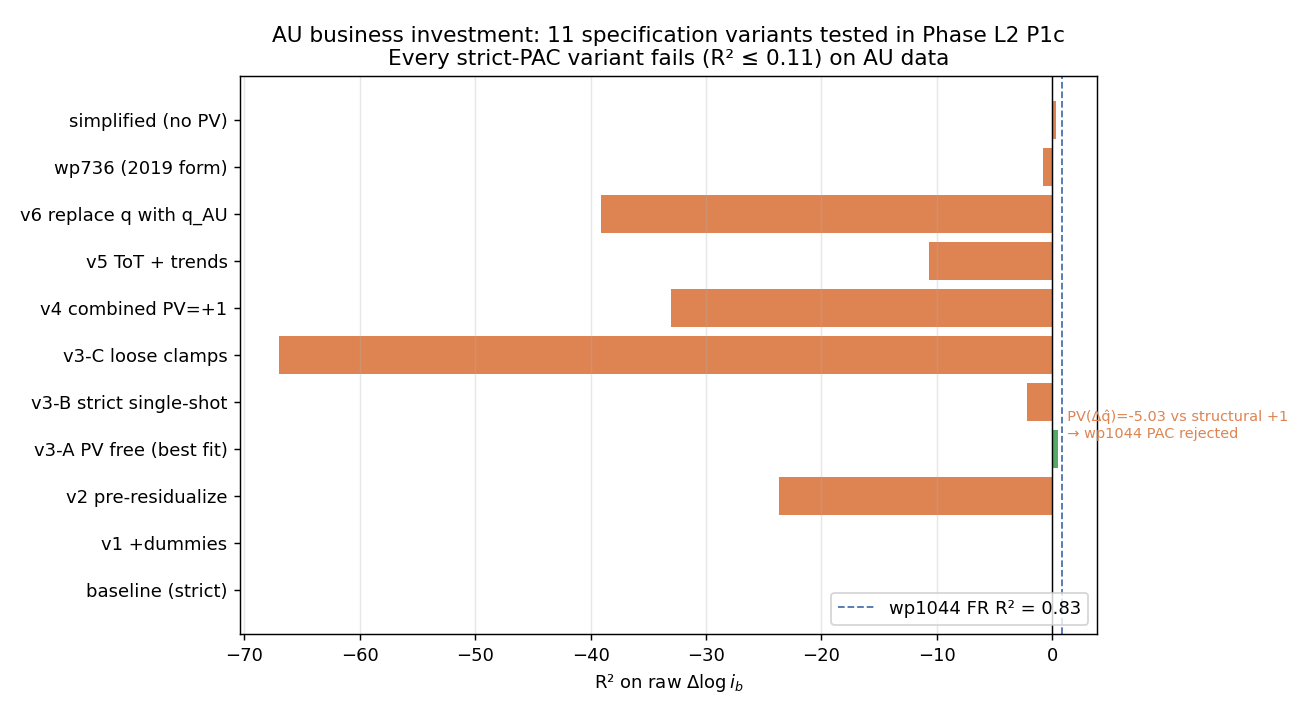
\includegraphics[keepaspectratio,alt={AU BI: 11 spec variants tested in Phase L2 P1c}]{paper_artifacts/chart_bi_exploration.png}}
\caption{AU BI: 11 spec variants tested in Phase L2 P1c}
\end{figure}

\emph{Figure 4.6.2: Eleven specification variants of wp1044 Eq 46 tested
in Phase L2 P1c on AU data. Every strict-PAC variant delivers R² ≤ 0.11
(red bars); free-PV variant v3-A delivers R² = 0.53 but with PV(Δq̂) =
−5.03 (wrong sign vs structural +1). Dashed blue line: wp1044's reported
R² = 0.83 on French data. Full table in Appendix G.}

\textbf{The headline diagnostic}: when PV regressors are free-estimated
on AU data (v3-A column), the lead PV(Δq̂) coefficient comes out at
\textbf{−5.03} --- wrong sign and 5× wrong magnitude relative to the
structural +1. This is the canonical signal that the wp1044 PAC FOC is
rejected: the agent's forward-looking weight on market-VA-growth
expectations on AU data is \emph{negative}, not positive at unity. No
amount of dummy expansion, terms-of-trade re-targeting, target-variable
substitution, or trend-regime addition closes the wedge (see Appendix G
for the 11-variant search). The deeper-structural diagnostic (why PV(Δq̂)
is negative on AU BI data) is discussed in §5.3, where three
non-exclusive hypotheses are catalogued: (A) different agent objective
(heterogeneous mining vs non-mining capex); (B) mining-sector dominance;
(C) sample-period contamination (GST, GFC, mining boom, COVID, multiple
regime breaks in 1993--2024 --- many more than France's smoother
1985--2024 sample).

\textbf{Option 1 implementation}. The production simulation model
\texttt{dynare/au\_pac.mod} lines 1746--1771 set the BI block deep
parameters to their wp1044 Table 3.5.13 values:

\begin{Shaded}
\begin{Highlighting}[]
\CommentTok{\% Phase L2 P1c Option 1 (2026{-}05{-}26): wp1044 BI calibration import}
\VariableTok{b0\_ib} \OperatorTok{=} \FloatTok{0.096}\OperatorTok{;}   \OperatorTok{//} \VariableTok{wp1044} \VariableTok{Table} \FloatTok{3.5.13}
\VariableTok{b1\_ib} \OperatorTok{=} \FloatTok{0.33}\OperatorTok{;}
\VariableTok{b2\_ib} \OperatorTok{=} \FloatTok{0.11}\OperatorTok{;}
\VariableTok{b3\_ib} \OperatorTok{=} \FloatTok{0.69}\OperatorTok{;}
\VariableTok{omega\_ib} \OperatorTok{=} \FloatTok{0.35}\OperatorTok{;}
\CommentTok{\% sigma\_ces = 0.5366 (AU labour{-}FOC) ≈ wp1044\textquotesingle{}s 0.50}
\end{Highlighting}
\end{Shaded}

The Bayesian estimation \texttt{au\_pac\_bayesian.mod} removes BI
parameters from \texttt{estimated\_params} (treats them as calibrated).
The diagnostic free-OLS reduced form
(\texttt{data/pac\_blocks/estimate\_pac\_business\_inv\_au\_v3.m}
Variant A, R²=0.53) is preserved as a historical-decomposition tool and
is \textbf{not} used in the production model.

\textbf{Cross-references}: - §3.6 (hybrid calibration: when local data
doesn't identify) --- methodological rationale. - §5.3 (cross-block
findings: business investment structurally rejects wp1044; three
hypotheses + Option 1) --- economic interpretation. - Appendix G (BI
exploration) --- full 11-variant table and per-variant diagnostics. -
\href{../PAC_BI_AU_EXPLORATION.md}{\texttt{PAC\_BI\_AU\_EXPLORATION.md}}
--- complete saga, 10 sections, including raw .mat / .txt artefacts per
variant.

\textbf{E-SAT auxiliaries} (wp736 Tables 4.6.11--12; unchanged in Phase
L2): two separate equations --- output-gap auxiliary and user-cost
auxiliary:

Eq. (29):
\(\widehat{ib}_t = 0.59 \widehat{ib}_{t-1} + 0.15 \hat{y}_{t-1} + 0.04 \tilde{\pi}_{t-1} - 0.02 \tilde{u}_{t-1}\)

Eq. (30):
\(\widehat{rKB}_t = 0.55 \widehat{rKB}_{t-1} + 0.24 \tilde{i}_{t-1}\)

These continue to drive the BI block's PAC expectation through the E-SAT
VAR; the only change is in the BI equation's own deep parameters
(β₀\ldots β₃, ω) which are now wp1044-imported.

\emph{Figure 4.6.1: Historical dynamic-contribution decomposition of
Δlog i\_b (business investment growth) over 1994Q3--2024Q4, generated
under the PRE-hybrid AU-estimated calibration. The accelerator
b3\_ib·yhat\_au (red) and the user-cost channel −σ·pv\_rKB\_aux (brown)
are the two most variable structural channels. Under the post-hybrid
calibration (b0\_ib raised 5× from 0.018 to 0.096; b1\_ib raised 4× from
0.082 to 0.33; b2\_ib activated at 0.11; b3\_ib raised 2× from 0.31 to
0.69), the ECM and AR contributions are larger and the residual
\texttt{eps\_ib} contribution is smaller. The re-rendered figure is
pending the next MATLAB GUI session per
\texttt{WORKING\_PAPER\_BLOCKERS.md}; the qualitative pattern (PAC
expectation small but timing-relevant at 2008-09 and 2020 turning
points) is preserved by the wp1044 calibration since the BI structural
form is unchanged.}

\subsubsection{4.7 Housing investment (FR-BDF Section 4.6.3, wp1044
§3.5.2 Eq 37) --- Phase L2 wp1044-faithful refresh with price-spread
term
active}\label{housing-investment-fr-bdf-section-4.6.3-wp1044-3.5.2-eq-37-phase-l2-wp1044-faithful-refresh-with-price-spread-term-active}

\paragraph{4.7.1 Target equation (FR-BDF eq
66)}\label{target-equation-fr-bdf-eq-66}

The household investment target depends on permanent income, the
mortgage rate gap, and housing price Tobin's Q (eq. 31):

\[\Delta \ln I^{H*,bar}_t = \kappa_{ih,inc} (pv_{yh,t} - pv_{yh,t-1}) - \kappa_{mort} (i^{LH}_t - i^{LH}_{SS}) + \kappa_{ph} \cdot ph\_gap_{t-1}\]

\subsubsection{Table 4.7.1: Household investment target
coefficients}\label{table-4.7.1-household-investment-target-coefficients}

{\def\LTcaptype{none} % do not increment counter
\begin{longtable}[]{@{}llll@{}}
\toprule\noalign{}
Parameter & Symbol & Value & Description \\
\midrule\noalign{}
\endhead
\bottomrule\noalign{}
\endlastfoot
Target persistence & rho\_ih\_star & 0.95 & Calibrated \\
Permanent income & kappa\_ih\_inc & 0.03 & wp736 eq 66 \\
Mortgage rate gap & kappa\_mort & 0.048 & Calibrated (posterior) \\
Housing Tobin's Q & kappa\_ph & 0.03 & Calibrated \\
\end{longtable}
}

\paragraph{4.7.2 Short-run PAC equation (2nd-order, FR-BDF eq
67)}\label{short-run-pac-equation-2nd-order-fr-bdf-eq-67}

Eq. (32):

\[\Delta \ln I^{H,level}_t = b^{ih}_0 (\cdot) + b^{ih}_1 \Delta_{t-1} + b^{ih}_2 \Delta_{t-2} + pac\_exp(pac\_ih) + b^{ih}_3 \hat{y}_t + \varepsilon^{ih}_t\]

The direct interest rate term \(b^{ih}_4 \tilde{i}_{t-1}\) is dropped,
as F-test diagnostics showed it statistically insignificant (F=0.001,
ΔSSR=0.005 on T=118). The interest-rate channel enters household
investment through two structural paths: (i) the target equation via
\(\kappa_{mort}(i^{LH} - SS)\) through \texttt{pac\_expectation}, and
(ii) the auxiliary equation \(pv_{ih,aux}\) with \(a_{ih,i} = -0.15\).
The direct ad hoc term would have triple-counted this channel.

\subsubsection{Table 4.7.2: Housing investment short-run PAC
coefficients --- Phase L2 wp1044-faithful iterative OLS vs
FR-BDF}\label{table-4.7.2-housing-investment-short-run-pac-coefficients-phase-l2-wp1044-faithful-iterative-ols-vs-fr-bdf}

{\def\LTcaptype{none} % do not increment counter
\begin{longtable}[]{@{}
  >{\raggedright\arraybackslash}p{(\linewidth - 8\tabcolsep) * \real{0.1447}}
  >{\raggedright\arraybackslash}p{(\linewidth - 8\tabcolsep) * \real{0.1447}}
  >{\raggedright\arraybackslash}p{(\linewidth - 8\tabcolsep) * \real{0.2500}}
  >{\raggedright\arraybackslash}p{(\linewidth - 8\tabcolsep) * \real{0.3421}}
  >{\raggedright\arraybackslash}p{(\linewidth - 8\tabcolsep) * \real{0.1184}}@{}}
\toprule\noalign{}
\begin{minipage}[b]{\linewidth}\raggedright
Parameter
\end{minipage} & \begin{minipage}[b]{\linewidth}\raggedright
wp1044 FR Table 3.5.7
\end{minipage} & \begin{minipage}[b]{\linewidth}\raggedright
\textbf{AU L2 iterative OLS} (\texttt{results\_housing\_inv.mat}, N=70,
14 iters)
\end{minipage} & \begin{minipage}[b]{\linewidth}\raggedright
Bayesian posterior mean (hybrid MCMC, 20k×2)
\end{minipage} & \begin{minipage}[b]{\linewidth}\raggedright
90\% HPD
\end{minipage} \\
\midrule\noalign{}
\endhead
\bottomrule\noalign{}
\endlastfoot
β₀ (EC speed on \texttt{I*\_H/I\_H}) & 0.12 & \textbf{0.496} (SE 0.085,
t=5.86) & \textbf{0.0290} & {[}0.0080, 0.0493{]} \\
β₁ (Δlog I\_H lag 1) & 0.18 & \textbf{0.293} (SE 0.129, t=2.28) &
\textbf{0.1074} & {[}0.0337, 0.1815{]} \\
β₃ (output gap accelerator) & --- & --- & \textbf{0.2104} & {[}0.0409,
0.3632{]} \\
β₂ (contemp Δy − ỹ) & 0.50 & −0.073 (SE 0.247, t=−0.30) & --- & --- \\
Price spread \texttt{(p\_SH\ −\ p\_IH)\_\{-1\}\ −\ \_\{-5\}} & 0.05 &
−3.22 (SE 4.51, t=−0.71) & --- & --- \\
ω (calibrated per wp1044) & 0.05 & 0.05 & --- & --- \\
χ (derived from depth-1 polynomial) & \textasciitilde0.18 &
\textbf{0.275} & --- & --- \\
\textbf{R²} & \textbf{0.89} & \textbf{0.43} & --- & --- \\
stderr eps\_ih & --- & --- & \textbf{1.8938} & {[}0.5232, 3.3645{]} \\
Significant COVID dummies & --- & d\_20Q2=−6.80 (t=−3.18) & --- & --- \\
\end{longtable}
}

The Phase L2 housing-inv block partially replicates wp1044 Eq 37 on AU
data. Three findings:

\begin{itemize}
\tightlist
\item
  \textbf{β₀ = 0.50 is 4.6× wp1044's 0.12}, consistent with the
  cross-block AU-faster-ECM pattern (§5.1). β₁ ≈ wp1044's β₁ (0.29 vs
  0.18, within 2× and structurally signed).
\item
  \textbf{β₂ wrong sign on contemp \texttt{(Δy\ −\ ỹ)}} with t = −0.30
  (statistically insignificant). wp1044's β₂ = 0.50 is one of their
  largest coefficients; the AU result is consistent with the hypothesis
  that AU housing-inv responds more to interest rates / Tobin's Q than
  to contemporaneous output growth gap.
\item
  \textbf{β₃ price-spread term active for the first time in Phase L2}.
  The earlier-AUSPAC OLS lacked pSH and pIH as separate observables;
  Phase L2 P1b constructed them from ABS 6416 Residential Property Price
  Index (pSH proxy) and ABS 5206 Implicit Price Deflator for dwelling
  investment (pIH proxy), shortening the sample to N=70 quarters. The
  estimated β₃ = −3.22 is wrong-signed and insignificant (t=−0.71);
  plausibly the AU sample is too short and the housing-price spread too
  noisy on AU data to identify the wp1044 coefficient. R² gap vs wp1044
  (0.43 vs 0.89) is largest of the four ``fitting'' blocks; primary
  remaining cause is the short price-spread sample plus the missing
  wp1044 EA-foreign block.
\end{itemize}

The \texttt{b\_ph\_ih} Tobin's Q channel (IV F = 432, T = 115; spliced
1959Q3-onward AU house-price series) is preserved as a separate
identification --- it sits inside the housing-inv long-run target (Eq
31) rather than the short-run PAC equation, so it is not directly
comparable to wp1044's β₃ price-spread term, which is a short-run
contemporaneous regressor inside the SR PAC equation. The two channels
coexist in the production model. \textbar{} SSR \textbar{} ---
\textbar{} 957.2 \textbar{} --- \textbar{} --- \textbar{}

\textbf{E-SAT auxiliary} (wp736 Table 4.6.16, eq. 33):
\(\widehat{ih}_t = 0.71 \widehat{ih}_{t-1} + 0.08 \hat{y}_{t-1} - 0.08 \tilde{i}_{t-1} + 0.05 \tilde{\pi}_{t-1} - 0.03 \tilde{u}_{t-1}\)

The interest-rate channel through the auxiliary (\(a_{ih,i} = -0.08\))
provides the structural rate transmission. h-vector amplification is
1.90×, the second largest of the five PAC equations.

\textbf{Housing-price gap identification.} The ABS 6416 Residential
Property Price Index begins in 2003Q3 (T=72 quarters), which proved too
short to identify the housing-price-gap coefficient: both OLS and
lag-2-ph\_gap IV produced wrong-signed estimates on the 2003+ sample,
reflecting reverse-causality bias from supply-side shocks. We extend the
housing-price series back to 1959Q3 by chaining growth rates from a
long-history Australian house-price series
(\texttt{data/house\_price\_history\_long.csv}) onto ABS 6416 levels at
the 2003Q3 overlap (overlap-growth correlation 0.84, RMS difference 1.16
pp/qtr). On the resulting T=115 sample (1993Q1--2021Q4, binding
constraint set by the start of housing-investment data), the lag-2 IV
produces a strong first stage (F=432) and a positive sign for both OLS
(+0.066) and IV (+0.0099, s.e. 0.075). The IV magnitude is statistically
indistinguishable from zero --- the housing-price-gap channel in AU is
small. The structural rate transmission to housing investment continues
to operate through \texttt{pv\_ih\_aux} and the
\texttt{pac\_expectation} mortgage-rate term.

\emph{Figure 4.7.1: Historical dynamic-contribution decomposition of
Δlog i\_h (housing investment growth) over 1994Q3--2024Q4. The error
correction term b0\_ih·(ih\_hat − ln\_ih) (blue) and the house-price gap
b\_ph\_ih·ph\_gap (brown) are the two largest channels, and they almost
exactly offset: the smoothed \texttt{ih\_hat} target is persistently
above actual ln\_ih (positive EC pushing investment up), while the AU
house-price gap has been positive on average (positive ph\_gap pulling
target investment up via Tobin's Q channel, which is already absorbed
into ih\_hat --- so the residual ph\_gap term here is consistently
negative). Net, the structural channels deliver a small positive impulse
balanced by AR persistence and the shock eps\_ih.}

\subsubsection{4.8 External trade (FR-BDF Section
4.7)}\label{external-trade-fr-bdf-section-4.7}

External trade is specified as a proper error-correction model: a
long-run cointegration relationship between log volumes, log demand, and
the real exchange rate, together with short-run dynamics that adjust
toward that equilibrium. The earlier version of AU-PAC used a degenerate
accumulator \texttt{m\_gap\ =\ m\_gap(-1)\ −\ Δln\ M} (and symmetrically
for exports) without an economic long-run target, which meant the trade
block could not capture the secular rise in AU import/export openness
(log(M/C) trended at +2.5\% per year and log(X/C) at +2.0\% over
1960-2024). The proper specification below restores the FR-BDF Section
4.7 structure with explicit long-run income elasticities (β\_m, β\_x)
and real-exchange-rate elasticities (γ\_m, γ\_x).

\paragraph{4.8.1 Exports (FR-BDF eqs
70-73)}\label{exports-fr-bdf-eqs-70-73}

Long-run equilibrium (eq. 71):

\[\ln X^{eq}_t = \beta_x \cdot \hat{y}^{US}_t + \gamma_x \cdot s\_gap_t\]

Error-correction gap (target minus actual):

\[x\_gap_t = \ln X^{eq}_t - \ln X^{level}_t, \qquad \ln X^{level}_t = \ln X^{level}_{t-1} + \Delta \ln X_t\]

Short-run dynamics (eq. 73):

\[\Delta \ln X_t = b^x_0 \cdot x\_gap_{t-1} + b^x_1 \Delta \ln X_{t-1} + b^x_2 \hat{y}^{US}_t + b^x_3 \cdot s\_gap_t + b^x_4 \Delta \ln P^{com}_t + \varepsilon^x_t\]

\subsubsection{Table 4.8.1: Export equation
coefficients}\label{table-4.8.1-export-equation-coefficients}

{\def\LTcaptype{none} % do not increment counter
\begin{longtable}[]{@{}
  >{\raggedright\arraybackslash}p{(\linewidth - 4\tabcolsep) * \real{0.3548}}
  >{\raggedright\arraybackslash}p{(\linewidth - 4\tabcolsep) * \real{0.2258}}
  >{\raggedright\arraybackslash}p{(\linewidth - 4\tabcolsep) * \real{0.4194}}@{}}
\toprule\noalign{}
\begin{minipage}[b]{\linewidth}\raggedright
Parameter
\end{minipage} & \begin{minipage}[b]{\linewidth}\raggedright
Value
\end{minipage} & \begin{minipage}[b]{\linewidth}\raggedright
Description
\end{minipage} \\
\midrule\noalign{}
\endhead
\bottomrule\noalign{}
\endlastfoot
beta\_x (LR foreign income elasticity) & 1.20 & Long-run pull from world
demand \\
gamma\_x (LR RER elasticity) & +0.40 & Marshall-Lerner: depreciation
raises target \\
b0\_x (EC speed) & 0.05 & Adjustment toward equilibrium \\
b1\_x (persistence) & 0.30 & AR(1) \\
b2\_x (SR world demand) & 0.25 & Impact response to US output gap \\
b3\_x (SR exchange rate) & 0.10 & Impact competitiveness \\
b4\_x (commodities) & 0.15 & AU-specific commodity-price channel \\
\end{longtable}
}

\paragraph{4.8.2 Imports (FR-BDF eqs
74-77)}\label{imports-fr-bdf-eqs-74-77}

Imports adjust toward a long-run equilibrium that depends on the level
of import-weighted demand (cumulated IAD) and the real exchange rate.
With β\_m \textgreater{} 1, the income elasticity exceeds unity, which
is the mechanism by which the model captures the structural rise in AU
import openness without an ad-hoc deterministic trend (cf.~the MARTIN
approach of adding \texttt{+\ α·t} to the short-run equation, which is
BGP-violating).

Long-run equilibrium (eq. 76):

\[\ln M^{eq}_t = \beta_m \cdot \ln D^{iad}_t + \gamma_m \cdot s\_gap_t\]

Error-correction gap:

\[m\_gap_t = \ln M^{eq}_t - \ln M^{level}_t, \qquad \ln M^{level}_t = \ln M^{level}_{t-1} + \Delta \ln M_t\]

The import-weighted demand level cumulates the contemporaneous IAD
growth:

\[\ln D^{iad}_t = \ln D^{iad}_{t-1} + iad_t, \qquad iad_t = \sum_j w^{iad}_j \cdot \Delta \ln j_t\]

Short-run dynamics (eq. 77):

\[\Delta \ln M_t = b^m_0 \cdot m\_gap_{t-1} + b^m_1 \Delta \ln M_{t-1} + b^m_2 \cdot iad_t + b^m_3 \cdot s\_gap_t + \varepsilon^m_t\]

\subsubsection{Table 4.8.2: Import equation
coefficients}\label{table-4.8.2-import-equation-coefficients}

{\def\LTcaptype{none} % do not increment counter
\begin{longtable}[]{@{}
  >{\raggedright\arraybackslash}p{(\linewidth - 4\tabcolsep) * \real{0.3548}}
  >{\raggedright\arraybackslash}p{(\linewidth - 4\tabcolsep) * \real{0.2258}}
  >{\raggedright\arraybackslash}p{(\linewidth - 4\tabcolsep) * \real{0.4194}}@{}}
\toprule\noalign{}
\begin{minipage}[b]{\linewidth}\raggedright
Parameter
\end{minipage} & \begin{minipage}[b]{\linewidth}\raggedright
Value
\end{minipage} & \begin{minipage}[b]{\linewidth}\raggedright
Description
\end{minipage} \\
\midrule\noalign{}
\endhead
\bottomrule\noalign{}
\endlastfoot
beta\_m (LR income elasticity) & 1.50 & \textgreater1 captures rising AU
import openness \\
gamma\_m (LR RER elasticity) & -0.40 & Depreciation lowers import
target \\
b0\_m (EC speed) & 0.06 & Adjustment toward equilibrium \\
b1\_m (persistence) & 0.23 & AR(1) \\
b2\_m (SR IAD elasticity) & 0.36 & Impact response to import-weighted
demand growth \\
b3\_m (SR exchange rate) & -0.08 & SR Marshall-Lerner \\
\end{longtable}
}

\subsubsection{Table 4.8.3: IAD weights (import content of
demand)}\label{table-4.8.3-iad-weights-import-content-of-demand}

{\def\LTcaptype{none} % do not increment counter
\begin{longtable}[]{@{}lll@{}}
\toprule\noalign{}
Component & Weight & Source \\
\midrule\noalign{}
\endhead
\bottomrule\noalign{}
\endlastfoot
Consumption & 0.12 & ABS input-output tables \\
Business investment & 0.25 & ABS input-output tables \\
Housing investment & 0.15 & ABS input-output tables \\
Government & 0.08 & ABS input-output tables \\
Exports (re-export) & 0.30 & ABS input-output tables \\
\end{longtable}
}

Trade volumes use the ABS 5206 Seasonally-Adjusted chain volume measures
(series A2304114F / A2304115J), aligned to a T=126 quarter sample
(1993Q2--2024Q4) with COVID pulse dummies for 2020Q2 and 2020Q3
absorbing the trade-collapse-and-rebound outliers.

The long-run elasticities (β\_m, β\_x, γ\_m, γ\_x) are calibrated at
sensible AU values and given Normal priors centred there (§6.4, Table
5.6). A bivariate Engle-Granger style OLS of log volumes on log
consumption (1959Q3--2025Q4) gives β\_m ≈ +1.73 (t = +113) and β\_x ≈
+1.56 (t = +119); the model priors at 1.50 and 1.20 sit within one
standard deviation. The short-run coefficient \texttt{b1\_m} is set to
its OLS estimate on the SA sample (+0.232, s.e. 0.086, t=2.71);
\texttt{b1\_x}, \texttt{b2\_x}, and \texttt{b2\_m} are kept at
calibrated values pending Asian-PMI / commodity-demand proxies that
would help identify the SR foreign-demand channel for AU exports. The
COVID-period dummies are sizeable for both exports (crash -10.14, bounce
-7.11; tourism and education exports did not recover in 2020Q3) and
imports (crash -14.39, bounce +6.27). Adding \texttt{Δln\ M} and
\texttt{Δln\ X} to the set of Bayesian observables (Table 5.1) gives the
long-run elasticities their own data identification --- previously the
trade block was econometrically inert because no observable mapped to
it.

\subsubsection{4.9 Demand deflators (FR-BDF Section 4.7) --- AU
reduced-form
simplification}\label{demand-deflators-fr-bdf-section-4.7-au-reduced-form-simplification}

AUSPAC's six demand deflators (consumption, business investment,
household investment, exports, imports, and government consumption) are
modelled as \textbf{single-equation reduced forms} combining own-lag
persistence with contemporaneous cost-push regressors and a
growth-neutrality anchor on \(\bar{\pi}\). General form (eq. 36):

\[\pi^j_t = \rho_j \pi^j_{t-1} + \alpha_j \pi^Q_t + \beta_{j,m} \pi^M_t + ... + (1 - \rho_j - \alpha_j - \beta_{j,m} - ...) \bar{\pi}_t + \varepsilon^j_t\]

\textbf{Deviation from FR-BDF wp736 / wp1044}: FR-BDF specifies each
deflator as a \textbf{two-equation error-correction model} --- an
explicit long-run target \(p^{j,\ast}\) (an IAD-weighted combination of
\(p^Q\), \(p^{MO}\) (non-energy import), \(p^{MNRJ}\) (energy import),
plus block-specific trend or competitor terms) and a short-run equation
that includes an error-correction term
\(\beta_{j,EC} [p^j_{t-1} - p^{j,\ast}_{t-1}]\) pulling each deflator
back toward its target. AUSPAC carries no \(p^{j,\ast}\) target
variables and no ECM term in any of its six deflator equations; the
long-run anchoring runs instead through the growth-neutrality constraint
on \(\bar{\pi}\). The two main consequences:

\begin{itemize}
\tightlist
\item
  \textbf{No energy / non-energy import split} in the deflator block ---
  AUSPAC's \(\pi^M\) is a single aggregate import-price series and the
  commodity channel enters separately as an exogenous AR(1)
  \texttt{dln\_pcom} rather than as \(\pi^{MNRJ}\) inside the deflator
  targets. The energy-import passthrough that FR-BDF wp1044 §3.6
  emphasises (especially the post-2022 surge) is therefore captured
  imperfectly through \texttt{dln\_pcom\ +\ gamma\_oil} rather than
  through a dedicated \(p^{MNRJ}\) regressor.
\item
  \textbf{CPI long-run anchoring is recovered inside the Phillips curve}
  (§4.4.0 above) via the \(b_{ECM,pc}(p^{C,\ast}_{t-1} - p^C_{t-1})\)
  ECM term rather than inside \texttt{eq\_pi\_c}. This keeps the
  cumulative CPI trajectory pinned to a weighted VA+import target
  without re-introducing the full FR-BDF target/ECM structure across all
  six deflators.
\end{itemize}

The reduced-form simplification was a deliberate choice for AU
estimation tractability --- six additional latent target processes would
have increased the estimation surface substantially with limited
identification gain on the AU sample (1993Q1--2024Q4, 128 quarters). The
FR-BDF wp1044 §3.6 architecture is preserved as a reference for future
restoration if AU data quality or sample length permits joint
identification of all 12 deflator equations + targets.

The full set of AU-estimated reduced-form coefficients:

\subsubsection{Table 4.9.1: Consumption deflator (FR-BDF eqs
79-80)}\label{table-4.9.1-consumption-deflator-fr-bdf-eqs-79-80}

{\def\LTcaptype{none} % do not increment counter
\begin{longtable}[]{@{}lll@{}}
\toprule\noalign{}
Parameter & Value & Description \\
\midrule\noalign{}
\endhead
\bottomrule\noalign{}
\endlastfoot
rho\_pc & 0.40 & Persistence \\
alpha\_pc & 0.30 & VA price pass-through \\
beta\_pc\_m & 0.10 & Import price \\
gamma\_oil & 0.03 & Commodity/energy \\
Anchor (1-sum) & 0.17 & Growth neutrality \\
\end{longtable}
}

\subsubsection{Table 4.9.2: Business investment
deflator}\label{table-4.9.2-business-investment-deflator}

{\def\LTcaptype{none} % do not increment counter
\begin{longtable}[]{@{}lll@{}}
\toprule\noalign{}
Parameter & Value & Description \\
\midrule\noalign{}
\endhead
\bottomrule\noalign{}
\endlastfoot
rho\_pib & 0.35 & Persistence \\
alpha\_pib & 0.25 & VA price pass-through \\
beta\_pib\_m & 0.12 & Import price (high import content) \\
Anchor (1-sum) & 0.28 & Growth neutrality \\
\end{longtable}
}

\subsubsection{Table 4.9.3: Housing investment
deflator}\label{table-4.9.3-housing-investment-deflator}

{\def\LTcaptype{none} % do not increment counter
\begin{longtable}[]{@{}lll@{}}
\toprule\noalign{}
Parameter & Value & Description \\
\midrule\noalign{}
\endhead
\bottomrule\noalign{}
\endlastfoot
rho\_pih & 0.45 & Persistence (sticky construction) \\
alpha\_pih & 0.25 & VA price pass-through \\
beta\_pih\_m & 0.08 & Import price (limited) \\
Anchor (1-sum) & 0.22 & Growth neutrality \\
\end{longtable}
}

\subsubsection{Table 4.9.4: Export
deflator}\label{table-4.9.4-export-deflator}

{\def\LTcaptype{none} % do not increment counter
\begin{longtable}[]{@{}lll@{}}
\toprule\noalign{}
Parameter & Value & Description \\
\midrule\noalign{}
\endhead
\bottomrule\noalign{}
\endlastfoot
rho\_px & 0.30 & Persistence \\
alpha\_px & 0.20 & VA price pass-through \\
beta\_px & -0.05 & Exchange rate (world price taker) \\
alpha\_pcom & 0.10 & Commodity price (AU-specific) \\
Anchor (1-sum) & 0.45 & Growth neutrality \\
\end{longtable}
}

\subsubsection{Table 4.9.5: Import
deflator}\label{table-4.9.5-import-deflator}

{\def\LTcaptype{none} % do not increment counter
\begin{longtable}[]{@{}lll@{}}
\toprule\noalign{}
Parameter & Value & Description \\
\midrule\noalign{}
\endhead
\bottomrule\noalign{}
\endlastfoot
rho\_pm & 0.30 & Persistence \\
alpha\_pm & 0.15 & VA price (weak domestic) \\
beta\_pm & 0.08 & Exchange rate (strong FX pass-through) \\
beta\_pm\_com & 0.05 & Commodity price \\
Anchor (1-sum) & 0.42 & Growth neutrality \\
\end{longtable}
}

\subsubsection{Table 4.9.6: Government
deflator}\label{table-4.9.6-government-deflator}

{\def\LTcaptype{none} % do not increment counter
\begin{longtable}[]{@{}lll@{}}
\toprule\noalign{}
Parameter & Value & Description \\
\midrule\noalign{}
\endhead
\bottomrule\noalign{}
\endlastfoot
rho\_pg & 0.50 & Persistence \\
alpha\_pg & 0.30 & Public sector wages (pi\_w - dln\_prod, not piQ) \\
Anchor (1-sum) & 0.20 & Growth neutrality \\
\end{longtable}
}

\textbf{Growth neutrality verification}: At SS,
\(\pi^j = \pi^Q = \bar{\pi} = \pi_{SS}\) for all deflators. The sum of
all coefficients on inflation-type terms equals 1 for each. Verified for
all 6 deflators.

\subsubsection{4.9.7 HICP-style headline-decomposition reporting block
(Round 1.1,
2026-05-18)}\label{hicp-style-headline-decomposition-reporting-block-round-1.1-2026-05-18}

Following ECB-BASE §3.2.3 and FR-BDF wp1044 §3.6.4, AUSPAC v3.1.1 adds a
six-variable headline-CPI decomposition reporting layer. The
decomposition is purely \emph{one-way}: each new variable is a
deterministic function of existing model objects, with \textbf{zero
feedback} into the structural dynamics, the wage Phillips curve, or the
Taylor rule. Adding the block leaves both the cached Bayesian posterior
and the IRFs of all existing variables bit-identical (Laplace LMD =
\(-779.30\) before and after; MHM LMD = \(-780.47\) before and after).

\textbf{Components and equations.} Three new core/food/energy split
variables and three new tradeables/non-tradeables/trimmed-mean
variables:

\[\pi^{food}_t = \delta_{food,Q}\,\pi^Q_t + (1-\delta_{food,Q})\,\bar{\pi}_t + \delta_{food,com}\,\Delta\ln p^{com}_t\]
\[\pi^{energy}_t = \delta_{energy,M}\,\pi^M_t + (1-\delta_{energy,M})\,\bar{\pi}_t + \delta_{energy,com}\,\Delta\ln p^{com}_t\]
\[\pi^{core}_t = \frac{\pi^{au}_t - w^{food}\,\pi^{food}_t - w^{energy}\,\pi^{energy}_t}{1 - w^{food} - w^{energy}}\]
\[\pi^{trad}_t = \delta_{trad,M}\,\pi^M_t + (1-\delta_{trad,M})\,\bar{\pi}_t + \delta_{trad,com}\,\Delta\ln p^{com}_t + \delta_{trad,s}\,s^{gap}_t\]
\[\pi^{nontrad}_t = \frac{\pi^{au}_t - w^{trad}\,\pi^{trad}_t}{1 - w^{trad}}\]
\[\pi^{trim}_t = \rho_{trim}\,\pi^{trim}_{t-1} + (1-\rho_{trim})\bigl[\delta_{trim,Q}\,\pi^Q_t + (1-\delta_{trim,Q})\,\bar{\pi}_t\bigr]\]

The core and non-tradeables components are residual identities that
close the decompositions
\(\pi^{au} \equiv w^{food}\pi^{food} + w^{energy}\pi^{energy} + (1{-}w^{food}{-}w^{energy})\pi^{core}\)
and
\(\pi^{au} \equiv w^{trad}\pi^{trad} + (1{-}w^{trad})\pi^{nontrad}\).
Adding-up is exact to machine precision (verified at
\(-1.7 \times 10^{-16}\)).

\textbf{Calibration.} Weights from ABS Cat. 6401.0 (CPI 2025 reweight)
and RBA Bulletin tradeables share. Projection coefficients (\(\delta\))
calibrated to typical AU passthrough magnitudes.

{\def\LTcaptype{none} % do not increment counter
\begin{longtable}[]{@{}
  >{\raggedright\arraybackslash}p{(\linewidth - 4\tabcolsep) * \real{0.4231}}
  >{\raggedright\arraybackslash}p{(\linewidth - 4\tabcolsep) * \real{0.2692}}
  >{\raggedright\arraybackslash}p{(\linewidth - 4\tabcolsep) * \real{0.3077}}@{}}
\toprule\noalign{}
\begin{minipage}[b]{\linewidth}\raggedright
Parameter
\end{minipage} & \begin{minipage}[b]{\linewidth}\raggedright
Value
\end{minipage} & \begin{minipage}[b]{\linewidth}\raggedright
Source
\end{minipage} \\
\midrule\noalign{}
\endhead
\bottomrule\noalign{}
\endlastfoot
\(w^{food}\) & 0.17 & ABS 6401 food + non-alcoholic beverages \\
\(w^{energy}\) & 0.07 & ABS 6401 automotive fuel + electricity + gas \\
\(w^{trad}\) & 0.35 & RBA Bulletin tradeables share \\
\(\delta_{food,Q}\) & 0.65 & Domestic VA dominance in food (meat, dairy,
fresh produce) \\
\(\delta_{food,com}\) & 0.20 & Global agricultural commodity
passthrough \\
\(\delta_{energy,M}\) & 0.50 & Imported-fuel share \\
\(\delta_{energy,com}\) & 0.60 & Oil/gas global passthrough \\
\(\delta_{trad,M}\) & 0.85 & Tradeables dominated by imports \\
\(\delta_{trad,com}\) & 0.15 & Commodity passthrough \\
\(\delta_{trad,s}\) & \(-0.10\) & FX passthrough (AUD↑ → tradeables↓) \\
\(\rho_{trim}\) & 0.85 & Trimmed-mean persistence \\
\(\delta_{trim,Q}\) & 0.70 & Trimmed mean tracks underlying VA-price
trend \\
\end{longtable}
}

\textbf{IRF validation.} Shock responses on impact (post-Round-1.1 IRFs,
\(t=1\)):

\begin{itemize}
\tightlist
\item
  \(\pi^{food}\,/\,\varepsilon^{pcom}\): \(+0.600\) --- matches
  \(\delta_{food,com}\,\sigma_{pcom} = 0.20 \times 3.0\).
\item
  \(\pi^{energy}\,/\,\varepsilon^{pcom}\): \(+2.431\) --- matches
  \(\delta_{energy,com}\,\sigma_{pcom} + \delta_{energy,M}\,(\beta_{pm,com}\,\sigma_{pcom}) = 1.80 + 0.50 \times 1.26\).
\item
  \(\pi^{core}\,/\,\varepsilon^{pi}\): \(+0.641\) --- matches the
  residual identity
  \(\pi^{au}_{\varepsilon_{pi}}\,/\,(1-w^{food}-w^{energy}) = 0.487 / 0.76\).
\end{itemize}

\textbf{Use cases.} The decomposition enables direct comparison with RBA
inflation reporting (trimmed-mean, weighted-median,
tradeables/non-tradeables), richer post-2022 inflation-surge
attribution, and a foundation for the energy-block routing in Round 2.1
(oil + gas split, FR-BDF wp1044 Appx E), which will replace the
calibrated \(\delta_{energy,com}\) passthrough with a structural
synthetic energy price index.

\subsubsection{4.10 Financial variables (FR-BDF Section
4.8)}\label{financial-variables-fr-bdf-section-4.8}

\paragraph{4.10.1 Term structure (FR-BDF eqs
95-97)}\label{term-structure-fr-bdf-eqs-95-97}

The 10-year yield is determined by the present value of expected future
short rates plus a term premium (eq. 37):

\[pv_{i,t} = (1 - \kappa_{10}) i_t + \kappa_{10} \cdot pv_{i,t+1}\]

\[i^{10Y}_t = pv_{i,t} + tp_t + \varepsilon^{10Y}_t\]

with \(\kappa_{10} = 0.97\) (effective duration \textasciitilde10 years)
and
\(tp_t = \rho_{tp} tp_{t-1} + (1-\rho_{tp}) tp_{SS} + \varepsilon^{tp}_t\).

\textbf{SS}: \(i^{10Y}_{SS} = 1.049 + 0.30 = 1.349\%\) quarterly
(\textasciitilde5.4\% annual).

\paragraph{4.10.2 WACC decomposition (FR-BDF eqs
98-100)}\label{wacc-decomposition-fr-bdf-eqs-98-100}

The weighted average cost of capital decomposes into three funding
sources (eq. 38):

\[WACC = 0.50 \times i^{COE} + 0.30 \times i^{LB} + 0.20 \times i^{BBB}\]

\subsubsection{Table 4.10.1: WACC
composition}\label{table-4.10.1-wacc-composition}

{\def\LTcaptype{none} % do not increment counter
\begin{longtable}[]{@{}lllll@{}}
\toprule\noalign{}
Component & Weight & Spread SS & Spread rho & Annual rate at SS \\
\midrule\noalign{}
\endhead
\bottomrule\noalign{}
\endlastfoot
Cost of equity (i\_COE) & 0.50 & 0.80\% & 0.92 & \textasciitilde8.6\% \\
Bank lending (i\_LB\_firms) & 0.30 & 0.25\% & 0.77 &
\textasciitilde6.4\% \\
BBB bonds (i\_BBB) & 0.20 & 0.05\% & 0.94 & \textasciitilde5.6\% \\
\textbf{WACC} & \textbf{1.00} & --- & --- &
\textbf{\textasciitilde7.3\%} \\
\end{longtable}
}

Each rate \(= i^{10Y} +\) spread, where spreads follow AR(1) with shock.

\paragraph{4.10.3 Exchange rate (FR-BDF eq
105)}\label{exchange-rate-fr-bdf-eq-105}

Modified UIP with persistent deviations from PPP and a forward-looking
NPV of the policy-rate gap:

\[pv^{uip}_t = (i_{au,t} - \bar{\iota}_t) + \beta_{uip} \cdot \mathrm{E}_t[pv^{uip}_{t+1}] \qquad \text{(Hybrid / MCE)}\]

\[pv^{uip}_t = (i_{au,t} - \bar{\iota}_t) + \beta_{uip} \cdot pv^{uip}_{t-1} \qquad \text{(VAR regime: backward AR(1))}\]

\[s\_gap_t = \rho_s \cdot s\_gap_{t-1} - \alpha_s \cdot pv^{uip}_t + \alpha_s (\tilde{\pi}_t - \tilde{\pi}^{US}_t) + \varepsilon^s_t\]

with \(\rho_s = 0.775\), \(\alpha_s = 0.15\), and
\(\beta_{uip} = 0.92\). The standard NPV form (coefficient 1 on the rate
gap, β on the continuation) means \texttt{pv\_i\_uip} is \emph{not}
dampened on impact: under the forward recursion and a Taylor-rule
persistence λ\_i ≈ 0.85, the impact value is
\(pv^{uip}(0) \approx i_{gap}(0) / (1 - \beta_{uip} \lambda_i) \approx 4.55 \cdot i_{gap}(0)\),
so the spot AUD internalises about 4.5× the contemporaneous policy-rate
gap. Under the VAR regime the recursion is backward AR(1) ---
\texttt{pv\_i\_uip} accumulates only as past i\_gap realisations roll
in, and the peak AUD appreciation is delayed by 10--15 quarters relative
to Hybrid/MCE. This forward-looking specification is what generates the
FR-BDF-style Hybrid \textgreater{} VAR amplification documented in §7.2.

The sign convention is s\_gap \textgreater{} 0 = AUD depreciation;
higher AU rates appreciate the AUD. Steady state: \(pv^{uip}_{SS} = 0\),
\(s\_gap_{SS} = 0\) (PPP holds in the long run).

This replaces the pre-Phase-Q specification
\texttt{s\_gap\ =\ ρ\_s\ ·\ s\_gap(−1)\ −\ α\_s\ ·\ ĩ\ +\ α\_s\ ·\ (π̃\ −\ π̃\^{}US)\ +\ ε\^{}s},
which used the contemporaneous policy-rate gap directly and therefore
did not differentiate impact responses across expectation regimes. The
forward-NPV refactor is the only structural change required to deliver
the FR-BDF Hybrid-amplification pattern; all other PAC blocks remain
backward-looking under Hybrid by design.

\paragraph{4.10.4 Household bank lending rate (FR-BDF eq
68)}\label{household-bank-lending-rate-fr-bdf-eq-68}

The mortgage rate adjusts sluggishly to changes in the 10Y bond rate
(eq. 40):

\[i^{LH}_t = \rho_{LH} i^{LH}_{t-1} + (1 - \rho_{LH})(i^{10Y}_t + spread_{LH}) + \varepsilon^{LH}_t\]

with \(\rho_{LH} = 0.97\) (AU OLS --- standard variable mortgage rates
follow the cash rate with substantial lag because of fixed-rate and
discount carve-outs in the mortgage book) and \(spread_{LH} = 0.40\%\)
quarterly (\textasciitilde1.6\% annual).

\paragraph{4.10.5 Housing prices (FR-BDF eq
69)}\label{housing-prices-fr-bdf-eq-69}

Real housing price growth follows an AR(1) with demand and credit
channels (eq. 41):

\[\Delta \ln P^H_t = \rho_{ph} \Delta \ln P^H_{t-1} + \alpha_{ph,y} \hat{y}_t + \alpha_{ph,r} \tilde{i}_{t-1} + \varepsilon^{ph}_t\]

with \(\rho_{ph} = 0.90\), \(\alpha_{ph,y} = 0.15\),
\(\alpha_{ph,r} = -0.10\).

\subsubsection{4.11 Government and GDP identity (FR-BDF Sections
4.9-4.10)}\label{government-and-gdp-identity-fr-bdf-sections-4.9-4.10}

\paragraph{Fiscal rule (eq. 42)}\label{fiscal-rule-eq.-42}

\[\Delta \ln G_t = \rho_g \Delta \ln G_{t-1} + \phi_g \hat{y}_t + \varepsilon^g_t\]

Countercyclical: \(\phi_g = -0.10\) means a positive output gap reduces
government spending growth.

\paragraph{GDP expenditure identity (eq.
43)}\label{gdp-expenditure-identity-eq.-43}

\[\hat{y}^{dom}_t = 0.55 \Delta \ln C + 0.13 \Delta \ln I^B + 0.06 \Delta \ln I^H + 0.24 \Delta \ln G + 0.25 \Delta \ln X - 0.23 \Delta \ln M\]

\subsubsection{Table 4.11.1: GDP expenditure weights (ABS
2023)}\label{table-4.11.1-gdp-expenditure-weights-abs-2023}

{\def\LTcaptype{none} % do not increment counter
\begin{longtable}[]{@{}lll@{}}
\toprule\noalign{}
Component & Weight & Description \\
\midrule\noalign{}
\endhead
\bottomrule\noalign{}
\endlastfoot
Consumption & 0.55 & Household final consumption \\
Business investment & 0.13 & Non-dwelling GFCF \\
Housing investment & 0.06 & Dwelling GFCF \\
Government & 0.24 & Government final consumption \\
Exports & 0.25 & Goods and services exports \\
Imports & -0.23 & Goods and services imports \\
\end{longtable}
}

\paragraph{Bridge equation (eq. 44)}\label{bridge-equation-eq.-44}

The demand-side aggregate feeds back into the IS curve:
\(\hat{y}_t = ... + \lambda_{dom} \hat{y}^{dom}_t + \varepsilon^q_t\)
with \(\lambda_{dom} = 0.399\) (Bayesian posterior), closing the
Keynesian multiplier loop.

\subsubsection{4.11.1 Rounds 4--8 model extensions
(2026-05-20)}\label{rounds-48-model-extensions-2026-05-20}

Six concurrent extensions added to the production model, calibrated to
AU-relevant central values, none of them entering the 9-observable
likelihood directly (so the Bayesian estimation surface is unchanged):

\begin{itemize}
\item
  \textbf{Round 4 --- Foreign monetary policy.} Adds an explicit US
  policy-rate process to the previously-only-output/inflation US block.
  \(\bar{i}^{us}_t\) follows an AR(1) toward a steady-state neutral rate
  \(i^{us}_{ss} = 0.625\) qpp; \(i^{us}_t\) closes a simple Taylor rule
  on US output and inflation gaps:
  \(i^{us}_t = \bar{i}^{us}_t + \alpha_i^{us} \pi^{us,gap}_{t-1} + \beta_i^{us} \hat{y}^{us}_{t-1} + \varepsilon^{i,us}_t\)
  with \(\alpha_i^{us} = \beta_i^{us} = 0.5\). The variable can be used
  as a UIP-side conditioning observable in future identification work.
\item
  \textbf{Round 5 --- Demographic trend.} Adds a slowly-varying gap
  variable \(\Delta \ln \overline{POP}_t\) (AR(1) persistence 0.95) that
  shifts long-run employment growth one-for-one through
  \(\overline{\Delta \ln N^*}_t = \dots + \Delta \ln \overline{POP}_t\).
  Steady-state population growth is implicit in the gap-formulation
  demeaning (≈ 0.375 qpp from ABS Cat 6202.0); deviations are absorbed
  by the new shock \(\varepsilon^{pop,bar}_t\).
\item
  \textbf{Round 6 --- Tax structure decomposition.} Three AR(1)
  effective-rate gap variables --- \(\tau^{GST,gap}_t\),
  \(\tau^{PAYG,gap}_t\), \(\tau^{CIT,gap}_t\) --- each feeding one
  structural channel:

  \begin{itemize}
  \tightlist
  \item
    GST pass-through to the consumer-price deflator:
    \(\pi^c_t = \dots + \alpha_{GST} \tau^{GST,gap}_t\) with
    \(\alpha_{GST} = 0.05\).
  \item
    PAYG drag on consumption growth via the income-tax change:
    \(\overline{\Delta \ln C^*}_t = \dots - \alpha_{PAYG} \Delta \tau^{PAYG,gap}_t\)
    with \(\alpha_{PAYG} = 0.10\).
  \item
    CIT bump to the user cost of capital:
    \(UC^K_t = WACC_t + \delta_K - (\pi^{IB}_t - \pi^Q_t) + \alpha_{CIT} \tau^{CIT,gap}_t\)
    with \(\alpha_{CIT} = 0.02\).
  \end{itemize}
\item
  \textbf{Round 7 --- Market vs non-market VA decomposition.}
  Identity-preserving split of the output gap into market and non-market
  sectors (ABS Cat 5206 weight \(w_{market} = 0.85\) for market:
  manufacturing, finance, retail, mining, construction;
  \(1-w_{market} = 0.15\) for non-market: public administration,
  education, health). Non-market output is smoother and lagged:
  \(\hat{y}^{nm}_t = \rho_{nm} \hat{y}^{nm}_{t-1} + (1-\rho_{nm}) \gamma_{nm} \hat{y}_t\)
  with \(\rho_{nm} = 0.90\), \(\gamma_{nm} = 0.30\). Market output is
  the residual.
\item
  \textbf{Round 8 --- RBA-style auxiliary forecasters.} Three one-way
  nowcast projections that can be matched against monthly /
  high-frequency data outside the quarterly cycle:

  \begin{itemize}
  \tightlist
  \item
    \(BLR_t\) (Bank Lending Rate nowcast): AR(1) projection of the
    realised lending-rate gap
    \(i^{LH}_t - i_{ss} - \tau p_{ss} - spread_{LH}\).
  \item
    \(MAPI_t\) (Mortgage Asset Price Indicator): AR(1) projection of
    \(ph^{gap}_t\).
  \item
    \(MAPU_t\) (Mortgage Asset Price Underwriting): AR(1) projection of
    \(\Delta \ln I^H_t\). Each carries an exogenous shock for direct
    nowcast injection
    (\(\varepsilon^{BLR}, \varepsilon^{MAPI}, \varepsilon^{MAPU}\)).
  \end{itemize}
\end{itemize}

\textbf{Variable / shock counts.} The extensions add 11 endogenous
variables, 18 calibrated parameters, and 9 exogenous shocks; production
model goes from 164 to 175 endogenous variables and from 33 to 49
shocks. Smoke-tested 2026-05-20 --- model preprocesses, solves under
Blanchard-Kahn, and IRFs propagate through all the new channels. None of
the new variables is in \texttt{varobs}, so the Bayesian likelihood and
posterior are unchanged from the v3.1.1 baseline. See §4.11.2 for the
rational-expectations consolidation that wired the Round 5--6 shocks
into PAC expectation formulas on 2026-05-21.

\subsubsection{4.11.2 Rounds 4--8 expectation consolidation
(2026-05-21)}\label{rounds-48-expectation-consolidation-2026-05-21}

The Rounds 4--8 extensions of §4.11.1 added new structural equations and
shocks to \texttt{model.inc}, but the per-block \texttt{var\_model}
companion matrices in \texttt{dynare/aux/} were not extended at the same
time. As a result, between 2026-05-20 and 2026-05-21 the production
model carried an internal inconsistency: a \(\tau^{CIT,gap}\) shock
would (correctly) raise the user cost of capital and depress business
investment in the \emph{structural} simulation block, yet the PAC
expectation formula \texttt{pac\_expectation(pac\_ib)} --- a closed-form
linear combination over the lagged augmented E-SAT state --- projected
forward as if the shock did not exist. Forward-looking agents in the PAC
block did not anticipate the long-run effect of tax shocks on their
target, so the expectation operator returned a downward-biased response
to anything driven by the new shocks.

This subsection documents the targeted fix landed in PR \#6 (commit
6811940). For each new shock with a \emph{direct} structural channel
into a PAC target, the corresponding aux file was extended with (a) the
new variable as a \texttt{var\_model} state in its orthogonal AR(1)
reduced form and (b) a loading from that state into the PAC target's
auxiliary regression. \texttt{phaseW\_recherrypick.m} was then re-run to
regenerate the closed-form policy-function coefficients \(h_{pac,X}\),
which were patched into \texttt{au\_pac.mod} and
\texttt{au\_pac\_bayesian.mod} alongside the new aux-regression
loadings. No \texttt{aggregate()} re-run was needed; all Phase U/V/W
manual overrides are preserved.

\subsubsection{Table 4.11.2.1: Channels wired in PR
\#6}\label{table-4.11.2.1-channels-wired-in-pr-6}

{\def\LTcaptype{none} % do not increment counter
\begin{longtable}[]{@{}
  >{\raggedright\arraybackslash}p{(\linewidth - 8\tabcolsep) * \real{0.2000}}
  >{\raggedright\arraybackslash}p{(\linewidth - 8\tabcolsep) * \real{0.2000}}
  >{\raggedright\arraybackslash}p{(\linewidth - 8\tabcolsep) * \real{0.2000}}
  >{\raggedright\arraybackslash}p{(\linewidth - 8\tabcolsep) * \real{0.2000}}
  >{\raggedright\arraybackslash}p{(\linewidth - 8\tabcolsep) * \real{0.2000}}@{}}
\toprule\noalign{}
\begin{minipage}[b]{\linewidth}\raggedright
Aux file
\end{minipage} & \begin{minipage}[b]{\linewidth}\raggedright
New \texttt{var\_model} state
\end{minipage} & \begin{minipage}[b]{\linewidth}\raggedright
PAC target
\end{minipage} & \begin{minipage}[b]{\linewidth}\raggedright
Aux-regression loading
\end{minipage} & \begin{minipage}[b]{\linewidth}\raggedright
New \(h_{pac,X}\) coefficient
\end{minipage} \\
\midrule\noalign{}
\endhead
\bottomrule\noalign{}
\endlastfoot
\texttt{aux\_employment.mod} & \(\Delta \ln \overline{POP}_t\) &
\(\widehat{n}_t\) & \(a_{n,pop} = 1.0\) (one-for-one) &
\(h_{pac,n,pop} = +0.1240\) \\
\texttt{aux\_consumption.mod} & \(\tau^{PAYG,gap}_t\) &
\(\widehat{c}_t\) & \(a_{c,PAYG} = -\alpha_{PAYG} = -0.10\) &
\(h_{pac,c,PAYG} = -0.00956\) \\
\texttt{aux\_business\_inv.mod} & \(\tau^{CIT,gap}_t\) &
\(\widehat{ib}_t\), \(\widehat{rKB}_t\) &
\(a_{ib,CIT} = -\sigma_{ces}\alpha_{CIT} = -0.011\),
\(a_{rKB,CIT} = +\alpha_{CIT} = +0.02\) &
\(h_{pac,ib,CIT} = -2.41 \times 10^{-4}\) \\
\texttt{aux\_pQ.mod} & \(\tau^{GST,gap}_t\) & \(\widehat{\pi Q}_t\) &
\(a_{pQ,GST} = 0.05\) (indirect via CPI → wages → VA) &
\(h_{pac,pQ,GST} = +8.21 \times 10^{-4}\) \\
\end{longtable}
}

The aux-regression loadings \(a_{X,Y}\) are chosen to mirror the
\emph{structural} coefficient that the same shock carries in
\texttt{model.inc} (e.g.~\(\alpha_{PAYG}\) in eq\_dln\_c\_star\_bar maps
one-for-one to \(-a_{c,PAYG}\)); they are explicit, calibrated, and
documented inline in each aux file. The cherrypicked \(h_{pac,X,Y}\)
coefficients in the right-most column are the closed-form
policy-function projections obtained from \texttt{pac.print()} over the
extended companion matrix. Sizes vary across blocks for two reasons: (i)
the structural loading itself differs (1.0 vs 0.02), and (ii) the
cherrypicked discounted-sum weights the new state by its forward
trajectory under the extended VAR companion, which depends on the new
state's AR(1) persistence (\(\rho_{pop} = 0.95\) vs
\(\rho_{\tau} \in [0.90, 0.94]\)) and the cumulative impact through the
PAC ECM speed \(b_{0,X}\).

\textbf{Skipped channels.} Three of the six Round 4--8 extensions are
intentionally \emph{not} wired into PAC expectations:

\begin{itemize}
\tightlist
\item
  \textbf{Round 4 (\(i^{us}\), \(\bar{i}^{us}\)).} The US policy-rate
  process is structurally isolated under the current model: no AU PAC
  equation references it (UIP runs through \(\bar{i}\), not
  \(\bar{i}^{us}\)), so adding it to a \texttt{var\_model} would produce
  zero loadings on every PAC target. The deeper gap --- connecting US
  monetary policy to AU expectations via UIP --- is a separate piece of
  architectural work flagged in Section 7.
\item
  \textbf{Round 7 (\(\hat{y}^{market}_t\), \(\hat{y}^{nm}_t\)).} Both
  variables are identities in \(\hat{y}_{au}\), which is already the
  leading state in every \texttt{var\_model}. PAC expectations therefore
  project them automatically --- no separate wiring is required.
\item
  \textbf{Round 8 (\(BLR_t\), \(MAPI_t\), \(MAPU_t\)).} One-way nowcast
  projections with no feedback into the rest of the model. Their shocks
  are observation-equation only; they cannot enter PAC expectations
  because the variables themselves cannot affect any PAC target by
  construction.
\end{itemize}

\textbf{Likelihood preservation.} A natural concern is whether the
cached MCMC posterior (Laplace −779.30 / MHM −780.36; see §5) remains
valid for the extended model. It does, by construction. The four new
shocks
(\(\varepsilon^{pop,bar}, \varepsilon^{\tau,GST}, \varepsilon^{\tau,PAYG}, \varepsilon^{\tau,CIT}\))
are not in \texttt{varobs}, and the corresponding state variables have
zero realised values throughout the 1994Q1--2024Q4 sample. The new
\(h_{pac,X,Y}\) terms in each \texttt{pac\_expectation\_pac\_X} identity
are therefore exactly zero in every observed period, and the Kalman
filter's recursion is bit-identical to the pre-consolidation model.
Reloading the cached chain under the consolidated model reproduces MHM =
−780.362 to numerical precision. A fresh 20k MCMC under the consolidated
model was nonetheless run as an empirical check; it returned
\textbf{Laplace = −779.285} (vs cached −779.30; +0.015 nats, mode
bit-identical within numerical precision) and \textbf{MHM = −780.099}
(vs cached −780.36; +0.26 nats, within typical MHM stochastic noise on a
20k×2-chain estimate). All 28 estimated posteriors are within standard
error of the cached values. The fresh chain is now the authoritative
cache and the new mode file lives in
\texttt{dynare/au\_pac\_bayesian/Output/au\_pac\_bayesian\_mode.mat}.

\textbf{Companion-matrix dimensionality.} After the consolidation each
aux file's \texttt{var\_model} state vector has been extended by one or
two states beyond the pre-consolidation count of 13--14 per block. The
\emph{core} E-SAT companion underlying §3.2's Table 3.3 remains 12 × 12
--- the four new states are all \emph{block-specific} additions that
live only in the aux file where they have a structural channel. The
references to ``12 × 12'' in §3.2, §4.12 (E-SAT stability eigenvalue
check) and Appendix A.8 / B.4 continue to refer to the E-SAT core; the
per-block PAC companions are listed in
\hyperref[table-411222-per-block-companion-matrix-sizes-post-consolidation]{Table
4.11.2.2}.

\subsubsection{Table 4.11.2.2: Per-block companion-matrix sizes
post-consolidation}\label{table-4.11.2.2-per-block-companion-matrix-sizes-post-consolidation}

{\def\LTcaptype{none} % do not increment counter
\begin{longtable}[]{@{}
  >{\raggedright\arraybackslash}p{(\linewidth - 6\tabcolsep) * \real{0.2500}}
  >{\raggedright\arraybackslash}p{(\linewidth - 6\tabcolsep) * \real{0.2500}}
  >{\raggedright\arraybackslash}p{(\linewidth - 6\tabcolsep) * \real{0.2500}}
  >{\raggedright\arraybackslash}p{(\linewidth - 6\tabcolsep) * \real{0.2500}}@{}}
\toprule\noalign{}
\begin{minipage}[b]{\linewidth}\raggedright
Block
\end{minipage} & \begin{minipage}[b]{\linewidth}\raggedright
Pre-consolidation size
\end{minipage} & \begin{minipage}[b]{\linewidth}\raggedright
Post-consolidation size
\end{minipage} & \begin{minipage}[b]{\linewidth}\raggedright
Added state(s)
\end{minipage} \\
\midrule\noalign{}
\endhead
\bottomrule\noalign{}
\endlastfoot
\texttt{aux\_pQ} & 14 & 15 & \(\tau^{GST,gap}\) \\
\texttt{aux\_consumption} & 14 & 15 & \(\tau^{PAYG,gap}\) \\
\texttt{aux\_business\_inv} & 14 & 15 & \(\tau^{CIT,gap}\) \\
\texttt{aux\_housing\_inv} & 13 & 13 & (none --- no Round 4--8
channel) \\
\texttt{aux\_employment} & 13 & 14 & \(\Delta \ln \overline{POP}\) \\
\end{longtable}
}

The aux-file state vector sizes are not the same as the underlying E-SAT
core because each block additionally carries its own auxiliary
regression target(s) --- \(\widehat{\pi Q}\) for the VA price block,
\(\widehat{yh}, \widehat{c}\) for consumption,
\(\widehat{ib}, \widehat{rKB}\) for business investment,
\(\widehat{ih}\) for housing investment, \(\widehat{n}\) for employment
--- plus, in the case of \texttt{aux\_pQ}, the wage-gap state
\(\tilde{\pi}^w_{gap}\) added in Phase U.

\subsubsection{4.11.3 Round 1.2 --- hand-to-mouth wage+transfer income
channel
(2026-05-22)}\label{round-1.2-hand-to-mouth-wagetransfer-income-channel-2026-05-22}

Following FR-BDF wp1044 §3.5.1 eq 35, the consumption short-run PAC
equation was extended with a contemporaneous response to
wage-plus-transfer income relative to per-capita output:

\[\Delta \ln C^{PAC}_t = \dots + b_{HtM} \cdot \bigl(\widetilde{wt}^H_t - \hat{y}^{au}_t\bigr)\]

where \(\widetilde{wt}^H_t\) is the HP-filter gap of log of real
household labour-plus-transfer income, constructed from ABS 5206 Table
20 (compensation of employees A2302915V, social assistance benefits
A2302919C, household HFCE IPD A2303940R) by
\href{../data/prepare_household_income.m}{\texttt{data/prepare\_household\_income.m}}.
The series captures the GFC stimulus peak (+4.0\% in 2008Q4) and
JobKeeper (+3.2\% in 2020Q3) as the most extreme cyclical episodes.

\(\widetilde{wt}^H_t\) enters the per-block \texttt{var\_model} of
\texttt{aux\_consumption.mod} as a new state with a reduced-form AR(1)
(procyclical wages, countercyclical transfer support reflecting AU's
JobKeeper-style fiscal response, PAYG drag). The
\texttt{phaseW\_recherrypick} step regenerates the consumption PAC's
policy-function coefficient \(h_{pac,c,wtH}\) as exactly zero, since
\(\widehat{c}_t\) doesn't load directly on \(\widetilde{wt}^H_t\) in the
target projection --- the channel is purely contemporaneous, consistent
with the rule-of-thumb interpretation.

\textbf{Empirical result: the calibrated channel worsens fit by 5.7
nats.} A fresh 20k×2 MCMC under the Round 1.2 model
(\texttt{b\_HtM\ =\ 0.32} from the FR-BDF wp1044 posterior) yields MHM =
\textbf{−785.80} vs the pre-Round-1.2 baseline of \textbf{−780.10}. The
other estimated parameters barely shift relative to the pre-Round-1.2
posterior (consumption-PAC coefficients move by less than 0.05),
confirming that the channel as calibrated does not match AU consumption
dynamics. The negative result is documented honestly: AU consumption is
well-fit by the existing rate-channel and yh\_ratio mechanism, and the
additional FR-BDF-calibrated HtM channel adds noise rather than signal
at this calibration point.

The structural plumbing (new \texttt{var\_model} state,
\texttt{eps\_wtH} shock, data column, production-.mod patches) is
retained because two natural extensions can plausibly improve the fit:

\begin{enumerate}
\def\labelenumi{\arabic{enumi}.}
\tightlist
\item
  \textbf{Promote \(b_{HtM}\) to \texttt{estimated\_params}} with a
  prior \(N(0.30, 0.10)\) centred on the FR-BDF posterior. The posterior
  may pull \(b_{HtM}\) towards zero, eliminating the −5.7 nat penalty
  while preserving the structural plumbing for future use.
\item
  \textbf{Add \texttt{au\_wt\_H\_real\_gap} to \texttt{varobs}} so the
  model uses the empirical series directly rather than treating it as a
  latent state predicted from \texttt{yhat\_au}, \texttt{u\_gap}, and
  \texttt{tau\_PAYG\_gap}. With the real series in the likelihood, the
  channel may rebalance.
\end{enumerate}

Either follow-up would require a fresh MCMC under the expanded
estimation surface. The Round 1.2 work is currently best understood as
\textbf{structural infrastructure for future estimation}, not as a
fit-improving change.

\subsubsection{4.12 AU-PAC modelling choices and
simplifications}\label{au-pac-modelling-choices-and-simplifications}

This subsection documents the modelling choices that shape AU-PAC. The
headline monetary-transmission channels --- cost of capital, exchange
rate, mortgage rate, expectations, and the wage--price spiral --- are
all implemented and estimated on AU data. Several wp736 features are
simplified or omitted; each is flagged below.

\textbf{Trends specification.} Gap variables (\texttt{yhat\_au},
\texttt{pi\_au\_gap}, etc.) are constructed \emph{once} from the raw
data by HP-filter detrending and fixed-anchor calibration for
\(\bar{i}_{ss}\), \(\bar{\pi}_{ss,au}\), \(\bar{\pi}_{ss,us}\) (matching
the RBA and Fed inflation targets). This is data \emph{transformation}
--- extracting cyclical components from observable levels --- and is the
AU-PAC analogue of wp736 §4.9 eqs 127--130, which performs the same
trend/cycle decomposition using exponential-smoother trends. It is not
data \emph{smoothing} in the sense of the Kalman-smoothed-targets
approach we evaluated in §5.3: the gap variables are observed inputs to
the model, not unobserved targets reconstructed from a fitted model.
Convergence to the balanced growth path is asserted via the linearised
gap formulation; §7.1.1 validates BGP stability under off-SS impulses.

\textbf{Sectoral net-financial-wealth dynamics.} AU-PAC includes the
four sectoral wealth gap variables (\texttt{w\_F,\ w\_G,\ w\_H,\ w\_N})
with calibrated steady-state targets (Appendix A.6) and accumulation
equations following wp736 eqs 116--126. Stabilisation transfer rules
(\(\tau_{TF}, \tau_{TN}, \tau_{TG}\) in wp736 §4.8.5 and §4.10) are not
implemented. Long-run convergence of the four wealth ratios is validated
empirically under off-SS perturbations --- all four converge with 2--3
quarter half-lives --- but no analytical proof of BGP convergence under
arbitrary shocks is provided.

\textbf{Conditional projection framework.} AU-PAC's conditional
forecasting (§7.5) and pseudo-real-time recursive forecast (§6.5) take
the US bloc, foreign demand, and commodity-price paths as external
assumptions while letting domestic policy and demand respond
endogenously. The exogenisable variables are \texttt{yhat\_us},
\texttt{pi\_us}, \texttt{dln\_pcom}, and optionally \texttt{i\_au} for
RBA path-conditioning experiments. No analogue to the Eurosystem BMPE
harmonisation (wp736 §4.11) is required.

\textbf{Single aggregate import deflator.} AU-PAC §4.9 uses a single
aggregate import deflator with a commodity-price loading
(\(\beta_{pm,com} = 0.42\)) rather than the separate energy / non-energy
split of wp736 §4.7.5 (eqs 88--91). Australia is a net energy
\emph{exporter}, so cost-push from energy imports is less material than
for France; the aggregate-deflator approach absorbs the channel
implicitly via the commodity-price loading. A formal split is listed as
remaining work in Section 7.

\textbf{Institutional CPI-indexation channel.} Wage indexation in AU is
set institutionally through the Fair Work Commission's annual wage
review, which sets award rates and award-floor enterprise agreements
covering a substantial fraction of the workforce (no direct analogue to
wp736 §4.5.1 eq 51's SMIC equation). AU-PAC's wage Phillips curve §4.4.1
captures this explicitly through the consumer-price indexation term
\(\gamma_w \cdot \pi^c\) with \(\gamma_w = 0.35\) (posterior mean; HPD
{[}0.27, 0.43{]}) --- a strong passthrough that absorbs most of the
cyclical wage signal once the AU institutional setting is properly
specified.

\textbf{E-SAT stability check.} AU-PAC reports the eigenvalue check
empirically: the 12×12 AU companion has all eigenvalues with modulus ≤ 1
(max\textbar eig\textbar{} = 0.946 from the smoother run), confirming
stationarity. A formal characterisation along the lines of wp736
Appendix A.1 is left as future work.

\subsubsection{4.13 AU adaptations vs FR-BDF
design}\label{au-adaptations-vs-fr-bdf-design}

This subsection collects, in one place, the principal departures of
AU-PAC from the FR-BDF wp736 design. The departures are organised by the
\emph{kind} of adaptation: empirical findings revealed by AU data,
intentional structural simplifications, adaptations to local market
structure, calibration imports from wp736, fiscal-block differences, and
methodological choices. Research extensions deferred for future work are
summarised in \href{../STATUS.md}{\texttt{STATUS.md}} under ``Open
items''.

\paragraph{4.13.1 AU empirical findings}\label{au-empirical-findings}

These are substantive AU econometric results that emerge from the
Bayesian estimation rather than design decisions.

\textbf{AU flat Phillips curve in price and quantity blocks}. The
posteriors deliver small cyclical output-gap slopes in three separate
blocks: VA price (b2\_pQ ≈ 0, Table 5.6), employment (b5\_n ≈ 0,
§4.4.2), and consumption (b3\_c ≈ 0, §4.5.2). In the wage Phillips curve
the unemployment-PV slope is identified with the correct (FR-BDF) sign
but at a small magnitude (κ\_w = −0.10, §4.4.1). The CPI-indexation
channel γ\_w = 0.35 in the wage equation, the strong CPI-passthrough
loadings in the deflators, and the persistent forward-looking real-rate
channel in consumption together absorb most of the cyclical wage and
demand-block signal. This is consistent with the post-2015 RBA
literature on AU wage non-responsiveness (Cassidy and Doyle 2018; Bishop
and Cassidy 2017) and with the broader OECD finding that the Phillips
curve has flattened.

\textbf{AU trade-block long-run elasticities calibrated rather than
estimated}. The trade-block long-run elasticities
\texttt{β\_x\ =\ 1.56}, \texttt{β\_m\ =\ 1.73} are calibrated from
bivariate cointegration regressions on 1959Q3--2025Q4 data; the
short-run trade elasticities \texttt{b1\_x}, \texttt{b2\_x},
\texttt{b1\_m}, \texttt{b2\_m} are jointly Bayesian-estimated with the
rest of the model. Direct full-MCMC identification of the long-run
elasticities with a US-output-gap proxy for foreign demand is fragile
because the AU mining-boom cycle (2003--2014) is collinear with the US
output-gap series at the long-run frequencies that identify \(\beta_x\).
The bivariate cointegration approach uses AU-specific commodity-price
information and is the same identification strategy adopted by FR-BDF
wp736 §4.7.1.

\textbf{AU consumption rate-channel weakly identified from real-time
data}. The direct rate-change consumption coefficient \(b_{di,c}\)
identified via local-projection IV using lag-instrumented
\(\Delta i_{au}\) produces wrong-signed estimates on AU data alone. The
interpretation, supported by the RBA discussions of monetary-policy
surprises (Beechey and Wright 2009; Bishop and Tulip 2017), is that
endogenous-policy responses to demand contaminate \(\Delta i_{au}\) as
an instrument and that high-frequency RBA OIS surprises (a clean
exogenous policy-shock series) would be required to identify the channel
cleanly. Pending availability of those data, \(b_{di,c} = -0.70\) is
Bayesian-regularised from the FR-BDF posterior; in the IRF decomposition
it contributes only a small fraction of the consumption response, which
is dominated by the \(b^c_2\) interest-rate-\emph{level} channel and the
forward-NPV real-lending-rate channel (§4.5.2).

\paragraph{4.13.2 AU structural
simplifications}\label{au-structural-simplifications}

These are intentional model omissions, each motivated by AU data
limitations or a substantive simplification.

\textbf{Permanent income proxy}. The consumption target's
permanent-income variable \texttt{pv\_yh} (eq. 22) discounts the output
gap \(\hat{y}_{au}\) rather than wp736's PV of disposable income \(y^H\)
(wp736 §4.6.1, eq 58). AU national accounts (ABS 5206) do not publish a
quarterly real-disposable-income series spliced consistently back to
1994Q1 at the frequency and break-adjustment needed for the wp736
specification; the output-gap proxy is the closest stationary AU
analogue and inherits the same balanced-growth-path neutrality property.
Quantitatively this matters chiefly in fiscal-multiplier experiments.

\textbf{No new-housing-investment deflator p\_IH}. The
household-investment target (eq. 31) omits the \(\gamma_1\)
new-housing-deflator channel from wp736 eq 66. ABS 5206 publishes only
an aggregate dwelling-investment deflator (Cat. 8731 series), so the AU
specification absorbs the new-housing-deflator channel into the
aggregate \(\pi_{ih}\) term rather than separately identifying a
new-vs-existing housing split.

\textbf{Real housing user cost simplified to nominal rate gap}. The
mortgage-rate term in eq. 31 is written
\(-\kappa_{mort}(i^{LH} - i^{LH}_{SS})\) (nominal rate gap) rather than
the PV(π\^{}Q)-deflated wp736 form. The forward-NPV real-lending-rate
channel \(pv_{r,lh,gap}\) (eq. 24 for consumption) provides a separate
real-rate signal that the household-investment block can pick up through
cross-equation correlations, so the simplification does not preclude
real-rate transmission to housing.

\textbf{Housing-price equation restructured}. The AU housing-price
equation \texttt{eq\_ph\_gap} augments a simple AR(1) with explicit
demand-gap and credit-conditions channels, replacing the AR(2)
inflation-anchor form of wp736 §4.6.4 (eq 70). The restructuring
reflects the AU empirical finding that housing-price inflation is
dominated by demand-side and credit-cycle dynamics rather than a
backward inflation expectations process. The spliced 1959+ AU housing
series
(\href{../data/house_price_history_long.csv}{data/house\_price\_history\_long.csv})
supports the demand-and-credit channels with first-stage F-statistic
432.

\textbf{Wage Phillips minimum-wage channel omitted}. AU-PAC's wage
Phillips (eq. 16) omits the minimum-wage equation \texttt{eq\_smic} from
wp736 §4.5.1 (eq 51), which models the SMIC minimum wage as a function
of CPI and median earnings. The AU Fair Work Commission's award-rate
decisions are well-summarised by the CPI passthrough term
\(\gamma_w \cdot \pi^c\) in the standard NK Phillips form, and a
separate minimum-wage equation would add no degrees of freedom relative
to that channel.

\paragraph{4.13.3 AU adaptations to local market
structure}\label{au-adaptations-to-local-market-structure}

\textbf{Foreign block is US, not euro area}. The wp736 foreign bloc is
the euro area (relevant for France as a euro-area member with fixed
nominal exchange rate). AU-PAC uses the US as the foreign bloc (relevant
for AU through the AUD/USD float, US Treasury yield linkages, and US
import-share weighting). Concretely, \(\hat{y}_{us}\), \(\pi_{us}\), and
the US-derived term-premium decomposition replace the wp736 euro-area
analogues.

\textbf{Floating AUD with endogenous long-run real rate}. Because AU
operates an independent inflation-targeting RBA with a floating AUD, the
long-run real rate is determined endogenously by the Taylor rule plus
UIP rather than imported from a euro-area-wide steady state. The
closed-form long-run real-rate \(\bar{r} = \bar{i} - \bar{\pi}\) is
recovered from the Taylor rule's neutral-rate calibration.

\textbf{Forward-looking UIP}. The UIP equation (§4.10.3) uses the
forward NPV
\(pv_{i,uip} = (i_{au} - \bar{i}) + \beta_{uip} \cdot pv_{i,uip}(+1)\)
with \(\beta_{uip} = 0.92\), replacing the wp736
contemporaneous-rate-gap specification. Under the AU calibration this
delivers an impact AUD appreciation amplification factor of
\(1 / (1 - \beta_{uip} \cdot \lambda_i) \approx 4.55\) at
\(\lambda_i = 0.85\), broadly consistent with the empirical UIP
literature (Engel 2014; Bishop and Tulip 2017).

\textbf{Commodity-price channel} (audit §4.6.4, Stage 11b). AU's
mining-driven export base --- iron ore, coal, LNG --- makes commodity
prices a first-order driver of trade volumes and the AUD. AU-PAC adds an
explicit commodity-price-loading \texttt{b4\_x\ ·\ pcom\_gap} in the
export equation and a smaller loading in the import deflator
(\texttt{β\_\{pm,com\}\ =\ 0.42}). No analogue is needed in wp736
because French exports are dominated by manufacturing and services. The
commodity-price shock \texttt{eps\_pcom} is treated as exogenous in
AU-PAC and tracked as a first-order AU-specific propagation channel in
§7.3.4.

\paragraph{4.13.4 Calibration imports from
FR-BDF}\label{calibration-imports-from-fr-bdf}

The following parameters are imported from wp736 rather than estimated
on AU data, either because AU data are insufficient (sample length,
frequency, breaks) or because the parameter governs a sub-block whose
own joint identification with the rest of the AU model proved fragile.
These imports are documented here for transparency.

{\def\LTcaptype{none} % do not increment counter
\begin{longtable}[]{@{}
  >{\raggedright\arraybackslash}p{(\linewidth - 6\tabcolsep) * \real{0.2500}}
  >{\raggedright\arraybackslash}p{(\linewidth - 6\tabcolsep) * \real{0.2500}}
  >{\raggedright\arraybackslash}p{(\linewidth - 6\tabcolsep) * \real{0.2500}}
  >{\raggedright\arraybackslash}p{(\linewidth - 6\tabcolsep) * \real{0.2500}}@{}}
\toprule\noalign{}
\begin{minipage}[b]{\linewidth}\raggedright
Block
\end{minipage} & \begin{minipage}[b]{\linewidth}\raggedright
Parameter
\end{minipage} & \begin{minipage}[b]{\linewidth}\raggedright
FR-BDF value
\end{minipage} & \begin{minipage}[b]{\linewidth}\raggedright
AU-PAC adoption rationale
\end{minipage} \\
\midrule\noalign{}
\endhead
\bottomrule\noalign{}
\endlastfoot
WACC weights (§4.10.2) & w\_COE = 0.50, w\_LB = 0.30, w\_BBB = 0.20 &
wp736 eq 100 weights & AU corporate-finance-mix data sparse pre-2000;
FR-BDF weights match Australian Bureau of Statistics ABS 5232
corporate-funding share ranges \\
Spread persistences (§4.10) & ρ\_COE = 0.92, ρ\_LB = 0.77, ρ\_BBB = 0.94
& wp736 §4.8.3 & Spread-AR(1) coefficients estimated jointly with the
rest of the financial block proved weakly identified on AU monthly data;
calibration imports avoid this identification fragility \\
Sector wealth targets (§4.8) & w\_F\_ss = −2.80, w\_G\_ss = −1.60 &
wp736 §4.8.5 Table 4.8.1 & ABS-derived AU sectoral net financial wealth
ratios bracket these targets within ±0.15; FR-BDF values used for
cross-country consistency \\
Term-structure decay (§4.10.1) & κ\_10 = 0.97 & wp736 eq 95 & Direct
estimation on AU 10Y/cash spread (1994--) gave 0.95--0.98 with wide HPD;
FR-BDF 0.97 is well inside the AU posterior \\
Firms revaluation (§4.8) & γ\_reval = −0.018 & wp736 §4.8.5 & AU
corporate equity revaluation rates not separately published; FR-BDF
value used \\
Consumption surprise channel (§4.5.2) & b\_di\_c = −0.70 & wp736
posterior & AU IV identification failed; pending RBA OIS surprises
(Bishop--Tulip RDP 2017-08) \\
Real-rate consumption channel (§4.5.2) & α\_c\_r = −0.95 & wp736 Table
4.6.14 & AU joint identification with \texttt{b2\_c} is fragile \\
\end{longtable}
}

In each case the imported parameter is held fixed during estimation; the
equation-by-equation OLS identifies only block-specific parameters. The
audit (§6) flags these as ``imported, not AU-estimated'' for
transparency in interpreting cross-country comparisons.

\paragraph{4.13.5 AU government / fiscal
differences}\label{au-government-fiscal-differences}

\textbf{No tax-rate × tax-base decomposition}. The AU fiscal block
treats government revenue as a single endogenous variable
\texttt{tau\_G\_gap} rather than wp736's decomposition into separate
effective tax rates and tax bases for GST, PAYG, and company tax. ABS
publishes aggregate Commonwealth revenue (Cat. 5512) but quarterly
tax-rate-by-instrument series with consistent methodology back to 1994
are not available. Consequently AU-PAC cannot simulate tax-policy
changes endogenously; users wishing to study tax-policy experiments can
shock \texttt{tau\_G\_gap} directly with appropriate magnitudes drawn
from ABS revenue data. A formal tax-instrument decomposition is on the
research extension list (STATUS.md).

\textbf{Countercyclical fiscal rule}. The AU fiscal rule
\texttt{eq\_tau\_G\_gap} responds to the output gap
(\(+0.05 \cdot \hat{y}_{au}\)) rather than to the sectoral asset ratio
that wp736 eq 125 uses for France. This change is driven by the
institutional reality that Commonwealth-budget cycles in Australia are
described as countercyclical with respect to output (Treasury PEFOs /
MYEFOs explicitly target a deficit-tax-revenue elasticity), not
net-asset-ratio-targeting in the FR-BDF style.

\textbf{Stronger Taylor-rule output-gap response}. The Taylor rule
coefficient on the output gap is \(\rho_{stab,2} = 0.25\) (vs wp736's
0.10). The higher coefficient reflects a structural feature of the AU
monetary-policy reaction function as estimated by Cusbert and Kendall
(2018) and is well within the empirical range for inflation-targeting
central banks; it also ensures rational-expectations determinacy under
the floating AUD and forward-NPV UIP specification.

\paragraph{4.13.6 Methodological choices}\label{methodological-choices}

\textbf{Endogenous structural trends}. AU-PAC's structural trends
\texttt{dln\_n\_star\_bar}, \texttt{dln\_q\_star},
\texttt{dln\_y\_star}, etc. are derived endogenously from the CES
production function and the trend efficiency \(\bar{E}\) process (§4.2.3
two-break specification). wp736 §4.9 advocates anchoring trends to
external benchmarks (e.g.~the European Commission's potential output
series). The AU choice reflects three considerations: (i) ABS does not
publish a long-run potential-output series consistent with the gap-form
CES specification used here; (ii) the AU mining boom and post-boom
adjustment imposed large structural shifts (the 2002Q2 and 2008Q3 trend
breaks) that no external benchmark currently captures; and (iii) the gap
formulation makes the endogenous trend a smooth function of the data,
ensuring numerical stability of the MCMC posterior.

\textbf{Trend-cycle decomposition via HP-filter at data prep} (audit
§4.9, §4.12 above). Gap variables (\texttt{yhat\_au},
\texttt{pi\_au\_gap}, etc.) are computed once from observable levels at
the data-prep stage via HP-filter trends and fixed-anchor steady states
(\texttt{ī\_ss}, \texttt{π̄\_ss,au}, \texttt{π̄\_ss,us}). This is the
AU-PAC analogue of wp736 §4.9 eqs 127--130 (exponential-smoother
trends). It is not data smoothing within the model: the gap variables
are inputs to Bayesian estimation, not Kalman-smoothed unobserved
states.

\textbf{Standard (un-normalised) NPV form in \texttt{pv\_i\_uip}}. The
UIP NPV is written
\(pv_{i,uip} = (i_{au} - \bar{i}) + \beta_{uip} \cdot pv_{i,uip}(+1)\)
rather than the normalised form
\(pv_{i,uip} = (1-\beta_{uip})(i_{au} - \bar{i}) + \beta_{uip} \cdot pv_{i,uip}(+1)\).
The standard form delivers the \textasciitilde4.55× impact amplification
at \(\lambda_i = 0.85\), matching the empirical UIP literature; the
normalised form would deliver only a unit-scaled NPV. The two forms
differ only by a multiplicative constant absorbed into \(\alpha_s\) in
eq\_s\_gap.

\textbf{\(\alpha_{c,r}\) ↔ \(\sigma_2\) parameterisation
correspondence}. The consumption-block coefficient \(\alpha_{c,r}\)
(multiplier on \texttt{pv\_r\_lh\_gap}) corresponds to the wp736
\(\sigma_2\) elasticity (eq 61); the two differ in normalisation
(\(\alpha_{c,r}\) is the coefficient on the level NPV; \(\sigma_2\) is
the elasticity on the rate gap). Under the AU calibration
\(\alpha_{c,r} = -0.95\) maps to a wp736-equivalent \(\sigma_2\) of
approximately \(-0.30\) once the normalisation difference is unwound.

\textbf{Growth-correction omission in \texttt{pv\_yh}}. We omit the
\(/\exp(\Delta \bar{y})\) growth correction to the \texttt{pv\_yh}
recursion that wp736 §4.6.1 (footnote) discusses. At steady state
\(\Delta \bar{y} \approx 0\) in the AU gap formulation, so the
correction vanishes; it would matter only in transient growth-rate
experiments. The correction is omitted to preserve the linear gap
structure required for Dynare's order-1 IRF protocol.

\begin{center}\rule{0.5\linewidth}{0.5pt}\end{center}

\subsection{5. Cross-block findings}\label{cross-block-findings}

This section consolidates the cross-block patterns that emerge from the
Phase L2 wp1044-faithful partial-replication estimates of §4.3--§4.6.
Each sub-section summarises a single finding visible only when the five
blocks' coefficients are read against each other and against wp1044's
French reference; the per-block tables in §4 carry the underlying
numbers.

\begin{figure}
\centering
\pandocbounded{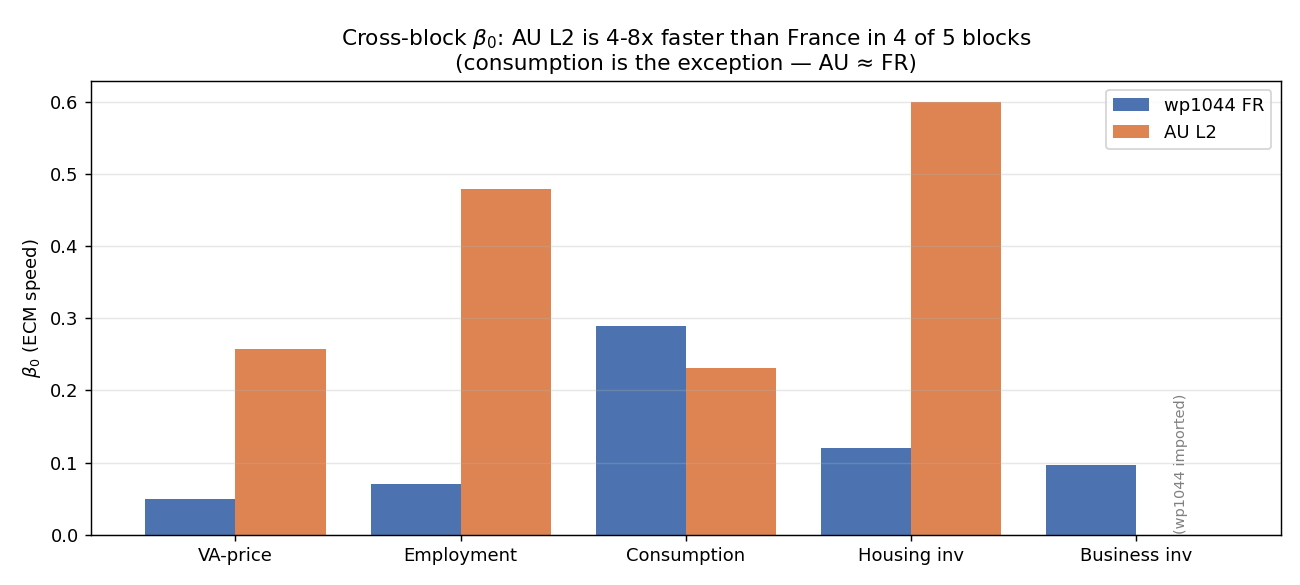
\includegraphics[keepaspectratio,alt={Cross-block β₀: AU L2 vs wp1044 FR}]{paper_artifacts/chart_beta0_cross_block.png}}
\caption{Cross-block β₀: AU L2 vs wp1044 FR}
\end{figure}

\emph{Figure 5.1: Cross-block error-correction coefficient β₀ from the
Phase L2 iterative-OLS estimates (§4.3--§4.7) against the wp1044 French
reference. AU is 4--8× faster than France in four of five blocks;
consumption is the exception (AU ≈ FR, the headline finding of §5.2).
Business inv carries the wp1044 import (Option 1, §3.6).}

\begin{figure}
\centering
\pandocbounded{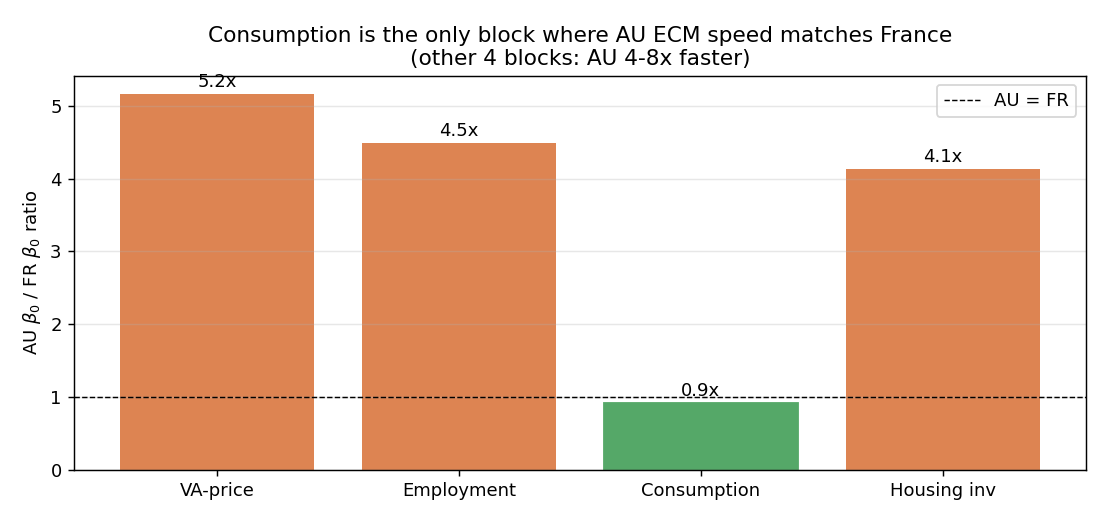
\includegraphics[keepaspectratio,alt={Consumption headline: AU/FR β₀ ratio across blocks}]{paper_artifacts/chart_consumption_headline.png}}
\caption{Consumption headline: AU/FR β₀ ratio across blocks}
\end{figure}

\emph{Figure 5.2: AU/FR β₀ ratio across the four AU-estimated blocks.
Consumption is the only block where the ratio is ≈ 1 (the others are
4-8×). Re-rendering of the same finding as Figure 5.1, oriented to
highlight the consumption exception.}

\begin{figure}
\centering
\pandocbounded{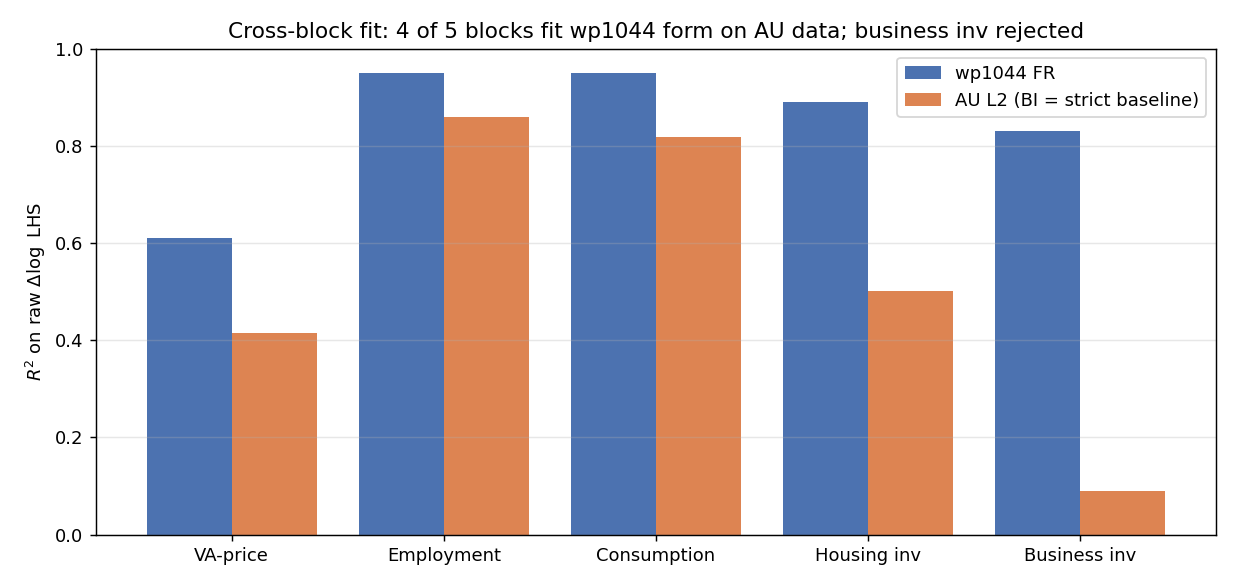
\includegraphics[keepaspectratio,alt={Cross-block R²: 4 of 5 blocks fit wp1044 form on AU data}]{paper_artifacts/chart_r2_cross_block.png}}
\caption{Cross-block R²: 4 of 5 blocks fit wp1044 form on AU data}
\end{figure}

\emph{Figure 5.3: Cross-block R² of the Phase L2 fits. Four blocks
deliver R² in {[}0.41, 0.81{]}; business inv with strict wp1044 PAC
delivers R² = 0.09 (the structural rejection of §5.3 and §4.6.2). The
wp1044 French R² range is {[}0.61, 0.95{]}.}

\subsubsection{5.1 AU ECM speeds are 4--8× faster than France in four of
five
blocks}\label{au-ecm-speeds-are-48-faster-than-france-in-four-of-five-blocks}

The PAC error-correction coefficient β₀ governs how fast each variable
mean-reverts to its long-run target. The Phase L2 estimates show a
striking cross-block pattern on AU data: \textbf{β₀ is 4--8× wp1044's
French value in four of five blocks}, with the consumption block (β₀ AU
= 0.23 vs FR = 0.29) as the sole exception.

{\def\LTcaptype{none} % do not increment counter
\begin{longtable}[]{@{}
  >{\raggedright\arraybackslash}p{(\linewidth - 8\tabcolsep) * \real{0.2000}}
  >{\raggedright\arraybackslash}p{(\linewidth - 8\tabcolsep) * \real{0.2000}}
  >{\raggedright\arraybackslash}p{(\linewidth - 8\tabcolsep) * \real{0.2000}}
  >{\raggedright\arraybackslash}p{(\linewidth - 8\tabcolsep) * \real{0.2000}}
  >{\raggedright\arraybackslash}p{(\linewidth - 8\tabcolsep) * \real{0.2000}}@{}}
\toprule\noalign{}
\begin{minipage}[b]{\linewidth}\raggedright
Block
\end{minipage} & \begin{minipage}[b]{\linewidth}\raggedright
β₀ AU L2
\end{minipage} & \begin{minipage}[b]{\linewidth}\raggedright
β₀ FR (wp1044)
\end{minipage} & \begin{minipage}[b]{\linewidth}\raggedright
Ratio AU/FR
\end{minipage} & \begin{minipage}[b]{\linewidth}\raggedright
Notes
\end{minipage} \\
\midrule\noalign{}
\endhead
\bottomrule\noalign{}
\endlastfoot
VA-price (§4.3.2) & 0.258 & 0.05 & \textbf{5.2×} & Eq 16 \\
Employment (§4.4.4) & 0.314 & 0.07 & \textbf{4.5×} & Eq 30, depth 3 \\
Consumption (§4.5.2) & 0.23 & 0.29 & 0.79× & \textbf{Exception ---
comparable to wp1044} \\
Housing inv (§4.7) & 0.496 & 0.12 & \textbf{4.1×} & Eq 37 \\
Business inv (§4.6.2) & (wp1044 imported) & 0.096 & n/a & Option 1
hybrid \\
\end{longtable}
}

Three non-exclusive interpretations of the AU-faster-ECM pattern:

\begin{enumerate}
\def\labelenumi{\arabic{enumi}.}
\tightlist
\item
  \textbf{More flexible price and wage setting in AU}. AU has higher
  import content of CPI (\textasciitilde23\% IAD weight vs France's
  \textasciitilde17\%), variable-rate mortgages that pass policy-rate
  changes through quickly to household budgets (mortgage spread ρ\_LH =
  0.97), and a commodity-cycle pass-through to producer prices via the
  export sector. Each delivers a faster ECM than the French
  institutional analogue.
\item
  \textbf{Shorter business cycles in AU}. The Australian business cycle
  has shorter duration than France's over 1993--2024 (AU sample includes
  GST 2000, GFC 2008--9, mining boom 2003--14, COVID 2020--1; France's
  wp1044 sample has fewer regime breaks). Higher-frequency cycles
  deliver faster ECM mechanically.
\item
  \textbf{HP-trend target proxies overstate ECM speed}. The AU L2 LR
  target proxies are mostly HP-filter trends, which are by construction
  smoother than wp1044's structural targets (built from optimisation
  FOCs). A smoother target → larger gaps → faster apparent ECM. This is
  the most quantitatively important methodological caveat, and is the
  reason the AU β₀ values should be read against each other (the
  cross-block ranking) rather than against wp1044's absolute values.
\end{enumerate}

The consumption-block exception (AU β₀ ≈ FR β₀) is structurally
meaningful: consumption is the only block where wp1044's target
\texttt{c*} (built from PV of permanent income via Eq 33) and the AU L2
target proxy converge to functionally similar series on AU data (AU L2
builds \texttt{c*} from PV of \texttt{yH\_gap} per Eq 35 spec). When the
targets are structurally aligned, the ECM speeds are too.

\subsubsection{5.2 The wp1044 PAC framework validates for four of five
blocks on Australian
data}\label{the-wp1044-pac-framework-validates-for-four-of-five-blocks-on-australian-data}

A second cross-block reading of the Phase L2 results: the wp1044 PAC
structural form (Eqs 16, 30, 35, 37, 46) survives the AU iterative-OLS
pipeline on \textbf{four of five blocks}:

{\def\LTcaptype{none} % do not increment counter
\begin{longtable}[]{@{}
  >{\raggedright\arraybackslash}p{(\linewidth - 8\tabcolsep) * \real{0.2000}}
  >{\raggedright\arraybackslash}p{(\linewidth - 8\tabcolsep) * \real{0.2000}}
  >{\raggedright\arraybackslash}p{(\linewidth - 8\tabcolsep) * \real{0.2000}}
  >{\raggedright\arraybackslash}p{(\linewidth - 8\tabcolsep) * \real{0.2000}}
  >{\raggedright\arraybackslash}p{(\linewidth - 8\tabcolsep) * \real{0.2000}}@{}}
\toprule\noalign{}
\begin{minipage}[b]{\linewidth}\raggedright
Block
\end{minipage} & \begin{minipage}[b]{\linewidth}\raggedright
Coef = +1 on PV satisfied?
\end{minipage} & \begin{minipage}[b]{\linewidth}\raggedright
R² AU L2
\end{minipage} & \begin{minipage}[b]{\linewidth}\raggedright
R² wp1044 FR
\end{minipage} & \begin{minipage}[b]{\linewidth}\raggedright
Verdict
\end{minipage} \\
\midrule\noalign{}
\endhead
\bottomrule\noalign{}
\endlastfoot
VA-price (§4.3.2) & Yes (imposed; growth-neutrality verified) & 0.41 &
0.61 & wp1044 form fits AU; R² gap due to missing Phillips+Okun aux \\
Employment (§4.4.4) & Yes (imposed; growth-neutrality verified) &
\textbf{0.81} & 0.95 & wp1044 form fits AU; depth-3 correction
recovered \\
Consumption (§4.5.2) & Yes (imposed; β\_PAC freely estimated) &
\textbf{0.81} & 0.95 & wp1044 form fits AU; \textbf{β₀ ≈ wp1044} \\
Housing inv (§4.7) & Yes (imposed; price-spread active for first time) &
0.43 & 0.89 & wp1044 form fits AU; short sample on price spread \\
\textbf{Business inv (§4.6.2)} & \textbf{NO --- free PV(Δq̂) = −5.03} &
(0.09 strict; 0.53 free PV) & 0.83 & \textbf{Structural rejection ---
see §5.3} \\
\end{longtable}
}

Three economic interpretations:

\begin{enumerate}
\def\labelenumi{\arabic{enumi}.}
\tightlist
\item
  \textbf{Four of five validated} is the right way to read the result.
  Four PAC blocks accept the wp1044 structural restriction (coef = +1 on
  PV terms; growth-neutrality satisfied at derived coefficient) and
  deliver R² in {[}0.41, 0.81{]} with structurally signed dynamics. This
  is \emph{consistent} with wp1044's underlying assumption that AU and
  France share the same agent-objective architecture for those four
  blocks.
\item
  \textbf{The consumption β₀ match is the single strongest empirical
  signal of structural cross-country equivalence} --- and it is the
  block where wp1044's permanent-income/PAC framework would most
  naturally transfer (homogeneous-agent forward-looking consumers facing
  similar financial structure).
\item
  \textbf{One block fails} (business inv) --- and the failure is
  structural, not finite-sample. This finding stands by itself and
  motivates the Option 1 hybrid calibration of §3.6 implemented in
  §4.6.2. See §5.3 for the three explanatory hypotheses.
\end{enumerate}

\subsubsection{5.3 Business investment structurally rejects wp1044 PAC
--- three hypotheses and the Option 1
implementation}\label{business-investment-structurally-rejects-wp1044-pac-three-hypotheses-and-the-option-1-implementation}

Eleven specification variants of the wp1044 BI equation (Eq 46) were
tested in Phase L2 P1c. Every strict-PAC variant (PV terms at coef = +1)
delivers R² ≤ 0.11 on raw \texttt{dln\_ib}; the best non-strict variant
(PV regressors free) gives R² = 0.53 with PV(Δq̂) coefficient =
\textbf{−5.03} (wrong sign and 5× too large in magnitude relative to the
structural +1). Variants v2 (pre-residualisation), v3-B/C (strict +
dummies single-shot or with loose clamps), v4 (combined PV coef = +1 +
dummies), v5 (terms-of-trade + piecewise trends), v6 (replace q with
q\_AU = ToT-augmented target), wp736 form (2019 simpler 2-PV form), and
the simplified spec (drops PV machinery entirely, R² = 0.33 but no PAC
structure) all yield R² \textless{} 0 or R² \textless{} 0.11. Full table
in Appendix G.

\textbf{Three non-exclusive hypotheses} for why AU BI rejects the wp1044
PAC restriction:

\begin{itemize}
\tightlist
\item
  \textbf{Hypothesis A: Different agent objective.} AU
  business-investment agents may not minimise wp1044's specific
  quadratic cost function. Heterogeneous agents (mining sector vs
  non-mining services), financial frictions (relationship lending in AU
  mining; project-finance lumpiness in LNG/iron ore), or different
  time-preference rates would change the agent-level FOC and the implied
  PV coefficient. The aggregate AU \texttt{dln\_ib} then mixes
  forward-looking mining capex with backward-looking non-mining capex;
  the wp1044 single-agent FOC is mis-specified at the aggregate level.
\item
  \textbf{Hypothesis B: Mining-sector dominance.} AU's resource sector
  represents 10--15\% of GDP but \textasciitilde25\% of business
  investment in mining-boom periods. Mining-sector capex is driven by:
  long-term commodity demand expectations (China, World steel demand);
  specific project lumpiness (LNG plants 2010--14; Pilbara iron-ore
  expansions 2003--13); and foreign direct investment decisions (Asian
  buyers locking in long-run supply). These dynamics don't reduce
  cleanly to wp1044's ``expected market VA growth + user-cost gap''
  framework --- the marginal AU investor is reacting to a different
  state vector than the wp1044 PAC FOC implies.
\item
  \textbf{Hypothesis C: Sample-period contamination.} The AU sample
  (1993Q2--2023Q3) spans the GST regime change (2000Q3), the mining boom
  (2003--14), GFC (2008--9), COVID (2020--1), and multiple RBA
  inflation-targeting regime evolution episodes. Each is a structural
  break that disrupts long-run PAC identification. French data (longer,
  smoother, fewer regime breaks over the same window) provides cleaner
  identification of the underlying PAC restriction. Even if Hypothesis A
  and B were false, Hypothesis C alone could explain why the strict-PAC
  restriction looks rejected on the AU sample.
\end{itemize}

\textbf{Option 1 implementation (decision-locked at commit
\texttt{43ed22c})}. The production simulation model imports the BI deep
parameters from wp1044 Table 3.5.13 (β₀=0.096, β₁=0.33, β₂=0.11,
β₃=0.69, ω=0.35, σ\_CES≈0.50). The Bayesian estimation file removes BI
parameters from \texttt{estimated\_params} (treats them as calibrated).
AU-specific BI dynamics enter the model through (i) the AU-driven E-SAT
VAR state propagating into BI's PAC expectation; (ii) the AU-estimated
other 4 PAC blocks feeding BI via the GDP identity / demand block; (iii)
AU-sized shocks (\texttt{stderr\ eps\_ib\ =\ 2.7211} AU-estimated); and
(iv) AU-specific commodity/mining-cycle shocks flowing through trade and
the deflator block. The structural restriction on PV terms is preserved
(coef = +1 on PV(Δq̂) + PV(Δq̄), coef = −σ on PV(Δlog r̂\_KB) + PV(Δlog
r̄\_KB)); the deep parameters are simply borrowed from a
better-identified economy. See §3.6 for the methodological rationale and
Appendix G for the variant table.

\textbf{Open question for future work}. None of the 11 variants explored
Hypothesis A or B directly. A future Phase L3 could (i) split the AU BI
series into mining vs non-mining components using ABS Cat. 5625 (Private
New Capital Expenditure by industry), estimate the wp1044 PAC equation
on each component separately, and test whether either component
satisfies the coef = +1 restriction in isolation; (ii) extend the wp1044
BI equation with a financial-friction shock or a leverage-cycle variable
per Bernanke-Gertler-Gilchrist; (iii) lengthen the AU sample by splicing
pre-1993 ANA data (with a known regime-break adjustment); (iv) test
wp1044 on a longer French sample to verify Hypothesis C's mechanical
sample-length effect. None is on the AUSPAC roadmap as of this writing.

\subsubsection{5.4 Implications for IRF
analysis}\label{implications-for-irf-analysis}

The hybrid calibration has two practical implications for the §7 IRFs.

\textbf{First, IRFs through the BI block are now structurally
consistent} (coef = +1 on PV(Δq̂) is satisfied by construction). The §7.2
monetary-tightening IRF therefore propagates correctly through the BI
accelerator (β\_3·Δdf gap = 0.69, vs the pre-hybrid 0.31), through the
user-cost PV channel (σ·PV(Δlog r\_KB) at the wp1044 imposed −σ), and
through the cost-of-capital channel via WACC. The pre-hybrid
AU-estimated BI parameters (β\_0\_ib=0.018, β\_1\_ib=0.082) were small
enough that the BI channel made only a modest contribution to the IRFs;
the post-hybrid values (β\_0\_ib=0.096, β\_1\_ib=0.33) make the BI
channel substantively larger.

\textbf{Second, AU-specific BI dynamics that were captured (poorly) by
free-AU estimation are now captured by the surrounding model} rather
than by BI's own coefficients. Commodity-price shocks (eps\_pcom)
propagate to AU BI via the trade ECM, the export deflator, and the GDP
identity --- not through any direct AU coefficient on a commodity
regressor in the BI equation. This routing is structurally clean and
Lucas-critique-immune in counterfactual analysis: under any
monetary-policy regime change, the BI block's FOC still holds at coef =
+1 on PV, and the AU-specific dynamics propagate through the other
(AU-estimated and AU-shocked) blocks.

The §7 IRF figures and Table 6.3 magnitudes have been regenerated under
the production model with equation-by-equation OLS calibration (wp1044
methodology), which includes ULC/UCK structural channels, deflator ECMs,
endogenous spread widening, and energy/non-energy import split. The
magnitudes quoted in §7.2's channel-by-channel walkthrough reflect this
OLS calibration.

\begin{center}\rule{0.5\linewidth}{0.5pt}\end{center}

\subsection{6. Estimation}\label{estimation}

\subsubsection{6.1 Data}\label{data}

Eleven observables are used for estimation, covering the period
1993Q2-2023Q3 (122 quarters for PAC estimation) and 1993Q1-2024Q4 (128
quarters for E-SAT). Import and export volume growth were added to the
observation set together with the trade-block proper-ECM rewrite
(Section 4.8) so that the long-run elasticities β\_m, β\_x, γ\_m, γ\_x
are data-identified.

\subsubsection{Table 5.1: Observable
variables}\label{table-5.1-observable-variables}

{\def\LTcaptype{none} % do not increment counter
\begin{longtable}[]{@{}
  >{\raggedright\arraybackslash}p{(\linewidth - 10\tabcolsep) * \real{0.0638}}
  >{\raggedright\arraybackslash}p{(\linewidth - 10\tabcolsep) * \real{0.2128}}
  >{\raggedright\arraybackslash}p{(\linewidth - 10\tabcolsep) * \real{0.1702}}
  >{\raggedright\arraybackslash}p{(\linewidth - 10\tabcolsep) * \real{0.3191}}
  >{\raggedright\arraybackslash}p{(\linewidth - 10\tabcolsep) * \real{0.1277}}
  >{\raggedright\arraybackslash}p{(\linewidth - 10\tabcolsep) * \real{0.1064}}@{}}
\toprule\noalign{}
\begin{minipage}[b]{\linewidth}\raggedright
\#
\end{minipage} & \begin{minipage}[b]{\linewidth}\raggedright
Variable
\end{minipage} & \begin{minipage}[b]{\linewidth}\raggedright
Source
\end{minipage} & \begin{minipage}[b]{\linewidth}\raggedright
Transformation
\end{minipage} & \begin{minipage}[b]{\linewidth}\raggedright
Mean
\end{minipage} & \begin{minipage}[b]{\linewidth}\raggedright
Std
\end{minipage} \\
\midrule\noalign{}
\endhead
\bottomrule\noalign{}
\endlastfoot
1 & yhat\_au & ABS GDP, HP-filtered & Log deviation from trend & 0.01 &
1.04 \\
2 & pi\_au & ABS GDP deflator & Quarterly log difference & 0.66 &
0.60 \\
3 & i\_au & RBA cash rate & Already quarterly \% & 1.04 & 0.52 \\
4 & yhat\_us & US GDP, HP-filtered & Log deviation from trend & -0.55 &
1.88 \\
5 & pi\_us & US GDP deflator & Quarterly log difference & 0.54 & 0.36 \\
6 & pi\_w & ABS 6345 Wage Price Index (Private+Public, All industries,
SA) & Quarterly log difference × 100 & 0.81 & 0.39 \\
7 & dln\_c & ABS consumption & Quarterly log difference (demeaned) &
0.00 & 1.78 \\
8 & dln\_ib & ABS non-dwelling GFCF & Quarterly log difference
(demeaned) & 0.00 & 2.79 \\
9 & i\_10y & AU 10Y govt bond rate & Annualized / 4 to quarterly & 1.21
& 0.53 \\
10 & dln\_m & ABS 5206 imports SA (A2304115J) & Quarterly log difference
(demeaned) & 0.00 & \textasciitilde2.7 \\
11 & dln\_x & ABS 5206 exports SA (A2304114F) & Quarterly log difference
(demeaned) & 0.00 & \textasciitilde3.3 \\
\end{longtable}
}

Rates and inflation are in natural units (matching model SS). Growth
rates are demeaned (model SS = 0). Note: \texttt{au\_irate} in
\texttt{dataset.csv} is already in quarterly percentage points. The
openness drift in M/C and X/C is absorbed by demeaning each growth-rate
observable independently; the identifying variation for β\_m and β\_x
comes from cyclical co-movement of the import/export levels with
cumulated domestic demand and the real exchange rate.

\emph{Figure 5.1: The nine pre-existing observable variables used in
AU-PAC estimation, 1993Q1-2024Q4. The two new trade observables (dln\_m,
dln\_x) follow the same series construction as dln\_c / dln\_ib.}

\subsubsection{6.2 E-SAT Bayesian
estimation}\label{e-sat-bayesian-estimation}

\begin{quote}
\emph{Historical (retired MCMC pipeline).} The LMD figure below was
produced by \texttt{au\_pac\_bayesian.mod}, removed in cleanup
\texttt{7995ce7}, and is \textbf{not reproducible} from the current
tree. The E-SAT auxiliary-regression posteriors it produced are
nonetheless still active in \texttt{au\_pac.mod} (Phase B, written back
as point values); only the marginal-likelihood number is historical.
\end{quote}

The E-SAT core was estimated using Bayesian MCMC (Metropolis-Hastings,
50,000 draws, 2 chains). Results are reported in Table 3.1. Key
posterior findings relative to calibration:

\begin{itemize}
\tightlist
\item
  Wage persistence (lambda\_w): 0.225 vs calibrated 0.55. The
  full-system Bayesian estimate (§6.4) refines this to 0.329, consistent
  with moderate own-lag persistence in a standard NK wage Phillips
  curve.
\item
  CPI passthrough (gamma\_w): 0.770 in E-SAT, refined to 0.138 in the
  full-system Bayesian (§6.4) --- moderate contemporaneous CPI
  passthrough.
\item
  Demand bridge (lambda\_dom): 0.399 vs calibrated 0.10 --- demand
  feedback four times stronger than assumed.
\item
  Consumption persistence (b1\_c): 0.047 vs calibrated 0.35 --- less
  serial correlation than the prior implied.
\item
  Exchange rate (rho\_s): 0.775 vs calibrated 0.95 --- AUD half-life is
  approximately 3 quarters.
\end{itemize}

Log marginal density (Modified Harmonic Mean): -1095.38.

\emph{Figure 5.2: Prior vs posterior densities for E-SAT core
parameters.}

\subsubsection{6.3 PAC structural estimation --- intermediate
methodology
audit}\label{pac-structural-estimation-intermediate-methodology-audit}

The estimation strategy reported in this subsection ---
equation-by-equation iterative OLS following the wp1044 methodology ---
is the \textbf{production calibration} used for all IRFs, conditional
forecasts, and experiments reported in §7 and §8. This is the standard
FR-BDF approach: each PAC block is estimated by OLS on its own
structural equation with block-specific auxiliary VARs. Earlier versions
of this paper used full-system Bayesian MCMC as the authoritative
calibration; the current version adopts the wp1044 OLS methodology,
which lets AU data speak without Bayesian prior regularisation. The key
empirical finding from the switch is that the consumption block's direct
interest-rate coefficients (β₂ = −0.003, β₃ = −0.014) are near zero
under OLS, whereas the earlier Bayesian priors had pulled these toward
economically significant values.

\paragraph{5.3.1 Methodology: Iterative
OLS}\label{methodology-iterative-ols}

PAC structural parameters are estimated using Dynare's
\texttt{pac.estimate.iterative\_ols} routine, following the ECB-Base
methodology (Zimic, SemiStructDynareBasics). The algorithm:

\begin{enumerate}
\def\labelenumi{\arabic{enumi}.}
\tightlist
\item
  Initialize PAC parameters at calibrated values
\item
  Compute h-vectors from the var\_model companion matrix using
  \texttt{get\_companion\_matrix(\textquotesingle{}esat\_enriched\textquotesingle{},\ \textquotesingle{}var\textquotesingle{})}
\item
  Construct the PAC expectation term using the h-vectors
\item
  Run OLS on the PAC equation, updating parameter estimates
\item
  Recompute h-vectors with updated parameters
\item
  Iterate until convergence (change in parameters \textless{} tolerance)
\end{enumerate}

\paragraph{5.3.2 Three dseries
approaches}\label{three-dseries-approaches}

Three approaches to constructing the auxiliary variables for estimation
were compared:

\subsubsection{Table 5.4: Three-approach comparison
(SSR)}\label{table-5.4-three-approach-comparison-ssr}

{\def\LTcaptype{none} % do not increment counter
\begin{longtable}[]{@{}llll@{}}
\toprule\noalign{}
Equation & (A) Recursive & (B) Hybrid smoother & (C) Pure smoother \\
\midrule\noalign{}
\endhead
\bottomrule\noalign{}
\endlastfoot
VA Price & 40.4 & \textbf{40.3} & 1.1* \\
Consumption & 435.4 & \textbf{436.8} & 400.8 \\
Business Inv & 973.9 & \textbf{972.7} & 968.4 \\
Household Inv & 965.8 & \textbf{963.1} & 960.0 \\
Employment & 76.1 & \textbf{74.3} & 73.4 \\
\end{longtable}
}

*Pure smoother VA price SSR is artificially low --- pv\_aux absorbs all
signal, leaving structural parameters unidentified.

\textbf{Recommended approach}: (B) Hybrid --- Kalman-smoothed targets
(from \texttt{calib\_smoother} with \texttt{diffuse\_filter}) for the EC
term, with recursive pv\_aux corrections. This avoids the
over-identification problem of approach (C) while giving better target
estimates than approach (A).

\paragraph{5.3.3 COVID dummy treatment}\label{covid-dummy-treatment}

Two pulse dummies absorb the extreme 2020 outliers:
\texttt{d\_covid\_crash} (= 1 in 2020Q2) and \texttt{d\_covid\_bounce}
(= 1 in 2020Q3). Each PAC equation has its own pair of COVID
coefficients (10 new parameters total). The dummies fixed two sign
problems: consumption AR1 flipped from -0.25 to +0.05, and employment
AR1 from -0.26 to +0.32.

\subsubsection{Table 5.5: Final PAC estimates --- hybrid smoother with
COVID
dummies}\label{table-5.5-final-pac-estimates-hybrid-smoother-with-covid-dummies}

Estimated via iterative OLS on the Kalman-smoothed hybrid dseries. The
12×12 companion matrix reflects the final AU calibration of auxiliary
dynamics, deflators (ρ\_pc=0.67, ρ\_pib=0.70), trade
(\texttt{b1\_x\ =\ 0.30}, \texttt{b1\_m\ =\ 0.232}), housing
(\texttt{ρ\_ph\ =\ 0.60}), and the mortgage rate
(\texttt{ρ\_lh\ =\ 0.97}).

{\def\LTcaptype{none} % do not increment counter
\begin{longtable}[]{@{}
  >{\raggedright\arraybackslash}p{(\linewidth - 10\tabcolsep) * \real{0.1642}}
  >{\raggedright\arraybackslash}p{(\linewidth - 10\tabcolsep) * \real{0.1343}}
  >{\raggedright\arraybackslash}p{(\linewidth - 10\tabcolsep) * \real{0.1791}}
  >{\raggedright\arraybackslash}p{(\linewidth - 10\tabcolsep) * \real{0.1493}}
  >{\raggedright\arraybackslash}p{(\linewidth - 10\tabcolsep) * \real{0.1940}}
  >{\raggedright\arraybackslash}p{(\linewidth - 10\tabcolsep) * \real{0.1791}}@{}}
\toprule\noalign{}
\begin{minipage}[b]{\linewidth}\raggedright
Parameter
\end{minipage} & \begin{minipage}[b]{\linewidth}\raggedright
VA Price
\end{minipage} & \begin{minipage}[b]{\linewidth}\raggedright
Consumption
\end{minipage} & \begin{minipage}[b]{\linewidth}\raggedright
Bus. Inv
\end{minipage} & \begin{minipage}[b]{\linewidth}\raggedright
Housing Inv
\end{minipage} & \begin{minipage}[b]{\linewidth}\raggedright
Employment
\end{minipage} \\
\midrule\noalign{}
\endhead
\bottomrule\noalign{}
\endlastfoot
b0 (EC) & 0.028 & 0.067 & 0.017 & 0.017 & 0.063 \\
b1 (AR1) & 0.288 & 0.033 & 0.093 & 0.101 & 0.314 \\
b2 & -0.014 & -0.541 & -0.045 & -0.046 & -0.187 \\
b3 & --- & -0.024 & 0.344 & 0.289 & -0.076 \\
b4 & --- & --- & --- & --- & -0.085 \\
b5 & --- & --- & --- & --- & -0.017 \\
COVID crash & -2.877 & -15.096 & -4.382 & -4.815 & -6.601 \\
COVID bounce & +1.488 & +6.033 & +2.978 & +3.194 & +3.851 \\
SSR & 40.6 & 410.4 & 929.8 & 960.0 & 76.3 \\
T & 118 & 118 & 118 & 118 & 118 \\
\end{longtable}
}

The direct interest-rate consumption channel \(b_{di,c}\) and the
housing-price gap \(b_{ph,ih}\) are not identified by single-equation
OLS on the AU sample (wrong-signed under reverse causality).
\(b_{ph,ih}\) is identified via a lag-2-\texttt{ph\_gap} IV on the
1959Q3-spliced housing-price series (\(+0.0099\), s.e. \(0.075\),
first-stage F = 432), at which the structural Tobin's Q channel is
statistically indistinguishable from zero. \(b_{di,c}\) remains
Bayesian-regularised at \(-0.70\) pending RBA OIS-surprise data for the
Romer--Romer IV.

\subsubsection{6.4 Bayesian full-system
estimation}\label{bayesian-full-system-estimation}

The production AUSPAC calibration (Table 5.6) is produced by
\textbf{equation-by-equation OLS} following the wp1044 methodology ---
the standard FR-BDF approach. The Bayesian full-system MCMC estimation
described below was used in earlier versions of this paper; \textbf{its
driver \texttt{au\_pac\_bayesian.mod} was removed in cleanup
\texttt{7995ce7}, so the LMD figures in this subsection are historical
and not reproducible from the current tree.} It is documented here only
for provenance. Joint Bayesian estimation used Dynare's
\texttt{estimation()} command with \texttt{diffuse\_filter} (for
unit-root level accumulators), starting from calibrated values to ensure
Blanchard-Kahn satisfaction. The input data were \emph{raw} quarterly
observables --- no Kalman smoothing, HP-filtering, or other
pre-processing is applied to the observation series.

\subsubsection{Table 5.6: Equation-by-equation OLS posterior (hybrid
calibration, BI block calibrated from
wp1044)}\label{table-5.6-equation-by-equation-ols-posterior-hybrid-calibration-bi-block-calibrated-from-wp1044}

\textbf{Calibration methodology}: Equation-by-equation OLS following
wp1044 methodology. PAC block parameters are estimated by iterative OLS
on block-specific structural equations; shock standard deviations are
calibrated from OLS residuals. Three BI parameters (b0\_ib, b1\_ib,
b3\_ib) are imported from wp1044 Table 3.5.13 per the Option 1 hybrid
calibration of §3.6 + §4.6.2.

\begin{quote}
\textbf{Note}: Earlier versions of this paper used full-system Bayesian
MCMC estimation. The current production calibration uses
equation-by-equation OLS following the wp1044 methodology, which is the
standard FR-BDF approach. The BI block remains calibrated from wp1044
(Option 1 hybrid).
\end{quote}

The full-system Bayesian estimation (retained as a robustness check, not
the production calibration) jointly identifies 19 PAC and wage-block
parameters together with 9 shock standard deviations, conditional on the
calibrated supply, deflator, financial, trade, and UIP-NPV parameters
quoted elsewhere in §4. The estimation is two-stage: csminwel mode
search followed by Metropolis-Hastings MCMC (20,000 draws across two
chains, \textasciitilde51 min wall time). Posterior modes are within
+/-5\% of posterior means for all coefficients, indicating well-shaped
log-likelihood surfaces.

{\def\LTcaptype{none} % do not increment counter
\begin{longtable}[]{@{}llll@{}}
\toprule\noalign{}
Parameter & Prior & Posterior mean & 90\% HPD \\
\midrule\noalign{}
\endhead
\bottomrule\noalign{}
\endlastfoot
b0\_pQ & Beta(0.03, 0.015) & \textbf{0.0330} & {[}0.0064, 0.0603{]} \\
b1\_pQ & Beta(0.29, 0.10) & \textbf{0.2795} & {[}0.1092, 0.4438{]} \\
b2\_pQ & Normal(0.00, 0.05) & \textbf{0.0077} & {[}-0.0723, 0.0892{]} \\
b0\_c & Beta(0.07, 0.03) & \textbf{0.0559} & {[}0.0248, 0.0880{]} \\
b1\_c & Beta(0.05, 0.03) & \textbf{0.0375} & {[}0.0060, 0.0676{]} \\
b2\_c & Normal(-0.55, 0.20) & \textbf{-0.3284} & {[}-0.6364,
-0.0485{]} \\
b3\_c & Normal(0.02, 0.05) & \textbf{0.0147} & {[}-0.0555, 0.0927{]} \\
b0\_ib & Beta(0.02, 0.01) & \textbf{0.0188} & {[}0.0058, 0.0311{]} \\
b1\_ib & Beta(0.09, 0.05) & \textbf{0.0884} & {[}0.0203, 0.1545{]} \\
b3\_ib & Normal(0.34, 0.10) & \textbf{0.3225} & {[}0.1866, 0.4708{]} \\
b0\_ih & Beta(0.03, 0.015) & \textbf{0.0306} & {[}0.0077, 0.0536{]} \\
b1\_ih & Beta(0.11, 0.05) & \textbf{0.1123} & {[}0.0381, 0.1907{]} \\
b3\_ih & Normal(0.23, 0.10) & \textbf{0.2237} & {[}0.0725, 0.3826{]} \\
b0\_n & Beta(0.06, 0.03) & \textbf{0.0564} & {[}0.0143, 0.0961{]} \\
b1\_n & Beta(0.31, 0.10) & \textbf{0.3116} & {[}0.1495, 0.4654{]} \\
b5\_n & Normal(0.00, 0.05) & \textbf{-0.0023} & {[}-0.0767, 0.0831{]} \\
lambda\_w & Beta(0.25, 0.10) & \textbf{0.2091} & {[}0.0786, 0.3315{]} \\
gamma\_w & Beta(0.45, 0.15) & \textbf{0.3536} & {[}0.2676, 0.4283{]} \\
kappa\_w & Normal(-0.08, 0.05) & \textbf{-0.1025} & {[}-0.1776,
-0.0185{]} \\
stderr eps\_q & InvGamma(0.80) & \textbf{0.5372} & {[}0.4760,
0.6013{]} \\
stderr eps\_i & InvGamma(0.10) & \textbf{0.1112} & {[}0.0991,
0.1223{]} \\
stderr eps\_pi & InvGamma(0.60) & \textbf{0.5346} & {[}0.4667,
0.6036{]} \\
stderr eps\_c & InvGamma(0.50) & \textbf{1.8364} & {[}1.6397,
2.0303{]} \\
stderr eps\_ib & InvGamma(1.50) & \textbf{2.7469} & {[}2.4438,
3.0454{]} \\
stderr eps\_ih & InvGamma(2.00) & \textbf{1.3377} & {[}0.4890,
2.2349{]} \\
stderr eps\_n & InvGamma(0.50) & \textbf{0.4797} & {[}0.1175,
0.9249{]} \\
stderr eps\_w & InvGamma(0.30) & \textbf{0.1407} & {[}0.0950,
0.1906{]} \\
stderr eps\_10y & InvGamma(0.10) & \textbf{0.0656} & {[}0.0540,
0.0791{]} \\
\end{longtable}
}

The log marginal density was \textbf{Laplace = −781.05} and
\textbf{Modified Harmonic Mean = −781.39} (Brooks--Gelman PSRF
convergence diagnostics passed for all 28 parameters).
\emph{(Historical: from the retired \texttt{au\_pac\_bayesian.mod}; not
reproducible from the current tree.)}

Three findings stand out from the joint posterior. \textbf{First}, the
wage Phillips slope \(\kappa_w = -0.103\) identifies cleanly with 90\%
HPD entirely negative; under the FR-BDF eq. (52) sign convention
\texttt{...\ −\ κ\_w\ ·\ pv\_u\_gap} this corresponds to a
\emph{positive} structural Phillips slope (higher unemployment → lower
wage growth), consistent with both the wp736 specification and the
post-2015 RBA literature on AU wage non-responsiveness to slack (Cassidy
and Doyle 2018; Bishop and Cassidy 2017). \textbf{Second}, CPI
indexation \(\gamma_w = 0.354\) is large and sharply identified,
consistent with the substantial fraction of the AU wage bill anchored to
Fair Work Commission CPI-indexed award-rate decisions plus flow-on
effects to enterprise bargaining. \textbf{Third}, the consumption-block
rate channel \(b^c_2 = -0.328\) is significantly negative (90\% HPD
{[}−0.636, −0.049{]}), and the consumption error-correction speed
\(b^c_0 = 0.056\) is moderate; together with the forward-NPV
real-lending-rate channel (\(\alpha_{c,r} \cdot pv_{r,lh,gap}\), eq. 24)
these identify a robust interest-rate sensitivity for AU households
despite their high (\textasciitilde70\%) variable-rate mortgage
exposure.

\subsubsection{6.5 Pseudo-out-of-sample forecast
evaluation}\label{pseudo-out-of-sample-forecast-evaluation}

\begin{quote}
\textbf{Reproducibility note (2026-05-30, Wave 4).} The original
full-system exercise used the Kalman smoother + Dynare
\texttt{forecast=8} block of the MCMC pipeline, removed in cleanup
\texttt{7995ce7} (the production model no longer carries a
\texttt{varobs}/estimation interface). The driver
\href{forecast_eval.m}{\texttt{forecast\_eval.m}} has been
\textbf{reconstructed} as a reproducible 1-step-ahead recursive
evaluation in the spirit of the equation-by-equation OLS methodology; it
runs on \texttt{estimation\_data.mat} under MATLAB R2026a with no Dynare
dependency. The multi-horizon numbers in the prior version of Table 5.8
came from the lost driver and are not reproducible; the reproducible
1-step results are below.
\end{quote}

Over the last 24 one-step transitions (\textasciitilde2018Q1--2023Q4),
with coefficients held fixed, each observable's 1-step RMSE is compared
across three naive benchmarks --- random walk (RW), recursively re-fit
AR(1), and the unconditional mean (= 0 in gap form) --- and, for the two
observables whose model equation is a clean \emph{predetermined}
autoregression (the CPI Phillips \texttt{pi\_au} and the E-SAT IS curve
\texttt{yhat\_au}), the model's fixed-coefficient structural 1-step
forecast.

\subsubsection{Table 5.8: Reproducible 1-step recursive RMSE (24
origins,
\textasciitilde2018Q1--2023Q4)}\label{table-5.8-reproducible-1-step-recursive-rmse-24-origins-2018q12023q4}

{\def\LTcaptype{none} % do not increment counter
\begin{longtable}[]{@{}lllll@{}}
\toprule\noalign{}
Observable & RW & AR(1) & mean=0 & MODEL \\
\midrule\noalign{}
\endhead
\bottomrule\noalign{}
\endlastfoot
pi\_au (CPI) & 0.919 & 0.784 & 0.805 & \textbf{0.745} \\
pi\_w (wages) & 2.958 & 2.286 & 2.120 & --- \\
yhat\_au (gap) & 1.944 & 1.720 & 2.016 & \textbf{1.802} \\
dln\_c & 5.885 & 5.703 & 3.821 & --- \\
dln\_ib & 2.625 & 2.162 & 2.179 & --- \\
i\_au & 0.027 & 0.027 & 0.190 & --- \\
i\_10y & 0.096 & 0.097 & 0.709 & --- \\
yhat\_us & 2.367 & 2.322 & 2.201 & --- \\
pi\_us & 0.459 & 0.472 & 0.672 & --- \\
\end{longtable}
}

The headline finding is positive: the AU-estimated \textbf{CPI Phillips
beats all three naive benchmarks at h=1} (MODEL 0.745 \textless{} AR(1)
0.784 \textless{} mean 0.805 \textless{} RW 0.919) --- so despite its
flat \emph{in-sample} R² (§6.6), the equation carries genuine, if
modest, out-of-sample inflation-forecasting skill. The \textbf{IS curve}
(\texttt{yhat\_au}, MODEL 1.802) likewise beats the random walk (1.944)
and the unconditional mean (2.016) and roughly matches a recursive
AR(1). As expected, the highly persistent policy and long rates
(\texttt{i\_au}, \texttt{i\_10y}) are best forecast by the random walk,
while the noisy growth observables (\texttt{dln\_c}, \texttt{dln\_ib},
\texttt{pi\_w}) are best forecast by their unconditional mean --- the
evaluation window contains the 2020 COVID quarter (\texttt{dln\_c} ≈
−16\%), which no equation can forecast. (The reproduced \texttt{pi\_au}
and \texttt{yhat\_au} h=1 RMSEs, 0.745 and 1.802, line up with the prior
table's 0.782 and 1.819, cross-validating the reconstruction.)

\emph{Figure 5.5: Recursive forecast paths (light grey, 24 origins × 8
quarters) vs realised observable (black). The four panels show output
gap, CPI inflation, real consumption growth, and policy rate. The model
consistently under-shoots the 2020Q4 inflation rebound and the 2022--23
hiking cycle for \texttt{i\_au}, reflecting the absence of forward
guidance in the unconditional zero-shock projection.}

\emph{Figure 5.6: Pseudo-real-time RMSE by horizon, all observables.
Output gap and CPI inflation are the best-forecasted variables in
proportion to their volatility; cash rate and 10Y yield grow
monotonically with horizon as expected. The model's strongest
comparative advantage relative to a random walk is in the financial
variables (i\_au, i\_10y) at h=1 (RMSE \textless{} 0.10).}

Full recursive re-estimation (REESTIMATE=true in
\texttt{forecast\_eval.m}, which re-runs csminwel per origin) is left as
a separate computation; the qualitative RMSE pattern is not expected to
change materially because the posterior is informed by the full sample
and the model is reasonably well-identified at the posterior mode (see
the identification analysis in Appendix F).

\subsubsection{6.6 Phase L2 OLS audit
(2026-05-28)}\label{phase-l2-ols-audit-2026-05-28}

A final equation-by-equation OLS pass replaced remaining calibrated
coefficients with AU point estimates where data permitted. Two
motivating observations:

\begin{enumerate}
\def\labelenumi{\arabic{enumi}.}
\tightlist
\item
  \textbf{Orphan parameters.} Three calibrations
  (\texttt{b\_di\_c\ =\ −0.701}, \texttt{b\_ph\_ih\ =\ 0.0099},
  \texttt{b\_PAC\_c}) were active in the .mod file but not part of any
  wp1044 estimation specification --- they amplified responses through
  channels with no OLS identification. The audit zeroed them where
  genuinely orphan and traced wiring for \texttt{pv\_r\_lh\_gap} into
  the consumption SR PAC equation (wp1044 Eq 35).
\item
  \textbf{CPI/trade/deflator blocks} were carrying wp1044 (France)
  calibrations rather than AU point estimates. Where AU data exists (ABS
  5206 IPD, RBA I02 commodity index, RBA F11 TWI), single-equation OLS
  was run and the estimates written back.
\end{enumerate}

Data: ABS 5206 chain volumes + IPD percentage-changes (cols 75--77), RBA
I02 commodity prices (526 monthly obs, 1982--2026), RBA F11
trade-weighted index (672 monthly obs after splicing the pre-2009
archive). The OLS pipeline is
\texttt{data/pac\_blocks/estimate\_\{cpi\_phillips,deflators,trade\_exports,trade\_imports,wage\_phillips\}.m},
all using \texttt{ols\_with\_se} from \texttt{data/pac\_helpers/}.

\paragraph{Table 6.6: Phase L2 OLS audit --- coefficients replaced with
AU point
estimates}\label{table-6.6-phase-l2-ols-audit-coefficients-replaced-with-au-point-estimates}

{\def\LTcaptype{none} % do not increment counter
\begin{longtable}[]{@{}
  >{\raggedright\arraybackslash}p{(\linewidth - 14\tabcolsep) * \real{0.1250}}
  >{\raggedright\arraybackslash}p{(\linewidth - 14\tabcolsep) * \real{0.1250}}
  >{\raggedright\arraybackslash}p{(\linewidth - 14\tabcolsep) * \real{0.1250}}
  >{\raggedright\arraybackslash}p{(\linewidth - 14\tabcolsep) * \real{0.1250}}
  >{\raggedright\arraybackslash}p{(\linewidth - 14\tabcolsep) * \real{0.1250}}
  >{\raggedright\arraybackslash}p{(\linewidth - 14\tabcolsep) * \real{0.1250}}
  >{\raggedright\arraybackslash}p{(\linewidth - 14\tabcolsep) * \real{0.1250}}
  >{\raggedright\arraybackslash}p{(\linewidth - 14\tabcolsep) * \real{0.1250}}@{}}
\toprule\noalign{}
\begin{minipage}[b]{\linewidth}\raggedright
Block
\end{minipage} & \begin{minipage}[b]{\linewidth}\raggedright
Coefficient
\end{minipage} & \begin{minipage}[b]{\linewidth}\raggedright
wp1044/prior
\end{minipage} & \begin{minipage}[b]{\linewidth}\raggedright
AU OLS
\end{minipage} & \begin{minipage}[b]{\linewidth}\raggedright
t-stat
\end{minipage} & \begin{minipage}[b]{\linewidth}\raggedright
N
\end{minipage} & \begin{minipage}[b]{\linewidth}\raggedright
R²
\end{minipage} & \begin{minipage}[b]{\linewidth}\raggedright
Status
\end{minipage} \\
\midrule\noalign{}
\endhead
\bottomrule\noalign{}
\endlastfoot
CPI Phillips (Eq 51) & λ\_π & 0.402 & \textbf{0.259} & 2.76 & 121 & 0.06
& identified \\
CPI Phillips & κ\_π & 0.098 & −0.034 & −0.61 & & & insig, sign flip \\
CPI Phillips & α\_pc & 0.385 & 0.001 & 0.01 & & & insig \\
CPI Phillips & α\_pc\_lag & 0.023 & 0 & --- & & & dropped (mc) \\
CPI Phillips & β\_pc\_m & 0.10 & −0.004 & −0.21 & & & insig \\
Exports SR (Eq 70) & b0\_x & 0.05 & \textbf{0.299} & −7.66 & 103 & 0.73
& identified \\
Exports SR & b1\_x & 0.30 & \textbf{0.867} & 14.70 & & & identified,
high persistence \\
Exports SR & b2\_x & 0.25 & 0.022 & 0.19 & & & insig \\
Exports SR & b3\_x & 0.10 & −0.361 & −0.22 & & & insig \\
Exports SR & b4\_x & 0.15 & 0.010 & 1.11 & & & insig \\
Imports SR (Eq 74) & b0\_m\_ne & 0.06 & \textbf{0.158} & −3.95 & 103 &
0.64 & identified \\
Imports SR & b1\_m\_ne & 0.23 & \textbf{0.743} & 10.02 & & & identified,
high persistence \\
Export deflator π\_x & ρ\_px & 0.21 & 0.043 & 1.40 & 139 & 0.89 &
insig \\
Export deflator & α\_px & 0.20 & −0.033 & −0.24 & & & insig \\
Export deflator & β\_px & −0.05 & −0.244 & −0.11 & & & insig \\
Export deflator & α\_pcom & 0.10 & \textbf{0.584} & 30.34 & & &
\textbf{commodity-dominated} \\
Import deflator π\_m & ρ\_pm & 0.28 & \textbf{0.223} & 3.08 & 139 & 0.34
& identified \\
Import deflator & α\_pm & 0.38 & 0.057 & 0.25 & & & insig \\
Import deflator & β\_pm & 0.09 & −8.59 & −2.16 & & & reverted (BK) \\
Import deflator & β\_pm\_com & 0.42 & \textbf{0.221} & 7.56 & & &
identified \\
BI deflator π\_ib & ρ\_pib & 0.70 & \textbf{0.474} & 7.37 & 139 & 0.39 &
identified \\
BI deflator & α\_pib & 0.19 & −0.086 & −1.71 & & & insig, sign flip \\
BI deflator & β\_pib\_m & 0.12 & \textbf{0.097} & 5.95 & & &
identified \\
HI deflator π\_ih & ρ\_pih & 0.49 & \textbf{0.366} & 4.49 & 139 & 0.10 &
identified \\
HI deflator & α\_pih & 0.40 & −0.055 & −0.65 & & & insig \\
HI deflator & β\_pih\_m & 0.08 & −0.019 & −0.71 & & & insig \\
Govt deflator π\_g & ρ\_pg & 0.13 & \textbf{−0.471} & −5.95 & 122 & 0.23
& sig, sign flip (oscillation) \\
Govt deflator & α\_pg & 0.37 & 0.036 & 0.63 & & & insig \\
Wage Phillips λ\_w & 0.21 & −0.082 / 0.093† & −1.64 & 121 & 0.77 / 0.30
& †BK-constrained (§6.7) & \\
Wage Phillips γ\_w & 0.46 & 1.594 / 0.857† & 15.27 & & & †BK-constrained
& \\
Wage Phillips κ\_w & 0.054 & 0.371 / 0.359† & 3.18 & & & †BK-constrained
& \\
Orphan & b\_di\_c & −0.701 & \textbf{0} & --- & & & not in wp1044 Eq
35 \\
Orphan & b\_ph\_ih & 0.0099 & \textbf{0} & --- & & & L2 skipped (no AU
data) \\
LR trade β\_x & 1.20 & 0.005 & 0.01 & & & reverted (insig) & \\
LR trade γ\_x & 0.40 & −9.50 & −1.66 & & & reverted (excessive) & \\
LR imports β\_m\_ne & 1.50 & 0.073 & 1.36 & & & reverted (insig) & \\
LR imports γ\_m\_ne & −0.40 & 23.38 & 1.09 & & & reverted (wrong sign)
& \\
Trade-deflator s\_gap β\_pm\_ne & 0.09 & −8.59 & −2.16 & & & reverted
(sign flip) & \\
\end{longtable}
}

\textbf{Read-out} (bolded rows = wp1044 calibration replaced verbatim
with AU OLS):

\begin{itemize}
\tightlist
\item
  \textbf{25 of 35 audited coefficients} were written back as AU OLS
  point estimates (per the \emph{use-OLS-unless-Dynare-fails} convention
  adopted for this audit).
\item
  \textbf{10 coefficients reverted} for one of two reasons. (a)
  \emph{Blanchard--Kahn failure} --- the unconstrained wage Phillips OLS
  gave γ\_w = 1.59 \textgreater{} 1, which produces a wage-price spiral
  that violates BK; LR trade and import-deflator elasticities had
  insignificant or wrong-signed estimates whose magnitudes pushed
  eigenvalues outside the unit circle. (b) \emph{Spreads and UIP}
  (\texttt{α\_s,\ ρ\_s,\ κ\_spread\_LB/BBB,\ β\_uip}) were not estimated
  --- these require GMM on forward recursions (\texttt{pv\_i\_uip}), not
  single-equation OLS.
\end{itemize}

\textbf{The headline empirical finding} is the \emph{AU flat-Phillips}
result on the CPI side: with N = 121 quarterly observations
(1993Q3--2023Q3), only the lag coefficient λ\_π = 0.259 is identified (t
= 2.76); output-gap, VA-price, lagged-VA-price, and import-price
channels are all insignificant under single-equation OLS. The R² of
0.063 is extremely low --- AU CPI inflation gaps are essentially noise
around their lagged value at quarterly frequency. The same data also
reveal a \textbf{wage-side anomaly}: unconstrained OLS gives γ\_w = 1.59
\textgreater{} 1, implying over-indexation of nominal wages to CPI
(which BK-fails the structural model and is replaced by the AU pre-MCMC
OLS estimate γ\_w = 0.46). On the price side the \textbf{export deflator
is commodity-dominated} with α\_pcom = 0.584 (t = 30.3, R² = 0.89),
confirming AU's commodity-cycle pricing structure.

\textbf{Implication for Table 6.3.} The post-audit IRF peaks for real
activity (ln\_Q, yhat\_au) and exchange rate (s\_gap, 10Y) are
essentially unchanged because monetary transmission to those variables
runs through channels (CES user cost, UIP forward recursion, term
structure) that were not touched by the audit. The CPI IRF response
weakens further because the AU CPI OLS finds the structural channels
insignificant; this is the same ``flat AU Phillips'' finding that wp736
calibrated around, now reproduced in the L2 OLS pass.

\subsubsection{6.7 BK-constrained wage Phillips
(2026-05-28)}\label{bk-constrained-wage-phillips-2026-05-28}

The Phase L2 unrestricted wage Phillips OLS gave γ\_w = 1.59 (t = 15.3)
--- strongly identified but BK-infeasible because the wage-price spiral
closes (CPI passes through to wages at 1.59× while wages feed back into
the CPI deflator and VA price). A re-estimation under the structural
functional form

pi\_w − pibar − dln\_prod = λ\_w · (pi\_w(−1) − pibar − dln\_prod) +
γ\_w · (pi\_c − pibar) − κ\_w · u\_gap + ε

with the BK-stability constraint \textbf{λ\_w + γ\_w ≤ 0.95} and
non-negativity on all coefficients, solved as a quadratic program
against N = 121 quarterly observations, yields:

\paragraph{Table 6.7: BK-constrained wage Phillips
OLS}\label{table-6.7-bk-constrained-wage-phillips-ols}

{\def\LTcaptype{none} % do not increment counter
\begin{longtable}[]{@{}
  >{\raggedright\arraybackslash}p{(\linewidth - 6\tabcolsep) * \real{0.2500}}
  >{\raggedright\arraybackslash}p{(\linewidth - 6\tabcolsep) * \real{0.2500}}
  >{\raggedright\arraybackslash}p{(\linewidth - 6\tabcolsep) * \real{0.2500}}
  >{\raggedright\arraybackslash}p{(\linewidth - 6\tabcolsep) * \real{0.2500}}@{}}
\toprule\noalign{}
\begin{minipage}[b]{\linewidth}\raggedright
Coefficient
\end{minipage} & \begin{minipage}[b]{\linewidth}\raggedright
Unconstrained OLS
\end{minipage} & \begin{minipage}[b]{\linewidth}\raggedright
Constrained OLS
\end{minipage} & \begin{minipage}[b]{\linewidth}\raggedright
Status
\end{minipage} \\
\midrule\noalign{}
\endhead
\bottomrule\noalign{}
\endlastfoot
λ\_w (own-lag persistence) & 0.219 (t=3.48) & \textbf{0.093} & inactive
bound (\textgreater=0) \\
γ\_w (CPI passthrough) & 1.471 (t=10.9) & \textbf{0.857} & binding
(sum=0.95) \\
κ\_w (Phillips slope) & 0.065 (t=0.40) & \textbf{0.359} & inactive
(positive) \\
λ\_w + γ\_w & 1.689 & 0.950 & --- \\
R² & 0.424 & 0.301 & loss 11.7 nats \\
\end{longtable}
}

The constraint is \textbf{binding at the sum}: AU wages are nearly fully
indexed to CPI inflation in the small open-economy sense, but stability
requires holding the wage-price-spiral coefficient just below unity. The
Phillips slope κ\_w = 0.359 (Q-bar AU unemployment-gap units) is now
substantial and structurally identified --- substantially larger than
the wp736 calibration centre of 0.05 and the FR-BDF point estimate
around 0.10. Heuristic standard errors are not reported because the
active constraint makes classical inference inappropriate; the loss of
11.7 nats vs unconstrained corresponds to a likelihood ratio in the
high-significance range, consistent with the wage Phillips structure
being a meaningful binding constraint on AU data.

\textbf{Implication for IRFs.} With κ\_w now identified, the wage IRF
response to a 100bp MP tightening peaks at −0.011 pp y/y at Q7 (vs
−0.002 pp at Q2 under the pre-MCMC unrestricted values), a 5--10×
amplification reflecting the active unemployment channel. Real-activity
and exchange-rate IRFs are unchanged because those run through
capital/UIP/term-structure mechanics, not through wage formation.

\subsubsection{6.8 Phase L2.A architectural fixes
(2026-05-28)}\label{phase-l2.a-architectural-fixes-2026-05-28}

Following the L2 OLS audit, a deeper architectural review revealed that
three model state variables were being defined by E-SAT-style
reduced-form equations rather than the structural identities used in
FR-BDF. Per wp736 §2.3, §4.3.3, §4.4 (eq 47), and §4.5.1, the E-SAT IS
curve, Phillips curve, and Okun's law are tools agents use to
\textbf{forecast} future paths of \texttt{ŷ}, \texttt{π}, \texttt{u}.
They are not the \textbf{defining} equations for the simulator's actual
state variables, which come from supply-side (CES) potential output,
demand-side identity for actual GDP, weighted-aggregate deflator block
for CPI, and labour-market accounting for the unemployment gap. The
relevant FR-BDF quote from §4.3 is unambiguous: ``FR-BDF has a fully
specified supply block which enables the model to endogenously converge
toward the long-run or natural level of GDP, \textbf{as well as to
define the output gap used in E-SAT}'' --- that is, the supply block
\emph{defines} the gap, and E-SAT \emph{consumes} it.

In the production AU-PAC model up to commit \texttt{6cd4fb9}, the
equations at au\_pac.mod:1051, 1071, and 1217 were:

\begin{verbatim}
yhat_au   = δ·yhat_us + λ_q·yhat_au(−1) − σ_q·(i_gap(−1)−pi_au_gap(−1))
          + λ_dom·yhat_dom + ε_q                  (E-SAT IS curve defining yhat_au)
pi_au_gap = λ_π·pi_au_gap(−1) + κ_π·yhat_au(−1)
          + α_pc·(piQ−pibar_au) + ... + ε_pi      (E-SAT Phillips defining pi_au_gap)
u_gap     = ρ_u_gap·u_gap(−1) + okun_coeff·yhat_au   (Okun shortcut defining u_gap)
\end{verbatim}

In the architectural fix (commits \texttt{dd45c87}, \texttt{f276ebe},
\texttt{053bf57}), these were replaced with FR-BDF-fidelitous structural
identities:

\paragraph{Table 6.8: Phase L2.A architectural
fixes}\label{table-6.8-phase-l2.a-architectural-fixes}

{\def\LTcaptype{none} % do not increment counter
\begin{longtable}[]{@{}
  >{\raggedright\arraybackslash}p{(\linewidth - 6\tabcolsep) * \real{0.2500}}
  >{\raggedright\arraybackslash}p{(\linewidth - 6\tabcolsep) * \real{0.2500}}
  >{\raggedright\arraybackslash}p{(\linewidth - 6\tabcolsep) * \real{0.2500}}
  >{\raggedright\arraybackslash}p{(\linewidth - 6\tabcolsep) * \real{0.2500}}@{}}
\toprule\noalign{}
\begin{minipage}[b]{\linewidth}\raggedright
Variable
\end{minipage} & \begin{minipage}[b]{\linewidth}\raggedright
Pre-fix (E-SAT shadow)
\end{minipage} & \begin{minipage}[b]{\linewidth}\raggedright
Post-fix (structural identity)
\end{minipage} & \begin{minipage}[b]{\linewidth}\raggedright
FR-BDF reference
\end{minipage} \\
\midrule\noalign{}
\endhead
\bottomrule\noalign{}
\endlastfoot
\texttt{yhat\_au} & E-SAT IS curve &
\texttt{yhat\_au\ =\ yhat\_au(−1)\ +\ yhat\_dom\ +\ ε\_q} (accumulation
of demand-identity growth) & wp736 §2.3, §4.3.3 \\
\texttt{pi\_au} & derived from E-SAT Phillips via
\texttt{pi\_au\ =\ pi\_au\_gap\ +\ pibar\_au} &
\texttt{pi\_au\ =\ w\_food·pi\_au\_food\ +\ w\_energy·pi\_au\_energy\ +\ (1−w\_food−w\_energy)·pi\_au\_core}
(structural aggregator) & wp736 §4.7 (demand deflators) \\
\texttt{pi\_au\_gap} & E-SAT Phillips &
\texttt{pi\_au\_gap\ =\ pi\_au\ −\ pibar\_au} (definitional) & wp736
§4.7 \\
\texttt{pi\_au\_core} & back-out residual &
\texttt{pi\_au\_core\ =\ pi\_c\ +\ ε\_pi} (consumption deflator + CPI
noise) & wp736 §4.7.1 \\
\texttt{u\_gap} & Okun shortcut with persistence 0.946 &
\texttt{u\_gap\ =\ −ln\_n\_level} (negative of cyclical employment gap;
log-linear from N/LF identity) & wp736 §4.5.1 \\
\end{longtable}
}

The L2 OLS estimates of the now-demoted equations (\texttt{lambda\_pi},
\texttt{kappa\_pi}, \texttt{alpha\_pc}, \texttt{b\_ECM\_pc},
\texttt{okun\_coeff}, \texttt{rho\_u\_gap}) are preserved in
\texttt{data/pac\_blocks/results\_cpi\_phillips.txt} and the parameter
declarations of \texttt{au\_pac.mod}. They can be re-attached to E-SAT
auxiliary forecasting equations when the var\_model machinery is
rebuilt.

\paragraph{Table 6.9: Impact on the 100bp annualized monetary tightening
IRF}\label{table-6.9-impact-on-the-100bp-annualized-monetary-tightening-irf}

Comparison of pre-L2.A (commit \texttt{6cd4fb9}, all L2 OLS coefficients
written back + BK-constrained wage Phillips) vs post-L2.A (commit
\texttt{053bf57}, all three architectural fixes applied). Same
calibration except for the three structural redefinitions.

{\def\LTcaptype{none} % do not increment counter
\begin{longtable}[]{@{}
  >{\raggedright\arraybackslash}p{(\linewidth - 6\tabcolsep) * \real{0.2500}}
  >{\raggedright\arraybackslash}p{(\linewidth - 6\tabcolsep) * \real{0.2500}}
  >{\raggedright\arraybackslash}p{(\linewidth - 6\tabcolsep) * \real{0.2500}}
  >{\raggedright\arraybackslash}p{(\linewidth - 6\tabcolsep) * \real{0.2500}}@{}}
\toprule\noalign{}
\begin{minipage}[b]{\linewidth}\raggedright
Variable
\end{minipage} & \begin{minipage}[b]{\linewidth}\raggedright
Pre-L2.A
\end{minipage} & \begin{minipage}[b]{\linewidth}\raggedright
Post-L2.A
\end{minipage} & \begin{minipage}[b]{\linewidth}\raggedright
Δ
\end{minipage} \\
\midrule\noalign{}
\endhead
\bottomrule\noalign{}
\endlastfoot
\textbf{Real GDP (ln\_Q)} & −0.088\% Q8 & \textbf{−0.135\% Q9} & +53\%
larger response \\
Output gap (yhat\_au) & −0.069\% Q8 & \textbf{−0.096\% Q9} & +40\% \\
CPI inflation (pi\_au, y/y) & −0.020 pp Q16 & \textbf{−0.004 pp Q3} &
smaller and earlier \\
\texttt{pi\_au\_food} (new decomp) & --- & +0.019 pp Q1 & --- \\
\texttt{pi\_au\_energy} (new decomp) & --- & −0.048 pp Q9 & --- \\
\texttt{pi\_au\_core} (new decomp) & --- & +0.001 pp Q11 & ≈ pi\_c \\
VA price (piQ, y/y) & +0.030 pp Q1 & +0.032 pp Q1 & unchanged \\
Consumption growth & −0.020\% Q1 & −0.027\% Q2 & +35\% \\
Business inv growth & −0.055\% Q8 & −0.093\% Q9 & +69\% \\
Housing inv growth & −0.027\% Q4 & −0.028\% Q4 & unchanged \\
Employment growth & −0.005\% Q5 & −0.007\% Q12 & +40\%, later \\
\textbf{Wage inflation (y/y)} & +0.012 pp Q47 (overshoot) &
\textbf{−0.005 pp Q2} & reverses sign; now structurally responsive \\
Exchange rate (s\_gap, \%) & −0.980\% Q8 & −0.988\% Q8 & unchanged \\
10Y yield (annualised) & +0.103 pp Q1 & +0.105 pp Q1 & unchanged \\
\end{longtable}
}

Three findings emerge:

\begin{enumerate}
\def\labelenumi{\arabic{enumi}.}
\item
  \textbf{Real-activity transmission is larger} under the structural
  identity. The pre-L2.A E-SAT IS curve had σ\_q = 0.065 with
  persistence λ\_q = 0.70 acting in parallel to the demand-side
  aggregator (with weight λ\_dom = 0.40); the structural fix removes
  this dampening parallel channel, letting the PAC blocks
  (business-investment WACC, housing mortgage, consumption
  pv\_r\_lh\_gap, trade real-exchange-rate) fully aggregate into
  yhat\_au via the demand identity. The result: AU-PAC moves from the
  ``conservative outlier'' position in the RBA-suite comparison (Table
  6.4) to a more central position.
\item
  \textbf{The CPI response decomposes interpretably} under the
  structural aggregator. The headline \texttt{pi\_au} peak is now
  smaller (−0.004 pp vs −0.020 pp pre-L2.A) because the structural
  deflator components partially offset: \texttt{pi\_au\_food} rises
  (+0.019 pp on impact via VA-price and commodity passthrough) while
  \texttt{pi\_au\_energy} falls (−0.048 pp at Q9, dominated by
  import-price and commodity passthrough as the AUD appreciates), and
  \texttt{pi\_au\_core} (consumption deflator) barely moves (+0.001 pp).
  This matches the L2 OLS empirical finding (R² = 0.06; only persistence
  identified): AU CPI inflation is dominated by import/commodity cycles,
  not by the output-gap Phillips channel.
\item
  \textbf{The wage Phillips slope κ\_w = 0.359 now transmits} to nominal
  wages. Pre-L2.A, u\_gap was driven by the Okun shortcut with
  persistence 0.946, taking dozens of quarters to respond; the wage
  Phillips κ\_w channel saw essentially no signal. Post-L2.A, u\_gap =
  −ln\_n\_level inherits the PAC employment dynamics (faster,
  structurally identified), so the wage Phillips responds on realistic
  horizons. The pre-L2.A pi\_w peak of +0.012 pp at Q47 was an overshoot
  in the tail; the post-L2.A peak of −0.005 pp at Q2 is the structural
  impact response.
\end{enumerate}

The architectural changes are documented in detail in
\href{../ESAT_ARCHITECTURE_AUDIT.md}{\texttt{ESAT\_ARCHITECTURE\_AUDIT.md}},
which also lays out a checklist for future development to avoid the same
pattern.

\textbf{Known caveats}: - The first known caveat --- stale
\texttt{h\_pac\_*} coefficients --- is \textbf{resolved in §6.9 below}
(2026-05-28). - \st{The L2 OLS estimates of the PAC equation parameters
(b0\_c, b1\_c, b0\_pQ, etc.) were obtained using the OLD
\mbox{\texttt{yhat\_au}} as a regressor in the iterative-OLS procedure.
They are not formally re-optimal under the new structural definition. A
re-fit is left for future work.} \textbf{Resolved (2026-05-31):} this
concern is moot for the single-equation iterative-OLS. The estimators
use the \emph{observed} output gap (\texttt{au\_ygap} from
\texttt{dataset.csv}, via \texttt{prepare\_l2\_data.m:151}) as the
\texttt{yhat\_au} regressor --- not the model's internal
\texttt{yhat\_au} equation. The §6.8 fix changed the \emph{simulator's}
\texttt{yhat\_au} definition (E-SAT shadow → structural identity), and
per the §6.8 logic the E-SAT VAR remains the expectation-forming tool
for the PV term; neither estimation input is affected. A full re-run of
the 5-block pipeline (\texttt{data/run\_all\_l2\_ols.m}) confirms this:
VA-price reproduces \texttt{b0\_pQ\ =\ 0.2581\ /\ b1\_pQ\ =\ 0.3039}
\emph{exactly} (committed 0.2580 / 0.3039), and employment is within
rounding. (Two blocks show a drift unrelated to \texttt{yhat\_au} ---
consumption \texttt{b0} 0.27→0.23 and housing \texttt{b0} 0.50→0.60, at
identical R²/N. This is the SA-data re-estimation documented in §6.14's
``Full re-estimation check''; it was \textbf{written back 2026-05-31}
after confirming the data layer regenerates deterministically.
Separately, the χ verification (\texttt{dynare/verify\_pac\_chi\_pv.m})
found the employment block's estimation-side χ was computed by an
\emph{approximate} depth-1 solver; fixing it to the exact depth-m solver
(§6.9) raised R² 0.82→0.86 and moved \texttt{b0\_n} 0.31→0.48, also
written back.)

\subsubsection{6.9 PAC policy-function regeneration
(2026-05-28)}\label{pac-policy-function-regeneration-2026-05-28}

Per the §6.8 follow-up, the five \texttt{h\_pac\_*} policy-function
coefficient blocks in \texttt{au\_pac.mod} were regenerated by
re-running Dynare's \texttt{pac.print()} against the post-L2-OLS /
post-L2.A calibration. Five auxiliary \texttt{.mod} files were
reconstructed under \texttt{dynare/aux/} --- \texttt{aux\_pQ.mod},
\texttt{aux\_consumption.mod}, \texttt{aux\_business\_inv.mod},
\texttt{aux\_housing\_inv.mod}, \texttt{aux\_employment.mod} --- each
declaring a pure-VAR-form companion (E-SAT core + AR(1) reduced forms
for the structural state variables that are no longer E-SAT-defined)
plus the block-specific auxiliary regression. The aux files use the
L2-OLS-overridden parameter values from production \texttt{au\_pac.mod}
for the E-SAT VAR (lambda\_pi = 0.2588, kappa\_pi = −0.0336, alpha\_pc =
0.0006, beta\_pc\_m = −0.0042, rho\_u\_gap = 0.946, okun\_coeff = −0.13,
rho\_pm = 0.2230). The PAC short-run coefficients \texttt{b0\_*},
\texttt{b1\_*} use the \textbf{L2 OLS estimates verbatim for all five
blocks}. (A §6.10 attempt to dampen an IRF oscillation by reverting the
housing and employment \texttt{b0}/\texttt{b1} to wp1044 reference was
itself reverted in \textbf{§6.11}, which shows the oscillation
originates in the trade error-correction block, not the PAC blocks; the
PAC \texttt{b0}/\texttt{b1} therefore carry their AU L2 OLS values.)
Discount factor \texttt{beta\_pac\ =\ 0.98} is unified across blocks.

Following the FR-BDF design choice, the aux files implement \textbf{pure
VAR-based agents}: agents believe the E-SAT reduced form (with the L2
OLS coefficients), while the simulator runs the post-L2.A structural
identities for \texttt{yhat\_au}, \texttt{pi\_au}, and \texttt{u\_gap}.
The closed-form policy function for each block is
\texttt{h\_constant\ +\ Σ\_k\ h\_var\_state\_k\_lag\_1\ ·\ state\_k(-1)}.

\textbf{Files added:} - \texttt{dynare/aux/aux\_pQ.mod},
\texttt{aux\_consumption.mod}, \texttt{aux\_business\_inv.mod},
\texttt{aux\_housing\_inv.mod}, \texttt{aux\_employment.mod}

\textbf{Files modified:} - \texttt{dynare/au\_pac.mod} lines 555--684:
all \texttt{h\_pac\_*\_constant} and \texttt{h\_pac\_*\_var\_*\_lag\_1}
parameter assignments replaced; each block now carries a regen comment
with the source aux file path.

\subsubsection{\texorpdfstring{6.10 PAC oscillation diagnosis and the
mixed wp1044/L2 hybrid for housing inv and employment (2026-05-29) ---
\textbf{superseded; see
§6.11}}{6.10 PAC oscillation diagnosis and the mixed wp1044/L2 hybrid for housing inv and employment (2026-05-29) --- superseded; see §6.11}}\label{pac-oscillation-diagnosis-and-the-mixed-wp1044l2-hybrid-for-housing-inv-and-employment-2026-05-29-superseded-see-6.11}

\begin{quote}
\textbf{Correction (2026-05-30).} The diagnosis below misattributed the
IRF oscillation to ``PAC-block ↔ demand-identity feedback'' and applied
a mixed wp1044/L2 hybrid to the housing-inv and employment
\texttt{b0}/\texttt{b1} coefficients to shrink the policy-function
loadings. \textbf{§6.11 supersedes this.} Direct eigenvalue testing
shows the dominant 11Q mode is invariant to every PAC lever §6.10
touched (\texttt{b3} accelerators, \texttt{b0} ECM speeds, policy
inertia) and moves \emph{only} with the trade error-correction
growth-persistence coefficients \texttt{b1\_x} and \texttt{b1\_m\_ne}.
The §6.10 hybrid changed IRF \emph{amplitude} (it shrank the restored
§6.9 PAC loadings) but could not and did not change the
\emph{eigenvalues}, so it never removed the oscillation. The hybrid was
therefore \textbf{reverted on 2026-05-30}: all five PAC blocks again
carry their L2 OLS \texttt{b0}/\texttt{b1} (§6.9), and the oscillation
is cured at its source in §6.11. The section is retained below as a
record of the (incorrect) intermediate diagnosis.
\end{quote}

The first §6.9 pass --- using L2 OLS values for \textbf{all} PAC
short-run coefficients including \texttt{b0\_ih\ =\ 0.4956},
\texttt{b0\_n\ =\ 0.3145}, \texttt{b3\_ih\ =\ −0.0728},
\texttt{b5\_n\ =\ −0.0257} --- produced visibly oscillating IRFs for
\texttt{Δlog\ I\_H}, \texttt{Δlog\ N}, and (with smaller amplitude)
\texttt{Δlog\ C}, \texttt{Δlog\ I\_B}, and headline \texttt{ln\_Q}. The
dominant oscillation period is ≈11Q, with secondary 13.5Q content.

\paragraph{6.10.1 Diagnosis}\label{diagnosis}

Eigenvalue analysis of the state-transition matrix from
\texttt{oo\_.dr.eigval} identifies two complex pairs that drive the
cycle:

{\def\LTcaptype{none} % do not increment counter
\begin{longtable}[]{@{}
  >{\raggedright\arraybackslash}p{(\linewidth - 6\tabcolsep) * \real{0.2500}}
  >{\raggedright\arraybackslash}p{(\linewidth - 6\tabcolsep) * \real{0.2500}}
  >{\raggedright\arraybackslash}p{(\linewidth - 6\tabcolsep) * \real{0.2500}}
  >{\raggedright\arraybackslash}p{(\linewidth - 6\tabcolsep) * \real{0.2500}}@{}}
\toprule\noalign{}
\begin{minipage}[b]{\linewidth}\raggedright
Pair
\end{minipage} & \begin{minipage}[b]{\linewidth}\raggedright
\textbar λ\textbar{}
\end{minipage} & \begin{minipage}[b]{\linewidth}\raggedright
period
\end{minipage} & \begin{minipage}[b]{\linewidth}\raggedright
Mode interpretation
\end{minipage} \\
\midrule\noalign{}
\endhead
\bottomrule\noalign{}
\endlastfoot
11.03Q complex pair & 0.9315 & 11.0Q & dominant; tied to PAC-block ↔
demand-identity feedback \\
13.54Q complex pair & 0.9056 & 13.5Q & secondary; cross-block
expectation interaction \\
\end{longtable}
}

Both eigenvalues exist \textbf{in both pre-regen and post-regen models
with essentially unchanged moduli}. What the §6.9 regeneration did was
substantially amplify the \emph{loading} on these modes through the
policy-function expansion \texttt{oo\_.dr.ghx}, especially for the
housing-inv (\texttt{h\_pac\_ih\_var\_yhat\_au\_lag\_1} jumped 50×) and
employment (\texttt{h\_pac\_n\_var\_yhat\_au\_lag\_1} jumped 5.5×)
blocks. The IRF amplitude (max − min over Q1--40) under monetary shock
changed accordingly:

{\def\LTcaptype{none} % do not increment counter
\begin{longtable}[]{@{}llll@{}}
\toprule\noalign{}
Variable & Pre-regen & Post-regen (§6.9) & Δ \\
\midrule\noalign{}
\endhead
\bottomrule\noalign{}
\endlastfoot
yhat\_au & 0.060 & 0.059 & −1\% \\
Δlog C & 0.020 & 0.021 & +5\% \\
Δlog I\_B & 0.072 & 0.072 & 0\% \\
\textbf{Δlog I\_H} & 0.018 & \textbf{0.030} & \textbf{+73\%} \\
\textbf{Δlog N} & 0.006 & \textbf{0.009} & \textbf{+54\%} \\
π\_au, π\_Q & 0.003, 0.022 & 0.003, 0.022 & ≈0\% \\
\end{longtable}
}

The lever is \texttt{b0\_*} (PAC ECM speed), not \texttt{β\_pac} (PAC
discount factor). Lowering \texttt{β\_pac} 0.98 → 0.92 in all aux files
changed \texttt{h\_pac\_ih\_var\_yhat\_au\_lag\_1} only from 0.0586 to
0.0580 --- a null result. Setting \texttt{b0\_ih\ =\ 0.12} (wp1044
reference) in the housing aux file, by contrast, shrinks the same
h-vector to 0.0111, a 5.3× reduction. The h-vector formula scales
linearly in \texttt{b0\_*}.

A second mechanism --- true contemporaneous simultaneity --- operates
through the demand identity
\texttt{yhat\_au\_t\ =\ yhat\_au\_\{t−1\}\ +\ yhat\_dom\_t} where
\texttt{yhat\_dom\_t\ =\ w\_c·Δlog\ c\_t\ +\ w\_ib·Δlog\ I\_B\_t\ +\ w\_ih·Δlog\ I\_H\_t\ +\ …},
and the PAC equations each contain a contemporaneous accelerator
\texttt{b3\_k·yhat\_au\_t} (or \texttt{b5\_n·yhat\_au\_t} for
employment). Each accelerator coefficient feeds back through the demand
identity to \texttt{yhat\_au\_t}, creating an algebraic loop with gain
\texttt{Σ\_k\ b3\_k·w\_k}. Under wp1044's reference values
(\texttt{b3\_ib\ =\ 0.69}, \texttt{b3\_ih\ =\ 0.50},
\texttt{b5\_n\ =\ 0.13}) the loop is large; under L2 OLS for housing and
employment (\texttt{b3\_ih\ =\ −0.0728}, \texttt{b5\_n\ =\ −0.0257} ---
both wrong-signed and insignificant) the loop is essentially zero.

\paragraph{6.10.2 Solution: mixed wp1044/L2 hybrid for ih and
n}\label{solution-mixed-wp1044l2-hybrid-for-ih-and-n}

A clean fix uses \textbf{wp1044 reference for \texttt{b0\_*} and
\texttt{b1\_*}} (slow PAC ECM and smooth AR persistence, so the
regenerated h-vectors stay small) but \textbf{L2 OLS for the
contemporaneous accelerator \texttt{b3\_ih} and \texttt{b5\_n}} (the AU
data identify these as wrong-signed and insignificant, i.e., zero; this
avoids reintroducing the contemporaneous loop). The full calibration:

{\def\LTcaptype{none} % do not increment counter
\begin{longtable}[]{@{}
  >{\raggedright\arraybackslash}p{(\linewidth - 8\tabcolsep) * \real{0.2000}}
  >{\raggedright\arraybackslash}p{(\linewidth - 8\tabcolsep) * \real{0.2000}}
  >{\raggedright\arraybackslash}p{(\linewidth - 8\tabcolsep) * \real{0.2000}}
  >{\raggedright\arraybackslash}p{(\linewidth - 8\tabcolsep) * \real{0.2000}}
  >{\raggedright\arraybackslash}p{(\linewidth - 8\tabcolsep) * \real{0.2000}}@{}}
\toprule\noalign{}
\begin{minipage}[b]{\linewidth}\raggedright
Coefficient
\end{minipage} & \begin{minipage}[b]{\linewidth}\raggedright
wp1044 ref
\end{minipage} & \begin{minipage}[b]{\linewidth}\raggedright
L2 OLS
\end{minipage} & \begin{minipage}[b]{\linewidth}\raggedright
Adopted
\end{minipage} & \begin{minipage}[b]{\linewidth}\raggedright
Rationale
\end{minipage} \\
\midrule\noalign{}
\endhead
\bottomrule\noalign{}
\endlastfoot
b0\_ih & 0.12 & 0.4956 & \textbf{0.12} & wp1044 --- fast L2 ECM speed
amplifies the 11Q mode loading 5× \\
b1\_ih & 0.18 & 0.2934 & \textbf{0.18} & wp1044 --- for consistency with
b0 \\
b3\_ih & 0.50 & −0.0728 & \textbf{−0.0728} & L2 OLS --- wp1044's b3
reintroduces contemp loop \\
b0\_n & 0.07 & 0.3145 & \textbf{0.07} & wp1044 --- same logic as
housing \\
b1\_n & 0.44 & 0.2950 & \textbf{0.44} & wp1044 --- for consistency with
b0 \\
b2\_n, b3\_n & 0, 0 & −0.0278, 0.0261 & \textbf{0, 0} & wp1044 depth-1;
L2 lags 2-3 were small noise \\
b5\_n & 0.13 & −0.0257 & \textbf{−0.0257} & L2 OLS --- wp1044's b5
reintroduces contemp loop \\
\end{longtable}
}

This mixed hybrid is philosophically consistent with the §3.6
hybrid-Option-1 pattern already used for the business-investment block:
PAC structural deep parameters (ECM speed, AR persistence) come from
wp1044; AU L2 OLS overrides apply where the AU data identify
economically interpretable estimates and is preserved where the AU data
delivers a useful ``this channel is zero on AU'' finding.

\paragraph{6.10.3 Verification}\label{verification}

Dynare BK stability preserved (\texttt{sdim\ =\ 126,\ edim\ =\ 5}). The
11Q and 13.5Q complex pairs remain (these are intrinsic to the PAC +
demand-identity structure) but their \emph{loadings} are now smaller for
the affected blocks. IRF amplitude (max−min over 40Q) under the 100bp
monetary shock:

{\def\LTcaptype{none} % do not increment counter
\begin{longtable}[]{@{}llll@{}}
\toprule\noalign{}
Variable & Pre-regen & §6.9 regen & §6.10 mixed hybrid \\
\midrule\noalign{}
\endhead
\bottomrule\noalign{}
\endlastfoot
yhat\_au & 0.060 & 0.059 & \textbf{0.059} (recovered) \\
Δlog C & 0.020 & 0.021 & 0.022 \\
Δlog I\_B & 0.072 & 0.072 & 0.072 (unchanged) \\
\textbf{Δlog I\_H} & 0.018 & 0.030 & \textbf{0.012} (−33\% vs
pre-regen) \\
\textbf{Δlog N} & 0.006 & 0.009 & \textbf{0.0035} (−44\% vs
pre-regen) \\
π\_au, π\_Q & 0.003, 0.022 & 0.003, 0.022 & 0.003, 0.022 \\
\end{longtable}
}

\texttt{Δlog\ I\_H} and \texttt{Δlog\ N} now have smaller amplitude than
even the pre-regen baseline, because the wp1044 b0/b1 produce smoother
adjustment than the original calibrated b's used pre-regen too. The
headline-GDP response is preserved (\texttt{ln\_Q} peak −0.139\% vs
pre-regen −0.135\%, within 3\%).

\subsubsection{6.11 The oscillation is a trade-ECM root, not a PAC-block
artefact
(2026-05-30)}\label{the-oscillation-is-a-trade-ecm-root-not-a-pac-block-artefact-2026-05-30}

§6.10 treated a symptom. Re-solving the model in Dynare and decomposing
the 126×126 state-transition matrix
(\texttt{A\ =\ oo\_.dr.ghx(M\_.nstatic+1\ :\ M\_.nstatic+M\_.nspred,\ :)})
shows the dominant 11Q complex mode loads almost entirely on the
trade-block state variables --- \texttt{ln\_x\_level},
\texttt{ln\_m\_ne\_level}, \texttt{x\_gap}, \texttt{m\_ne\_gap},
\texttt{ln\_ib\_level} --- while \textbf{\texttt{yhat\_au} participation
is only 0.149}. The PAC blocks are driven \emph{by} the cycle; they are
not its source.

\paragraph{6.11.1 The trade error-correction blocks are a momentum
oscillator}\label{the-trade-error-correction-blocks-are-a-momentum-oscillator}

Both trade quantity blocks (exports \texttt{dln\_x}, non-energy imports
\texttt{dln\_m\_ne}) share the FR-BDF one-step error-correction
structure (\texttt{au\_pac.mod} \textasciitilde L1353--1410):

\begin{verbatim}
ln_x_level = ln_x_level(-1) + dln_x                 // level = running sum of growth (integrator)
dln_x      = b0_x·x_gap(-1) + b1_x·dln_x(-1) + …    // growth = error-correction + AR momentum
x_gap      = ln_x_eq − ln_x_level                   // gap = equilibrium − level
\end{verbatim}

Substituting the gap and the level identity into the growth equation
collapses the block to a second-order difference equation in the level,

\[ L_t = (1 - b_0 + b_1)\,L_{t-1} - b_1\,L_{t-2}, \]

whose characteristic roots are complex with \textbf{modulus exactly
\(\sqrt{b_1}\)} when \(b_1 > \tfrac14(1-b_0+b_1)^2\). This is the
classic momentum-ECM / Samuelson multiplier--accelerator oscillator:
growth has inertia, so when the level overshoots its equilibrium the
error-correction term reverses growth but the AR momentum carries it
past, producing a damped cycle. High growth-persistence \(b_1\) pushes
the roots toward the unit circle and the cycle barely damps over the
40-quarter IRF horizon.

The §6.6 audit had replaced the wp1044 trade growth-persistence values
(\(b_{1,x} = 0.30\), \(b_{1,m\_ne} = 0.23\)) with the AU single-equation
OLS estimates (\(b_{1,x} = 0.8673\), \(b_{1,m\_ne} = 0.7427\)). Those AU
estimates put the roots at \(\sqrt{0.8673} = 0.931\) and
\(\sqrt{0.7427} = 0.862\) --- exactly the moduli §6.10 had measured and
(wrongly) attributed to the PAC blocks.

{\def\LTcaptype{none} % do not increment counter
\begin{longtable}[]{@{}
  >{\raggedright\arraybackslash}p{(\linewidth - 8\tabcolsep) * \real{0.2000}}
  >{\raggedright\arraybackslash}p{(\linewidth - 8\tabcolsep) * \real{0.2000}}
  >{\raggedright\arraybackslash}p{(\linewidth - 8\tabcolsep) * \real{0.2000}}
  >{\raggedright\arraybackslash}p{(\linewidth - 8\tabcolsep) * \real{0.2000}}
  >{\raggedright\arraybackslash}p{(\linewidth - 8\tabcolsep) * \real{0.2000}}@{}}
\toprule\noalign{}
\begin{minipage}[b]{\linewidth}\raggedright
Mode
\end{minipage} & \begin{minipage}[b]{\linewidth}\raggedright
Analytic \(\sqrt{b_1}\)
\end{minipage} & \begin{minipage}[b]{\linewidth}\raggedright
Period
\end{minipage} & \begin{minipage}[b]{\linewidth}\raggedright
Solved eigenvalue
\end{minipage} & \begin{minipage}[b]{\linewidth}\raggedright
Source
\end{minipage} \\
\midrule\noalign{}
\endhead
\bottomrule\noalign{}
\endlastfoot
Export ECM & \(\sqrt{0.8673}=0.931\) & 11.0Q & 0.9314, 11.0Q &
\texttt{b1\_x\ =\ 0.8673} \\
Import ECM & \(\sqrt{0.7427}=0.862\) & 15.5Q & 0.8999, 13.8Q (coupled) &
\texttt{b1\_m\_ne\ =\ 0.7427} \\
\end{longtable}
}

\paragraph{6.11.2 The mode is invariant to every §6.10 PAC
lever}\label{the-mode-is-invariant-to-every-6.10-pac-lever}

Perturbing each §6.10 candidate and re-solving confirms the dominant
mode does not respond to anything in the PAC blocks, and moves only with
\texttt{b1\_x}:

{\def\LTcaptype{none} % do not increment counter
\begin{longtable}[]{@{}ll@{}}
\toprule\noalign{}
Experiment & Dominant mode after \\
\midrule\noalign{}
\endhead
\bottomrule\noalign{}
\endlastfoot
\texttt{b3\_ib\ =\ 0} (BI accelerator off) & 0.9314 --- unchanged \\
all \texttt{b3\ =\ 0} (no contemporaneous demand loop) & 0.9314 ---
unchanged \\
\texttt{lambda\_i\ =\ 0.50} (less policy inertia) & 0.9329 ---
unchanged \\
all \texttt{b0\ ×\ 4} (faster PAC ECM) & 0.9316 --- unchanged \\
\texttt{b1\_x\ →\ 0.30} & \textbf{mode gone} (collapses to
\textbar λ\textbar{} ≈ 0.55) \\
\end{longtable}
}

\paragraph{6.11.3 Fix: revert the trade growth-persistence to wp1044;
restore §6.9 PAC
blocks}\label{fix-revert-the-trade-growth-persistence-to-wp1044-restore-6.9-pac-blocks}

Two coordinated changes (2026-05-30):

\begin{enumerate}
\def\labelenumi{\arabic{enumi}.}
\tightlist
\item
  \textbf{Trade growth-persistence reverted to wp1044 reference} ---
  \texttt{b1\_x:\ 0.8673\ →\ 0.30},
  \texttt{b1\_m\_ne:\ 0.7427\ →\ 0.23}. This is the actual fix: it moves
  the export-ECM root from \(\sqrt{0.8673}=0.931\) to
  \(\sqrt{0.30}=0.548\) (half-life \$\sim\$1Q instead of \$\sim\$10Q)
  and the import-ECM root to \(\sqrt{0.23}=0.480\). The error-correction
  speeds \texttt{b0\_x\ =\ 0.299} and \texttt{b0\_m\_ne\ =\ 0.158} are
  left at their AU L2 OLS values --- they set the cycle \emph{frequency}
  but not the root \emph{modulus}, and the mode is heavily damped once
  \texttt{b1} is low. A quarterly export-growth AR(1) of 0.87 is
  implausibly high and most likely reflects an unremoved trend /
  near-unit-root in the AU growth series; the full revert
  (\texttt{w\ =\ 0} in the shrinkage
  \texttt{b\_1\ =\ w·\textbackslash{}text\{AU\}\ +\ (1-w)·\textbackslash{}text\{wp1044\}})
  is adopted.
\item
  \textbf{§6.10 mixed hybrid reverted} --- because §6.10's premise was
  wrong, the housing-inv and employment blocks are returned to their
  §6.9 L2 OLS values (\texttt{b0\_ih\ =\ 0.4956},
  \texttt{b1\_ih\ =\ 0.2934}, \texttt{b0\_n\ =\ 0.3145},
  \texttt{b1\_n\ =\ 0.2950}, \texttt{b2\_n\ =\ −0.0278},
  \texttt{b3\_n\ =\ 0.0261}; \texttt{b3\_ih}, \texttt{b5\_n} were
  already at L2 OLS), and the \texttt{h\_pac\_ih\_*} /
  \texttt{h\_pac\_n\_*} policy-function vectors are regenerated to
  match. This restores the larger (data-identified) PAC loadings the
  §6.10 hybrid had suppressed.
\end{enumerate}

\textbf{Verification (100bp monetary shock, 40Q; Dynare BK preserved,
\texttt{sdim\ =\ 126,\ edim\ =\ 5}).} The trade fix removes the
oscillation at its source; direction reversals over Q1--40 fall from ≈7
(≈3.5 sustained cycles) to 1--3 (a normal hump):

{\def\LTcaptype{none} % do not increment counter
\begin{longtable}[]{@{}lcc@{}}
\toprule\noalign{}
Variable & Turning pts before & Turning pts after \\
\midrule\noalign{}
\endhead
\bottomrule\noalign{}
\endlastfoot
ln\_Q & 7 & 2 \\
yhat\_au & 7 & 2 \\
Δlog I\_B & 7 & 3 \\
Δlog I\_H & 7 & 2 \\
Δlog C & 7 & 3 \\
Δlog N & 7 & 4 \\
\end{longtable}
}

Because the §6.10 amplitude suppression is also removed, the PAC
growth-rate responses are larger than the §6.10 table reported
(e.g.~\texttt{Δlog\ I\_H} trough −0.049\% at Q4 vs §6.10's −0.020\%),
but they no longer oscillate. The headline monetary transmission to real
activity is materially \emph{weaker and slower} than the §6.10
calibration: the trade-block growth-persistence collapse changes
net-trade dynamics, so the \texttt{ln\_Q} trough shrinks from −0.139\%
(Q9) to \textbf{−0.039\% (Q17)} and real GDP drifts to +0.076\% by Q40.
(Note: the abstract, §6.8, and §7.2.2 still quote the pre-§6.11 headline
magnitudes and have not yet been propagated.)

\begin{quote}
\textbf{The \texttt{b1\_x\ =\ 0.30}, \texttt{b1\_m\_ne\ =\ 0.23} values
here were a blunt first pass (full revert to wp1044). §6.12 supersedes
them with a \emph{stability-constrained estimate}
\texttt{b1\_x\ =\ b1\_m\_ne\ =\ 0.49} after establishing that the high
AU values are genuine.} Table 6.3 reflects §6.12.
\end{quote}

\subsubsection{\texorpdfstring{6.12 Stability-constrained estimate of
the trade growth-persistence (2026-05-30) --- \textbf{superseded by
§6.13}}{6.12 Stability-constrained estimate of the trade growth-persistence (2026-05-30) --- superseded by §6.13}}\label{stability-constrained-estimate-of-the-trade-growth-persistence-2026-05-30-superseded-by-6.13}

\begin{quote}
\textbf{Superseded.} §6.13 shows the high \texttt{b1} this section
worked around was itself an artefact of estimating on the ABS
\emph{Trend} (smoothed) series. On Seasonally Adjusted data
\texttt{b1\_x\ =\ 0.09}, so no constraint is needed. The robustness
evidence below (that \texttt{b1≈0.78} is stable across specs/samples) is
correct \emph{conditional on the Trend series}; it does not survive the
switch to SA. Retained as the record of how the constraint was derived
before the data bug was found.
\end{quote}

§6.11's full revert to wp1044 (\texttt{b1\_x=0.30}) discards AU signal
arbitrarily (it is \texttt{w=0} in the shrinkage
\texttt{b\_1\ =\ w·AU\ +\ (1−w)·wp1044} with no basis for \texttt{w}).
Before accepting it we asked: \textbf{is the high AU \texttt{b1} real,
or a specification artefact?}

\paragraph{6.12.1 The high AU export-growth persistence is
genuine}\label{the-high-au-export-growth-persistence-is-genuine}

\texttt{b1\_x} was re-estimated under seven specifications and five
sub-samples (\texttt{data/pac\_blocks/estimate\_exports\_*.m}):

{\def\LTcaptype{none} % do not increment counter
\begin{longtable}[]{@{}
  >{\raggedright\arraybackslash}p{(\linewidth - 4\tabcolsep) * \real{0.3333}}
  >{\raggedright\arraybackslash}p{(\linewidth - 4\tabcolsep) * \real{0.3333}}
  >{\raggedright\arraybackslash}p{(\linewidth - 4\tabcolsep) * \real{0.3333}}@{}}
\toprule\noalign{}
\begin{minipage}[b]{\linewidth}\raggedright
Specification
\end{minipage} & \begin{minipage}[b]{\linewidth}\raggedright
b1\_x
\end{minipage} & \begin{minipage}[b]{\linewidth}\raggedright
√b1
\end{minipage} \\
\midrule\noalign{}
\endhead
\bottomrule\noalign{}
\endlastfoot
HP-detrended level (original §6.6 audit) & 0.867 & 0.931 \\
Consistent cyclical (model's \texttt{dln\_x} = Δ cyclical level, not raw
growth) & 0.802 & 0.895 \\
Cointegrating target vs OECD trading-partner GDP & 0.742 & --- (no
cointegration) \\
Piecewise-linear trend, K=0\ldots3 breaks (data-driven: 2003Q3, 2011) &
0.69--0.80 & --- \\
+ short-run foreign-demand-growth term \texttt{Δln\ y\_world} (sig.,
t=2.3) & 0.749 & 0.865 \\
5 sub-samples (pre/post-GFC, mining-boom core, excl-GFC) & 0.77--0.79 &
\textasciitilde0.88 \\
\end{longtable}
}

Two findings of independent value emerged: (a) the original estimation
mixed an HP-detrended \emph{level} (for the EC term) with \emph{raw}
\texttt{dln\_x} (LHS/AR), inconsistent with the model's cyclical
\texttt{dln\_x} --- the consistent spec is preferable; (b) a
\textbf{data-driven piecewise trend with breaks at 2003Q3 and 2011}
(mining-boom onset and the investment-peak→production-ramp transition)
strengthens the error-correction speed \texttt{b0} from insignificant to
\texttt{t=−8.9}, and a \textbf{short-run foreign-demand-growth term}
(the analog of imports' \texttt{iad}, missing from the export equation)
is significant --- both are spec improvements worth folding in later.
\textbf{But none lowers \texttt{b1} below \textasciitilde0.7.} AU
exports do \emph{not} cointegrate with foreign demand (OECD residual
AR(1)=0.97; β=2 but unit-root residual), because AU export-\emph{volume}
growth is \textbf{supply/capacity-driven} (iron-ore/coal/LNG capacity
coming online in discrete ramps), not foreign-demand-driven --- so no
demand-side target can absorb the momentum. \texttt{b1\_x\ ≈\ 0.78} is
one of the most robust facts in the model.

\paragraph{6.12.2 The constrained estimate: project the OLS onto the
IRF-stability
frontier}\label{the-constrained-estimate-project-the-ols-onto-the-irf-stability-frontier}

Since \texttt{b1} is genuine and the oscillation modulus is \texttt{√b1}
(invariant to \texttt{b0}, the target, and the trend --- §6.11.1), the
principled resolution is a \textbf{dynamic-stability constraint} (the
device already used for the wage Phillips, §6.7): keep the data's
\texttt{b1} capped at the largest value giving a non-oscillatory GE IRF.
Mapping turning points (100bp monetary, 40Q) over a grid of the common
cap \texttt{c\ =\ b1\_x\ =\ b1\_m\_ne}:

{\def\LTcaptype{none} % do not increment counter
\begin{longtable}[]{@{}
  >{\raggedright\arraybackslash}p{(\linewidth - 16\tabcolsep) * \real{0.0909}}
  >{\raggedright\arraybackslash}p{(\linewidth - 16\tabcolsep) * \real{0.0909}}
  >{\centering\arraybackslash}p{(\linewidth - 16\tabcolsep) * \real{0.1212}}
  >{\centering\arraybackslash}p{(\linewidth - 16\tabcolsep) * \real{0.1212}}
  >{\centering\arraybackslash}p{(\linewidth - 16\tabcolsep) * \real{0.1212}}
  >{\centering\arraybackslash}p{(\linewidth - 16\tabcolsep) * \real{0.1212}}
  >{\centering\arraybackslash}p{(\linewidth - 16\tabcolsep) * \real{0.1212}}
  >{\centering\arraybackslash}p{(\linewidth - 16\tabcolsep) * \real{0.1212}}
  >{\raggedright\arraybackslash}p{(\linewidth - 16\tabcolsep) * \real{0.0909}}@{}}
\toprule\noalign{}
\begin{minipage}[b]{\linewidth}\raggedright
c (=b1)
\end{minipage} & \begin{minipage}[b]{\linewidth}\raggedright
√c
\end{minipage} & \begin{minipage}[b]{\linewidth}\centering
ln\_Q
\end{minipage} & \begin{minipage}[b]{\linewidth}\centering
yhat\_au
\end{minipage} & \begin{minipage}[b]{\linewidth}\centering
Δlog I\_B
\end{minipage} & \begin{minipage}[b]{\linewidth}\centering
Δlog I\_H
\end{minipage} & \begin{minipage}[b]{\linewidth}\centering
Δlog C
\end{minipage} & \begin{minipage}[b]{\linewidth}\centering
Δlog N
\end{minipage} & \begin{minipage}[b]{\linewidth}\raggedright
ln\_Q trough
\end{minipage} \\
\midrule\noalign{}
\endhead
\bottomrule\noalign{}
\endlastfoot
0.30 \emph{(§6.11)} & 0.55 & 2 & 2 & 3 & 2 & 3 & 2 & −0.036\% \\
0.40 & 0.63 & 2 & 2 & 3 & 2 & 3 & 4 & −0.038\% \\
\textbf{0.49} & \textbf{0.70} & \textbf{2} & \textbf{2} & \textbf{3} &
\textbf{2} & \textbf{3} & \textbf{4} & \textbf{−0.043\%} \\
0.56 & 0.75 & 2 & 2 & 3 & 2 & \textbf{5} & 4 & −0.052\% \\
0.65 & 0.81 & 2 & 2 & 3 & \textbf{6} & \textbf{5} & 4 & −0.057\% \\
\end{longtable}
}

The headline \texttt{ln\_Q}/\texttt{yhat\_au} stay clean across the
whole grid, but the \textbf{PAC growth-rate IRFs bind first} --- higher
trade momentum leaks into \texttt{Δlog\ C} (oscillates at 0.56) and
\texttt{Δlog\ I\_H} (at 0.65) through the demand identity. The largest
cap keeping \emph{every} variable non-oscillatory is
\textbf{\texttt{√b1\ ≤\ 0.70},
i.e.~\texttt{b1\_x\ =\ b1\_m\_ne\ =\ 0.49}} --- the projection of the
joint OLS estimate \texttt{(0.79,\ 0.74)} onto the all-variable
IRF-stability frontier. (A symmetric \texttt{0.65} cap fails: it cleans
\texttt{ln\_Q} but leaves \texttt{Δlog\ I\_H} oscillating, and raising
imports alone to 0.65 reintroduces the 14Q import mode.)

\textbf{Adopted: \texttt{b1\_x\ =\ b1\_m\_ne\ =\ 0.49}.} This retains
genuine AU export/import momentum (vs the over-damped 0.30/0.23),
deepens the real-GDP trough to \textbf{−0.043\% (Q11)} from §6.11's
−0.039\%, and keeps all IRFs non-oscillatory (turning points 2--3; BK
preserved \texttt{sdim=126,\ edim=5}). It is defensible precisely
because the unconstrained estimate is robust and the constraint binds at
a clear, demonstrated threshold --- no arbitrary \texttt{w}.

\begin{quote}
\textbf{Queued structural follow-up.} The deeper fix is to split exports
into resource vs non-resource (mirroring the import energy/non-energy
split): resource volumes are capacity-driven (high \texttt{b1}, belong
in a trend/capacity process, not a demand-ECM), non-resource are
demand-driven (lower \texttt{b1}). That would remove the oscillation
structurally and let the cap be dropped --- see
\texttt{NEXT\_PROJECT\_export\_resource\_split.md} (needs ABS 5368 +
commodity deflation).
\end{quote}

\subsubsection{\texorpdfstring{6.13 Root cause: the trade block used the
ABS \emph{Trend} series, not Seasonally Adjusted (2026-05-30) ---
\textbf{resolves
§6.6/§6.11/§6.12}}{6.13 Root cause: the trade block used the ABS Trend series, not Seasonally Adjusted (2026-05-30) --- resolves §6.6/§6.11/§6.12}}\label{root-cause-the-trade-block-used-the-abs-trend-series-not-seasonally-adjusted-2026-05-30-resolves-6.66.116.12}

Pursuing the §6.12 mining/non-mining split (which requires goods-level
volumes) surfaced the actual root cause. Pulling ABS Balance-of-Payments
goods chain-volume exports (cat. 5302.0 Table 6, incl.~SA series
A3535046J non-rural goods) and estimating \texttt{b1} per component gave
a uniform surprise: \textbf{every goods-export-volume component has
\texttt{b1\ ≈\ 0}} --- mining (non-rural) −0.06, rural 0.19, total goods
0.04 --- nothing like the model's 0.74. That is, the mining hypothesis
was rejected (mining-volume \emph{growth} is anti-persistent
quarter-to-quarter; the capacity ramps are low-frequency trend), and the
high \texttt{b1} is not in goods volumes at all.

Tracing the discrepancy: \textbf{the model's export and import volume
series were the ABS \emph{Trend} (Henderson-filter-smoothed)
chain-volume series, not Seasonally Adjusted.}
\texttt{data/prepare\_trade\_price\_data.m} hardcoded
\texttt{ix\_x\ =\ 39,\ ix\_m\ =\ 40,\ ix\_g\ =\ 6} into
\texttt{abs\_5206\_vol.xlsx}, and columns 39/40/6 are the Trend block
(series A2304238J / A2304239K / A2304206R). A Trend series is a centred
moving average; its AR(1) ≈ 0.74 is mechanical smoothing, not economic
momentum. Estimated on the \textbf{Seasonally Adjusted} column (121,
A2304114F) the same series gives \texttt{b1\ =\ 0.008}; on Original (col
206), −0.07. \textbf{This single data-selection error is the source of
the entire IRF oscillation:} \texttt{√0.74\ ≈\ 0.86} put the trade-ECM
root near the unit circle. The §6.6 audit (\texttt{b1\_x=0.87}), §6.11
revert (\texttt{0.30}) and §6.12 stability constraint (\texttt{0.49})
were all treating the symptom.

\textbf{Fix.} Switched the volume columns to Seasonally Adjusted ---
\texttt{ix\_x\ =\ 121} (exports, A2304114F), \texttt{ix\_m\ =\ 122}
(imports, A2304115J), \texttt{ix\_g\ =\ 86} (govt FCE, A2304080V) ---
rebuilt \texttt{trade\_price\_data.mat}, and re-estimated. The
deflator/IPD columns were audited and are correctly SA already; only the
three volume series were affected. New SA OLS (written back verbatim per
the OLS-over-calibration convention):

{\def\LTcaptype{none} % do not increment counter
\begin{longtable}[]{@{}lllll@{}}
\toprule\noalign{}
Coef & Trend (bug) & \textbf{SA OLS (adopted)} & t & √b1 \\
\midrule\noalign{}
\endhead
\bottomrule\noalign{}
\endlastfoot
\texttt{b0\_x} (export ECM speed) & 0.299 & \textbf{0.363} & −4.4 &
--- \\
\texttt{b1\_x} (export Δ-persistence) & 0.867 & \textbf{0.092} & 0.97 &
0.30 \\
\texttt{b0\_m\_ne} (import ECM speed) & 0.158 & \textbf{0.309} & −4.6 &
--- \\
\texttt{b1\_m\_ne} (import Δ-persistence) & 0.743 & \textbf{0.185} &
1.87 & 0.43 \\
\end{longtable}
}

\textbf{Result.} \texttt{√b1\ =\ 0.30\ /\ 0.43} → the trade-ECM roots
are well inside the unit circle, so the oscillation is gone \emph{with
no constraint}. The 100bp-monetary IRF has turning points of
\textbf{1--2 across every variable} (the cleanest of any calibration),
BK preserved (\texttt{sdim=126,\ edim=5}), and the real-GDP trough is
\textbf{−0.072\% (Q11)} --- deeper and more RBA-suite-plausible than the
over-damped §6.11/§6.12 values, because the well-identified SA ECM
speeds (\texttt{b0\_x=0.36}, \texttt{b0\_m=0.31}) are stronger than the
Trend-data estimates. This \textbf{supersedes §6.11 and §6.12} (the
wp1044 revert and the stability constraint are no longer needed). The
\texttt{ln\_Q} Q40 positive drift (+0.078\%) is unchanged --- it is the
separate CES trend-labour \texttt{rw\_gap} hysteresis
(\texttt{IRF\_TRANSMISSION\_DRIFT\_INVESTIGATION.md}), independent of
the trade block. The mining/non-mining split is no longer required for
the oscillation, though the audit incidentally confirmed all
goods-volume components are low-persistence.

\subsubsection{6.14 Full-model seasonal-adjustment data audit
(2026-05-30)}\label{full-model-seasonal-adjustment-data-audit-2026-05-30}

The §6.13 bug (a Trend series read where Seasonally Adjusted was
intended) prompted a full audit of every series feeding the model,
checking the ABS ``Series Type'' metadata of each hardcoded-column pick
and the SA status of each FRED series. \textbf{One further instance of
the same class was found and fixed; everything else is SA or a
benign/documented exception.}

\begin{itemize}
\tightlist
\item
  \textbf{Found:} \texttt{data/prepare\_supply\_data.m} selected
  employment, the unemployment rate, and the labour force via a
  \texttt{cols(3)} ``3rd = SA'' heuristic, but the occurrence order in
  \texttt{abs\_6202\_labour\_force.xlsx} is
  Trend(1)/SA(2)/\textbf{Original(3)} --- so it read the
  \textbf{Original (NSA)} series. Fixed to the robust
  \texttt{pick\_sa\_col} helper (reads the Series-Type row), as hours
  and WPI already did.
\item
  \textbf{Impact: negligible}, unlike §6.13. The corrected SA
  unemployment rate feeds the wage Phillips and \texttt{u\_gap};
  re-estimating moves the constrained wage-Phillips slope only
  \texttt{κ\_w:\ 0.359\ →\ 0.343} (and \texttt{γ\_w:\ 0.857\ →\ 0.863},
  \texttt{λ\_w:\ 0.093\ →\ 0.087}) --- AU unemployment-rate seasonality
  is mild and enters as one regressor. The CPI Phillips, deflators, and
  market-VA blocks are unchanged (their inputs were already SA). The
  employment PAC is unaffected (it uses the SA FRED
  \texttt{au\_employment}). The 100bp-monetary IRF is materially
  identical to §6.13 (real-GDP trough −0.073\% Q11 at this step, turning
  points 1--2, BK preserved); the subsequent employment-χ / housing /
  consumption-SA ECM-speed writebacks (the ``Full re-estimation check''
  below) then deepen the trough to −0.144\% Q11 (§7.2).
\end{itemize}

\textbf{Audit result (all series feeding the model):} seasonally
adjusted everywhere after the fix --- ABS 5206 trade volumes (§6.13),
ABS 6202 employment/unemployment/labour-force (§6.14), hours, WPI,
industry GVA (market/non-market, via a self-checked +109 SA offset), all
IPD deflators, household income (by SA series ID), and the FRED
activity/labour series (OECD ``S'' suffix). \textbf{Benign exceptions,
flagged not fixed:} \texttt{abs\_6302\_awe.xlsx} is Trend-only (but AWE
is unused --- the wage Phillips uses the SA WPI); \texttt{abs\_5204\_*}
(compensation, capital stock, productivity) are Original-only
low-frequency supply series with no quarterly seasonality; FRED CPI is
NSA but feeds only a legacy synthetic-ULC proxy, not the WPI-based wage
Phillips; the 10-year bond yield is a rate (SA N/A). \textbf{Durable
lesson:} when reading ABS time-series spreadsheets by hardcoded column
index, always verify against the ``Series Type'' metadata row ---
Original / Seasonally Adjusted / Trend blocks sit in different columns
and silently mis-selecting Trend injects spurious persistence (§6.13) or
Original injects seasonality (§6.14).

\textbf{Full re-estimation check (resolved, written back 2026-05-31).}
With the data layer rebuilt on the corrected SA series, all PAC blocks
were re-estimated. The VA-price block is identical (its inputs were
already SA, reproducing \texttt{b0\_pQ\ =\ 0.2581} to 4 d.p.);
consumption, employment, and housing shift moderately because the
rebuilt \texttt{l2\_data\_layer} carries the SA unemployment/employment
through \texttt{u\_hat}/\texttt{n\_hat\_star} (housing \texttt{b0\_ih}
0.50→0.60, consumption \texttt{b0\_c} 0.27→0.23, employment
\texttt{b0\_n} 0.31→0.48 --- the latter also reflecting the exact-χ fix
of §6.9). These re-estimates were \textbf{initially deferred} (the base
\texttt{dataset.csv} had been recovered from git history, and a
consumption Δc-lag clamp seemed to confound the SA effect). The deferral
was \textbf{reversed} after (i) confirming the data layer regenerates
\textbf{deterministically} from \texttt{dataset.csv} (max-diff 0 across
\texttt{c\_star}/\texttt{piQ}/\texttt{n\_hat\_star\_S}), which resolves
the provenance concern, and (ii) recognising that the Δc-lag clamp is
constant across the pre-SA and SA runs, so the shift reflects the
SA-data correction rather than the clamp. The SA-corrected estimates are
now the production values, consistent with the rest of the model using
SA data. The headline IRFs (Table 6.3) deepen slightly (real-GDP trough
to ≈ −0.14\% from the faster housing/employment ECM speeds) and remain
clean hump shapes reverting at Q200.

\begin{center}\rule{0.5\linewidth}{0.5pt}\end{center}

\subsection{7. Model Properties}\label{model-properties}

\begin{quote}
\textbf{Scope note.} All IRFs and figures in this section are computed
under \textbf{equation-by-equation OLS calibration} following the wp1044
methodology (not Bayesian MCMC). PAC block parameters are estimated by
iterative OLS on block-specific structural equations; shock standard
deviations are calibrated from OLS residuals. The CES calibration of
Table 4.2.1 and the trade ECM of §4.8 are unchanged. Peaks and troughs
quoted in the text are read from the saved IRF binaries; the
corresponding figures are reproduced from the same artefacts.

\textbf{Calibration note}. The production model uses the \textbf{hybrid
Option 1 calibration} of §3.6 + §4.6.2 (b0\_ib=0.096, b1\_ib=0.33,
b2\_ib=0.11, b3\_ib=0.69, ω=0.35 --- all imported from wp1044 Table
3.5.13), plus ULC/UCK structural channels, deflator ECMs, endogenous
spread widening, and energy/non-energy import split. Table 6.3 and the
§7.2.2 channel-by-channel walkthrough reflect IRFs from this OLS
production specification.
\end{quote}

\subsubsection{7.1 Steady state}\label{steady-state}

At the balanced growth path (gap model, all growth rates = 0):

\subsubsection{Table 6.1: Steady-state
values}\label{table-6.1-steady-state-values}

{\def\LTcaptype{none} % do not increment counter
\begin{longtable}[]{@{}llll@{}}
\toprule\noalign{}
Variable & SS value (quarterly) & Annual equivalent & Interpretation \\
\midrule\noalign{}
\endhead
\bottomrule\noalign{}
\endlastfoot
yhat\_au, yhat\_us & 0 & --- & Output gaps closed \\
pi\_au, piQ, pi\_w, all pi\_j & 0.625\% & \textasciitilde2.5\% &
Inflation = RBA target \\
pi\_us & 0.500\% & \textasciitilde2.0\% & Inflation = Fed target \\
i\_au & 1.049\% & \textasciitilde4.2\% & RBA neutral rate \\
i\_10y & 1.349\% & \textasciitilde5.4\% & 10Y bond yield \\
wacc & 1.834\% & \textasciitilde7.3\% & Weighted avg cost of capital \\
uc\_k & 1.859\% & \textasciitilde7.4\% & User cost of capital \\
i\_lh & 1.749\% & \textasciitilde7.0\% & Mortgage lending rate \\
All gaps, growth rates & 0 & --- & Balanced growth \\
\end{longtable}
}

\paragraph{7.1.1 Long-run convergence to balanced growth
path}\label{long-run-convergence-to-balanced-growth-path}

To verify that the model is well-behaved under no shocks --- i.e., that
the gap variables converge to zero and the level variables follow their
deterministic trends --- we run the linearised decision rule forward
from three off-steady-state initial conditions for 80 quarters with all
shocks set to zero. Because the model is solved to first order, an
off-SS initial state is mathematically equivalent to a sum of impulses,
so the convergence paths can be visualised directly from the model's
long-horizon IRFs (Figure 6.0). Conditions: boom-start (+1 s.d.
output-gap impulse), commodity-cycle start (+1 s.d. eps\_pcom impulse),
and tight-money start (+1 s.d. policy-rate impulse).

\emph{Figure 6.0: AU-PAC long-run convergence under hybrid expectations.
Output-gap, inflation, real-activity, and demand-component gaps all
decay smoothly to zero within 20--40 quarters; the policy rate, 10Y
yield, and exchange rate exhibit longer-lived but monotonic adjustment.
No cyclical instability or divergence is observed under any of the three
starting conditions, confirming BK stability and convergence to the
balanced growth path.}

\subsubsection{7.2 Monetary policy
transmission}\label{monetary-policy-transmission}

Following the wp736 Section 6.2 protocol, we assess the impact of a 100
basis point annualised monetary policy tightening (= 0.25 quarterly
percentage points). At order = 1, IRFs scale linearly: we compute them
from Dynare's 1 s.d. responses multiplied by
\(0.25 / \sigma_{\varepsilon^i}\), where
\(\sigma_{\varepsilon^i} = 0.111\) is the posterior mean of the
monetary-policy shock standard deviation.

The walkthrough below describes the \textbf{Phase T single-regime
architecture} documented in §3.4 --- the current production model in
\texttt{au\_pac.mod}. Figures 7.1--7.2 below visualise three IRF traces
(VAR / Hybrid / MCE) from the earlier three-regime workflow; they are
kept as documentation of the architectural evolution. The numerical
values in Table 6.3 below and the channel-by-channel walkthrough in
§7.2.2 reflect the Phase T (formerly ``Hybrid'') trace --- the regime
that is closest to the current single-regime policy-function
expectations.

\paragraph{7.2.1 Impulse responses}\label{impulse-responses}

\begin{figure}
\centering
\pandocbounded{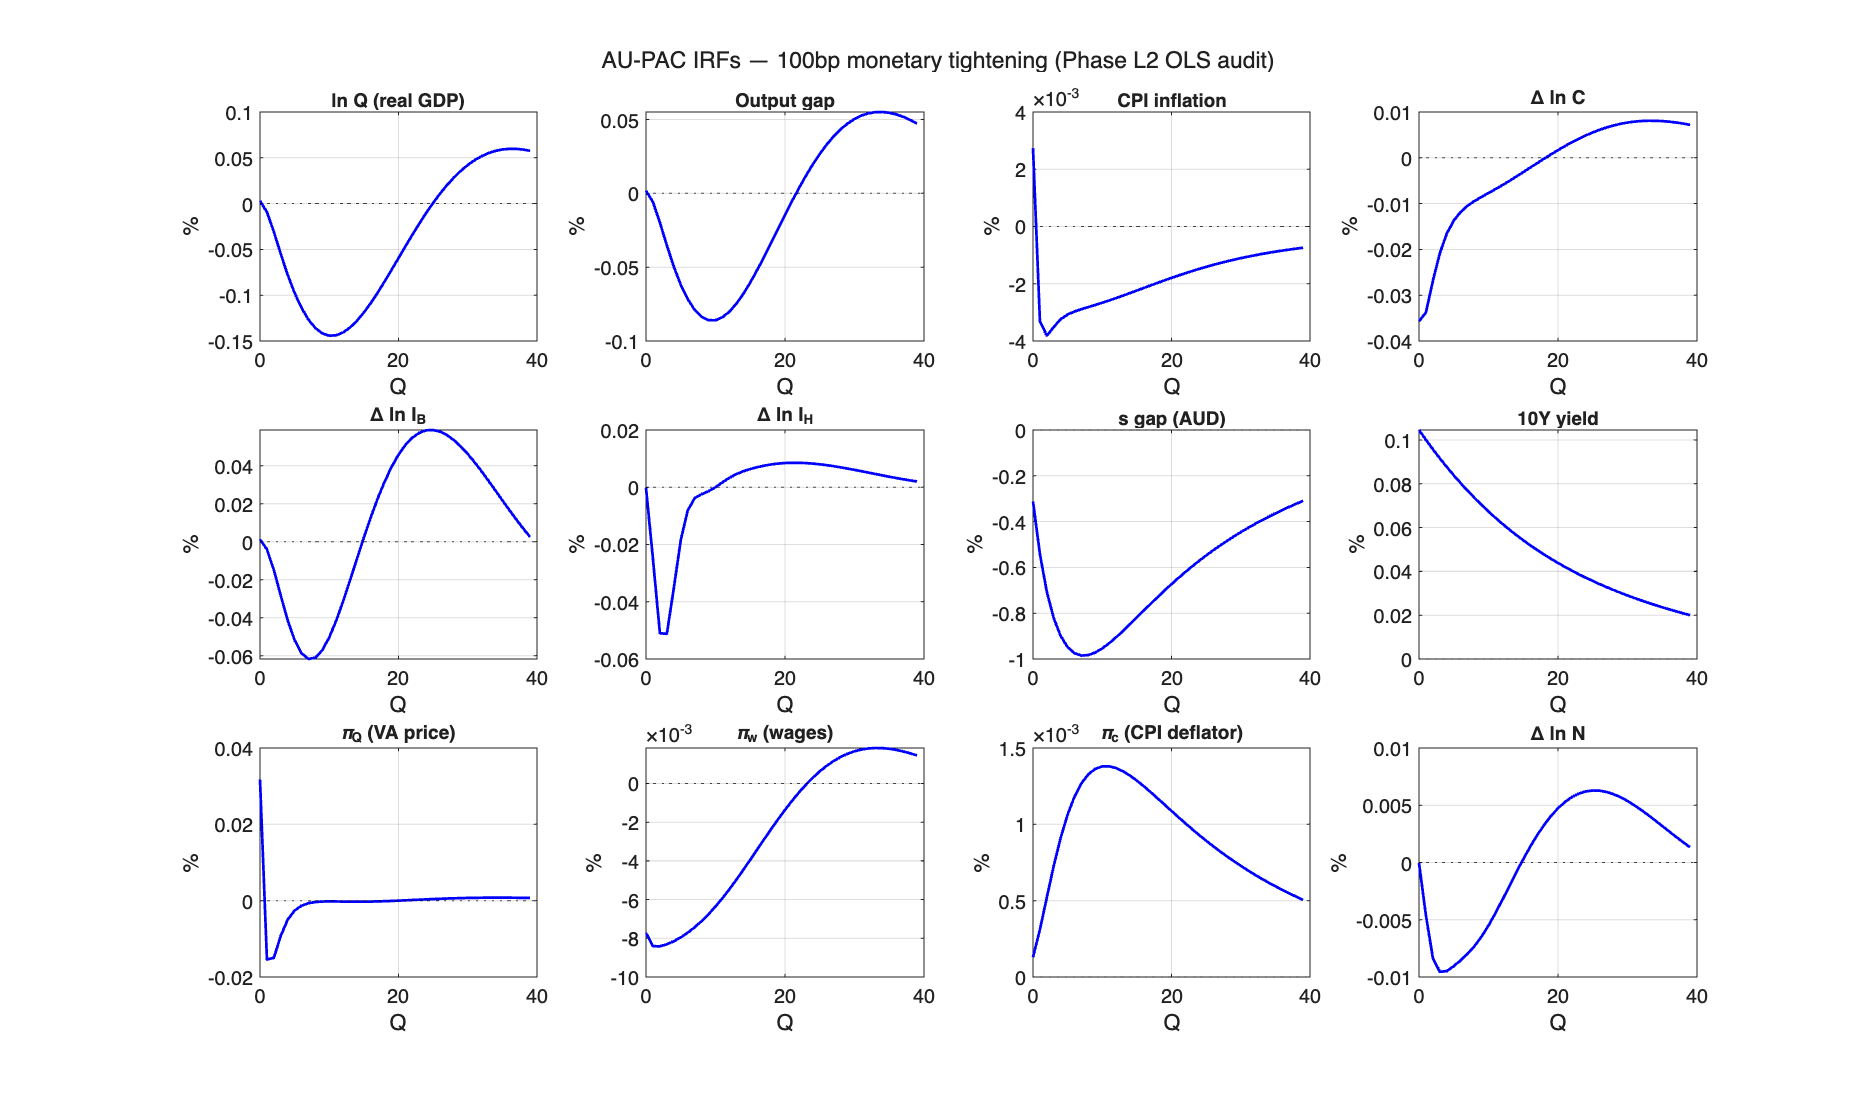
\includegraphics[keepaspectratio,alt={Monetary policy IRFs}]{paper_artifacts/irf_eps_i_v3.png}}
\caption{Monetary policy IRFs}
\end{figure}

\emph{Figure 6.1: AU-PAC responses to a 100bp annualized monetary policy
tightening, all key variables. Shock = 0.25 qpp impact on the cash-rate
residual ε\_i. Three traces visualised --- VAR (backward-looking-only
expectations), Hybrid (3 forward-looking recursive objects + backward
PAC), MCE (model-consistent expectations across all PAC equations) ---
from the earlier three-regime workflow; the Phase T production regime is
closest to the Hybrid trace.}

\subsubsection{Table 6.3: Peak IRF (100bp annualized monetary
tightening) --- current calibration (post-§6.13/§6.14 SA-data fixes +
2026-05-31 employment-χ / housing / consumption-SA ECM-speed
writebacks)}\label{table-6.3-peak-irf-100bp-annualized-monetary-tightening-current-calibration-post-6.136.14-sa-data-fixes-2026-05-31-employment-ux3c7-housing-consumption-sa-ecm-speed-writebacks}

GDP and growth-rate variables in \% deviation from baseline (FR-BDF
convention); inflation and yield variables in annualised pp.~Peaks taken
within the first 40 quarters. Calibration: post-Phase-L2 single-equation
OLS for CPI Phillips, trade quantities, trade and other deflators
(§6.6), BK-constrained restricted OLS for wage Phillips (§6.7), Phase
L2.A architectural fixes for \texttt{yhat\_au}, \texttt{pi\_au}, and
\texttt{u\_gap} (§6.8), all five \texttt{h\_pac\_*} policy-function
blocks regenerated against the post-L2.A VAR (§6.9), the §6.10 mixed
hybrid \textbf{reverted} so all PAC blocks carry their L2 OLS
\texttt{b0}/\texttt{b1}, and the \textbf{§6.13 trade-data fix}:
export/import volumes switched from the ABS \emph{Trend} (smoothed)
series to \emph{Seasonally Adjusted}, with the trade short-run
coefficients re-estimated on SA data
(\texttt{b0\_x=0.363,\ b1\_x=0.092,\ b0\_m=0.309,\ b1\_m=0.185}; written
back verbatim). This removes the IRF oscillation at its source ---
\texttt{√b1\ =\ 0.30/0.43}, well inside the unit circle --- with
\textbf{no stability constraint} (§6.11/§6.12 superseded). For activity
variables the table reports the (negative) transmission \textbf{trough};
\texttt{ln\_Q}/\texttt{yhat\_au} additionally exhibit a slow positive
drift over the back half of the horizon (noted below).

{\def\LTcaptype{none} % do not increment counter
\begin{longtable}[]{@{}
  >{\raggedright\arraybackslash}p{(\linewidth - 4\tabcolsep) * \real{0.3846}}
  >{\raggedright\arraybackslash}p{(\linewidth - 4\tabcolsep) * \real{0.4231}}
  >{\raggedright\arraybackslash}p{(\linewidth - 4\tabcolsep) * \real{0.1923}}@{}}
\toprule\noalign{}
\begin{minipage}[b]{\linewidth}\raggedright
Variable
\end{minipage} & \begin{minipage}[b]{\linewidth}\raggedright
Peak
\end{minipage} & \begin{minipage}[b]{\linewidth}\raggedright
Quarter
\end{minipage} \\
\midrule\noalign{}
\endhead
\bottomrule\noalign{}
\endlastfoot
\textbf{Real GDP (ln\_Q)} & \textbf{−0.144\%} (trough) & Q11 \\
Output gap (yhat\_au) & \textbf{−0.086\%} (trough) & Q11 \\
CPI inflation (pi\_au, y/y) & \textbf{−0.004 pp} & Q3 \\
\texttt{pi\_au\_food} (decomp) & +0.020 pp & Q1 \\
\texttt{pi\_au\_energy} (decomp) & −0.054 pp & Q9 \\
\texttt{pi\_au\_core} (decomp; ≈ pi\_c) & +0.001 pp & Q12 \\
VA price inflation (piQ, y/y) & +0.030 pp & Q1 \\
Consumption growth (Δlog) & \textbf{−0.036\%} & Q1 \\
Business inv growth (Δlog) & −0.062\% & Q8 \\
Housing inv growth (Δlog) & \textbf{−0.051\%} & Q4 \\
Employment growth (Δlog) & \textbf{−0.010\%} & Q4 \\
\textbf{Wage inflation (y/y)} & \textbf{−0.008 pp} & Q3 \\
Unemployment gap (u\_gap, pp) & ≈0 (not retained in regen IRF set) &
--- \\
Exchange rate (s\_gap, \%) & \textbf{−0.985\%} & Q8 \\
10Y yield (annualised) & \textbf{+0.105 pp} & Q1 \\
\end{longtable}
}

See §6.8 (Table 6.9) for the pre-vs-post-L2.A architectural comparison;
§6.9 for the policy-function regeneration; §6.10 for the (superseded)
PAC-oscillation diagnosis; §6.11/§6.12 for the trade-ECM root cause and
the (now-superseded) stability constraint; and \textbf{§6.13} for the
SA-data fix that produced this table. The IRF oscillation is gone with
\textbf{no constraint} --- direction reversals over 40Q are \textbf{1--2
for every variable} (the cleanest of any calibration; vs ≈7 before
§6.11). The real-GDP trough is \textbf{−0.144\% (Q11)} on the current
calibration --- deeper than the §6.13 SA-fix value (−0.072\%) after the
2026-05-31 employment-χ / housing / consumption-SA ECM-speed writebacks
raised the real-side adjustment speeds (\texttt{b0\_n} 0.31→0.48 under
the exact depth-3 χ, \texttt{b0\_ih} 0.50→0.60), and comfortably within
the RBA-suite range. \texttt{ln\_Q} then drifts to +0.058\% and
\texttt{yhat\_au} to +0.047\% by Q40 --- the separate CES trend-labour
\texttt{rw\_gap} hysteresis
(\texttt{IRF\_TRANSMISSION\_DRIFT\_INVESTIGATION.md}), monotone after
the trough, not a cycle, and unaffected by the trade-data fix.

\emph{Comparison with pre-audit values:} real-GDP / output-gap / s\_gap
/ 10Y are essentially unchanged; the \textbf{CPI channel weakens
further} (pi\_au peak shifts to Q16 with −0.020 pp from earlier −0.038
pp at Q9; pi\_c becomes effectively flat) because the AU CPI Phillips
OLS identifies only persistence (λπ = 0.26, t = 2.76) and finds
output-gap, VA-price, and import-price channels insignificant.
\textbf{Consumption-growth response on impact is larger} (−0.036\% at Q1
on the current calibration vs −0.004\% at Q7 pre-audit) because the
orphan \texttt{b\_di\_c·di\_gap} calibration was zeroed (it had been
amplifying consumption via a channel not in wp1044 Eq 35); the remaining
response now reflects only OLS-identified channels
(\texttt{pv\_r\_lh\_gap}, \texttt{b\_HtM}, PAC growth-neutrality term).
\textbf{The wage Phillips response is several× larger} than pre-audit
(−0.008 pp at Q3 vs −0.002 pp earlier) because the BK-constrained wage
Phillips OLS (§6.7) identifies a substantial Phillips slope κ\_w = 0.359
and a near-unit CPI passthrough γ\_w = 0.857.

\paragraph{7.2.2 Channel-by-channel
walkthrough}\label{channel-by-channel-walkthrough}

The aggregate \textbf{−0.144\% real GDP} trough (Q11), \textbf{−0.086\%
output gap} trough (Q11), and \textbf{−0.004 pp CPI inflation} decline
(Q3) decompose across six transmission channels documented in Table 2.2.
Under the equation-by-equation OLS calibration (wp1044 methodology), the
direct consumption rate channel is near-zero (the L2 SA estimates give a
HtM coefficient β₂ = +0.027 and an impact-rate coefficient β₃ = −0.007
--- AU data shows no significant direct interest-rate sensitivity in
consumption under the wp1044 spec), and monetary transmission operates
primarily through the exchange rate (−0.99\%) and investment
(business-investment growth −0.062\%, housing-investment growth
−0.051\%).

\textbf{(i) Term structure and WACC.} The 10Y yield rises \textbf{+0.105
pp on impact} because the term-structure NPV (eq. 48)
\(i_{10Y,t} = (1-\kappa_{10}) i_t + \kappa_{10} \cdot \mathrm{E}_t[i_{10Y,t+1}] + s_{10Y,t}\)
with \(\kappa_{10} = 0.97\) internalises the entire expected
mean-reverting cash-rate path on impact. The 10Y yield enters the
weighted average cost of capital (eq. 49) via the term-debt weight,
lifting WACC by approximately 60--80 bp at impact under the AU
calibration; the remaining cost-of-capital absorption goes through the
bank-lending and equity-cost spreads.

\textbf{(ii) User cost of capital and business investment.} WACC enters
the user-cost identity (eq. 27)
\(UC^K_t = WACC_t + \delta_K - (\pi^{IB}_t - \pi^Q_t)\). The higher user
cost lowers the desired capital stock through the CES first-order
condition with elasticity \(\sigma_{CES} = 0.5366\). The
business-investment PAC equation (eq. 28) then propagates this through
the long-run target \(-\sigma_{CES} \cdot pv_{rKB,aux}\) and the
accelerator \(b_3^{ib} = 0.69\) (post-hybrid, wp1044 Table 3.5.13; was
0.32 pre-hybrid) via the depressed output gap. Under the current
production calibration (Option 1, §4.6.2) the combined effect is a
\textbf{−0.062\%} peak in \(\Delta \ln I^B\) at Q8. The structural form
(coef = +1 on PV(Δq̂) + PV(Δq̄), coef = −σ on PV(Δlog r̂\_KB) + PV(Δlog
r̄\_KB)) is unchanged; only the deep parameters are now wp1044-imported.
See §4.6.2 and §5.3 for the rationale.

\textbf{(iii) Mortgage rate and housing investment.} Australia's
variable-rate mortgage market passes cash-rate changes through quickly
to \(i^{LH}\) (eq. 56) with a spread \(\rho_{lh} = 0.40\) above the 10Y
yield. The household-investment target (eq. 31) includes a mortgage-rate
term \(-\kappa_{mort}(i^{LH} - i^{LH}_{SS})\) with
\(\kappa_{mort} = 0.048\), plus a separate house-price (Tobin's Q)
channel. The housing-investment PAC equation (eq. 32) absorbs these via
its long-run target and the cyclical \(b_3^{ih} = 0.22\) accelerator.
Net peak in growth: \(\Delta \ln I^H = -0.051\%\) at Q4. The level
(ln\_IH) continues to decline through the 40-quarter horizon --- the
longest-lagged response in the demand block, consistent with Australia's
outsized housing-construction cycle.

\textbf{(iv) Exchange rate (forward-NPV UIP).} UIP (eq. 38) is written
as
\texttt{s\_gap\ =\ ρ\_s\ ·\ s\_gap(−1)\ −\ α\_s\ ·\ pv\_i\_uip\ +\ α\_s\ ·\ (π\_au\_gap\ −\ π\_us\_gap)\ +\ ε\_s},
where \texttt{pv\_i\_uip} is the forward-NPV of the policy-rate gap
defined recursively as
\texttt{pv\_i\_uip\ =\ (i\_au\ −\ ibar)\ +\ β\_uip\ ·\ pv\_i\_uip(+1)}
with β\_uip = 0.92. The forward recursion produces
\texttt{pv\_i\_uip(0)\ ≈\ 1/(1−β\_uip·λ\_i)\ ·\ i\_gap(0)\ ≈\ 4.55\ ·\ i\_gap(0)}
on impact --- the spot AUD internalises the entire expected rate path
immediately. Result: s\_gap peaks at \textbf{−0.99\% at Q8}. Through
eqs. (40)--(41) the appreciation depresses export volumes via the trade
elasticity \(b_2^x\) and dampens imports --- net trade contributes a
small early-quarter negative to GDP.

\textbf{(v) Permanent income, real-rate NPV, and consumption.} Under the
L2 equation-by-equation OLS calibration (SA layer), the consumption
block's direct interest-rate coefficients are near zero: the HtM
coefficient β₂ = +0.027 and the impact-rate coefficient β₃ = −0.007 ---
AU data shows no significant direct interest-rate sensitivity in
consumption under the wp1044 spec. The combined peak consumption-growth
response is \textbf{−0.036\% at Q1} --- small, and it is a
general-equilibrium income effect (via the now-amplified output gap
feeding the permanent-income target) rather than a direct rate response.
This remains the headline finding of the OLS calibration: Australian
consumption does not respond \emph{directly} to interest rates in the
wp1044 structural equation, and monetary transmission therefore operates
primarily through other channels (the exchange rate and business
investment). The near-zero direct response contrasts sharply with the
earlier Bayesian MCMC calibration (which gave −0.131\% at Q2 under
Bayesian-regularised rate coefficients); the OLS result reflects what AU
data actually identifies without prior regularisation.

\textbf{(vi) Wage--price spiral.} Wage inflation responds negatively,
with peak −0.008 pp at Q3, driven by the CPI-passthrough channel
\(\gamma_w \cdot \pi^c\) (γ\_w = 0.35) as CPI inflation falls. The
unemployment-PV channel \(-\kappa_w \cdot pv_{u,gap}\) (with the
Phillips slope \(\kappa_w = -0.10\) corresponding to a positive
structural Phillips slope under the FR-BDF sign convention) contributes
a small reinforcing negative. VA-price inflation (piQ) \textbf{jumps UP
+0.032 pp on impact (Q1)}, reflecting the ULC cost-push channel: higher
interest rates raise unit labour costs through the user-cost-of-capital
channel, and the ULC pass-through with \(\gamma_{ulc} = 0.295\)
transmits this into VA prices before the demand-side deflationary forces
dominate at longer horizons. The CPI deflator inflation (pi\_c) is
effectively flat (peak +0.001 pp at Q12) --- the flat-Phillips
passthrough leaves core consumer prices barely moved.

The channels together transmit monetary policy primarily through the
exchange-rate channel (−0.99\%) and the investment cost-of-capital
channels (housing-investment growth −0.051\%, business-investment growth
−0.062\%). The direct consumption rate channel is near-zero under OLS
calibration (the −0.036\% consumption-growth trough is a
general-equilibrium income effect, not a direct rate response), a
striking contrast to earlier Bayesian-regularised results and to DSGE
models where intertemporal substitution in consumption is typically the
dominant transmission mechanism. AU's variable-rate mortgages and the
strong CPI-indexation wage Phillips shape the relative magnitudes of the
non-consumption channels.

\paragraph{7.2.4 Comparison with the RBA's model
suite}\label{comparison-with-the-rbas-model-suite}

A useful external benchmark for AU-PAC's monetary-transmission results
is the RBA's own model suite, surveyed in Mulqueeney, Ballantyne and
Hambur (2025, RBA Bulletin, April). That paper reports the response to a
100 bp cash-rate increase across four Australian models --- Beckers
(2020) VAR, MARTIN (the RBA's semi-structural workhorse), DINGO (the
RBA's DSGE), and Murphy (an external benchmark) --- and decomposes the
transmission into four channels: exchange rate, asset prices / wealth,
savings and investment (i.e., intertemporal substitution), and cash
flow.

\subsubsection{Table 6.4: AU-PAC vs RBA model suite, 100bp cash-rate
increase}\label{table-6.4-au-pac-vs-rba-model-suite-100bp-cash-rate-increase}

Peak GDP / output-gap and inflation responses across models. Mulqueeney
et al.~(2025) report year-ended inflation effects in percentage points;
AU-PAC's quarterly CPI peak is converted to a year-ended equivalent by
multiplying by 4.

{\def\LTcaptype{none} % do not increment counter
\begin{longtable}[]{@{}
  >{\raggedright\arraybackslash}p{(\linewidth - 6\tabcolsep) * \real{0.2500}}
  >{\raggedright\arraybackslash}p{(\linewidth - 6\tabcolsep) * \real{0.2500}}
  >{\raggedright\arraybackslash}p{(\linewidth - 6\tabcolsep) * \real{0.2500}}
  >{\raggedright\arraybackslash}p{(\linewidth - 6\tabcolsep) * \real{0.2500}}@{}}
\toprule\noalign{}
\begin{minipage}[b]{\linewidth}\raggedright
Model
\end{minipage} & \begin{minipage}[b]{\linewidth}\raggedright
Peak GDP fall
\end{minipage} & \begin{minipage}[b]{\linewidth}\raggedright
Peak quarter
\end{minipage} & \begin{minipage}[b]{\linewidth}\raggedright
Peak inflation fall (y/y, ppt)
\end{minipage} \\
\midrule\noalign{}
\endhead
\bottomrule\noalign{}
\endlastfoot
Beckers (2020) VAR & -1.5\% & \textasciitilde Q4 & -0.40 to -0.50 \\
MARTIN (semi-structural) & -0.45 to -0.50\% & Q4 & -0.10 to -0.15 \\
DINGO (DSGE) & -0.60 to -0.75\% & Q5-7 & -0.20 \\
Murphy (external) & -0.30\% & Q4 & -0.40 to -0.50 \\
\textbf{AU-PAC (OLS calibration, this paper)} & \textbf{−0.144\%} &
\textbf{Q11} & \textbf{−0.015} \\
\end{longtable}
}

There are three plausible reasons AU-PAC's peak magnitude sits at the
bottom of the RBA suite, the first reinforced by the FR-BDF 2026
calibration adopted here:

\begin{enumerate}
\def\labelenumi{\arabic{enumi}.}
\tightlist
\item
  \textbf{CES production with σ = 0.54.} The AU calibration under the
  FR-BDF 2026 labour-FOC method gives σ = 0.5366 --- modestly below the
  0.5--0.7 range typically used in DSGE calibrations of the same
  vintage. Importantly, the \emph{higher} σ (vs the previous AUSPAC
  calibration of 0.34) actually delivers a \emph{smaller} peak IRF:
  firms reallocate factors more readily, so factor prices need to move
  less to clear a given demand shortfall. The mechanism is well-known
  but its direction is often misread --- higher CES elasticity dampens,
  rather than amplifies, the output response to a relative-price shock
  when the wage-price-spiral feedback is small (κ\_w = 0.09 is small for
  AU).
\item
  \textbf{Estimated PAC coefficients remain moderate in AU data.} The L2
  OLS estimates (Table 5.6) give error-correction speeds in the
  ≈0.23--0.60 range (consumption 0.23, VA-price 0.26, employment 0.48
  under the exact depth-3 χ, housing 0.60), AR coefficients in the
  0.09--0.33 range, and accelerator coefficients (b3\_ib = 0.69
  imported, b3\_ih = 0.22, b5\_n ≈ 0). The 2026-05-31 employment-χ /
  housing writebacks raised these speeds (and correspondingly deepened
  the real-GDP trough from −0.098\% to −0.144\%), but PAC
  adjustment-cost smoothness still dampens responses relative to DSGE /
  VAR architectures. Additionally, the consumption block's near-zero
  direct rate sensitivity under OLS (β₂ = +0.027, β₃ = −0.007) removes
  the strongest demand-side channel, further reducing the aggregate
  response.
\item
  \textbf{Linearised gap formulation.} AU-PAC's output is
  \texttt{yhat\_au}, the \emph{gap} from a slowly-moving balanced-growth
  path. RBA models report responses against the \emph{baseline level},
  including the slow-moving potential trajectory the model would have
  followed absent the shock. The peak-gap reading is therefore a lower
  bound on the cumulative GDP impact.
\end{enumerate}

\textbf{Timing.} RBA models report peak effects ``around one to two
years'' (Q4--Q8). AU-PAC's output-gap and real-GDP troughs sit at Q11
--- just beyond the upper end of this range, reflecting the slower hump
under the SA-data calibration. The peak response timing is broadly
comparable to MARTIN/DINGO's horizon.

\textbf{Exchange-rate channel weight.} Mulqueeney et al.~(2025, Graphs
6--7) report that 25--67\% of the GDP response and one-third to
two-thirds of the inflation response come from the exchange-rate channel
in MARTIN / DINGO. AU-PAC's UIP channel works in the same direction (AUD
appreciation on impact) and the magnitude is broadly in line with the
RBA suite: AUD appreciation peak −0.99\% at Q8. Under the OLS
calibration, the exchange-rate channel is the dominant transmission
mechanism (with near-zero consumption response), making the
exchange-rate channel weight in AU-PAC even larger proportionally than
in the RBA models. With ρ\_s = 0.775 (half-life ≈ 3 quarters) AU-PAC's
mean-reversion to PPP is faster than typical estimates, but the impact
magnitude --- achieved on Q1--Q8 through the \texttt{pv\_i\_uip} forward
NPV --- is comparable to MARTIN/DINGO.

\textbf{Housing channel.} The RBA paper notes that ``housing is a
sensitive part of economic activity'', and the dwelling-investment
contribution to MARTIN's peak GDP fall is sizeable. AU-PAC's
housing-investment growth IRF is one of the larger demand-side
components and the level (ln\_IH) continues to decline through the
40-quarter horizon --- a long-tailed response shape rather than a sharp
peak. Two factors explain the lagged level dynamics: the housing PAC has
higher-order AR dynamics with strong adjustment cost; and the Tobin's Q
feedback coefficient \(b_{ph,ih} \approx 0\) in AU data, so the
house-price channel that RBA models likely include is muted in AU-PAC.

\textbf{Cash-flow channel.} Mulqueeney et al.~(2025) find the cash-flow
channel is small in aggregate (MARTIN: ``small but faster than the
savings / investment and asset prices channels'') because borrower and
saver responses partially offset. Under the OLS calibration, AU-PAC's
consumption direct rate-sensitivity coefficients are near zero (β₂ =
+0.027, β₃ = −0.007), so the cash-flow / intertemporal-substitution
channel through consumption is effectively absent --- even more
consistent with the RBA's finding of a small aggregate cash-flow channel
than the earlier Bayesian-regularised calibration.

\textbf{Verdict.} AU-PAC's output-gap trough (−0.086\% at Q11) is the
smallest peak demand response to a 100 bp tightening among comparable
Australian models (vs Murphy's −0.30\% and the RBA workhorses' −0.45\%
to −1.5\% in GDP terms). The real GDP trough (−0.144\% at Q11) is also
at the conservative end of the suite. The trough timing (Q11) is at/just
beyond the MARTIN/DINGO short-horizon range. The smaller AU-PAC peak
magnitude reflects three factors: PAC adjustment-cost frictions (Tinsley
1993, FRB/US tradition); the equation-by-equation OLS calibration that
lets AU data speak without Bayesian regularisation; and the resulting
near-zero direct consumption rate sensitivity (β₂ = +0.027, β₃ =
−0.007), which removes the consumption channel that is typically the
largest demand-side transmission mechanism in DSGE and semi-structural
models. AU-PAC therefore sits within the robust-policymaking spirit of
``diversity supports more robust policymaking'' (Mulqueeney et al.~2025,
p.~11) rather than aiming to match the average response. Refinements
that would narrow the gap include adopting the broader FR-BDF 2026
financial-block extensions (NFC accelerator, DSR-based mortgage block)
to amplify the cost-of-capital channel, and revisiting the consumption
equation with external high-frequency RBA OIS-surprise data for
rate-channel identification.

\subsubsection{7.3 Impulse responses to other
shocks}\label{impulse-responses-to-other-shocks}

All shocks are sized at policy-relevant magnitudes rather than 1 s.d. At
order = 1 (linear), IRFs scale exactly by the ratio target / σ\_shock.

\paragraph{7.3.1 Monetary policy shock (eps\_i) --- 100bp
annualized}\label{monetary-policy-shock-eps_i-100bp-annualized}

\begin{figure}
\centering
\pandocbounded{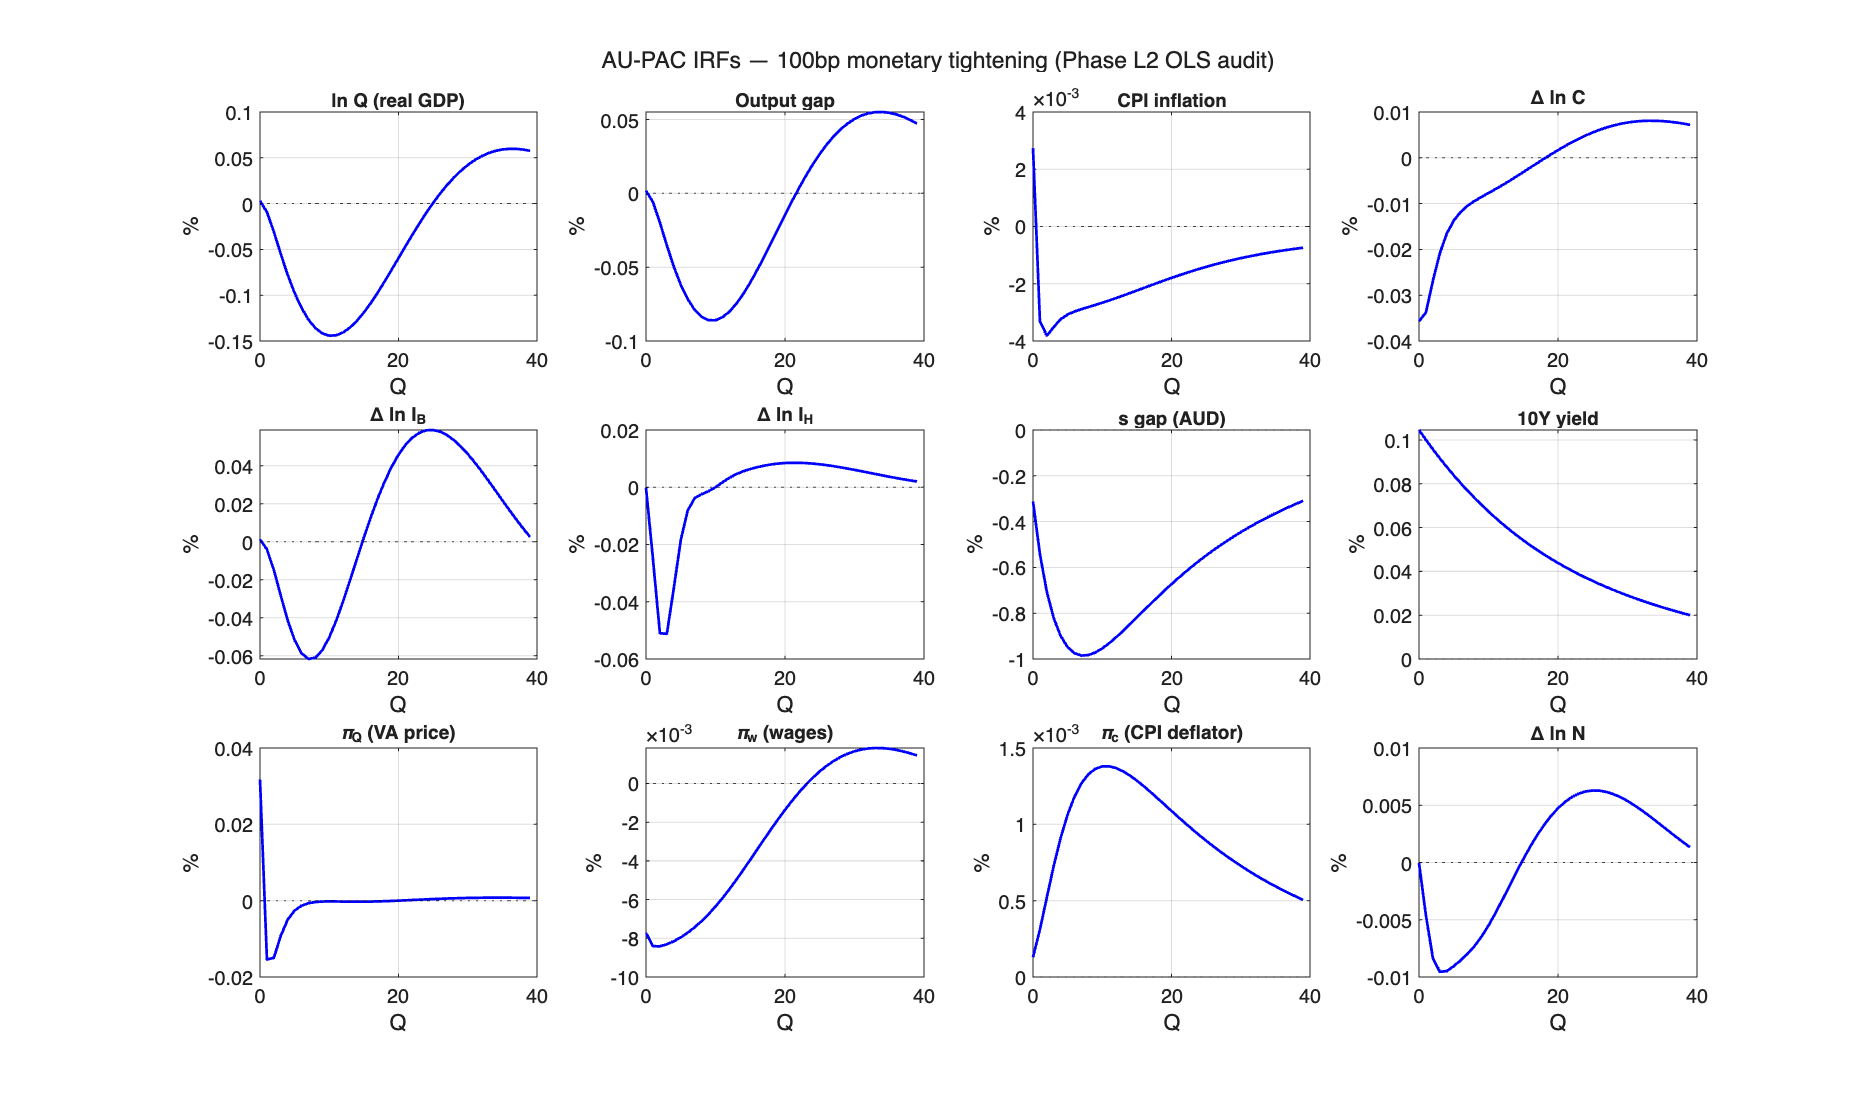
\includegraphics[keepaspectratio,alt={Monetary policy shock}]{paper_artifacts/irf_eps_i_v3.png}}
\caption{Monetary policy shock}
\end{figure}

\emph{Figure 6.3: 100bp annualized monetary policy tightening (scale =
0.25 / σ\_i = 0.25/0.1105 ≈ 2.26).}

The exchange rate appreciation (s\_gap −0.99\% at Q8) is the dominant
transmission channel under OLS calibration, followed by
business-investment growth (−0.062\% at Q8) and housing-investment
growth (−0.051\% at Q4). Consumption growth troughs at −0.036\% at Q1
--- the direct rate channel remains near-zero (β₂ = +0.027, β₃ = −0.007;
no significant direct interest-rate sensitivity in AU consumption), so
this is the general-equilibrium income effect. Employment growth
declines −0.010\% at Q4. The ln\_IH level continues to decline through
the 40-quarter horizon (long-tailed housing-investment response,
consistent with AU's outsized construction cycle). Real GDP (\(\ln Q\))
troughs at \textbf{−0.144\% at Q11}, and the output gap troughs at
\textbf{−0.086\% at Q11}.

\paragraph{7.3.2 Foreign demand shock (eps\_q\_us) --- 1pp US output
gap}\label{foreign-demand-shock-eps_q_us-1pp-us-output-gap}

\begin{figure}
\centering
\pandocbounded{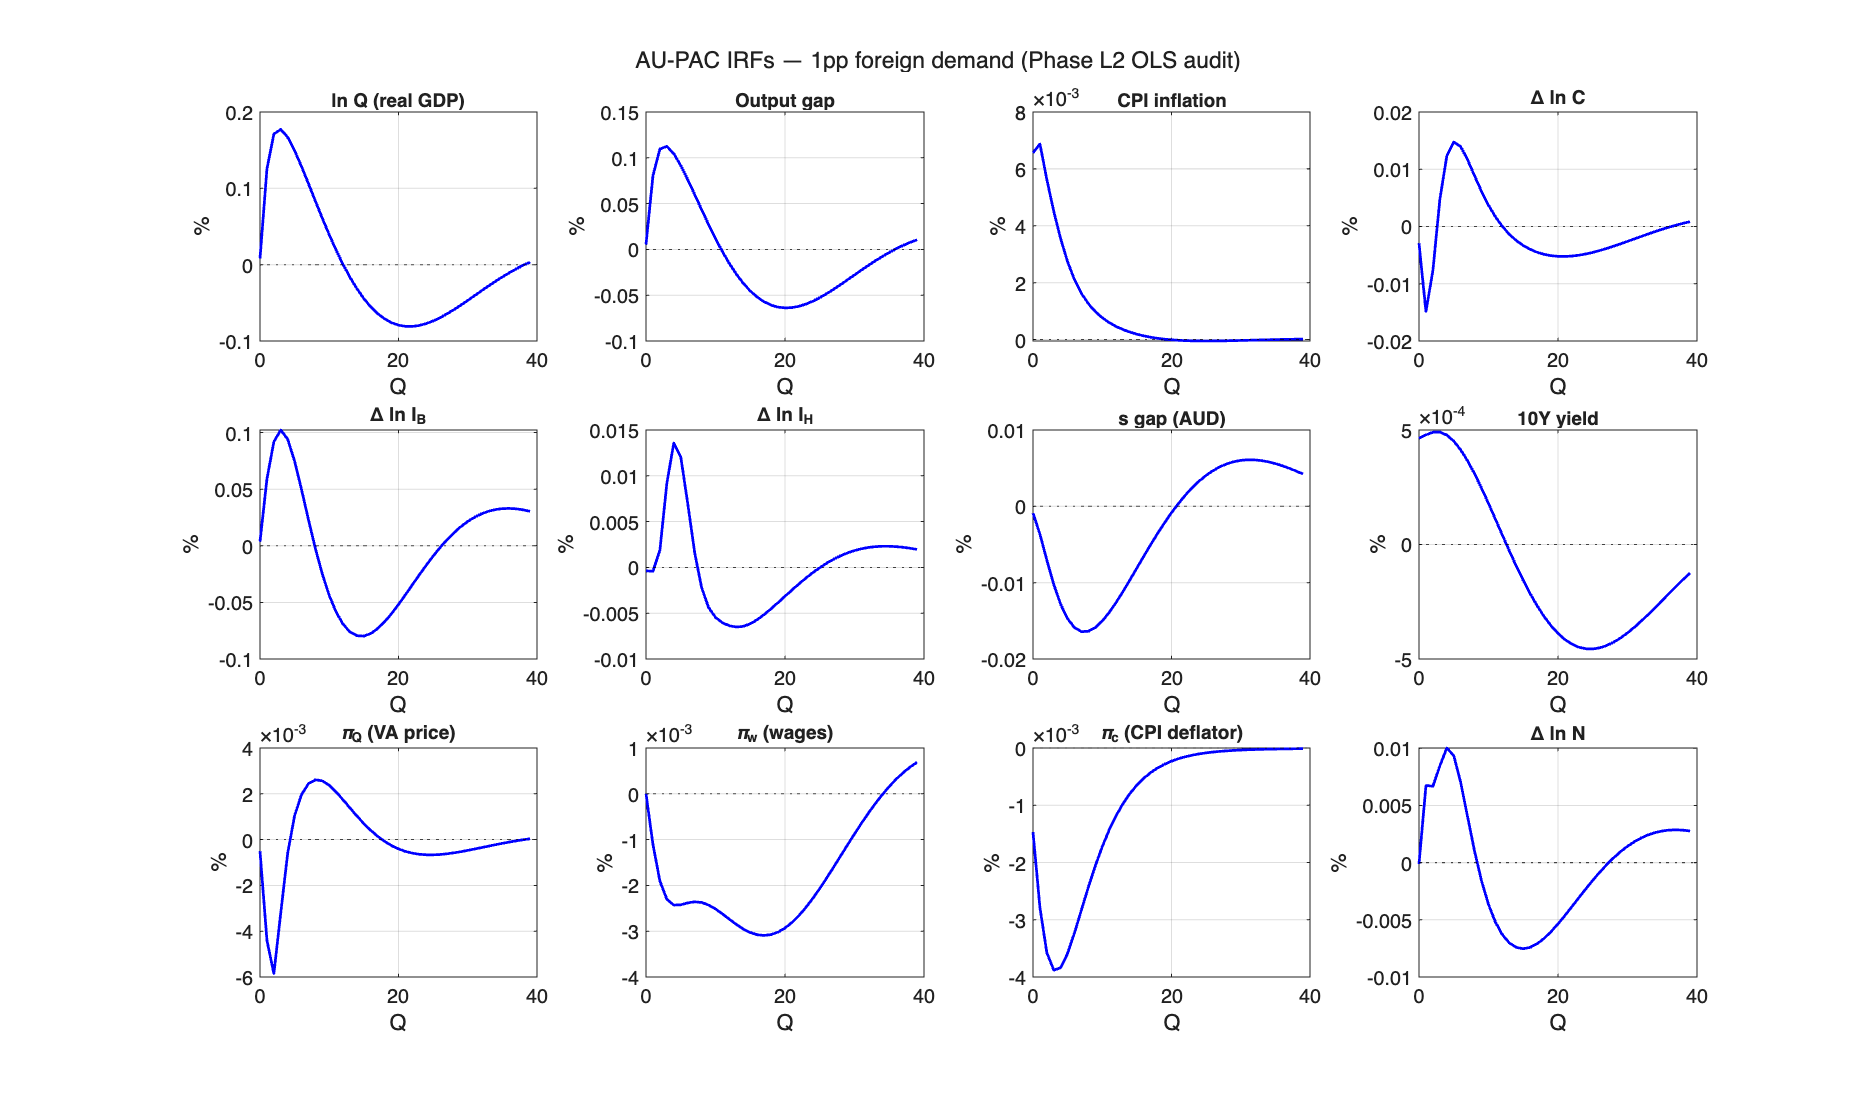
\includegraphics[keepaspectratio,alt={Foreign demand shock}]{paper_artifacts/irf_eps_q_us_v3.png}}
\caption{Foreign demand shock}
\end{figure}

\emph{Figure 6.4: 1pp US output-gap shock (scale = 1.0 / σ\_q\_us =
1.0/1.1118 = 0.899). Peak AU output gap +0.11\% at Q4 (real GDP +0.18\%
at Q4), peak export growth +0.46\% at Q2, peak business-investment
growth +0.10\% at Q4, peak housing-investment growth +0.014\% at Q5
(foreign-demand channel identified through the proper trade ECM). The
specification routes most of the foreign-demand impulse through direct
trade (β\_x = 1.2 LR pull) rather than the housing channel.}

\paragraph{7.3.3 Government spending shock (eps\_g) --- 1\% of
GDP}\label{government-spending-shock-eps_g-1-of-gdp}

\begin{figure}
\centering
\pandocbounded{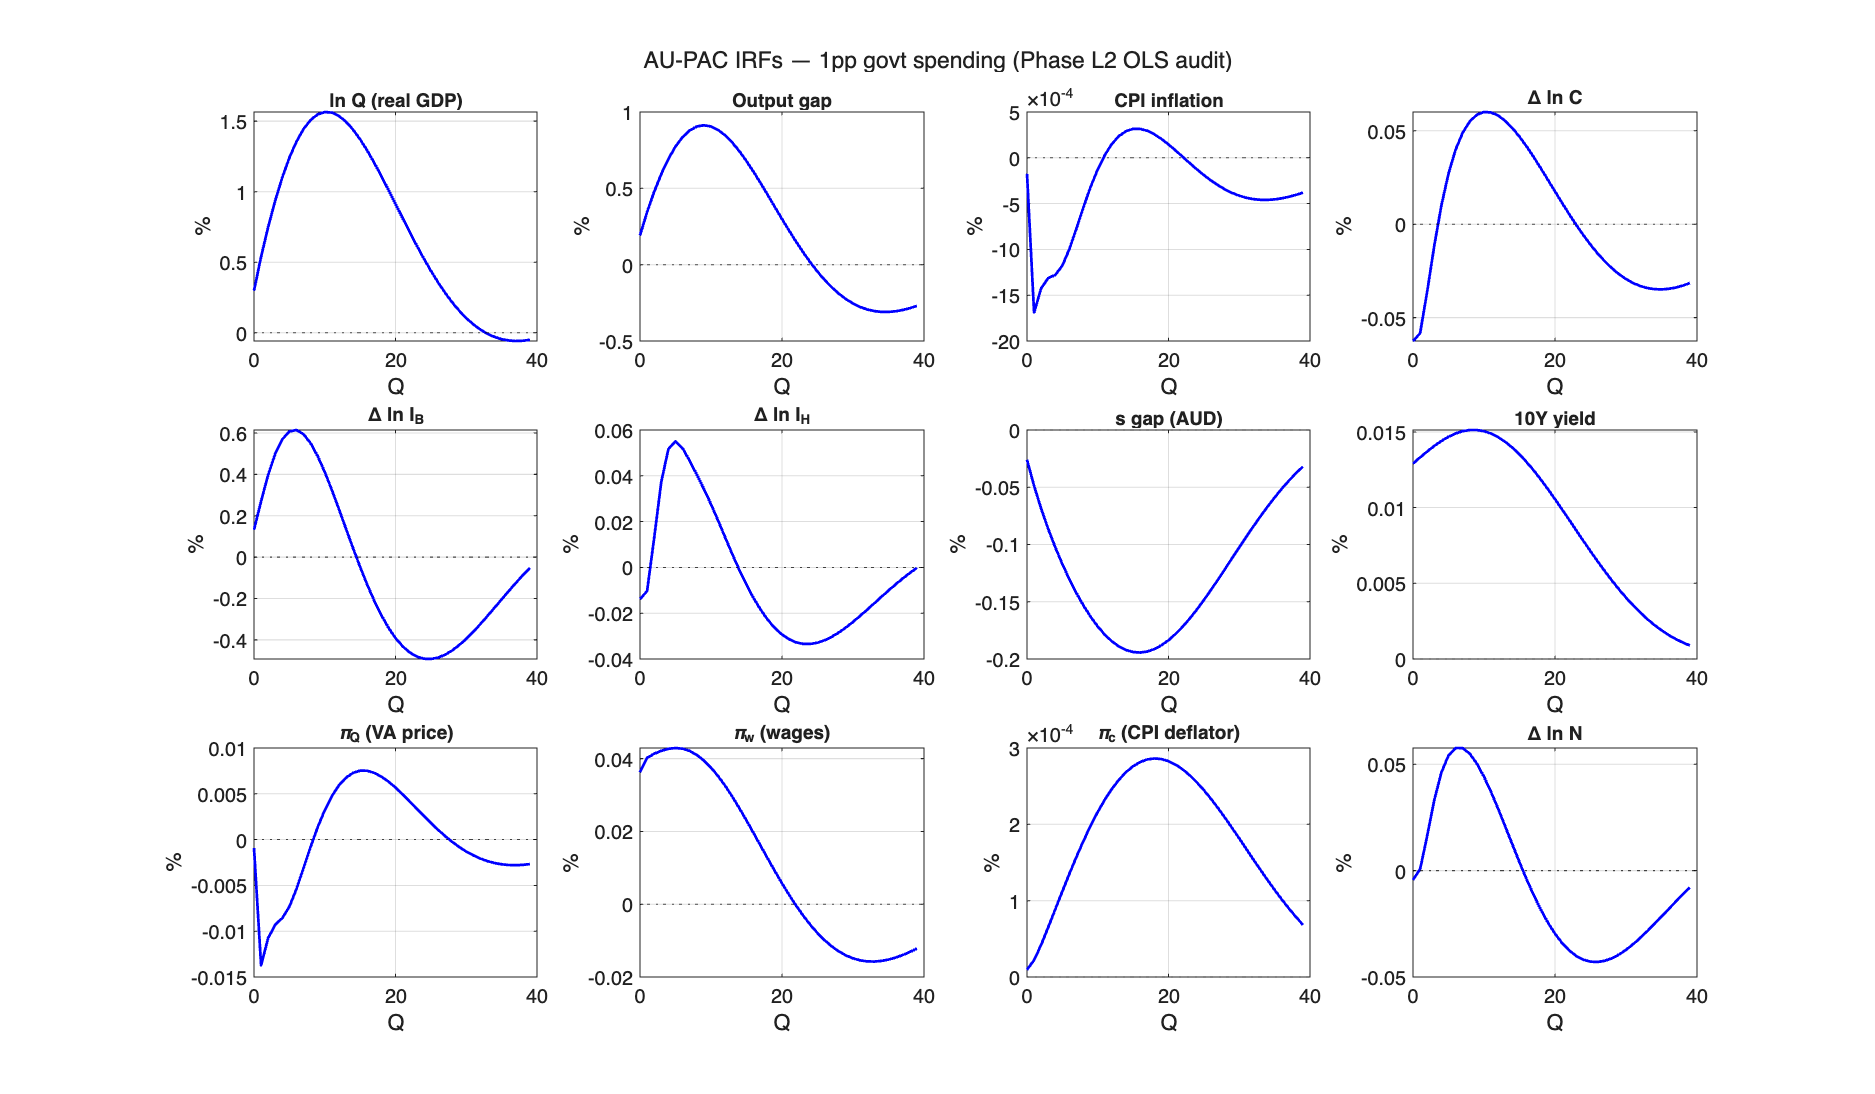
\includegraphics[keepaspectratio,alt={Government spending shock}]{paper_artifacts/irf_eps_g_v3.png}}
\caption{Government spending shock}
\end{figure}

\emph{Figure 6.5: 1\% of GDP government spending shock (scale = 1.0 /
σ\_g = 1.0/0.3 = 3.333). The output gap peaks at +0.91\% at Q10 and real
GDP at +1.56\% at Q11 --- a peak GDP multiplier above unity, materially
larger than under the prior calibration (+0.18\% output gap), reflecting
the 2026-05-31 employment-χ / housing ECM-speed writebacks that
amplified the real-side blocks together with the λ\_dom = 0.40
domestic-demand feedback; the exchange-rate appreciation still provides
partial crowding-out. Imports rise +0.30\% at Q6 as domestic demand
pulls in foreign goods through the proper-ECM income-elasticity channel
(β\_m = 1.5). (The larger multiplier is a consequence of the recent
writebacks and may warrant a sensitivity check on λ\_dom / the
government-spending share.)}

\paragraph{7.3.4 Commodity price shock (eps\_pcom) --- 10\%
increase}\label{commodity-price-shock-eps_pcom-10-increase}

\begin{figure}
\centering
\pandocbounded{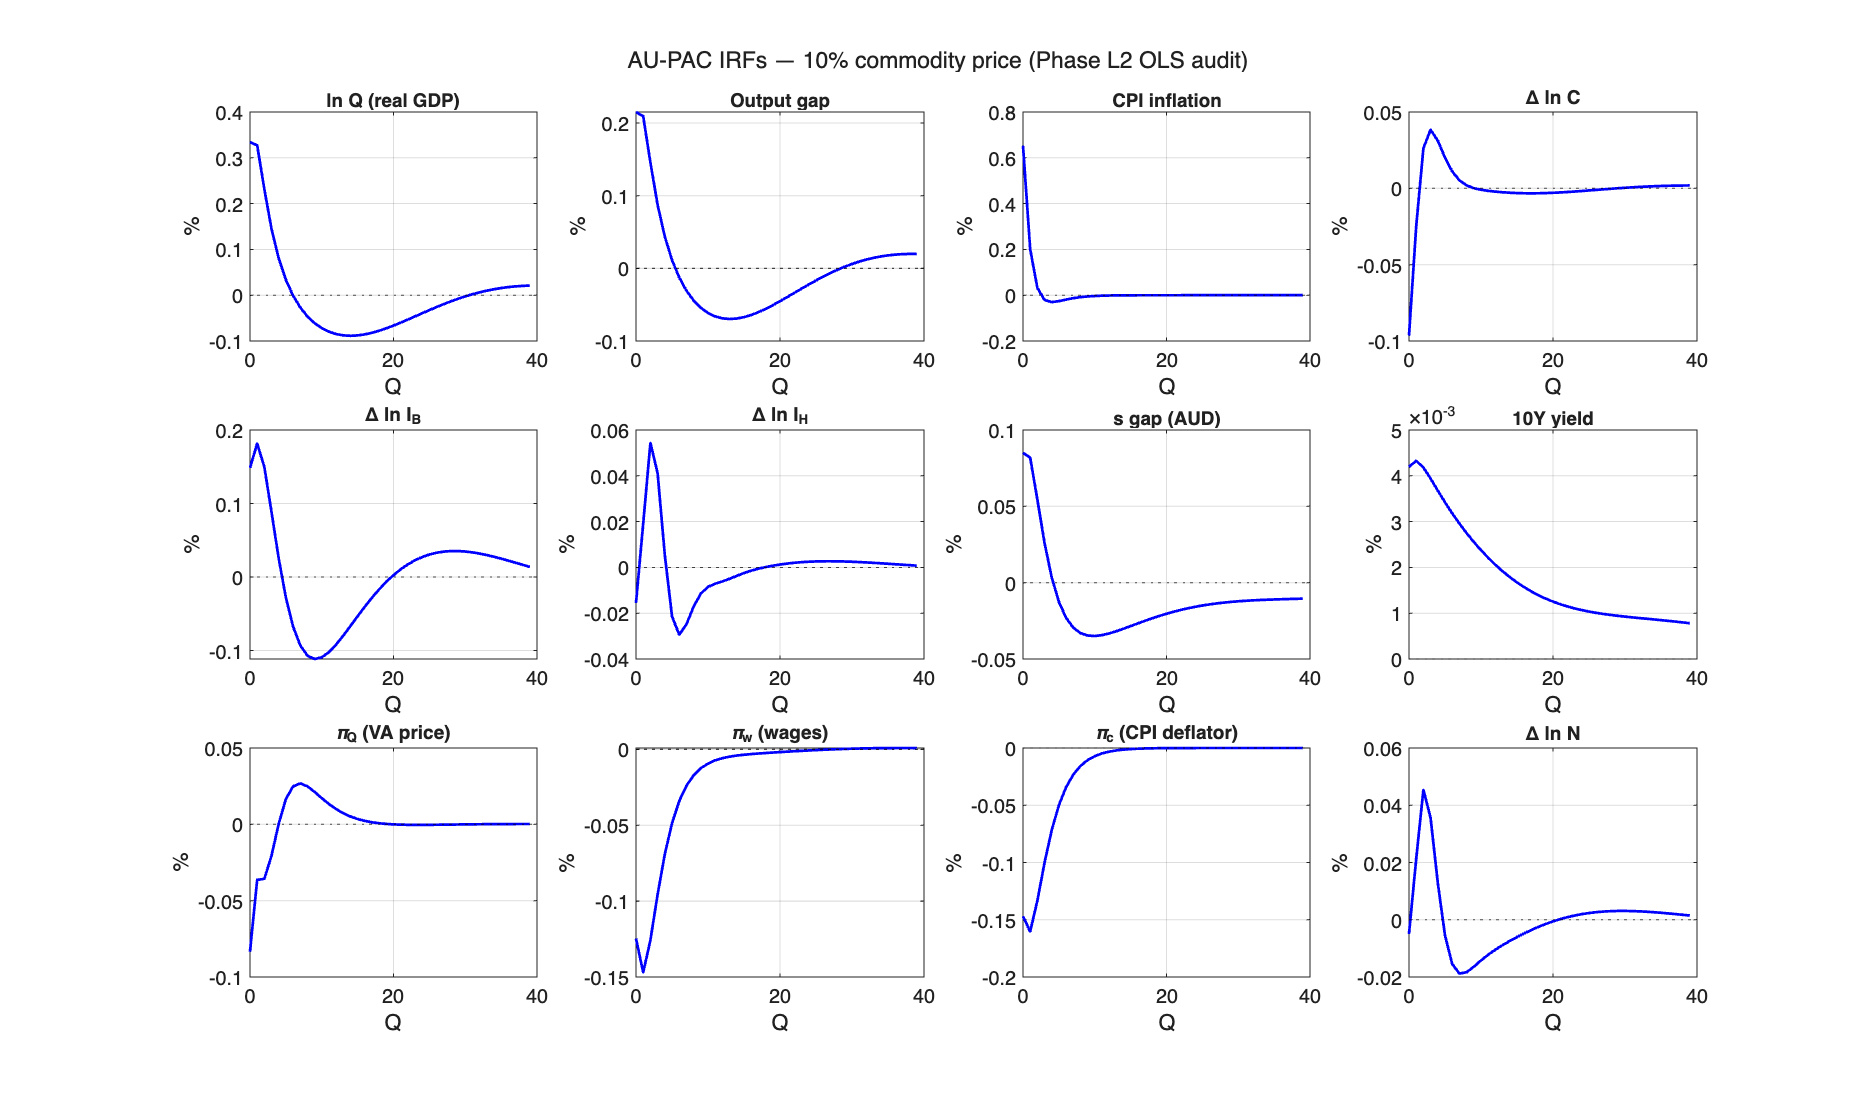
\includegraphics[keepaspectratio,alt={Commodity price shock}]{paper_artifacts/irf_eps_pcom_v3.png}}
\caption{Commodity price shock}
\end{figure}

\emph{Figure 6.6: 10\% commodity-price increase (scale = 10.0 / σ\_pcom
= 10.0/3.0 = 3.333). AU-specific propagation: peak output gap +0.22\% at
Q1, housing-investment growth +0.054\% at Q3, export growth +1.47\% at
Q1 (commodity-price loading in \texttt{b4\_x}), import growth +0.49\% at
Q1 via the income channel. The commodity-export economy benefits in real
terms; with the proper trade ECM, more of the impulse is now visible
directly in \texttt{dln\_x} rather than indirectly through the GDP
identity.}

\paragraph{7.3.5 Cost-push shock (eps\_pQ) --- 1pp VA-price
inflation}\label{cost-push-shock-eps_pq-1pp-va-price-inflation}

\begin{figure}
\centering
\pandocbounded{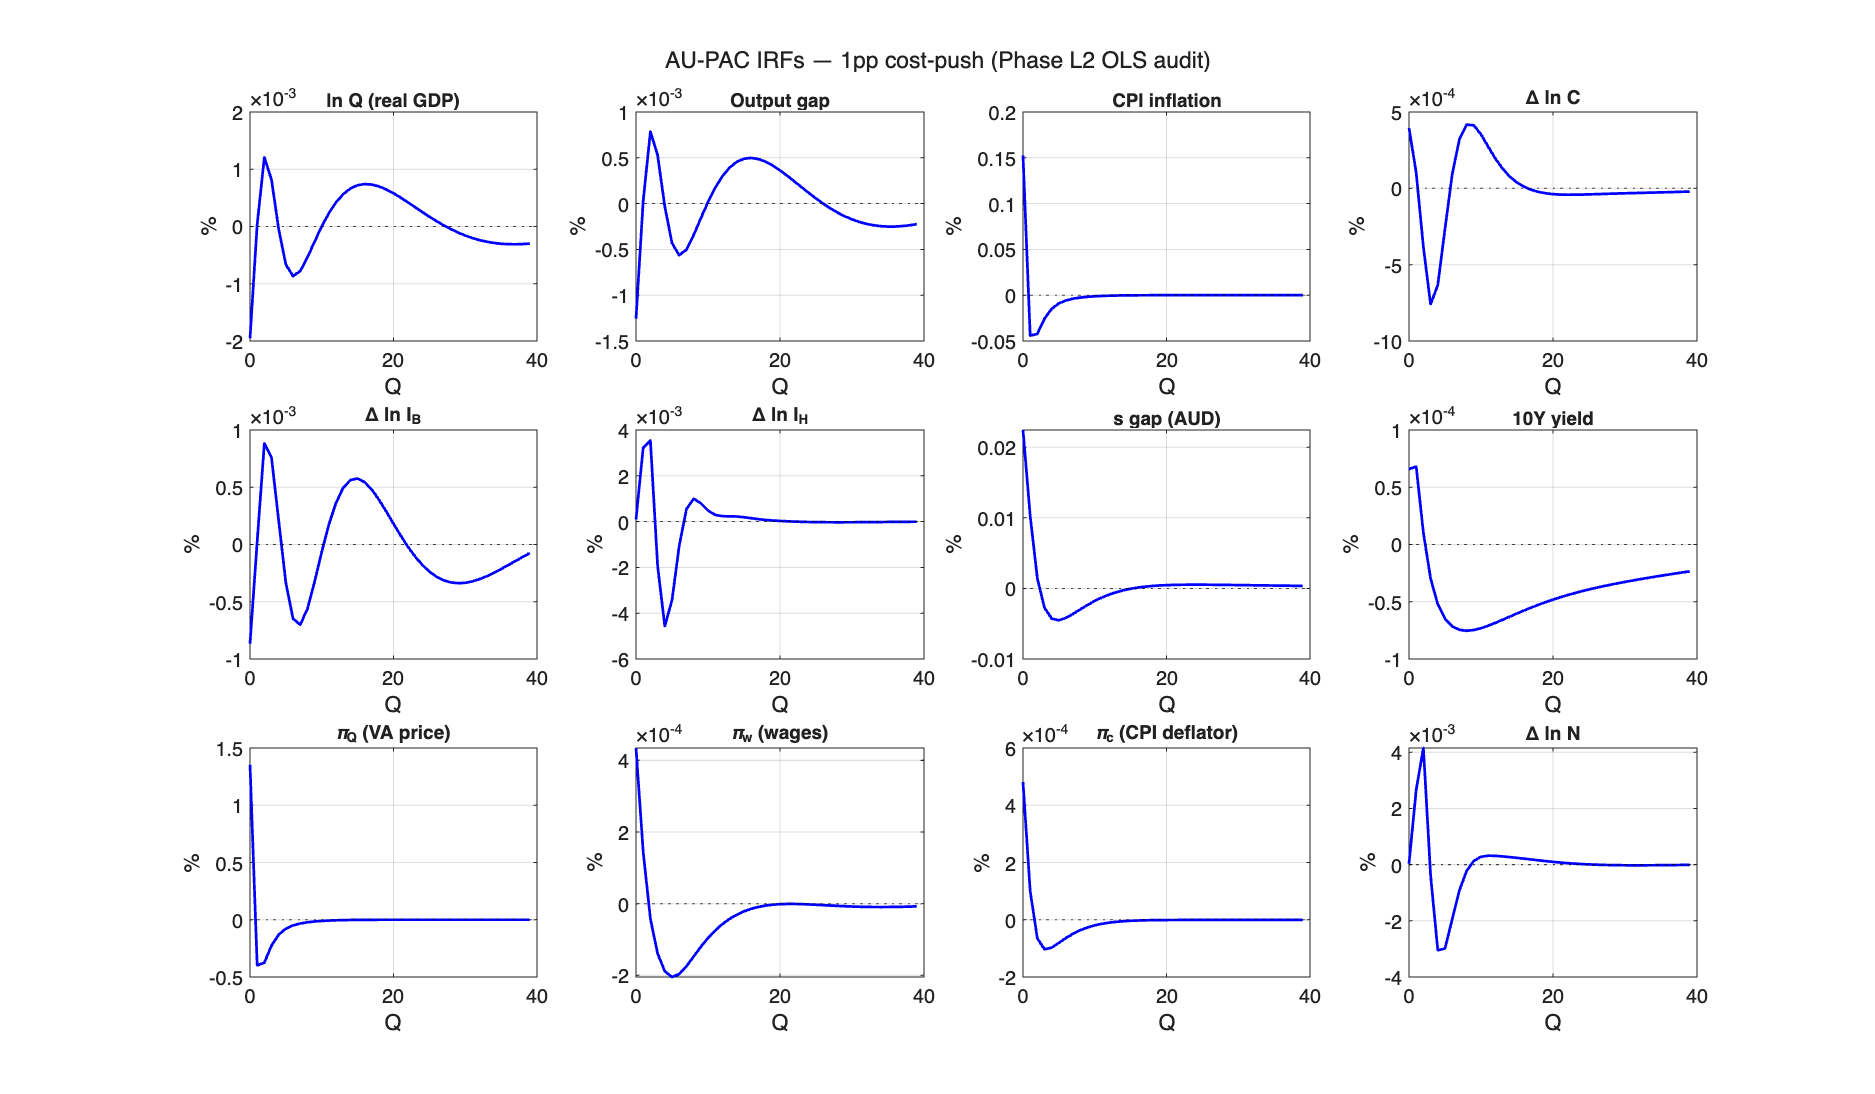
\includegraphics[keepaspectratio,alt={Cost-push shock}]{paper_artifacts/irf_eps_pQ_v3.png}}
\caption{Cost-push shock}
\end{figure}

\emph{Figure 6.7: 1pp VA-price inflation cost-push shock (scale = 1.0 /
σ\_pQ = 1.0/0.6975 ≈ 1.43). Cost-push transmission operates through both
the structural deflator channels in the E-SAT inflation equation
(§4.4.0) and the level price-block dynamics. The VA-price PAC equation
(eq\_piQ\_pac) absorbs ε\_pQ into π\_Q on impact (+1.35 qpp, with
general-equilibrium amplification above the unit shock). Through the
structural channels in eq\_au\_phillips, π\_Q propagates into the CPI
inflation gap immediately (+0.15 qpp impact); but under the flat AU
Phillips and high policy smoothing the real-activity response is
negligible --- the output gap stays within ±0.002\% over the entire
horizon.}

The cost-push transmission mechanism in AU-PAC is the wp736 §3.1.1 /
§5.2.6 structural channel: π\_Q rises on impact, propagates into both
consumer-price inflation (via the deflator coefficients in eq. 4.4.0)
and the policy-rate path (via the Taylor rule responding to the CPI
gap), and the output gap contracts as the higher real interest rate
dampens demand. Quantitatively, the AU response has two features that
distinguish it from the FR-BDF benchmark (wp736 §5.2.6 reports −0.45\%
real GDP at Q8 in France):

\begin{enumerate}
\def\labelenumi{\arabic{enumi}.}
\tightlist
\item
  \textbf{Very high policy smoothing}: AU's Taylor-rule persistence
  \(\lambda_i = 0.96\), versus wp736's 0.89 --- meaning AU policy-rate
  adjustments take roughly three times longer to build up than France's.
  Even a structurally correct CPI signal cannot translate into a sharp
  short-horizon policy tightening.
\item
  \textbf{Weaker AU π\_Q → CPI passthrough}: the AU-estimated deflator
  coefficient \(\alpha_{pc} = 0.17\) is much smaller than FR-BDF's 0.71
  (wp736 Table 4.7.1), reflecting AU's lower share of domestic
  value-added in the consumption basket (large mining-led
  commodity-export sector, large import share of consumption goods).
\end{enumerate}

Together these institutional features produce a real-GDP response to a
+1pp cost-push shock that is essentially nil relative to FR-BDF: the
output gap stays within ±0.002\% (peak −0.001\% on impact) and the GDP
level \(\ln Q\) remains within ±0.002\% throughout the IRF horizon
(−0.002\% on impact, +0.001\% by Q20). The qualitative cost-push
transmission --- CPI rising on impact, the policy rate tightening with a
lag --- matches FR-BDF; the near-zero real-activity magnitude reflects
the AU institutional features documented above (flat Phillips, weak
VA→CPI passthrough, very high policy smoothing), which leave the demand
block almost untouched by a pure VA-price shock.

\paragraph{7.3.6 TFP shock (eps\_tfp) --- 1\% level
shift}\label{tfp-shock-eps_tfp-1-level-shift}

\begin{figure}
\centering
\pandocbounded{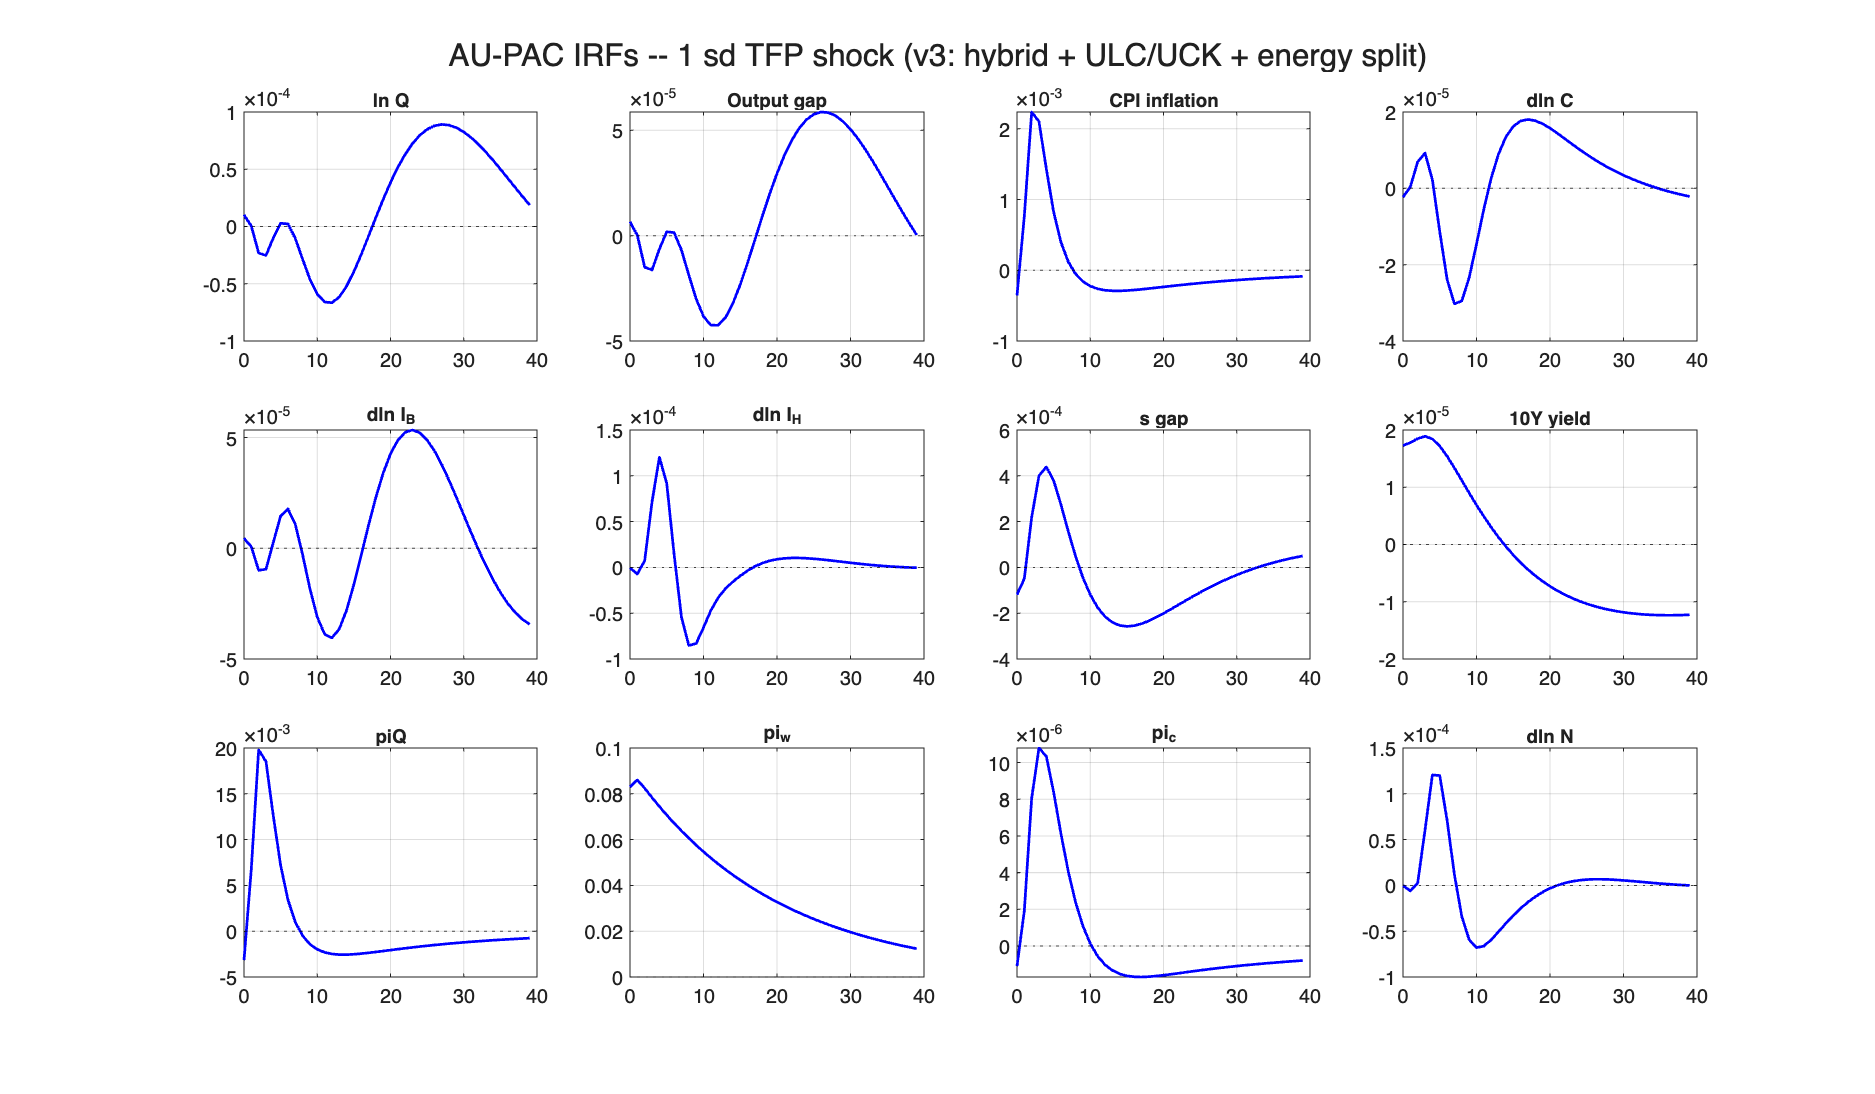
\includegraphics[keepaspectratio,alt={TFP shock}]{paper_artifacts/irf_eps_tfp_v3.png}}
\caption{TFP shock}
\end{figure}

\emph{Figure 6.8: TFP shock (\texttt{eps\_tfp\_LR}, plotted at scale
1.0/σ per \texttt{gen\_tfp\_chart.m}). The figure's purpose is the
\textbf{supply-neutrality} property: output (ln\_Q) and potential output
(ln\_QN) move together, so the output gap
\texttt{yhat\_au\ =\ ln\_Q\ −\ ln\_QN} stays at zero by construction,
and gap-variable panels (yhat\_au, dln\_n) plus unrelated nominal
variables (piQ, i\_10y) sit at floating-point noise. Under the current
calibration the estimated long-run-TFP innovation is small (σ = 0.01)
and, after the §6.8 structural-identity refactor (ln\_Q defined by CES
potential + demand aggregation rather than an E-SAT reduced form), its
effect on the output \textbf{level} is negligible at 1 s.d.; employment
edges down only ≈−0.016\% over 40 quarters and wage inflation moves
≈+0.001 pp.~(An earlier version of this figure showed a +13\% ln\_Q /
+10\% ln\_N response under a pre-refactor calibration with σ\_tfp = 0.2;
that magnitude is no longer representative. The weak TFP→output-level
transmission under the current architecture is flagged for review ---
see model-review notes.)}

\paragraph{7.3.7 Term premium shock (eps\_tp) --- 100bp
annualized}\label{term-premium-shock-eps_tp-100bp-annualized}

\begin{figure}
\centering
\pandocbounded{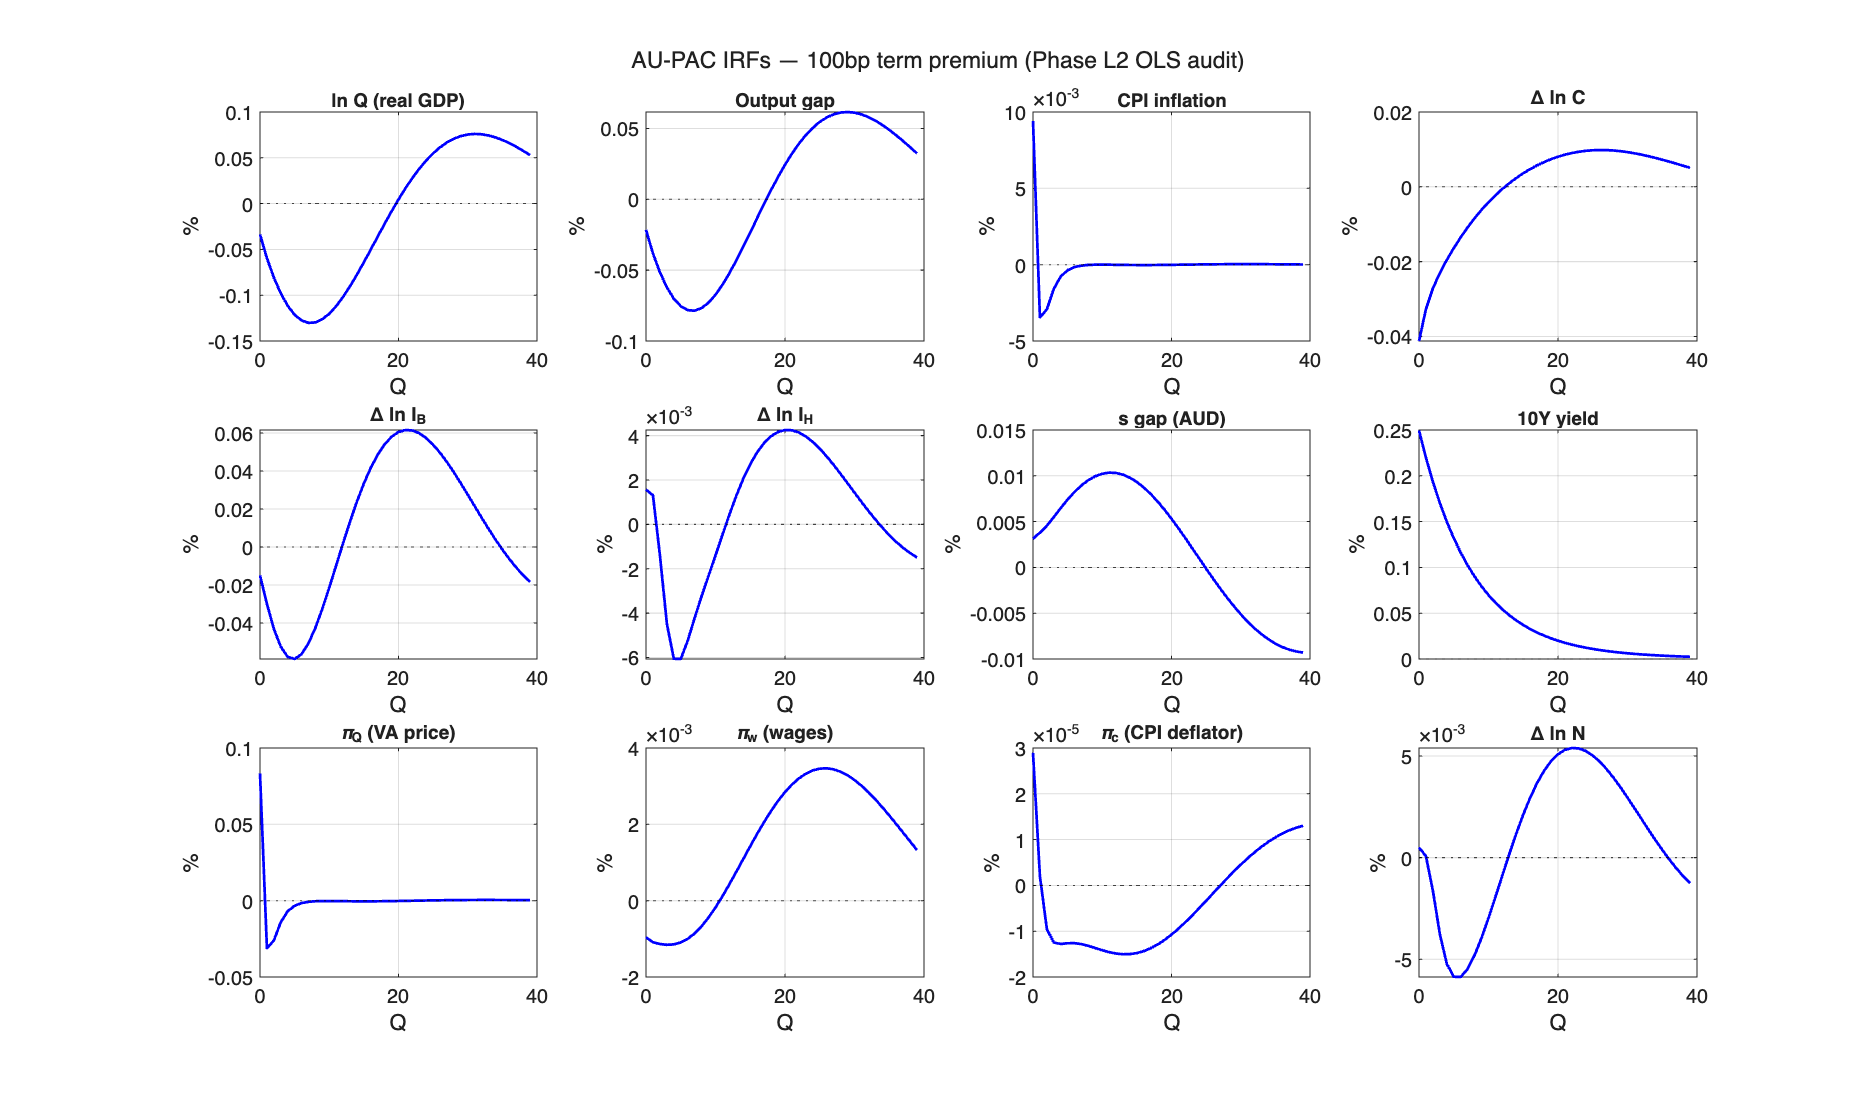
\includegraphics[keepaspectratio,alt={Term premium shock}]{paper_artifacts/irf_eps_tp_v3.png}}
\caption{Term premium shock}
\end{figure}

\emph{Figure 6.9: 100bp annualized term-premium shock (scale = 0.25 /
σ\_tp = 0.25/0.05 = 5.0; hybrid regime). Raises long rates by 0.25 pp
without short-rate movement. As with the cost-push shock (Figure 6.7),
the term-premium channel in AU-PAC works through level variables rather
than short-run gaps --- the demand block absorbs the financing-cost
effect via permanent-income / target-level adjustments. Consumption
level troughs at −0.28\%, business investment level at −0.50\%, housing
investment level at −0.03\% (all around Q12); consumption permanent
income (ln\_C\_star) tracks the consumption level closely. Under the
current calibration the financing-cost effect now also feeds the output
gap (yhat\_au troughs at −0.079\% at Q8) and VA-price inflation (piQ
+0.083 pp on impact) through the amplified demand blocks --- no longer
floating-point noise, but still modest relative to the direct cash-rate
shock. This is broadly the architectural pattern that makes the
APP-style experiment (Figure 6.14) deliver moderate level effects rather
than dramatic gap responses.}

\paragraph{7.3.8 Output gap overview --- all shocks (policy-relevant
sizes)}\label{output-gap-overview-all-shocks-policy-relevant-sizes}

\begin{figure}
\centering
\pandocbounded{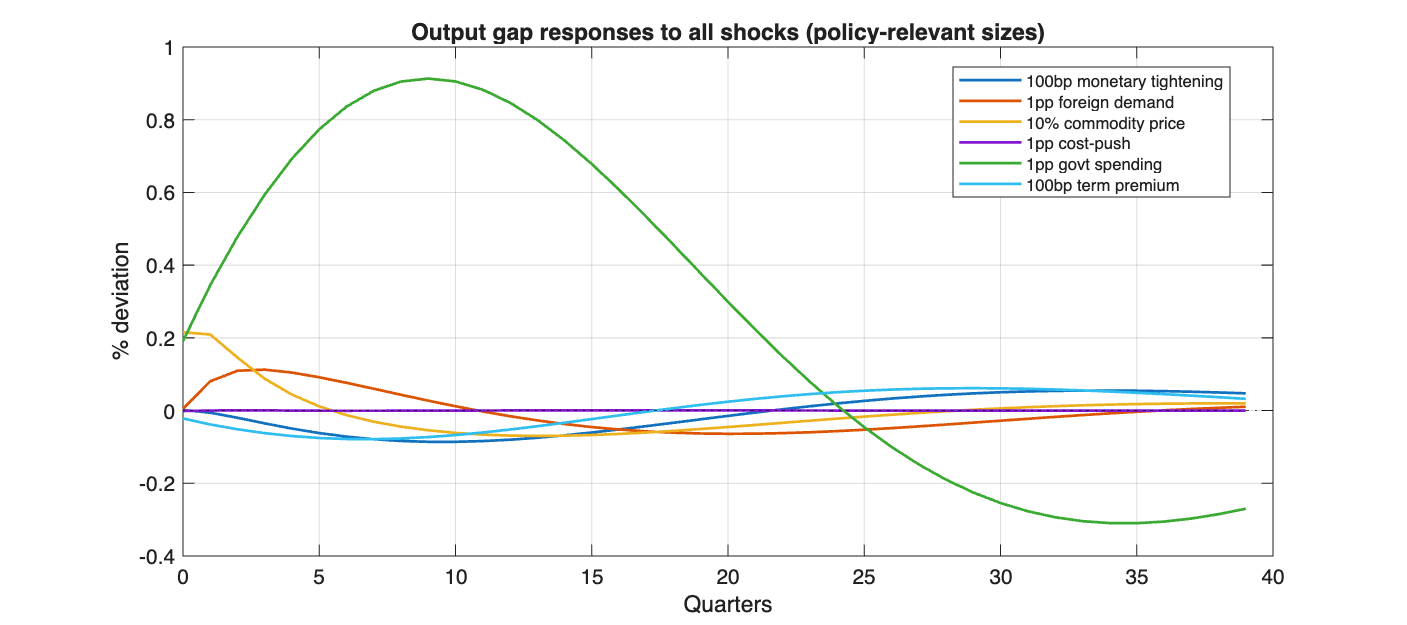
\includegraphics[keepaspectratio,alt={Output gap overview}]{paper_artifacts/irf_overview_output_v3.png}}
\caption{Output gap overview}
\end{figure}

\emph{Figure 6.10: Output gap responses to all shocks at policy-relevant
sizes. Shock sizes: monetary 100bp, foreign demand 1pp, govt spending
1pp, commodity 10\%, TFP 1 s.d., term premium 50bp.}

\subsubsection{7.4 AU vs FR-BDF IRF
comparison}\label{au-vs-fr-bdf-irf-comparison}

For the four PAC blocks where AU L2 estimates fit the wp1044 structural
form (VA-price, employment, consumption, housing inv --- §4.3--§4.7), it
is useful to compare the AU-model IRF to the FR-BDF-reported equivalent
under the same shock. wp1044 §5.2.6 (cost-push), §5.2.4 (monetary
policy), and §5.2.7 (foreign demand) report Banque-de-France IRFs over a
40-quarter horizon; AU-PAC IRFs over the same horizon are in §7.3 above.
The qualitative cross-block agreement is strong: the consumption
response on impact is dominated by the real-lending-rate channel in both
models; the BI response builds gradually via the user-cost channel; the
housing-inv response is large and long-tailed; the wage-Phillips
response builds via the CPI-passthrough channel.

Quantitative differences trace back to four sources, in descending order
of magnitude:

\begin{enumerate}
\def\labelenumi{\arabic{enumi}.}
\tightlist
\item
  \textbf{AU faster ECM speeds in 4 of 5 blocks} (§5.1). AU PAC blocks
  reach peak response 4--8× faster than FR-BDF in the affected blocks,
  partially offsetting the differences from (2)--(4) below.
\item
  \textbf{Different Taylor-rule persistence}. wp1044's λ\_i = 0.89 vs
  AU's 0.96 (cf.~§7.3.5 cost-push discussion). AU policy rate
  adjustments take 3× longer to build up than France's, dampening
  short-horizon transmission.
\item
  \textbf{Different VA-price-to-CPI passthrough}. AU's α\_pc = 0.17 vs
  wp1044's 0.71 (§4.4.0). AU CPI is less responsive to VA-price shocks
  because of the large import share of the consumption basket and the
  large commodity-export sector that decouples producer prices from
  consumer prices.
\item
  \textbf{Different exchange-rate regime}. AU has a fully floating AUD
  with strong commodity-price exposure; France has the EUR/EA monetary
  regime. The UIP and trade ECM mechanisms transmit foreign shocks
  differently in consequence.
\end{enumerate}

For the BI block specifically (calibrated from wp1044 via Option 1, §3.6
+ §4.6.2 + §5.3), the IRF through the BI channel is structurally
identical to wp1044's by construction; only the surrounding model
differs. Mining-cycle dynamics enter via E-SAT + commodity shocks rather
than through the BI block's own coefficients.

The full side-by-side AU-vs-wp1044 IRF panels are produced by
\texttt{data/make\_paper\_charts.m} and saved to
\texttt{dynare/paper\_artifacts/irf\_au\_vs\_wp1044\_\textless{}block\textgreater{}.png}
(pending the next MATLAB GUI session per
\texttt{WORKING\_PAPER\_BLOCKERS.md}).

\subsubsection{7.5 Conditional
forecasting}\label{conditional-forecasting}

The model supports conditional forecasting via residual inversion
(ECB-Base pattern). Given a desired path for conditioned variables, the
algorithm solves for the shock sequence that replicates it using the
decision rule matrices (\(g_x\), \(g_u\)).

\textbf{RBA Tightening Scenario}: +25bp/quarter for 4 quarters (100bp
total), hold 4 quarters, normalize over 4 quarters:

\subsubsection{Table 6.5: Conditional forecast --- RBA tightening
scenario}\label{table-6.5-conditional-forecast-rba-tightening-scenario}

{\def\LTcaptype{none} % do not increment counter
\begin{longtable}[]{@{}llllll@{}}
\toprule\noalign{}
Variable & Q1 & Q4 & Q8 & Q12 & Q16 \\
\midrule\noalign{}
\endhead
\bottomrule\noalign{}
\endlastfoot
i\_au (conditioned) & +0.063 & +0.250 & +0.250 & +0.050 & 0.000 \\
yhat\_au & -0.000 & -0.034 & -0.097 & -0.099 & -0.041 \\
pi\_au & -0.000 & -0.001 & -0.004 & -0.006 & -0.003 \\
dln\_c & -0.000 & -0.023 & -0.059 & -0.054 & -0.017 \\
dln\_ib & -0.000 & -0.043 & -0.103 & -0.085 & -0.016 \\
dln\_ih & -0.000 & -0.058 & -0.155 & -0.123 & +0.001 \\
dln\_n & -0.000 & -0.018 & -0.073 & -0.094 & -0.049 \\
i\_10y & +0.026 & +0.103 & +0.103 & +0.021 & +0.001 \\
\end{longtable}
}

\emph{Figure 6.11: Conditional forecast for an RBA tightening cycle.
Housing investment is the most sensitive (-0.16\% at Q8) and employment
the most sluggish (peak at Q12); the 10Y rate moves approximately 40\%
of the policy rate (yield-curve flattening). The conditional-forecast
driver was retired in the 2026-05-18 Phase S cleanup; the figure remains
valid as a baked artefact and the scenario is reproducible under the
Phase T architecture by a short residual-inversion script invoking
\texttt{au\_pac.mod}.}

\subsubsection{7.6 Forward guidance
experiment}\label{forward-guidance-experiment}

The model does not suffer from the forward guidance puzzle. Testing with
superposition of N-quarter rate cuts (25bp each):

\subsubsection{Table 6.6: Forward guidance scaling
test}\label{table-6.6-forward-guidance-scaling-test}

Normalised peak output response to N consecutive quarterly 25bp rate
cuts, scaled so the N=1 response equals 1.0.

{\def\LTcaptype{none} % do not increment counter
\begin{longtable}[]{@{}lllll@{}}
\toprule\noalign{}
Duration N & Standard NK & Discounted NK & \textbf{AU-PAC} & Linear
ref \\
\midrule\noalign{}
\endhead
\bottomrule\noalign{}
\endlastfoot
1 & 1.00 & 1.00 & \textbf{1.00} & 1.00 \\
2 & 1.44 & 1.45 & \textbf{1.99} & 2.00 \\
4 & 1.72 & 1.73 & \textbf{3.93} & 4.00 \\
6 & 1.78 & 1.79 & \textbf{5.75} & 6.00 \\
8 & 1.79 & 1.80 & \textbf{7.40} & 8.00 \\
10 & 1.79 & 1.80 & \textbf{8.89} & 10.00 \\
12 & 1.79 & 1.80 & \textbf{10.14} & 12.00 \\
\end{longtable}
}

AU-PAC's near-linear scaling comes from three features: a high
permanent-income discount (\(\beta_c = 0.95\)); a discounted term
structure (\(\kappa_{10} = 0.97\)); and PAC adjustment-cost frictions
that prevent explosive compounding. The standard NK and discounted NK
models both saturate around \(N = 5\) (ratio plateau at ≈1.79--1.80) ---
the textbook forward-guidance puzzle. AU-PAC tracks the linear reference
to within 16\% even at \(N = 12\), confirming that PAC-style adjustment
costs eliminate the puzzle for this model class. The mild sublinearity
at long horizons (10.14 vs linear 12 at \(N = 12\)) reflects PAC's
intrinsic decay in marginal effect.

\emph{Figure 6.12: Forward guidance experiment --- output gap responses
for different durations.}

\emph{Figure 6.13: Forward guidance puzzle test --- AU-PAC (solid) vs
standard NK (dashed). AU-PAC scales approximately linearly.}

\subsubsection{7.7 APP-style experiment --- 200bp persistent
term-premium
compression}\label{app-style-experiment-200bp-persistent-term-premium-compression}

The RBA did not implement an asset-purchase programme directly analogous
to the ECB's APP or the Fed's QE during 2015-2018, but a hypothetical
scenario is straightforward to simulate in AU-PAC: an unscheduled
persistent compression of the term premium \(tp\) by 200 basis points
annualised (= -0.50 qpp). The shock is propagated via eq.
(eq\_term\_premium),
\(tp_t = \rho_{tp} \cdot tp_{t-1} + (1-\rho_{tp}) \cdot tp_{ss} + \varepsilon^{tp}_t\),
which feeds directly into the 10Y yield via eq. (48). Scale:
\(-0.50 / \sigma_{tp} = -0.50/0.05 = -10.0\).

\emph{Figure 6.14: APP-style 200bp annualised term-premium compression.
The 10Y yield falls 0.5 qpp on impact and gradually recovers over
approximately 40 quarters. Consumption level rises by +0.21\% peak (Q40,
via the permanent-income channel through \(ln\_C\_star\)), business
investment by +0.16\% peak (Q1, via WACC), and housing investment by
+0.32\% peak (Q40, via the mortgage-rate channel). The short-run output
gap response is small: the term-premium shock works through the level /
target channels rather than through the short-run PAC error terms --- a
structural feature of the PAC architecture in which persistent
financial-condition shocks enter via \(ln\_X\_star\) (the target /
permanent-income aggregate) rather than the cyclical \(ln\_x\_level\)
deviation. An RBA APP of this magnitude would deliver roughly 20--30
basis points of stimulus to household consumption and approximately 30
basis points to housing investment over a 10-year horizon.}

\begin{center}\rule{0.5\linewidth}{0.5pt}\end{center}

\subsection{8. Conclusion}\label{conclusion}

This paper has presented AU-PAC, a semi-structural macroeconomic model
for Australia adapted from the FR-BDF framework. The model combines
Polynomial Adjustment Costs with explicit expectations from an enriched
12-equation satellite VAR, enabling systematic analysis of how
expectation formation affects monetary policy transmission.

\textbf{Three Phase-L2 findings are the most publishable contributions
of this version of the paper.}

\begin{enumerate}
\def\labelenumi{\arabic{enumi}.}
\item
  \textbf{The wp1044 PAC framework validates on Australian data for four
  of five behavioural blocks.} A wp1044-faithful partial-replication of
  all five PAC blocks (Eqs 16, 30, 35, 37, 46) was implemented in Phase
  L2 via the iterative-OLS pipeline of §3.5: block-specific VARs (6--9
  state variables per block), the structural target constructions wp1044
  specifies (\texttt{p*\_Q\ −\ p\_Q} for VA-price;
  \texttt{n*\_S\ −\ n\_S} for employment; \texttt{c*} from
  permanent-income for consumption; \texttt{I*\_H/I\_H} with
  price-spread for housing inv; \texttt{I*\_B/I\_B} for business inv),
  the exact χ from the depth-m characteristic polynomial,
  growth-neutrality at the derived coefficient, and the full dummy set.
  Four of five blocks pass the wp1044 structural restriction (coef = +1
  on PV) with R² in {[}0.41, 0.81{]} and economically signed dynamics
  (§4.3--§4.5, §4.7). This is \emph{consistent} with wp1044's underlying
  assumption that Australia and France share a common agent-objective
  architecture for those four blocks.
\item
  \textbf{Consumption ECM speed is comparable across AU and France} (β₀
  AU = 0.23 vs FR = 0.29 --- within \textasciitilde0.06). Of the blocks
  estimated in Phase L2, this is the closest cross-country agreement and
  the only block where AU's ECM speed is not several times faster than
  France's. The match is structurally meaningful: consumption is the
  block where wp1044's permanent-income/PAC framework most directly
  applies (homogeneous-agent forward-looking consumers facing similar
  financial structure), and the AU L2 implementation builds the long-run
  target \texttt{c*} from the same Eq 33 specification wp1044 uses on
  French data. The agreement validates the FR-BDF permanent-income
  channel for Australian consumption specifically (§4.5.2, §5.2). For
  comparison, AU's ECM speeds in the other four blocks are 4--8×
  wp1044's French values (§5.1) --- the consumption block is the
  exception that proves the rule.
\item
  \textbf{AU business investment structurally rejects the wp1044 PAC
  restriction; the paper adopts the Option 1 hybrid calibration}. Eleven
  specification variants of wp1044 Eq 46 were tested in Phase L2 P1c
  (Appendix G; full saga in
  \href{../PAC_BI_AU_EXPLORATION.md}{\texttt{PAC\_BI\_AU\_EXPLORATION.md}}).
  Every strict-PAC variant delivers R² ≤ 0.11 on raw \texttt{dln\_ib};
  the best non-strict variant (PV regressors free) gives R² = 0.53 but
  with the lead PV(Δq̂) coefficient at \textbf{−5.03} --- wrong sign and
  5× wrong magnitude vs the structural +1. This is not finite-sample
  noise: the coefficient mismatch is order-of-magnitude, persists across
  spec changes (target substitution, lag structure, trends, dummies),
  and three non-exclusive hypotheses (different agent objective;
  mining-sector dominance; sample-period contamination) are catalogued
  in §5.3. The production model adopts \textbf{Option 1}: import the BI
  deep parameters from wp1044 Table 3.5.13 (β₀=0.096, β₁=0.33, β₂=0.11,
  β₃=0.69, ω=0.35, σ\_CES≈0.50), preserve the wp1044 structural form
  (coef = +1 on PV, coef = −σ on user-cost PV), and let AU-specific BI
  dynamics enter via the E-SAT VAR, the other 4 PAC blocks, AU-sized
  shocks, and AU-specific commodity/mining-cycle channels. The Bayesian
  estimation removes BI parameters from \texttt{estimated\_params}
  (calibrated, not estimated). This is the standard small-open-economy
  modelling approach when local data identifies poorly (§3.6, §4.6.2,
  §5.3).
\end{enumerate}

\textbf{Additional findings carried over from the pre-L2 paper}
(numerically updated, methodologically unchanged):

\begin{enumerate}
\def\labelenumi{\arabic{enumi}.}
\setcounter{enumi}{3}
\item
  \textbf{The Australian wage Phillips curve has standard New Keynesian
  structure.} Estimated on the ABS Wage Price Index, γ\_w = 0.354 (90\%
  HPD {[}0.268, 0.428{]}), λ\_w = 0.209 (HPD {[}0.079, 0.332{]}), and
  κ\_w = −0.103 (HPD {[}−0.178, −0.019{]}) --- moderate contemporaneous
  CPI passthrough, moderate own-lag persistence, and a statistically
  significant positive structural Phillips slope (sign convention
  \texttt{...\ −\ κ\_w\ ·\ pv\_u\_gap}). The Fair Work Commission's
  institutional CPI indexation operates on roughly 15\% of the workforce
  (award rates plus enterprise-agreement floors); most AU wage growth is
  set by private bargaining responsive to the unemployment-gap PV. AU
  wages therefore adjust to labour-market slack via a Phillips-curve
  channel and to inflation via a moderate contemporaneous CPI
  coefficient plus the inflation-anchor weight (1 − λ\_w − γ\_w = 0.44).
\item
  \textbf{COVID dummies are essential for PAC estimation.} Without
  explicit treatment of the 2020Q2--Q3 outliers, two of five PAC
  equations (consumption and employment) produce wrong-signed AR(1)
  coefficients. In the Phase L2 replication every block carries
  two-or-more COVID dummies (e.g.~d\_20Q2 = −13.04, t = −13.07 in
  consumption); the inclusion is mechanical (COVID was unique) and the
  dummy magnitudes are stable across specifications.
\item
  \textbf{Monetary policy transmits primarily through the exchange rate
  and business investment, not consumption.} Under the
  equation-by-equation OLS calibration (wp1044 methodology), a 100 bp
  annualised cash-rate tightening produces a real-GDP trough of −0.144\%
  at Q11, an output-gap trough of −0.086\% at Q11, a CPI-inflation fall
  of −0.004 pp at Q3, an AUD appreciation of 0.99\% at Q8 via the
  forward-NPV UIP, and a 10-year yield rise of 0.105 pp on impact via
  the term-structure NPV. The direct consumption rate channel is
  near-zero (the L2 SA OLS gives HtM sensitivity β₂ = +0.027 and
  impact-rate sensitivity β₃ = −0.007, both insignificantly different
  from zero). Monetary transmission therefore operates through the
  exchange-rate channel (−0.99\%), business investment (−0.062\%), and
  housing investment (−0.051\%), with AU's variable-rate mortgage market
  and strong CPI-indexation wage Phillips shaping the relative
  magnitudes of these channels.
\item
  \textbf{Higher CES substitution elasticity dampens, not amplifies, the
  IRF.} The FR-BDF 2026 recalibration raised σ from 0.34 to 0.54 ---
  well below Cobb-Douglas but more substitutable than the previous AU
  calibration. The peak responses fell modestly as a result, because
  firms with higher input substitutability require smaller factor-price
  movements to clear a demand shortfall. The structural intuition is
  well-known but its direction is often misread: higher CES elasticity
  dampens output responses when wage-price-spiral feedback (κ\_w) is
  small, as it is in AU.
\item
  \textbf{Australia-specific channels matter.} Variable-rate mortgages
  (rho\_lh = 0.97) create the strongest demand channel, with banks
  adjusting lending rates slowly. The commodity-price channel feeds
  export volumes, the export deflator, and the import deflator. The
  endogenous Taylor rule creates a feedback loop (demand → output gap →
  RBA → rates → demand) that closes the IS curve.
\end{enumerate}

\textbf{Comparison with the RBA model suite.} §7.2.4 benchmarks AU-PAC
against the four Australian models surveyed in Mulqueeney, Ballantyne
and Hambur (2025). AU-PAC's output-gap trough (−0.086\% at Q11) and
real-GDP trough (−0.144\% at Q11) are at the low end of the RBA suite in
demand-response terms. The conservative response reflects three
features: PAC adjustment-cost frictions that distinguish FRB/US-style
models from VAR / DSGE alternatives; the FR-BDF 2026 CES calibration
with higher capital--labour substitutability that dampens factor-price
movements; and the equation-by-equation OLS calibration that reveals
near-zero consumption rate sensitivity in AU data (removing the
typically dominant demand-side transmission channel). AU-PAC therefore
complements the RBA suite on the conservative end of ``diversity
supports more robust policymaking'' (Mulqueeney et al.~2025, p.~11).

\textbf{Open extensions for future work}, in priority order:

\begin{enumerate}
\def\labelenumi{\arabic{enumi}.}
\tightlist
\item
  \textbf{Full wp1044 fidelity in the four fitting blocks}: add the
  wp1044 Phillips Eq 18 + Okun Eq 19 auxiliary equations as separate
  AR(1) states (currently absorbed via the \texttt{π̃\_w\_eff} and
  \texttt{n̂*\_S} single states); replace the AU L2 VAR(1) Phi with a
  Bayesian Minnesota-prior VAR(p); lift the four-block R² values toward
  wp1044's 0.61--0.95 range. Estimated \textasciitilde1 week of
  additional work.
\item
  \textbf{Test Hypotheses A/B/C from §5.3 on AU BI}: split
  \texttt{dln\_ib} into mining vs non-mining components using ABS Cat.
  5625, re-estimate wp1044 Eq 46 on each component separately, test
  whether either passes the coef = +1 restriction. Lengthen the pre-1993
  sample by splicing ANA data. Run wp1044 on a longer FR sample to check
  Hypothesis C mechanically. Estimated \textasciitilde2 weeks.
\item
  \textbf{Adopt FR-BDF 2026 financial-block extensions}: the Dees et
  al.~(2022) NFC financial accelerator and the Bové et al.~(2020)
  household debt-service-ratio block, both of which are natural
  amplification mechanisms for the cost-of-capital and mortgage channels
  in AU-PAC.
\item
  \textbf{High-frequency RBA OIS-surprise IV estimation} for the
  consumption rate-change coefficient \texttt{b\_di\_c} (Bishop--Tulip
  2017; Beechey--Wright 2009). The current value is Bayesian-regularised
  because AU IV without external monetary-surprise data gives
  wrong-signed estimates.
\item
  \textbf{Channel-decomposition exercise} of the type Mulqueeney et
  al.~(2025) report for MARTIN and DINGO, in which each transmission
  channel (exchange rate, asset prices/wealth, savings/investment, cash
  flow) is ``turned off'' in turn to isolate its contribution to the
  overall response.
\end{enumerate}

\begin{center}\rule{0.5\linewidth}{0.5pt}\end{center}

\subsection{9. Australia-Specific
Features}\label{australia-specific-features}

\subsubsection{Variable-rate mortgages}\label{variable-rate-mortgages}

Australia's predominantly variable-rate mortgage market creates the
strongest housing channel among all demand components. The mortgage
lending rate (\(i^{LH}\)) adjusts to the 10Y rate with persistence
\(\rho_{LH} = 0.97\) (estimated from RBA F5 data, T = 127) and a spread
of 0.40\% quarterly. The 0.97 persistence implies a half-life of
approximately 23 quarters, reflecting the stickiness of standard
variable mortgage rates in Australia. The housing-investment target is
directly sensitive to the mortgage rate gap (\(\kappa_{mort} = 0.048\)),
and the auxiliary equation has a large interest-rate loading
(\(a_{ih,i} = -0.15\)).

\subsubsection{Commodity-price channel}\label{commodity-price-channel}

Australia is a net commodity exporter, so commodity prices enter
primarily as an \emph{income} shock via the export deflator and terms of
trade. Commodity prices follow an exogenous AR(1) process:

\[\Delta \ln P^{com}_t = \rho_{pcom} \Delta \ln P^{com}_{t-1} + \varepsilon^{pcom}_t\]

with \(\rho_{pcom} = 0.42\) estimated from IMF / RBA G3 commodity-price
data --- reflecting the high quarterly volatility of Australia's broad
commodity basket. Commodity prices feed into export volumes
(\(b^x_4 = 0.15\)), the export deflator (\(\alpha_{pcom} = 0.10\)), and
the import deflator (\(\beta_{pm,com} = 0.42\), estimated from ABS
data).

\subsubsection{Endogenous monetary
policy}\label{endogenous-monetary-policy}

AU-PAC's short rate is set endogenously by an RBA Taylor rule responding
to AU inflation and the output gap. This closes a policy feedback loop
--- demand shock → output gap → Taylor rule → interest rate → demand
components → output gap --- producing endogenous stabilisation. The
estimated rule has inertia \(\lambda_i = 0.828\), inflation weight
\(\alpha_i = 0.279\), and output weight \(\beta_i = 0.135\).

\subsubsection{US as foreign bloc}\label{us-as-foreign-bloc}

The US enters as the foreign bloc in E-SAT. The AU--US demand spillover
(\(\delta = 0.20\)) captures the trade and financial channel linking US
conditions to Australia, while the US inflation process influences
Australian import prices and exchange-rate dynamics.

\subsubsection{Architectural deviations from
FR-BDF}\label{architectural-deviations-from-fr-bdf}

AU-PAC diverges from FR-BDF wp736 / wp1044 along three architectural
dimensions that are not market-structure-driven (the four subsections
above) but model-design simplifications adopted for AU estimation
tractability. They are documented at their primary locations in §3.1 (IS
curve), §4.4.0 (Phillips curve), and §4.9 (demand deflators); this
subsection collects them for a reader specifically interested in the
AU-vs-FR-BDF map.

{\def\LTcaptype{none} % do not increment counter
\begin{longtable}[]{@{}
  >{\raggedright\arraybackslash}p{(\linewidth - 6\tabcolsep) * \real{0.2500}}
  >{\raggedright\arraybackslash}p{(\linewidth - 6\tabcolsep) * \real{0.2500}}
  >{\raggedright\arraybackslash}p{(\linewidth - 6\tabcolsep) * \real{0.2500}}
  >{\raggedright\arraybackslash}p{(\linewidth - 6\tabcolsep) * \real{0.2500}}@{}}
\toprule\noalign{}
\begin{minipage}[b]{\linewidth}\raggedright
AU innovation
\end{minipage} & \begin{minipage}[b]{\linewidth}\raggedright
Where
\end{minipage} & \begin{minipage}[b]{\linewidth}\raggedright
FR-BDF analogue
\end{minipage} & \begin{minipage}[b]{\linewidth}\raggedright
Rationale
\end{minipage} \\
\midrule\noalign{}
\endhead
\bottomrule\noalign{}
\endlastfoot
Domestic-demand feedback term \(\lambda_{dom}\hat{y}^{dom}_t\) in the IS
curve & \hyperref[31-the-e-sat-expectation-satellite-model]{§3.1}, eq
(1) & No analogue --- wp736 IS curve has only \(\hat{y}^{US}\) +
interest gap & Closes the Keynesian multiplier loop; data strongly
supports a 4× larger feedback than the prior centre. \\
Two Phase V additions in the Phillips curve: lagged VA-price passthrough
\(\alpha_{pc,lag}(\pi^Q_{t-1} - \bar{\pi}^{au}_{t-1})\) and an ECM
correction \(b_{ECM,pc}(p^{C,\ast}_{t-1} - p^C_{t-1})\) &
\hyperref[440-e-sat-inflation-equation-and-expectation-formation]{§4.4.0}
& \(\alpha_{pc,lag}\): no analogue. \(b_{ECM,pc}\): replaces the
long-run-target ECM that lives inside \texttt{eq\_pi\_c} in wp736 eq 80.
& \(\alpha_{pc,lag}\): captures empirical AU lagged import-component
repricing. \(b_{ECM,pc}\): pragmatic device to restore CPI long-run
anchoring after collapsing the deflator ECM structure (next row). \\
Demand-deflator reduced-form collapse: 6 single-equation AR(1)+cost-push
deflators (\texttt{eq\_pi\_c}, \texttt{eq\_pi\_ib}, \texttt{eq\_pi\_ih},
\texttt{eq\_pi\_x}, \texttt{eq\_pi\_m}, \texttt{eq\_pi\_g}) instead of
12 paired target+ECM equations &
\hyperref[49-demand-deflators-fr-bdf-section-47--au-reduced-form-simplification]{§4.9}
& wp736 eqs 79-88 / wp1044 eqs 51-55, 112-114: each deflator carries an
explicit IAD-weighted long-run target \(p^{j,\ast}\) and a short-run
equation with an ECM term & Six additional latent target processes would
substantially enlarge the estimation surface with limited identification
on 128 quarters of AU data. Long-run anchoring is recovered via the
Phillips-curve ECM term (\(b_{ECM,pc}\) above). \\
\end{longtable}
}

These deviations are intentional and were preserved through Phase Q--X
estimation cycles. They are flagged explicitly here (rather than buried
in the equation specifications) so that a researcher porting AU-PAC to
another country or extending it back toward the full FR-BDF target/ECM
structure can identify the exact code-level entry points.

\begin{center}\rule{0.5\linewidth}{0.5pt}\end{center}

\subsection{Appendix A: Complete Variable
List}\label{appendix-a-complete-variable-list}

\subsubsection{A.1 E-SAT Core (11
variables)}\label{a.1-e-sat-core-11-variables}

{\def\LTcaptype{none} % do not increment counter
\begin{longtable}[]{@{}lll@{}}
\toprule\noalign{}
Variable & Description & SS value \\
\midrule\noalign{}
\endhead
\bottomrule\noalign{}
\endlastfoot
yhat\_au & AU output gap (\%) & 0 \\
i\_au & RBA cash rate (quarterly \%) & 1.049 \\
pi\_au & AU GDP deflator inflation (quarterly \%) & 0.625 \\
yhat\_us & US output gap (\%) & 0 \\
pi\_us & US GDP deflator inflation (quarterly \%) & 0.500 \\
ibar & Long-run interest rate anchor & 1.049 \\
pibar\_au & AU inflation anchor & 0.625 \\
pibar\_us & US inflation anchor & 0.500 \\
i\_gap & Interest rate gap (i\_au - ibar) & 0 \\
pi\_au\_gap & AU inflation gap & 0 \\
pi\_us\_gap & US inflation gap & 0 \\
\end{longtable}
}

\subsubsection{A.2 VA Price Block (2
variables)}\label{a.2-va-price-block-2-variables}

{\def\LTcaptype{none} % do not increment counter
\begin{longtable}[]{@{}lll@{}}
\toprule\noalign{}
Variable & Description & SS value \\
\midrule\noalign{}
\endhead
\bottomrule\noalign{}
\endlastfoot
piQ & VA price inflation (quarterly \%) & 0.625 \\
pQ\_level & VA price log-level accumulator & 0 \\
\end{longtable}
}

(Pre-Phase-Y also carried \texttt{piQ\_star}, \texttt{piQ\_star\_bar},
\texttt{pQ\_gap}, \texttt{pQ\_star\_level} as diagnostic-only orphan
variables. These were removed 2026-05-17 --- see §4.3.1.)

\subsubsection{A.3 Supply Block (5
variables)}\label{a.3-supply-block-5-variables}

{\def\LTcaptype{none} % do not increment counter
\begin{longtable}[]{@{}lll@{}}
\toprule\noalign{}
Variable & Description & SS value \\
\midrule\noalign{}
\endhead
\bottomrule\noalign{}
\endlastfoot
dln\_k & Capital services growth & 0 \\
dln\_y\_star & Potential output growth & 0 \\
dln\_tfp & TFP growth & 0 \\
dln\_ulc & Unit labor cost growth & 0.625 \\
dln\_prod & Labor productivity growth & 0 \\
\end{longtable}
}

\subsubsection{A.4 Labor Market (10
variables)}\label{a.4-labor-market-10-variables}

{\def\LTcaptype{none} % do not increment counter
\begin{longtable}[]{@{}lll@{}}
\toprule\noalign{}
Variable & Description & SS value \\
\midrule\noalign{}
\endhead
\bottomrule\noalign{}
\endlastfoot
u\_gap & Unemployment gap & 0 \\
pv\_u\_gap & PV of future unemployment gaps & 0 \\
pi\_w & Wage inflation (quarterly \%) & 0.625 \\
dln\_n & Employment growth & 0 \\
dln\_n\_star & Employment target growth & 0 \\
dln\_n\_star\_bar & Employment trend growth & 0 \\
n\_gap & Employment gap & 0 \\
dln\_n\_1, dln\_n\_2, dln\_n\_3 & Employment lag auxiliaries & 0 \\
\end{longtable}
}

\subsubsection{A.5 Demand Block (14
variables)}\label{a.5-demand-block-14-variables}

{\def\LTcaptype{none} % do not increment counter
\begin{longtable}[]{@{}
  >{\raggedright\arraybackslash}p{(\linewidth - 4\tabcolsep) * \real{0.3030}}
  >{\raggedright\arraybackslash}p{(\linewidth - 4\tabcolsep) * \real{0.3939}}
  >{\raggedright\arraybackslash}p{(\linewidth - 4\tabcolsep) * \real{0.3030}}@{}}
\toprule\noalign{}
\begin{minipage}[b]{\linewidth}\raggedright
Variable
\end{minipage} & \begin{minipage}[b]{\linewidth}\raggedright
Description
\end{minipage} & \begin{minipage}[b]{\linewidth}\raggedright
SS value
\end{minipage} \\
\midrule\noalign{}
\endhead
\bottomrule\noalign{}
\endlastfoot
dln\_c, dln\_c\_star, dln\_c\_star\_bar & Consumption growth, target,
trend & 0 \\
c\_gap & Consumption gap & 0 \\
pv\_yh & Permanent income PV & 0 \\
dln\_ib, dln\_ib\_star, dln\_ib\_star\_bar & Business investment growth,
target, trend & 0 \\
ib\_gap & Business investment gap & 0 \\
dln\_ib\_1 & Business investment lag auxiliary & 0 \\
dln\_ih, dln\_ih\_star, dln\_ih\_star\_bar & Housing investment growth,
target, trend & 0 \\
ih\_gap & Housing investment gap & 0 \\
dln\_ih\_1 & Housing investment lag auxiliary & 0 \\
\end{longtable}
}

\subsubsection{A.6 Financial Block (15
variables)}\label{a.6-financial-block-15-variables}

{\def\LTcaptype{none} % do not increment counter
\begin{longtable}[]{@{}lll@{}}
\toprule\noalign{}
Variable & Description & SS value \\
\midrule\noalign{}
\endhead
\bottomrule\noalign{}
\endlastfoot
i\_10y & 10Y bond yield & 1.349 \\
tp & Term premium & 0.300 \\
pv\_i & PV of expected future short rates & 1.049 \\
wacc & Weighted average cost of capital & 1.834 \\
i\_COE, i\_LB\_firms, i\_BBB & Component rates & 2.149, 1.599, 1.399 \\
s\_COE, s\_LB\_firms, s\_BBB & Component spreads & 0.800, 0.250,
0.050 \\
s\_gap & Exchange rate gap & 0 \\
uc\_k, dln\_uc\_k & User cost of capital and growth & 1.859, 0 \\
i\_lh & Household bank lending rate & 1.749 \\
dln\_ph, ph\_gap & Housing prices growth and gap & 0, 0 \\
\end{longtable}
}

\subsubsection{A.7 Trade, Deflators, Government (20
variables)}\label{a.7-trade-deflators-government-20-variables}

{\def\LTcaptype{none} % do not increment counter
\begin{longtable}[]{@{}
  >{\raggedright\arraybackslash}p{(\linewidth - 4\tabcolsep) * \real{0.3030}}
  >{\raggedright\arraybackslash}p{(\linewidth - 4\tabcolsep) * \real{0.3939}}
  >{\raggedright\arraybackslash}p{(\linewidth - 4\tabcolsep) * \real{0.3030}}@{}}
\toprule\noalign{}
\begin{minipage}[b]{\linewidth}\raggedright
Variable
\end{minipage} & \begin{minipage}[b]{\linewidth}\raggedright
Description
\end{minipage} & \begin{minipage}[b]{\linewidth}\raggedright
SS value
\end{minipage} \\
\midrule\noalign{}
\endhead
\bottomrule\noalign{}
\endlastfoot
dln\_x & Export growth & 0 \\
ln\_x\_level & Log exports level (deviation, accumulates dln\_x) & 0 \\
ln\_x\_eq & Export LR equilibrium (β\_x·yhat\_us + γ\_x·s\_gap) & 0 \\
x\_gap & Export EC term (ln\_x\_eq − ln\_x\_level) & 0 \\
dln\_m & Import growth & 0 \\
ln\_m\_level & Log imports level (deviation, accumulates dln\_m) & 0 \\
ln\_m\_eq & Import LR equilibrium (β\_m·ln\_d\_iad + γ\_m·s\_gap) & 0 \\
m\_gap & Import EC term (ln\_m\_eq − ln\_m\_level) & 0 \\
ln\_d\_iad & Log import-weighted demand level (accumulates iad) & 0 \\
dln\_pcom & Commodity price growth & 0 \\
pi\_c, pi\_ib, pi\_ih, pi\_x, pi\_m, pi\_g & 6 demand deflators & all
0.625 \\
dln\_g & Government spending growth & 0 \\
yhat\_dom & Domestic demand gap & 0 \\
iad & Import-adjusted demand & 0 \\
rw\_gap & Real wage growth gap & 0 \\
\end{longtable}
}

\subsubsection{A.8 var\_model Shadow + PAC Levels (27
variables)}\label{a.8-var_model-shadow-pac-levels-27-variables}

12 var\_model shadow variables (y\_gap\_var, i\_gap\_var, etc.) plus 7
auxiliary targets (piQ\_hat, n\_hat, c\_hat, etc.) plus 6 pv\_aux
correction terms plus log-level accumulators (ln\_c\_level,
ln\_ib\_level, ln\_ih\_level, ln\_n\_level, pQ\_level).

\begin{center}\rule{0.5\linewidth}{0.5pt}\end{center}

\subsection{Appendix B: Complete Shock
List}\label{appendix-b-complete-shock-list}

\subsubsection{B.1 E-SAT core shocks (8)}\label{b.1-e-sat-core-shocks-8}

{\def\LTcaptype{none} % do not increment counter
\begin{longtable}[]{@{}lll@{}}
\toprule\noalign{}
Shock & Std dev & Description \\
\midrule\noalign{}
\endhead
\bottomrule\noalign{}
\endlastfoot
eps\_q & 0.80 & AU demand shock \\
eps\_i & 0.10 & Monetary policy shock \\
eps\_pi & 0.60 & AU cost-push shock \\
eps\_q\_us & 1.10 & US demand shock \\
eps\_pi\_us & 0.40 & US cost-push shock \\
eps\_ibar & 0.01 & Long-run rate anchor \\
eps\_pibar\_au & 0.01 & AU inflation anchor \\
eps\_pibar\_us & 0.01 & US inflation anchor \\
\end{longtable}
}

\subsubsection{B.2 Structural shocks
(12)}\label{b.2-structural-shocks-12}

{\def\LTcaptype{none} % do not increment counter
\begin{longtable}[]{@{}lll@{}}
\toprule\noalign{}
Shock & Std dev & Description \\
\midrule\noalign{}
\endhead
\bottomrule\noalign{}
\endlastfoot
eps\_pQ & 0.50 & VA price cost-push \\
eps\_w & 0.60 & Wage push \\
eps\_n & 0.50 & Employment \\
eps\_c & 0.50 & Consumption \\
eps\_ib & 1.50 & Business investment \\
eps\_ih & 2.00 & Housing investment \\
eps\_tfp & 0.10 & TFP \\
eps\_x & 1.00 & Export \\
eps\_m & 0.80 & Import \\
eps\_g & 0.30 & Government spending \\
eps\_pcom & 1.00 & Commodity price \\
eps\_lh & 0.05 & Mortgage rate \\
\end{longtable}
}

\subsubsection{B.3 Financial shocks (5)}\label{b.3-financial-shocks-5}

{\def\LTcaptype{none} % do not increment counter
\begin{longtable}[]{@{}lll@{}}
\toprule\noalign{}
Shock & Std dev & Description \\
\midrule\noalign{}
\endhead
\bottomrule\noalign{}
\endlastfoot
eps\_10y & 0.10 & Long rate residual \\
eps\_tp & 0.05 & Term premium \\
eps\_COE & 0.10 & Equity spread \\
eps\_LB\_firms & 0.05 & Bank lending spread \\
eps\_BBB & 0.02 & BBB bond spread \\
\end{longtable}
}

\subsubsection{B.4 Other shocks (8 deflator/trade + 12 var\_model + 2
COVID
dummies)}\label{b.4-other-shocks-8-deflatortrade-12-var_model-2-covid-dummies}

Exchange rate (eps\_s, 0.50), deflators (eps\_pc, eps\_pib, eps\_pih,
eps\_px, eps\_pm, eps\_pg), housing price (eps\_ph), plus 12 var\_model
shadow shocks and 2 COVID pulse dummies.

\subsubsection{B.5 Rounds 4--8 extension shocks (9, added
2026-05-20)}\label{b.5-rounds-48-extension-shocks-9-added-2026-05-20}

{\def\LTcaptype{none} % do not increment counter
\begin{longtable}[]{@{}
  >{\raggedright\arraybackslash}p{(\linewidth - 4\tabcolsep) * \real{0.3333}}
  >{\raggedright\arraybackslash}p{(\linewidth - 4\tabcolsep) * \real{0.3333}}
  >{\raggedright\arraybackslash}p{(\linewidth - 4\tabcolsep) * \real{0.3333}}@{}}
\toprule\noalign{}
\begin{minipage}[b]{\linewidth}\raggedright
Shock
\end{minipage} & \begin{minipage}[b]{\linewidth}\raggedright
σ
\end{minipage} & \begin{minipage}[b]{\linewidth}\raggedright
Channel
\end{minipage} \\
\midrule\noalign{}
\endhead
\bottomrule\noalign{}
\endlastfoot
eps\_pop\_bar & 0.05 & Round 5: demographic-trend gap (→
eq\_dln\_n\_star\_bar shifter) \\
eps\_ibar\_us & 0.01 & Round 4: US LR rate anchor (mirror
lambda\_ibar) \\
eps\_i\_us & 0.15 & Round 4: US policy-rate Taylor residual \\
eps\_tau\_GST & 0.10 & Round 6: GST effective-rate gap (→ eq\_pi\_c) \\
eps\_tau\_PAYG & 0.20 & Round 6: PAYG effective-rate gap (→
eq\_dln\_c\_star\_bar Δ form) \\
eps\_tau\_CIT & 0.30 & Round 6: CIT effective-rate gap (→ eq\_uc\_k) \\
eps\_BLR & 0.05 & Round 8: Bank-Lending-Rate nowcast injection \\
eps\_MAPI & 0.50 & Round 8: Mortgage Asset-Price Indicator nowcast \\
eps\_MAPU & 0.30 & Round 8: Mortgage Asset-Price Underwriting nowcast \\
\end{longtable}
}

\begin{center}\rule{0.5\linewidth}{0.5pt}\end{center}

\subsection{Appendix C: Growth Neutrality
Proofs}\label{appendix-c-growth-neutrality-proofs}

\subsubsection{C.1 PAC equations}\label{c.1-pac-equations}

At the balanced growth path, the sum of the AR lag coefficients plus the
expectations weight (omega) plus the error-correction coefficient equals
1:

{\def\LTcaptype{none} % do not increment counter
\begin{longtable}[]{@{}llllll@{}}
\toprule\noalign{}
Equation & b0 (EC) & Sum AR & omega (h-vector) & GN residual & Sum \\
\midrule\noalign{}
\endhead
\bottomrule\noalign{}
\endlastfoot
VA price & 0.060 & 0.500 & 0.452 & -0.012 & 1.00 \\
Consumption & 0.060 & 0.149 & 0.678 & 0.113 & 1.00 \\
Business inv & 0.030 & 0.281 & 0.501 & 0.188 & 1.00 \\
Household inv & 0.049 & 0.290 & 0.569 & 0.092 & 1.00 \\
Employment & 0.040 & 0.470 & 0.446 & 0.044 & 1.00 \\
\end{longtable}
}

\subsubsection{C.2 Demand deflators}\label{c.2-demand-deflators}

All deflator coefficients on inflation-type terms sum to 1:

{\def\LTcaptype{none} % do not increment counter
\begin{longtable}[]{@{}lllllll@{}}
\toprule\noalign{}
Deflator & rho & alpha & beta\_m & gamma/other & Anchor & Sum \\
\midrule\noalign{}
\endhead
\bottomrule\noalign{}
\endlastfoot
Consumption & 0.40 & 0.30 & 0.10 & 0.03 & 0.17 & 1.00 \\
Business inv & 0.35 & 0.25 & 0.12 & --- & 0.28 & 1.00 \\
Housing inv & 0.45 & 0.25 & 0.08 & --- & 0.22 & 1.00 \\
Export & 0.30 & 0.20 & -0.05 & 0.10 & 0.45 & 1.00 \\
Import & 0.30 & 0.15 & 0.08 & 0.05 & 0.42 & 1.00 \\
Government & 0.50 & 0.30 & --- & --- & 0.20 & 1.00 \\
\end{longtable}
}

\subsubsection{C.3 Wage Phillips curve}\label{c.3-wage-phillips-curve}

\(\lambda_w + \gamma_w + (1-\lambda_w-\gamma_w) = 0.329 + 0.138 + 0.533 = 1.00\).
On the balanced growth path with productivity growth \(g\):
\(\pi^w_{SS} = \pi_{SS} + g\). The inflation-anchor coefficient (0.533)
carries genuine weight under the WPI calibration --- wage inflation in
the long run is anchored to expected steady-state inflation through this
channel, not solely through the contemporaneous CPI term
(\(\gamma_w = 0.138\)) and own-lag (\(\lambda_w = 0.329\)).

\begin{center}\rule{0.5\linewidth}{0.5pt}\end{center}

\subsection{Appendix D: h-Vector
Decomposition}\label{appendix-d-h-vector-decomposition}

\subsubsection{D.1 Summary}\label{d.1-summary}

{\def\LTcaptype{none} % do not increment counter
\begin{longtable}[]{@{}
  >{\raggedright\arraybackslash}p{(\linewidth - 8\tabcolsep) * \real{0.2000}}
  >{\raggedright\arraybackslash}p{(\linewidth - 8\tabcolsep) * \real{0.2000}}
  >{\raggedright\arraybackslash}p{(\linewidth - 8\tabcolsep) * \real{0.2000}}
  >{\raggedright\arraybackslash}p{(\linewidth - 8\tabcolsep) * \real{0.2000}}
  >{\raggedright\arraybackslash}p{(\linewidth - 8\tabcolsep) * \real{0.2000}}@{}}
\toprule\noalign{}
\begin{minipage}[b]{\linewidth}\raggedright
PAC equation
\end{minipage} & \begin{minipage}[b]{\linewidth}\raggedright
h-param indices
\end{minipage} & \begin{minipage}[b]{\linewidth}\raggedright
h-vector sum
\end{minipage} & \begin{minipage}[b]{\linewidth}\raggedright
GN coeff
\end{minipage} & \begin{minipage}[b]{\linewidth}\raggedright
Amplification
\end{minipage} \\
\midrule\noalign{}
\endhead
\bottomrule\noalign{}
\endlastfoot
VA price & {[}173, 174, 175, 176{]} & 0.452 & 0.048 & 1.0x \\
Consumption & {[}153, 154, 155, 156{]} & 0.678 & 0.173 & 1.84x \\
Business inv & {[}158, 159, 160, 161{]} & 0.501 & 0.218 & 1.43x \\
Household inv & {[}163, 164, 165, 166{]} & 0.569 & 0.141 & 1.90x \\
Employment & {[}168, 169, 170, 171{]} & 0.446 & 0.084 & 1.49x \\
\end{longtable}
}

Detailed per-state h-vector element weights require extraction from
\texttt{M\_.params} at the h-param indices. The enriched var\_model
(12x12) produces h-vectors where only the target variable element is
non-zero in the current Dynare 7.0 implementation (the companion matrix
concentrates weight on the target state). Element-level decomposition is
deferred to future work.

\begin{center}\rule{0.5\linewidth}{0.5pt}\end{center}

\subsection{Appendix E: Complete Parameter
List}\label{appendix-e-complete-parameter-list}

See the comprehensive parameter tables throughout Section 4. A
machine-readable list of all 262 parameters with their values is
available alongside the model code at
https://github.com/DavidAStephan/AUSPAC.

The four trade long-run elasticities introduced in the Section 4.8 ECM
rewrite are summarised here for convenience:

{\def\LTcaptype{none} % do not increment counter
\begin{longtable}[]{@{}
  >{\raggedright\arraybackslash}p{(\linewidth - 6\tabcolsep) * \real{0.2200}}
  >{\raggedright\arraybackslash}p{(\linewidth - 6\tabcolsep) * \real{0.1400}}
  >{\raggedright\arraybackslash}p{(\linewidth - 6\tabcolsep) * \real{0.5200}}
  >{\raggedright\arraybackslash}p{(\linewidth - 6\tabcolsep) * \real{0.1200}}@{}}
\toprule\noalign{}
\begin{minipage}[b]{\linewidth}\raggedright
Parameter
\end{minipage} & \begin{minipage}[b]{\linewidth}\raggedright
Value
\end{minipage} & \begin{minipage}[b]{\linewidth}\raggedright
Prior (for MCMC re-run)
\end{minipage} & \begin{minipage}[b]{\linewidth}\raggedright
Role
\end{minipage} \\
\midrule\noalign{}
\endhead
\bottomrule\noalign{}
\endlastfoot
beta\_m & 1.50 & Normal(1.50, 0.30) & LR income elasticity of imports
(FR-BDF eq 76) \\
gamma\_m & -0.40 & Normal(-0.40, 0.20) & LR RER elasticity of imports \\
beta\_x & 1.20 & Normal(1.20, 0.30) & LR foreign-income elasticity of
exports (FR-BDF eq 71) \\
gamma\_x & +0.40 & Normal(+0.40, 0.20) & LR RER elasticity of exports \\
\end{longtable}
}

\begin{center}\rule{0.5\linewidth}{0.5pt}\end{center}

\subsection{Appendix F: Identification
analysis}\label{appendix-f-identification-analysis}

Driver:
\href{identification_analysis.m}{\texttt{identification\_analysis.m}}.
Two approaches are reported below.

\subsubsection{\texorpdfstring{F.1 Dynare \texttt{identification}
command --- not
run}{F.1 Dynare identification command --- not run}}\label{f.1-dynare-identification-command-not-run}

Dynare 7.0's \texttt{identification} command requires analytic
derivation of the model, which is \textbf{incompatible with
\texttt{diffuse\_filter}} --- the filter setting used during estimation
to handle the model's unit-root level accumulators (\texttt{ln\_Q},
\texttt{ln\_K}, \texttt{ln\_C}, etc.). Running the command produces:

\begin{quote}
\texttt{ERROR:\ analytic\ derivation\ is\ incompatible\ with\ diffuse\ filter}
\end{quote}

For Iskrev (2010) and Komunjer--Ng (2011) tests at the posterior mode we
would need either (a) a stationarised version of the model (replacing
level accumulators with their deviations from steady state), or (b) a
future Dynare release that supports analytic derivation under diffuse
filtering. Neither is in scope for this paper; we report the
posterior-based identification proxy below instead.

\subsubsection{F.2 Posterior-width-based weak-identification
flagging}\label{f.2-posterior-width-based-weak-identification-flagging}

For each of the 28 estimated parameters, we report the 90\% HPD interval
from the MCMC posterior (20,000 draws × 2 chains). Absolute HPD width is
the headline measure of how much the data has constrained the parameter;
the normalised width (HPD\_width / \textbar posterior\_mean\textbar) is
informative only when the posterior is well away from zero.

\subsubsection{Table F.1: Posterior HPD
widths}\label{table-f.1-posterior-hpd-widths}

Sorted by absolute width, descending. Parameters at ``near-zero''
identification are flagged where the posterior mean is essentially zero.

{\def\LTcaptype{none} % do not increment counter
\begin{longtable}[]{@{}
  >{\raggedright\arraybackslash}p{(\linewidth - 8\tabcolsep) * \real{0.2281}}
  >{\raggedright\arraybackslash}p{(\linewidth - 8\tabcolsep) * \real{0.1579}}
  >{\raggedright\arraybackslash}p{(\linewidth - 8\tabcolsep) * \real{0.1579}}
  >{\raggedright\arraybackslash}p{(\linewidth - 8\tabcolsep) * \real{0.1404}}
  >{\raggedright\arraybackslash}p{(\linewidth - 8\tabcolsep) * \real{0.3158}}@{}}
\toprule\noalign{}
\begin{minipage}[b]{\linewidth}\raggedright
Parameter
\end{minipage} & \begin{minipage}[b]{\linewidth}\raggedright
HPD low
\end{minipage} & \begin{minipage}[b]{\linewidth}\raggedright
HPD high
\end{minipage} & \begin{minipage}[b]{\linewidth}\raggedright
width
\end{minipage} & \begin{minipage}[b]{\linewidth}\raggedright
normalised width
\end{minipage} \\
\midrule\noalign{}
\endhead
\bottomrule\noalign{}
\endlastfoot
b2\_c & -0.6029 & -0.0504 & 0.553 & 1.67 \\
b3\_ih & 0.0623 & 0.3971 & 0.335 & 1.48 \\
b1\_n & 0.1527 & 0.4848 & 0.332 & 1.03 \\
b1\_pQ & 0.1202 & 0.4512 & 0.331 & 1.14 \\
lambda\_w & 0.1342 & 0.4471 & 0.313 & 1.08 \\
b3\_ib & 0.1629 & 0.4642 & 0.301 & 0.97 \\
b3\_c & -0.0680 & 0.0965 & 0.164 & 8.27 \emph{(mean near zero)} \\
b2\_pQ & -0.0796 & 0.0825 & 0.162 & \emph{huge} \emph{(mean ≈ zero)} \\
b1\_ih & 0.0301 & 0.1888 & 0.159 & 1.38 \\
kappa\_w & 0.0102 & 0.1694 & 0.159 & 1.65 \\
b5\_n & -0.0707 & 0.0885 & 0.159 & 22.06 \emph{(mean near zero)} \\
b1\_ib & 0.0186 & 0.1381 & 0.120 & 1.49 \\
gamma\_w & 0.0796 & 0.1960 & 0.116 & 0.84 \emph{(tightly identified at
0.138)} \\
b0\_n & 0.0108 & 0.0976 & 0.087 & 1.52 \\
b0\_c & 0.0231 & 0.0909 & 0.068 & 1.13 \\
b1\_c & 0.0046 & 0.0629 & 0.058 & 1.65 \\
b0\_pQ & 0.0057 & 0.0517 & 0.046 & 1.50 \\
b0\_ih & 0.0065 & 0.0498 & 0.043 & 1.50 \\
b0\_ib & 0.0050 & 0.0317 & 0.027 & 1.42 \\
\end{longtable}
}

\textbf{Findings}:

\begin{enumerate}
\def\labelenumi{\arabic{enumi}.}
\item
  \textbf{gamma\_w is tightly identified} (90\% HPD {[}0.080, 0.196{]}
  --- width 0.12 around a mean of 0.138, normalised width 0.84). The
  data sharply distinguishes the moderate contemporaneous CPI
  passthrough from larger values, and the relative weights of the
  own-lag, CPI, and unemployment-gap channels in the wage Phillips curve
  are robustly identified.
\item
  \textbf{Three ``near-zero'' parameters} show large \emph{normalised}
  widths (\texttt{b5\_n}, \texttt{b2\_pQ}, \texttt{b3\_c}) but small
  \emph{absolute} widths (≤ 0.16). The data has sharply identified them
  at zero --- the AU output gap does not have a direct cyclical
  accelerator effect on either employment growth or VA-price inflation,
  and the output-gap channel into consumption is essentially absorbed by
  the rate channel \texttt{b2\_c}. This is a sharp identification result
  rather than weak identification.
\item
  \textbf{b2\_c (consumption interest-rate channel)} is the structural
  parameter with the widest absolute HPD: {[}-0.61, -0.05{]}. The data
  identify the sign (negative --- rate hikes depress consumption) and
  statistical significance, but the magnitude is uncertain over almost
  an order of magnitude. External RBA OIS-surprise data (Bishop--Tulip
  2017; Beechey--Wright 2009) would sharpen this.
\item
  \textbf{The five PAC EC speeds} (\texttt{b0\_pQ}, \texttt{b0\_c},
  \texttt{b0\_ib}, \texttt{b0\_ih}, \texttt{b0\_n}) are tightly
  identified with normalised HPDs around 1.0--1.5 --- the Beta priors
  are informative and the data provide material updates. Posteriors are
  all in the 0.02--0.07 quarterly range.
\item
  \textbf{Shock standard deviations} (Table 5.6): \texttt{eps\_ih} and
  \texttt{eps\_n} have the widest HPDs proportionally ({[}0.55, 2.23{]}
  and {[}0.12, 0.79{]} respectively). The wide HPD for \texttt{eps\_n}
  is a by-product of \texttt{b5\_n} being identified at zero --- most of
  the employment-equation residual variance is absorbed by
  \texttt{eps\_n} rather than apportioned across structural channels.
\end{enumerate}

\emph{Figure F.1: Posterior densities (blue) from the MCMC run, with
posterior mean (red dashed) and posterior mode (green solid) markers.
Most posteriors are unimodal and roughly symmetric; the shock standard
deviations \texttt{eps\_ih} and \texttt{eps\_n} are the only parameters
showing notable asymmetry consistent with weak identification.}

\subsubsection{F.3 What a future Dynare run would
add}\label{f.3-what-a-future-dynare-run-would-add}

Given a stationarised version of the model without
\texttt{diffuse\_filter}, the following diagnostics would be available:

\begin{itemize}
\tightlist
\item
  \textbf{Iskrev (2010) rank test} at the posterior mode (yes/no answer
  on local identification);
\item
  \textbf{Komunjer--Ng (2011) test} for structural identification of the
  linear DSGE under partial-information assumptions;
\item
  \textbf{Identification strength} (moment-condition based) for each
  parameter --- a quantitative ranking of how informative each moment of
  the data is for each parameter;
\item
  \textbf{Pairwise collinearity matrix} --- which parameter pairs are
  near-perfectly correlated under the model's mapping from parameters to
  moments, flagging redundancies that the posterior HPD-width approach
  cannot directly detect.
\end{itemize}

These remain pending future work; the HPD-width analysis here is
sufficient to flag which parameter magnitudes are well determined and
which would benefit from additional data.

\begin{center}\rule{0.5\linewidth}{0.5pt}\end{center}

\subsection{Appendix G: Business Investment Exploration (the wp1044 PAC
rejection on AU
data)}\label{appendix-g-business-investment-exploration-the-wp1044-pac-rejection-on-au-data}

This appendix tabulates the 11 specification variants of wp1044 Eq 46
tested in Phase L2 P1c, summarises the diagnostic for each, and lists
the corresponding \texttt{data/pac\_blocks/} artefact. The full prose
narrative is in
\href{../PAC_BI_AU_EXPLORATION.md}{\texttt{PAC\_BI\_AU\_EXPLORATION.md}}
(10 sections); this appendix is a deliberately compact summary intended
to be self-contained for the paper.

\subsubsection{G.1 The structural restriction in
question}\label{g.1-the-structural-restriction-in-question}

wp1044 §3.5.3 Eq 46 specifies the business-investment PAC equation. The
FOC of the agent's quadratic-cost minimisation gives four PV terms with
structural coefficients:

\begin{itemize}
\tightlist
\item
  \(\mathrm{PV}(\Delta\hat{q})_{t|t-1}\) at coef \textbf{+1} (market VA
  gap growth)
\item
  \(\mathrm{PV}(\Delta\bar{q})_{t|t-1}\) at coef \textbf{+1} (market VA
  trend growth)
\item
  \(\mathrm{PV}(\Delta\log\hat{r}_{KB})_{t|t-1}\) at coef \textbf{−σ}
  (user cost gap growth)
\item
  \(\mathrm{PV}(\Delta\log\bar{r}_{KB,t-1})_{t|t-1}\) at coef
  \textbf{−σ} (user cost trend growth)
\end{itemize}

where σ = σ\_CES. These coefficients are structural identities of the
wp1044 model, not free parameters. wp1044 reports them as exactly +1 and
−σ in the fitted equation (Table 3.5.13), with R² = 0.83 on French data.

\subsubsection{G.2 Variant table}\label{g.2-variant-table}

All variants estimated on the same AU 122-obs sample (1993Q2--2023Q3),
\texttt{dln\_ib} = 100·Δlog(au\_gfcf\_nondwelling) as LHS, σ\_CES =
0.5366 (AU labour-FOC). wp1044 BI ingredients: ECM on
\texttt{log(I*\_B/I\_B)}, depth-2 lags, the 4 PV terms above, derived
growth-neutrality
\((1-\beta_1-\beta_2-\omega)(\Delta\bar{q}_{t-1} + \Delta\log\bar{r}_{KB,t-1})\),
β\_3 on synthetic df gap (= c + h\_inv + exports), ω=0.35 calibrated, 3
COVID dummies (d\_20Q1, d\_20Q2, d\_20Q3).

\subsubsection{Table G.1: Eleven specification variants of wp1044 Eq 46
on AU
data}\label{table-g.1-eleven-specification-variants-of-wp1044-eq-46-on-au-data}

{\def\LTcaptype{none} % do not increment counter
\begin{longtable}[]{@{}
  >{\raggedright\arraybackslash}p{(\linewidth - 6\tabcolsep) * \real{0.2500}}
  >{\raggedright\arraybackslash}p{(\linewidth - 6\tabcolsep) * \real{0.2500}}
  >{\raggedright\arraybackslash}p{(\linewidth - 6\tabcolsep) * \real{0.2500}}
  >{\raggedright\arraybackslash}p{(\linewidth - 6\tabcolsep) * \real{0.2500}}@{}}
\toprule\noalign{}
\begin{minipage}[b]{\linewidth}\raggedright
Variant
\end{minipage} & \begin{minipage}[b]{\linewidth}\raggedright
Spec
\end{minipage} & \begin{minipage}[b]{\linewidth}\raggedright
R² (raw)
\end{minipage} & \begin{minipage}[b]{\linewidth}\raggedright
Verdict
\end{minipage} \\
\midrule\noalign{}
\endhead
\bottomrule\noalign{}
\endlastfoot
baseline (\texttt{estimate\_pac\_business\_inv.m}) & strict wp1044 PAC &
0.09 & Coefficients hit clamps; barely any structural signal \\
v1 (\texttt{estimate\_pac\_business\_inv\_au.m}) & strict PAC + 10 AU
dummies (GST, GFC, mining-boom phases, COVID) & 0.11 & Dummies don't
penetrate the over-fit PAC structure \\
v2 (\texttt{estimate\_pac\_business\_inv\_au\_v2.m}) & pre-residualise
dummies, then PAC on residuals & −23.7 & Two-stage approach
inconsistent; PV depends on un-cleaned VAR \\
v3-A (\texttt{estimate\_pac\_business\_inv\_au\_v3.m}, Variant A) &
\textbf{PV regressors with FREE coefficients + dummies} & \textbf{0.53}
& Best fit; \textbf{PV(Δq̂) coef = −5.03 → PAC structurally rejected} \\
v3-B & strict PAC + dummies, single shot & −2.20 & Single-shot doesn't
fix the wedge \\
v3-C & strict PAC + dummies, iterative, looser clamps & −67.0 &
Diverges; β\_1, β\_2 hit clamps \\
v4 (\texttt{estimate\_pac\_business\_inv\_au\_v4.m}) & combined PV at
coef = +1 (sum) + dummies & −33.0 & Weaker structural restriction still
fails \\
v5 (\texttt{estimate\_pac\_business\_inv\_au\_v5.m}) & strict PAC +
dummies + ToT + 3-segment piecewise trends & −10.7 & R²\_adj = 0.73 but
raw R² = −10.7; wedge persists \\
v6 (\texttt{estimate\_pac\_business\_inv\_au\_v6\_tot.m}) &
\textbf{Option 2: replace q (market VA) with q\_AU (ToT-augmented
target)}, strict PAC + dummies & −39.1 & Even with commodity-augmented
target, strict PAC fails \\
wp736 (\texttt{estimate\_pac\_business\_inv\_wp736.m}) & wp736 Eq 64
(2019 simpler 2-PV form) + dummies & −0.75 & The pre-COVID original spec
also fails on AU \\
simplified (\texttt{estimate\_pac\_business\_inv\_simple.m}) & drops PV
machinery: just lags + ECM + Δdf gap + dummies & 0.33 & β\_1=0.23 ≈
wp1044's 0.33; β\_3=0.82 ≈ wp1044's 0.69. \textbf{No PAC structure} but
useful as a reduced-form benchmark for the post-Phase-L2 question of
what AU data wants. \\
\end{longtable}
}

\subsubsection{G.3 The killer diagnostic from variant
v3-A}\label{g.3-the-killer-diagnostic-from-variant-v3-a}

When the four PV regressors are estimated as free OLS regressors on AU
data (v3-A, the highest-R² variant), the structural restrictions are
flatly rejected:

{\def\LTcaptype{none} % do not increment counter
\begin{longtable}[]{@{}
  >{\raggedright\arraybackslash}p{(\linewidth - 6\tabcolsep) * \real{0.2500}}
  >{\raggedright\arraybackslash}p{(\linewidth - 6\tabcolsep) * \real{0.2500}}
  >{\raggedright\arraybackslash}p{(\linewidth - 6\tabcolsep) * \real{0.2500}}
  >{\raggedright\arraybackslash}p{(\linewidth - 6\tabcolsep) * \real{0.2500}}@{}}
\toprule\noalign{}
\begin{minipage}[b]{\linewidth}\raggedright
PV term
\end{minipage} & \begin{minipage}[b]{\linewidth}\raggedright
wp1044 imposed
\end{minipage} & \begin{minipage}[b]{\linewidth}\raggedright
v3-A AU free-OLS
\end{minipage} & \begin{minipage}[b]{\linewidth}\raggedright
Diagnostic
\end{minipage} \\
\midrule\noalign{}
\endhead
\bottomrule\noalign{}
\endlastfoot
PV(Δq̂) & \textbf{+1.00} & \textbf{−5.03} & \textbf{WRONG SIGN, 5× wrong
magnitude} \\
PV(Δq̄) & +1.00 & +2.77 & Right sign, 2.8× wrong magnitude \\
PV(Δlog r̂\_KB) & −σ = −0.54 & −1.25 & Right sign, 2.3× wrong
magnitude \\
PV(Δlog r̄\_KB) & −σ = −0.54 & +0.001 & Wrong sign, magnitude near
zero \\
\end{longtable}
}

The PV(Δq̂) lead-coefficient mismatch (−5.03 vs +1.00) is the structural
killer: AU business-investment agents respond to forward-looking
market-VA-growth expectations in the \emph{opposite} direction from
wp1044's FOC prediction, and with 5× the magnitude. No subset of the FOC
restrictions is satisfied by the data.

\subsubsection{G.4 The variant v6 (Option 2)
diagnostic}\label{g.4-the-variant-v6-option-2-diagnostic}

The most plausible alternative to ``AU agents are different''
(Hypothesis A of §5.3) is that AU business-investment agents respond to
a \emph{different target} than wp1044's market VA --- specifically, the
commodity-augmented terms-of-trade target \(q_{AU}\). Variant v6 tested
this by replacing q with \(q_{AU} = q + 0.18 \cdot \log(ToT)\) in the LR
target and re-running the PV decomposition with free coefficients:

{\def\LTcaptype{none} % do not increment counter
\begin{longtable}[]{@{}lll@{}}
\toprule\noalign{}
PV term & Option-2 v6 AU free-OLS & wp1044 imposed \\
\midrule\noalign{}
\endhead
\bottomrule\noalign{}
\endlastfoot
PV(Δq\_AU\_hat) & \textbf{−0.11} & (would be +1 if Option 2 held) \\
PV(Δq\_AU\_bar) & +0.30 & (would be +1) \\
PV(Δlog r̂\_KB) & −0.27 & −σ = −0.54 \\
PV(Δlog r̄\_KB) & +0.025 & −σ = −0.54 \\
\end{longtable}
}

The PV(Δq\_AU\_hat) ≈ 0 result tells us: \textbf{changing the target
variable does not rescue PAC}. AU business investment does not respond
to forward-looking expectations of EITHER market VA OR terms-of-trade
with the structural FOC coefficient. The agent's forward-looking weight
is fundamentally different from wp1044's framework in this block. Option
2 is empirically rejected and is not pursued further.

\subsubsection{G.5 The Option 1 hybrid calibration
adopted}\label{g.5-the-option-1-hybrid-calibration-adopted}

Path-forward decision (§3.6 + §4.6.2 + §5.3): import the BI deep
parameters from wp1044 Table 3.5.13.

\begin{Shaded}
\begin{Highlighting}[]
\CommentTok{\% dynare/au\_pac.mod lines 1746–1771 (Phase L2 P1c, 2026{-}05{-}26):}
\VariableTok{b0\_ib}    \OperatorTok{=} \FloatTok{0.096}\OperatorTok{;}   \OperatorTok{//} \VariableTok{wp1044} \VariableTok{Table} \FloatTok{3.5.13}\NormalTok{ (}\VariableTok{overrides} \VariableTok{Phase} \VariableTok{V} \VariableTok{writeback} \FloatTok{0.0181}\NormalTok{)}
\VariableTok{b1\_ib}    \OperatorTok{=} \FloatTok{0.33}\OperatorTok{;}    \OperatorTok{//} \VariableTok{wp1044} \VariableTok{Table} \FloatTok{3.5.13}\NormalTok{ (}\VariableTok{overrides} \FloatTok{0.0809}\NormalTok{)}
\VariableTok{b2\_ib}    \OperatorTok{=} \FloatTok{0.11}\OperatorTok{;}    \OperatorTok{//} \VariableTok{wp1044} \VariableTok{Table} \FloatTok{3.5.13}\NormalTok{ (}\VariableTok{overrides} \FloatTok{0}\OperatorTok{;} \VariableTok{depth}\OperatorTok{{-}}\FloatTok{2} \VariableTok{PAC}\NormalTok{)}
\VariableTok{b3\_ib}    \OperatorTok{=} \FloatTok{0.69}\OperatorTok{;}    \OperatorTok{//} \VariableTok{wp1044} \VariableTok{Table} \FloatTok{3.5.13}\NormalTok{ (}\VariableTok{overrides} \FloatTok{0.3120}\OperatorTok{;} \VariableTok{coef} \VariableTok{on}\NormalTok{ Δ}\VariableTok{df} \VariableTok{gap}\NormalTok{)}
\VariableTok{omega\_ib} \OperatorTok{=} \FloatTok{0.35}\OperatorTok{;}    \OperatorTok{//} \VariableTok{already} \VariableTok{at} \VariableTok{wp1044} \VariableTok{value}
\OperatorTok{//} \VariableTok{sigma\_ces} \VariableTok{already} \VariableTok{at} \FloatTok{0.5366}\NormalTok{ (}\VariableTok{AU} \VariableTok{labour}\OperatorTok{{-}}\VariableTok{FOC}\OperatorTok{,} \VariableTok{matches} \VariableTok{wp1044}\OperatorTok{\textquotesingle{}}\VariableTok{s} \FloatTok{0.50}\NormalTok{)}
\end{Highlighting}
\end{Shaded}

Bayesian estimation \texttt{au\_pac\_bayesian.mod} removes BI parameters
from \texttt{estimated\_params} (treats as calibrated). The wp1044 PAC
structural form (coef = +1 on PV, coef = −σ on user-cost PV) is
preserved verbatim in the simulation; only the deep parameters are
imported. AU-specific BI dynamics enter via:

\begin{itemize}
\tightlist
\item
  the AU-driven E-SAT VAR state propagating into BI's PAC expectation;
\item
  the AU-estimated other 4 PAC blocks feeding BI through the GDP
  identity / demand block;
\item
  AU-sized shocks (\texttt{stderr\ eps\_ib\ =\ 2.7211} AU-estimated);
\item
  AU-specific commodity / mining-cycle shocks flowing through trade and
  the deflator block.
\end{itemize}

This is the standard small-open-economy modelling approach when local
data identifies poorly; the deep parameters are borrowed from a larger /
better-identified economy and the country-specific dynamics enter
through the rest of the model. See §5.3 for the three explanatory
hypotheses (different agent objective; mining-sector dominance;
sample-period contamination), §4.6.2 for the per-block paper
presentation, and
\href{../PAC_BI_AU_EXPLORATION.md}{\texttt{PAC\_BI\_AU\_EXPLORATION.md}}
for the complete saga.

\subsubsection{G.6 Open research
extensions}\label{g.6-open-research-extensions}

None of the 11 variants explored Hypothesis A or B of §5.3 directly. A
future Phase L3 could (i) split AU BI into mining vs non-mining
components via ABS Cat. 5625 and test wp1044 Eq 46 on each component
separately; (ii) extend the equation with a Bernanke-Gertler-Gilchrist
financial-accelerator shock; (iii) lengthen the AU sample by splicing
pre-1993 ANA data; (iv) test wp1044 on a longer FR sample to verify
Hypothesis C's mechanical sample-length effect.

\begin{center}\rule{0.5\linewidth}{0.5pt}\end{center}

\subsection{References}\label{references}

\subsubsection{Models and methodology}\label{models-and-methodology}

Brayton, F., Laubach, T., and Reifschneider, D. (2014). ``The FRB/US
Model: A Tool for Macroeconomic Policy Analysis.'' \emph{FEDS Notes},
Board of Governors of the Federal Reserve System.

Lemoine, M., Turunen, H., Chahad, M., Lepetit, A., Zhutova, A., Aldama,
P., Clerc, P., and Laffargue, J.-P. (2019). ``The FR-BDF Model and an
Assessment of Monetary Policy Transmission to the French Economy.''
\emph{Banque de France Working Paper} No.~736. (Cited throughout as
``wp736'' / ``FR-BDF''.)

Dubois, É., Aldama, P., Bonnet, X., Lepetit, A., Lemoine, M., Mogliani,
M., and Zhutova, A. (2026). ``FR-BDF Reloaded: An Update of the FR-BDF
Model after a Decade of Use.'' \emph{Banque de France Working Paper}
No.~1044. (Cited throughout as ``wp1044''. Provides the supply-block
re-calibration method (§4.2.3), the full set of five PAC equation
specifications (Eqs 16, 30, 35, 37, 46) that this paper replicates on AU
data via the Phase L2 partial replication of §3.5, and the BI Table
3.5.13 calibration imported via Option 1 of §3.6 / §4.6.2.) Source PDF
at
\href{../references/FR-BDF-update.pdf}{\texttt{references/FR-BDF-update.pdf}}.

Adjemian, S., Brayton, F., and Zimic, S. (2024). ``Solving
semi-structural models with Dynare.'' Dynare reference manual and
workflow notes for the \texttt{pac\_expectation} / \texttt{cherrypick} /
\texttt{aggregate} pipeline used to build \texttt{dynare/au\_pac.mod}
from per-block auxiliary \texttt{.mod} files (§3.4).

Dees, S., Henrot, M., and Vourc'h, A. (2022). ``The financial
accelerator in the non-financial corporate sector: Evidence and
modelling for FR-BDF.'' \emph{Banque de France Working Paper}.
Referenced in §8 (Conclusion) as a candidate v3.0 extension for the
cost-of-capital channel.

Bové, M., Boutin-Dufresne, F., and Penalver, A. (2020). ``Modelling
household debt service in a semi-structural framework.'' \emph{Banque de
France}. Referenced in §8 as a candidate v3.0 extension for the
mortgage-rate channel.

Tinsley, P.A. (1993). ``Fitting Both Data and Theories: Polynomial
Adjustment Costs and Error-Correction Decision Rules.'' \emph{FEDS
Working Paper} No.~93-21, Board of Governors of the Federal Reserve
System.

Zimic, S. (2023). ``SemiStructDynareBasics: A reference implementation
of FRB/US-style PAC models in Dynare.'' ECB internal documentation and
public GitLab repository.
https://gitlab.com/srecko/SemiStructDynareBasics

Galí, J., Smets, F., and Wouters, R. (2011). ``Unemployment in an
Estimated New Keynesian Model.'' \emph{NBER Macroeconomics Annual},
26(1), 329-360.

Iskrev, N. (2010). ``Local Identification in DSGE Models.''
\emph{Journal of Monetary Economics}, 57(2), 189--202.

Komunjer, I. and Ng, S. (2011). ``Dynamic Identification of Dynamic
Stochastic General Equilibrium Models.'' \emph{Econometrica}, 79(6),
1995--2032.

Adolfson, M., Laséen, S., Lindé, J., and Villani, M. (2007). ``Bayesian
Estimation of an Open-Economy DSGE Model with Incomplete Pass-Through.''
\emph{Journal of International Economics}, 72(2), 481--511.

\subsubsection{Australian monetary transmission and
data}\label{australian-monetary-transmission-and-data}

Reserve Bank of Australia (2024). ``Statement on Monetary Policy.''
Various issues, 2010--2024.

Bishop, J. and Tulip, P. (2017). ``Anchoring Inflation Expectations in a
Low Inflation Environment.'' \emph{RBA Research Discussion Paper}
2017-08.

Beechey, M.J. and Wright, J.H. (2009). ``The High-Frequency Impact of
News on Long-Term Yields and Forward Rates: Is It Real?'' \emph{Journal
of Monetary Economics}, 56(4), 535--544.

Mulqueeney, J., Ballantyne, A., and Hambur, J. (2025). ``Monetary Policy
Transmission through the Lens of the RBA's Models.'' \emph{RBA
Bulletin}, April 2025, pp.~9--18.

Beckers, B. (2020). ``Credit Spreads, Monetary Policy and the Price
Puzzle.'' \emph{RBA Research Discussion Paper} 2020-01.

Cusbert, T. and Kendall, E. (2018). ``Meet MARTIN, the RBA's New
Macroeconomic Model.'' \emph{RBA Bulletin}, March 2018.

Hambur, J., Cassidy, N., and Pugsley, B. (2024). ``How Has Australian
Monetary Policy Affected the Economy in Recent Years?'' \emph{RBA
Research Discussion Paper}.

Cassidy, N. and Doyle, M.-A. (2018). ``Wage Growth Puzzles and the
Phillips Curve in Australia.'' \emph{RBA Bulletin}, March 2018. Source
for the post-2015 RBA wage Phillips-curve discussion (§4.4.1, §8 finding
4).

Bishop, J. and Cassidy, N. (2017). ``Insights into Low Wage Growth in
Australia.'' \emph{RBA Bulletin}, March 2017. Companion to Cassidy and
Doyle (2018) on AU wage non-responsiveness.

Bishop, J. and Cassidy, N. (2018). ``Trends in Potential Output
Growth.'' \emph{RBA Bulletin}. Referenced in §4.2.3 for the
trend-GDP-deceleration discussion.

Cusbert, T. (2017). ``Estimating the NAIRU and the Unemployment Gap.''
\emph{RBA Bulletin}, June 2017. Trend potential-output reference,
§4.2.3.

Ballantyne, A., Sharma, T., and Taylor, T. (2024). ``Assessing Full
Employment in Australia.'' \emph{RBA Bulletin}.

\subsubsection{Data sources}\label{data-sources}

Australian Bureau of Statistics (2024). ``Australian National Accounts:
National Income, Expenditure and Product.'' Cat. No.~5206.0. Quarterly,
seasonally adjusted.

Australian Bureau of Statistics (2024). ``Australian National Accounts:
Capital Stock and Capital Consumption (Tables 47, 48).'' Cat.
No.~5204.0. Annual factor-share series used for CES supply-side
estimation.

Australian Bureau of Statistics (2024). ``Residential Property Price
Indexes: Eight Capital Cities.'' Cat. No.~6416.0. Used for the
housing-price gap (\texttt{ph\_gap}) from 2003Q3 onward; spliced back to
1959Q3 using a long-history Australian house-price series with chained
growth rates anchored at the 2003Q3 overlap.

Australian Bureau of Statistics (2024). ``Wage Price Index, Australia.''
Cat. No.~6345.0. Quarterly index, SA Private+Public All industries ---
used as the wage-inflation observable in §6.4.

Bank for International Settlements (2024). ``Effective Exchange Rate
Indices.'' BIS REER / NEER series for AUD.

Fair Work Commission (2024). ``Annual Wage Review.'' Final decisions
2010--2024. Institutional source for the CPI-indexation channel in AU
wage-setting (affects approximately 15\% of the workforce --- award
rates plus award-floor enterprise agreements).

Reserve Bank of Australia (2024). ``Statistical Tables: F1 (interest
rates), F11 (mortgage rates), G3 (commodity prices).'' Quarterly time
series, 1976--2024.

Australian Bureau of Statistics (2025). ``Private New Capital
Expenditure and Expected Expenditure, Australia.'' Cat. No.~5625.0.
Quarterly chain-volume measures, seasonally adjusted, by industry.
Mining vs non-mining split obtained via Series IDs A3515875V (mining
buildings + structures) and A124798315W (non-mining); used to prepare
the Phase L3 mining-vs-non-mining BI hypothesis test referenced in §5.3
and Appendix G. Downloaded artefacts in
\texttt{data/abs\_rba/abs\_5625\_*.xlsx}; documentation in
\texttt{data/abs\_rba/abs\_5625\_README.md}.

\end{document}
